% ===========================================================================
% main.tex -- thesis_v2, the didactic edition. DRIVER.
%
% Build:  cd thesis_v2 && latexmk -pdf -interaction=nonstopmode main.tex
% or, with the enforcement turned on (recommended, and required before any
% commit):  bash tools/build.sh
%
% oneside, not twoside/openright. The margin column then sits on the right on
% every page rather than alternating edges; blank versos disappear; and
% \begin{fullwidth} needs no page-parity test. See preamble.tex section 2.
%
% NOTHING UNDER ../thesis/ IS WRITTEN. \graphicspath below READS five finished
% PDF figures out of ../thesis/figs/ so they are not duplicated (calibration,
% difficulty, mechanism, repair, training); the three TikZ figure sources there
% (nir, scramble, frame) are \input by explicit path in the section that uses
% them. thesis_v2/figs/ holds only figures that are new in v2.
% If ../thesis/figs/ ever needs to change, the change belongs in a NEW file in
% thesis_v2/figs/, never in place.
% ===========================================================================

\documentclass[12pt,a4paper,oneside]{report}
% ===========================================================================
% preamble.tex -- thesis_v2, the didactic edition
%
% Driver:  \documentclass[12pt,a4paper,oneside]{report}
%          % ===========================================================================
% preamble.tex -- thesis_v2, the didactic edition
%
% Driver:  \documentclass[12pt,a4paper,oneside]{report}
%          % ===========================================================================
% preamble.tex -- thesis_v2, the didactic edition
%
% Driver:  \documentclass[12pt,a4paper,oneside]{report}
%          \input{preamble}
%
% ONE IDEA -------------------------------------------------------------------
% Nothing makes the reader hold two things at once.
%   BODY   asserts and hedges. Every number the document CLAIMS lives here,
%          with its interval, its comparison set and its reference beside it.
%   MARGIN remembers. Definitions, landmark constants established elsewhere,
%          which measurement frame is in force, where to look next.
%   BOX    declares. Five boxed shapes plus one unboxed lede, told apart by
%          GEOMETRY before colour, so the system survives a monochrome laser
%          printer. The opener is deliberately the one that is NOT a box: it
%          fires 34 times, and a frame that frequent stops marking anything.
% Acceptance test for the margin: delete every margin note in the document and
% the body must still be complete and still correctly qualified.
%
% ENVIRONMENT ----------------------------------------------------------------
% Verified present on this machine by kpsewhich: tgpagella, tgheros, mathpazo,
% inconsolata, tcolorbox, needspace, changepage, titlesec, titletoc, pifont,
% threeparttable, siunitx, microtype, cleveref, biblatex, enumitem, ragged2e.
% Verified ABSENT, and therefore never referenced below: listingsutf8 (which is
% why tcolorbox is loaded WITHOUT [most]), marginfix, glossaries, nomencl, acro,
% tocloft, pgfplots, emptypage, libertinus, snotez.
% Engine: pdflatex via latexmk -pdf -interaction=nonstopmode; biber.
%
% NOTHING IN ../thesis/ IS WRITTEN BY THIS DOCUMENT. main.tex reads four PDFs
% and three TikZ sources out of ../thesis/figs/ and nothing else.
% ===========================================================================

\usepackage[T1]{fontenc}
\usepackage[utf8]{inputenc}
\usepackage{etoolbox}

% ---------------------------------------------------------------------------
% 1. FACES
% Load order matters: tgpagella must win \rmdefault over mathpazo's URW
% Palladio, while mathpazo supplies Palatino-derived math italic and AMS
% symbols. Palatino text over Computer Modern math is the classic tell of an
% unconsidered preamble.
% [sc], NOT [osf]: lining figures, so a numeral in a sentence is glyph-identical
% to the same numeral in a table row. This document constantly asks the reader
% to carry a value from prose into a table and back.
% ---------------------------------------------------------------------------
\usepackage[sc]{mathpazo}
\usepackage{tgpagella}
\usepackage[scale=0.90]{tgheros}      % APPARATUS ONLY: heads, labels, captions
\usepackage[scaled=0.86]{inconsolata} % [END_CELL], gene symbols, code tokens

% ---------------------------------------------------------------------------
% 2. PAGE
% MEASURED on this machine: Pagella 12pt sets 66.0 characters per line at
% textwidth=125mm and 73.9 cpl at 140mm, i.e. 0.528 cpl per mm. The v1 page set
% 87.3 cpl on a 160mm block, about 32% past the upper bound; that measure, not
% the font, is why v1 "is hard to parse".
%
% REVISED from 132mm (69.7 cpl) to 142mm. At 0.528 cpl/mm that is 75.0 cpl --
% exactly Bringhurst's upper bound, and the widest this block can go without
% leaving the band. The reason is page count: the first full draft ran 174pp,
% and the margin column was carrying 74 notes across those 174 pages, i.e. 0.43
% per page, so a 39mm strip was idle on most of them. Ten of those millimetres
% went to the text block and six to the outer margin. This buys width AND
% pages, and it costs the only thing the band had left, which was headroom.
% DO NOT widen further. Past 142mm the setting is no longer defensible on the
% measure argument this design is built on, and the remaining page reduction
% has to come out of the word count, which is where it belongs.
%
% WHY NOT 125mm. 125mm is the typographic optimum and it costs pages: the
% reflow ratio against v1 is 1.43 at 125mm and 1.29 at 132mm. On a 103-page
% source that is the difference between roughly +33 and roughly +23 pages of
% pure reflow before a single new figure is added. 132mm buys most of the
% readability for two thirds of the length.
%
% WHY oneside. Three reasons, all checked: (a) the margin column stays on the
% right on every page instead of alternating, which is what a thesis read as a
% PDF on a laptop wants; (b) openright twoside spends ~4 pages on blank versos
% and needs a hand patch of \cleardoublepage because emptypage is not installed;
% (c) \begin{fullwidth} can use plain \adjustwidth instead of \adjustwidth* plus
% \strictpagecheck, which is a real float-placement fragility removed.
%
% marginparpush is a LaTeX length, NOT a geometry key. Passing it inside the
% geometry option list aborts the build:
%   Package xkeyval Error: marginparpush undefined in families Gm
% ---------------------------------------------------------------------------
\usepackage[a4paper,
            left=20mm, textwidth=142mm,
            marginparsep=4mm, marginparwidth=28mm,
            top=22mm, bottom=25mm, headsep=7mm, footskip=13mm]{geometry}
\setlength{\marginparpush}{8pt}

\usepackage{setspace}
\linespread{1.03}          % baselineskip 14.94pt at 12pt: a 1.245 ratio.
                           % Was 1.06. Pulled in with the widening above: a
                           % wider measure wants a little more leading, not
                           % less, so this is a deliberate trade of a small
                           % amount of comfort for pages. 1.245 is still above
                           % the 1.2 default and well clear of set-solid.
                           % Pagella's x-height is 0.484 of nominal size (Latin
                           % Modern's is 0.431), so it needs more leading than
                           % the v1 page did. Do NOT carry v1's \setstretch{1.05}
                           % over: that value was compensating for a 160mm
                           % measure and its job no longer exists.
\setlength{\parindent}{1.4em}
\setlength{\parskip}{0pt}
\clubpenalty=10000 \widowpenalty=10000 \displaywidowpenalty=10000
\raggedbottom

% MEASURED on this document's own prose, sum of TeX badness over 16 lines:
%   no microtype 689 (2 underfull) | protrusion only 620 (2 underfull) |
%   DEFAULTS 74 (0 underfull) | +spacing=true 95 | factor=1100 76 |
%   the popular "tuned" incantation, all options together, 219.
% Font expansion does all of the work. Do NOT add factor=, spacing=, stretch=
% or shrink=: measured, they range from neutral to three times worse.
\usepackage{microtype}
\usepackage{ragged2e}

% LAST-RESORT LINE BREAKING. This document's prose is unusually hostile to the
% line breaker: it sets inline math ($O(n^3 \log n)$, $\Gamma = \exp(-C/\eps)$)
% and long \texttt tokens (\texttt{unseen\_combo}) inside justified paragraphs,
% and TeX can hyphenate neither. After the 132->142mm widening and the cutting
% pass reflowed every paragraph, 10 boxes overfilled by 5.0 to 19.0pt.
% \emergencystretch buys one extra line-breaking pass with additional stretch
% before TeX gives up and lets a line run into the margin. main.tex already
% proved the technique on the bibliography, where 1em cleared a 54.8pt overflow.
% MEASURED on this document, four full builds, page count 127 in all four:
%   0em -> 10 overfull >5pt, worst 18.97pt,  0 underfull
%   1em ->  1 overfull >5pt, worst 10.90pt,  3 underfull
%   2em ->  0 overfull,                      4 underfull
%   3em ->  0 overfull,                      5 underfull
% 2em is the knee. 3em clears nothing further and costs another loose line.
% The trade is deliberate and it is not symmetric: an overfull box puts ink
% outside the type area where a reader sees it immediately, while an underfull
% line is slightly loose word spacing inside an otherwise correct margin. Four
% of the second is worth ten of the first. MEASURE AGAIN AFTER CHANGING THIS.
\emergencystretch=2em

% ---------------------------------------------------------------------------
% 3. COLOUR -- one accent, four greys, nothing else.
% Greyscale check: 13 / 32 / 42 / 60 / 95 percent ink, mutually distinguishable
% in monochrome. accent is 7.84:1 on white, WCAG AAA.
% accent marks STRUCTURE ONLY: heading numbers, caption labels, list markers,
% margin tags, box tags. Never body text. Never emphasis -- emphasis is italic.
% ---------------------------------------------------------------------------
\usepackage{xcolor}
\definecolor{ink}{HTML}{1A1A1A}
\definecolor{accent}{HTML}{0B5394}
\definecolor{quietink}{HTML}{6B6B6B}
\definecolor{rulegrey}{HTML}{9A9A9A}
% Pending-audit flag: a warm tint that is obviously not part of the finished
% palette, so no draft can be mistaken for submission-ready while any remain.
\definecolor{auditflag}{HTML}{FFE9A8}
\definecolor{auditink}{HTML}{8A6A00}
\definecolor{panelbg}{HTML}{F4F2ED}
\color{ink}

% ---------------------------------------------------------------------------
% 4. HEADINGS -- four levels, every one in the serif.
% There is no designed sans companion for Palatino in this installation
% (biolinum is Libertine's), so sans headings would be an undesigned pairing.
% Levels are told apart by size, weight, small caps and a hanging accent number.
% ---------------------------------------------------------------------------
\usepackage{titlesec}
\usepackage{titletoc}

\titleformat{\chapter}[display]
  {\normalfont\huge\bfseries\color{ink}}
  {\sffamily\normalsize\bfseries\color{accent}%
   \MakeUppercase{\chaptertitlename}\ \thechapter}
  {2ex}{\titlerule[0.9pt]\vspace{1.6ex}\raggedright}
  [\vspace{0.6ex}{\color{rulegrey}\titlerule[0.4pt]}]
\titlespacing*{\chapter}{0pt}{0pt}{4.5ex}

% \llap on the number: every heading's first LETTER aligns with the body text,
% and the numbers form a quiet column of their own in the left margin.
\titleformat{\section}[hang]{\normalfont\Large\bfseries\color{ink}}
  {\llap{\color{accent}\thesection\hspace{0.6em}}}{0pt}{}
\titlespacing*{\section}{0pt}{3.2ex plus 1ex minus .3ex}{1.1ex}

\titleformat{\subsection}[hang]{\normalfont\large\bfseries\color{ink}}
  {\llap{\color{accent}\thesubsection\hspace{0.6em}}}{0pt}{}
\titlespacing*{\subsection}{0pt}{2.6ex plus .8ex minus .2ex}{0.7ex}

% CRITICAL: a run-in heading takes its trailing separation from the THIRD
% argument of \titlespacing. An \hspace in the \titleformat after-code silently
% collapses and yields "Why the coincidence matters.Both use...". \paragraph is
% used 26 times in v1, 17 of them in the Limitations chapter, so this would have
% been visible on nearly every page of that chapter.
\titleformat{\paragraph}[runin]
  {\normalfont\normalsize\bfseries\scshape\color{ink}}{}{0pt}{}[.]
\titlespacing*{\paragraph}{0pt}{1.9ex plus .5ex minus .2ex}{0.8em}

% ---------------------------------------------------------------------------
% ORPHANED HEADINGS. A heading is a promise that something follows it; when it
% is the last thing on a page the promise is broken by a page turn.
% \clubpenalty above stops a widowed FIRST LINE but does nothing for a heading,
% because titlesec's before-space is glue and TeX will happily break after it.
%
% MEASURED. \section and \paragraph were instrumented to record
% \pagegoal-\pagetotal at the moment each heading is issued -- the same
% quantity \needspace itself tests -- and the headings landing on a live page
% with less than 3\baselineskip (44.80pt at this setting) below them counted.
% The probe sits BETWEEN the reservation and the heading, so it reports where
% the heading ends up, not where it would have gone. 252 headings, 59 sections
% and 193 paragraphs, in both builds:
%
%                         BEFORE                    AFTER
%   \section        5 of 59, worst  19.33pt    0 of 59
%   \paragraph     15 of 193, worst  0.43pt    3 of 193, worst 35.73pt
%   TOTAL          20                          3
%
% 0.43pt is a \paragraph head with 0.03 of a line under it -- the head, then
% the page turn. That is the reported symptom, and it is gone. The 3 survivors
% all sit at 2.39-2.99 lines, i.e. a run-in head plus two full lines of its own
% paragraph, which is not an orphan; \needspace's break is a penalty of -100
% and the page builder is entitled to decline it when the alternative is worse.
% 29 headings (14 sections, 15 paragraphs) now open a fresh page instead. That
% is the cost, and it is what bought the numbers above.
%
% \subsection is patched too and is CURRENTLY INERT: grep finds 53 section-level
% opens in Sections/ and zero \subsection, so the level is defined (secnumdepth
% is 2 and titlesec formats it) but never used. The patch is here so the level
% does not silently acquire the defect the day someone uses it.
%
% WHY \section NEEDS THE MOST. Every Investigation section opens with a
% mandatory \begin{question} lede, and the lede reserves space of its own. If
% \section does not reserve first, the sequence is: heading is set at the foot
% of the page, THEN the lede's \needspace fires and breaks -- which does not
% rescue the heading, it strands it. The reservation has to happen before the
% heading, not after it. 7\baselineskip = 104.5pt covers the heading's own
% 3.2ex+\Large line+1.1ex (~47pt, ~3.2 lines) plus the lede's 3-line minimum.
% \paragraph is run-in, so its head shares a line with the text it introduces
% and 3 lines is already head + 2 lines of body.
%
% \needspace, not \Needspace: \raggedbottom is in force, so there is no bottom
% to keep flush and the starred forms would only add vertical glue.
% Patched at \AtBeginDocument so the patch lands on the final \section, after
% titlesec and hyperref have both had it. A silent failure here would be
% invisible in the output, so both branches report.
% \makeatletter is NOT optional around this: \tv@needpatch has an @ in its
% name, and without it TeX reads the definition as \tv followed by the letters
% "@needpatch", which detonates in six different ways before the preamble ends
% (verified: 123 errors, the first being "Missing \begin{document}").
\makeatletter
\newcommand{\tv@needpatch}[2]{%
  \pretocmd{#1}{\needspace{#2\baselineskip}}{}{%
    \PackageWarning{thesisv2}{Could not patch \string#1 for heading headroom}}}
\AtBeginDocument{%
  \tv@needpatch{\section}{7}%
  \tv@needpatch{\subsection}{5}%
  \tv@needpatch{\paragraph}{3}}
\makeatother

\setcounter{secnumdepth}{2}   % chapter, section, subsection numbered
\setcounter{tocdepth}{1}      % ToC shows chapters and the beats, nothing more

\dottedcontents{section}[3.2em]{}{2.6em}{0.8pc}
\titlecontents{chapter}[0em]
  {\addvspace{1.4ex}\bfseries}
  {\color{accent}\thecontentslabel\enspace}{}
  {\hfill\contentspage}[\addvspace{0.4ex}]

% --- LIST OF FIGURES -------------------------------------------------------
% 19 figures (15 float environments in Sections/, plus four in the TikZ sources
% \input by path out of ../thesis/figs/). The class default was
% \@dottedtocline{1}{1.5em}{2.3em} and it fails here on three counts, all
% MEASURED with \settowidth in the document's own fonts:
%
%  (a) LABEL COLUMN TOO WIDE. The widest label in the document is "4.12", which
%      sets 19.18pt in the caption face (\sffamily\small\bfseries). The class
%      reserves 2.3em = 27.60pt for it -- 8.42pt of dead air on every row, and
%      more on the 3-character labels ("2.1" and friends) which is most of them.
%      Set to 25pt: the widest label plus a 5.82pt gutter, which is 0.53em at
%      this size and reads as a deliberate space rather than a gap.
%  (b) ARBITRARY 1.5em INDENT. \@dottedtocline pushes the number 1.5em off the
%      margin to express a hierarchy level. The LoF is FLAT -- there is no
%      parent entry for a figure to sit under -- so the indent expresses
%      nothing. The numbers now start at the margin and form a column, which is
%      the same move \llap already makes on the section headings.
%  (c) WRONG FACE. The entries inherited the body serif at \normalsize while the
%      caption label they point at is \sffamily\bfseries\color{accent}. The
%      number here is now set in exactly the caption label's face, so the thing
%      the reader scans for in the list is glyph-identical to the thing they
%      then look for on the page. Entry text and folio follow it into the
%      apparatus sans at \small, consistent with the running heads and the
%      margin column, which are the document's other two lookup surfaces.
%
% HANGING INDENT: the [25pt] first argument is the left margin of the WHOLE
% entry and \contentslabel hangs the number back out of it, so a caption that
% wraps starts its second line at 25pt -- aligned with the first line's text and
% clear of the number, instead of running back underneath it.
% MEASURED, AND IT DOES NOT CURRENTLY FIRE: no entry in this build wraps. The
% longest short caption is 4.7, which sets 355.20pt in this face against the
% 379.03pt (\textwidth 404.03 - 25pt label column) available to the entry, and
% it takes its leader and folio on the same line with about 24pt to spare. The
% hanging indent is therefore insurance, not a fix -- but 24pt of slack on the
% longest entry is one edit away from being none, and the failure it prevents
% is silent.
%
% SHORT CAPTIONS, CHECKED, since the LoF shows \caption[...] and not the full
% caption. 17 of the 19 are 21-47 characters and genuinely short. Two are not,
% and both are in Sections/ files this layer must not edit:
%   4.7  86 chars  "Drug identity is increasingly decodable while its slab
%                   carries little functional weight"   (04b-representation)
%   4.9  68 chars  "The response is mostly the drug; the standard target's
%                   tokens are not"                      (../thesis/figs/fig-frame)
% Both are findings written as sentences -- they are doing the caption's job,
% not the index entry's. They fit on one line here only because the face is
% \small. Worth shortening to a noun phrase at the source; not a design fix.
\titlecontents{figure}[25pt]
  {\sffamily\small}
  {\contentslabel[\bfseries\color{accent}\thecontentslabel]{25pt}}
  {}
  {\titlerule*[0.8pc]{.}\contentspage}

% ---------------------------------------------------------------------------
% 5. RUNNING HEADS
% Left names the chapter. Right names the section AND the measurement frame in
% force. The expression and residual frames both put chance at 0.50, and
% conflating them is this document's most common misread; the head turns
% orientation into a glance instead of a backward search.
%
% THE BUG THIS AVOIDS, which was observed in a build and is subtle. LaTeX sets
% \rightmark from \firstmark, and on the page where a section starts, the first
% mark is the one \sectionmark emitted at the heading. If the frame is declared
% AFTER \section, that mark carries the PREVIOUS section's frame, and the head
% on a section's own opening page asserts the wrong frame -- with institutional
% authority, on the page a reader lands on when they jump to a section. Issuing
% a second \markright afterwards does not repair it: the second mark becomes
% \botmark and only takes effect on the NEXT page.
% The fix is structural, not clever: \beatsection declares the frame BEFORE the
% heading fires, and there is no second mark anywhere. Every Investigation
% section MUST be opened with \beatsection and never with a bare \section.
% ---------------------------------------------------------------------------
\usepackage{fancyhdr}
\pagestyle{fancy}
\fancyhf{}
\renewcommand{\headrulewidth}{0pt}
\fancyhead[L]{\sffamily\scriptsize\color{quietink}\nouppercase{\leftmark}}
\fancyhead[R]{\sffamily\scriptsize\color{quietink}\nouppercase{\rightmark}}
\fancyfoot[R]{\sffamily\scriptsize\color{quietink}\thepage}
\renewcommand{\chaptermark}[1]{\markboth{\MakeUppercase{#1}}{}}
\renewcommand{\sectionmark}[1]{\markright{\thesection\quad #1\framehead}}
\fancypagestyle{plain}{\fancyhf{}\renewcommand{\headrulewidth}{0pt}%
  \fancyfoot[R]{\sffamily\scriptsize\color{quietink}\thepage}}

% ---------------------------------------------------------------------------
% 6. MARGIN COLUMN -- built on \marginpar, NEVER on \marginnote.
%
% VERIFIED DEFECT: \marginnote performs zero collision avoidance and overprints
% silently. Two adjacent calls placed their content at byte-identical vertical
% positions (y = 105.1 and y = 105.1 in the output PDF); four adjacent notes in
% a twoside report produced no visible output at all. marginfix, the standard
% remedy, is NOT installed here, and the sidenotes package \RequirePackage's
% marginnote and so inherits the defect. \marginpar respects \marginparpush,
% relocates rather than overprints, and says so in the log
% ("Marginpar on page N moved"), which is a signal, not noise.
%
% THE ASSERTION / RECALL RULE, which is the line that makes a margin safe:
%   a number this sentence ASSERTS -> body, always, with its interval;
%   a number this sentence RECALLS -> margin, bare, with a \cref to where it
%                                     was established.
% "Recall" covers apparatus constants only: chance = 0.50, the within-well
% split-half precision references, population sizes, the atlas layout. Never a
% result. Never an interval. Never a hedge.
%
% WHAT THE ENFORCEMENT BELOW DOES AND DOES NOT CATCH -- read this before
% trusting it. It stops \ci, the four triggered box environments, and the two
% fixed hedge formulas from being used inside a margin note. It CANNOT catch a
% hedge written out in ordinary words ("which is not the same as zero"), and it
% could not catch v1's hand-rolled interval form either -- which is why
% tools/audit.py converts all 49 of those to \ci before drafting starts, and
% why the margin rule is ALSO checked by grep in tools/audit.py. An overstated
% guard is worse than no guard, because writers stop watching.
%
% Closed vocabulary: FIVE wrappers. A sixth is a design change, not a writing
% decision.
% ---------------------------------------------------------------------------
\usepackage{needspace}
\usepackage{changepage}
\usepackage{pifont}
\usepackage{xspace}

\newcommand{\marginbarred}[1]{%
  \PackageError{thesisv2}{Not permitted inside a margin note}{%
    The margin carries definitions, landmark constants, frame cues and
    pointers. Any interval, any hedge, and any number this sentence is
    ASSERTING stays in the body. Move it back into the sentence.}}

% The tag is a run-in lead, not its own line: the notes are 6-25 words and a
% full line of tag doubled the height of every one of them.
\newcommand{\marginlabel}[1]{%
  {\sffamily\scriptsize\bfseries\color{accent}\MakeUppercase{#1}}\hspace{0.6em}}
\newcommand{\mnotebody}[2]{%
  \marginpar{\begingroup
    \let\ci\marginbarred
    \let\defn\marginbarred      \let\scopelimit\marginbarred
    \let\withdrawn\marginbarred \let\worked\marginbarred
    \let\notestablished\marginbarred \let\shownzero\marginbarred
    \footnotesize\sffamily\color{quietink}\setstretch{1.0}\RaggedRight
    \marginlabel{#1}#2\par
    \endgroup}}

% 1. DEFINITION, at first use in each chapter. 25 words at the outside.
%    A definition, never a caveat: a caveat is a \scopelimit.
\newcommand{\gloss}[2]{\mnotebody{#1}{#2}}
% 2. LANDMARK RECALL. #1 the constant, #2 where it was established.
\newcommand{\bench}[2]{\mnotebody{recall}{#1\ {\scriptsize #2}}}
% 3. FRAME CUE, at the point the frame changes or is first used in a section.
\newcommand{\framecue}[2]{\mnotebody{frame}{#1\ {\scriptsize #2}}}
% 4. NAVIGATION. A \cref plus at most eight words saying what is there.
\newcommand{\seealso}[1]{\mnotebody{see}{#1}}
% 5. CORRECTION POINTER. The withdrawal itself stays in the body, in full.
\newcommand{\corrmark}[1]{\mnotebody{correction}{#1}}

% ---------------------------------------------------------------------------
% 7. NOTATION -- transcribed from thesis/utilities.tex so that every section
% file copied from v1 compiles unchanged. Do not redefine these in a section.
% ---------------------------------------------------------------------------
\usepackage{amsmath,amsthm,mathtools,bm}
\usepackage{csquotes}
\usepackage{pdflscape}

\newcommand{\NIR}{\textrm{NIR}}            % normalised inverse rank
\newcommand{\DRF}{\textrm{DRF}}            % dynamic range fraction
\newcommand{\DEdr}{\textrm{DE-}\Delta r}   % the field's standard DE metric
\newcommand{\paneltau}{\textrm{panel-}\tau}
\newcommand{\ENDCELL}{\texttt{[END\_CELL]}}
\newcommand{\DOWN}{\texttt{[DOWN]}}
\newcommand{\gap}{\Delta_{\textrm{scr}}}   % model - scramble
\newcommand{\Tcoef}{\mathcal{T}}           % transfer coefficient
\newcommand{\resid}{r}                     % drug-specific residual
\newcommand{\shift}{s}                     % treated - control shift

% The two measurement frames, on THREE redundant channels: shape, word, colour.
% Both frames put chance at 0.50, so a hue-only cue would vanish in greyscale
% at exactly the point where the misreading is most costly.
\newcommand{\Eframe}{\mbox{\textcolor{accent}{\ding{110}}\,\textsc{expr}}\xspace}
\newcommand{\Rframe}{\mbox{\textcolor{accent}{\ding{115}}\,\textsc{resid}}\xspace}

% Fixed verbal formulas. Zero visual effect. Their only jobs are to make seven
% writers spell the distinction identically and to make it greppable by the
% audit. "not established" and "shown to be zero" are DIFFERENT STATEMENTS and
% the difference is load-bearing in ten places in v1.
% Write \notestablished bare, never \notestablished{}: the empty group eats
% xspace's following space and yields "not established(section 3.4)".
\newcommand{\notestablished}{not established\xspace}
\newcommand{\shownzero}{shown to be zero\xspace}

% PENDING-AUDIT FLAG. Marks a quantity that the rewrite must NOT invent and that
% a rerun on the cluster will settle. Three such quantities are known as of this
% draft: the unseen_combo common support (v1 quotes n=893 in one place and n=895
% in another), the three-condition gap between the gate's 4,131 retained
% conditions and the 2,523+900+711 split tally, and whether tab:plateleak's
% "mean baseline" is the same construction as the DRF negative control.
% USE: \needsaudit{895} for a value in doubt, \needsaudit[the scope]{} for a
% statement in doubt. The prose around it MUST read correctly and make its
% argument whether or not the flagged value changes -- that is the whole point.
% Set \auditflagsfalse before submission to render the values plainly.
\newif\ifauditflags \auditflagstrue
\newcommand{\needsaudit}[2][]{%
  \ifauditflags
    \colorbox{auditflag}{\kern-0.15em #2\kern-0.15em}%
    \raisebox{0.6ex}{\tiny\textsf{\textcolor{auditink}{?}}}%
    % NB \marginlabel uppercases its argument, so no colour command may appear
    % inside it -- \textcolor{auditink} became \textcolor{AUDITINK} and failed.
    \ifx\relax#1\relax\else\marginlabel{audit: #1}\fi
  \else #2\fi}

% CONFIDENCE INTERVAL IN PROSE.
% Line breaking, MEASURED: a fully \mbox-ed atomic \ci overflowed a real
% three-interval sentence by 35.65pt at this measure; the graded penalties below
% cut the same sentence to 2.38pt and set it in four evenly coloured lines.
% Free break before the bracket; reluctant break (penalty 700) after the comma;
% never inside a number.
% COLOUR: every digit and every sign is in ink, at body weight. Only the
% brackets and the comma recede. An earlier version set the whole interval in
% quietink and that inverts the document's own hierarchy -- this chapter's
% stated convention is that every number comes with its interval, and the
% interval is where the hedge physically lives. Greying it across ~98 uses is a
% page-level de-emphasis of exactly the qualification the thesis defends.
\newcommand{\cileft}{\textcolor{quietink}{[}}
\newcommand{\ciright}{\textcolor{quietink}{]}}
\newcommand{\ci}[3]{$#1$\,\allowbreak
  \mbox{\cileft$#2$\textcolor{quietink}{,}}\penalty700
  \hspace{0.25em plus 0.08em minus 0.04em}%
  \mbox{$#3$\ciright}}

% ---------------------------------------------------------------------------
% 8. NUMBERS AND TABLES
% ---------------------------------------------------------------------------
\usepackage{booktabs}
\usepackage{array}
\usepackage{tabularx}
\usepackage{threeparttable}
\usepackage{multirow}
\usepackage{siunitx}

% round-mode=none is siunitx's own default. It is written out anyway, as an
% executable assertion that this document does not round.
% VERIFIED HAZARD: round-mode=places silently rewrote 0.854->0.85, 0.913->0.91,
% 0.537->0.54, 0.1002->0.10, 0.0661->0.07 (the leading significant figure
% changed) and gave the integer 1394 false precision as 1394.00. Nothing warns
% you; the table just looks tidy. Under a "not one digit moves" constraint this
% is the single most dangerous line that could enter a preamble.
\sisetup{detect-all, round-mode=none,
         group-separator={,}, group-minimum-digits=4,
         table-align-text-before=false, table-align-text-after=false}

% booktabs ships too light for 12pt Palatino, whose stems are fairly heavy.
\setlength{\heavyrulewidth}{0.9pt}
\setlength{\lightrulewidth}{0.45pt}
\setlength{\cmidrulewidth}{0.35pt}
\setlength{\aboverulesep}{0.5ex}
\setlength{\belowrulesep}{0.8ex}
\newcommand{\thead}[1]{{\sffamily\small\bfseries #1}}

% A float may spill into the reclaimed margin column: 171mm instead of 132mm.
% oneside makes this the plain unstarred form -- the margin is always on the
% right, so no page-parity test and no \strictpagecheck are needed.
% RULE, not enforceable in TeX: a page carrying a \begin{fullwidth} float
% carries NO margin note. \marginpar and a 171mm float occupy the same strip.
\newenvironment{fullwidth}
  {\begin{adjustwidth}{0pt}{-\dimexpr\marginparwidth+\marginparsep\relax}}
  {\end{adjustwidth}}

% ---------------------------------------------------------------------------
% 9. FLOATS AND CAPTIONS
% ---------------------------------------------------------------------------
\usepackage{graphicx}
\usepackage{tikz}
\usetikzlibrary{arrows.meta,positioning,fit,backgrounds,calc,
                decorations.pathreplacing,shapes.geometric}
% FLOAT PLACEMENT. COUNTED: 39 float environments -- 15 figures and 21 tables
% in Sections/, plus 3 figure floats in the TikZ sources \input by path from
% ../thesis/figs/ (fig-frame carries two numbered captions inside its one
% float, which is why the LoF lists 19 figures and not 18). 38 of the 39 ask
% for [htbp] and one table asks for [!ht]. Not one of them pins a position, so
% placement is entirely in the hands of the four fractions below -- and the
% report class ships them tuned for a book with far fewer floats than this:
%
%   parameter          class   here   what it controls
%   \topfraction        0.70   0.88   most of a page that may be top floats
%   \bottomfraction     0.30   0.55   most of a page that may be bottom floats
%   \textfraction       0.20   0.08   LEAST of a page that must be text
%   \floatpagefraction  0.50   0.85   least of a FLOAT PAGE that must be float
%
% \textfraction is the one that actually causes the reported symptom. At 0.20 a
% float taller than 0.80\textheight can never share a page with any text, so it
% is deferred to a float page; and at \floatpagefraction 0.50 a float page is
% accepted as soon as it is half full, so the deferred float lands alone on a
% page with half of it blank. Lowering \textfraction lets tall floats sit with
% a few lines of text; raising \floatpagefraction refuses the sparse float page
% and makes TeX keep looking for a companion.
% CONSTRAINT, and it is a real one: \floatpagefraction must stay below
% \topfraction or a float that qualifies for a float page can fail to qualify
% for the top of a text page and oscillate. 0.80 < 0.88 holds.
% The counters matter as much as the fractions -- \totalnumber 3 was capping
% pages at three floats regardless of how well they fitted.
%
% \floatpagefraction RAISED 0.80 -> 0.85, and MEASURED, not guessed. One float
% in the document sits in the sliver the old value opened: \cref{tab:allarms},
% the fullwidth ledger closing chapter 4, measures 585pt of the 712pt column,
% i.e. 0.82. That is above 0.80, so it qualified for a float page and took one,
% alone, and the three lines of prose that close the chapter were left on a page
% of their own after it -- a float page and a near-blank page for one table.
% 0.82 is also below \topfraction 0.88, so the same float is a legal TOP float
% on a text page, which is where it goes once a float page is refused: the
% ledger heads the page and the closing paragraph sets under it.
% The only other float page in the document, the appendix pair
% \cref{tab:sweep} + \cref{fig:app-sweep-bins}, measures 0.94 together and is
% unaffected -- it is a float page under either value, and correctly so.
% The constraint above still holds with room: 0.85 < 0.88.
\renewcommand{\topfraction}{0.88}
\renewcommand{\bottomfraction}{0.55}
\renewcommand{\textfraction}{0.08}
\renewcommand{\floatpagefraction}{0.85}
\setcounter{topnumber}{3}
\setcounter{bottomnumber}{2}
\setcounter{totalnumber}{4}

\usepackage{caption}
\usepackage{subcaption}
\captionsetup{font=small,labelfont={sf,bf,color=accent},textfont={color=ink},
  labelsep=period,justification=raggedright,singlelinecheck=false,skip=6pt}

\usepackage{enumitem}
\setlist{noitemsep,topsep=0.5ex,partopsep=0pt,parsep=0.3ex,leftmargin=1.4em}
\setlist[itemize,1]{label=\textcolor{accent}{\textbullet}}
\setlist[enumerate,1]{label=\textcolor{accent}{\bfseries\arabic*.}}

% ---------------------------------------------------------------------------
% 10. NAVIGATION FURNITURE
% ---------------------------------------------------------------------------

% THE BEAT STRIP. Nine cells, the current one filled. NO LABEL: the section
% heading sits directly above it and in four of the nine cases the label WAS
% the heading, word for word ("the model is drug-blind" under "The model is
% drug-blind"). Tufte's data-ink warning is strictest on small multiples,
% because every unnecessary element repeats fourteen times. Position is the
% whole payload; the prose is already there.
% Argument 0 (or omitted) = not a beat, and prints the strip with nothing filled.
\newcommand{\beatstrip}[1]{%
  \begingroup
  \begin{tikzpicture}[baseline=-0.55ex,x=3.4mm,y=3.4mm]
    \foreach \i in {1,...,9}{%
      \ifnum\i=#1\relax
        \fill[accent] (\i,0) rectangle ++(2.2mm,2.2mm);
      \else
        \fill[rulegrey!45] (\i,0.55mm) rectangle ++(2.2mm,1.1mm);
      \fi}
  \end{tikzpicture}%
  \endgroup}

% WHICH MEASUREMENT FRAME IS IN FORCE.
% \framedecl{E} expression, {R} residual, {ER} both, {-} none.
% Feeds the section opener box and the running head. Never called directly in a
% section file -- \beatsection calls it in the one order that is correct.
\makeatletter
\newcommand{\framehead}{}
\newcommand{\framechip}{}
\newcommand{\framedecl}[1]{%
  \def\tv@fr{#1}\def\tv@E{E}\def\tv@R{R}\def\tv@B{ER}%
  \ifx\tv@fr\tv@E
    \renewcommand{\framechip}{\Eframe}%
    \renewcommand{\framehead}{\space\textperiodcentered\space expr}%
  \else\ifx\tv@fr\tv@R
    \renewcommand{\framechip}{\Rframe}%
    \renewcommand{\framehead}{\space\textperiodcentered\space resid}%
  \else\ifx\tv@fr\tv@B
    \renewcommand{\framechip}{\Eframe\,/\,\Rframe}%
    \renewcommand{\framehead}{\space\textperiodcentered\space expr\,/\,resid}%
  \else
    \renewcommand{\framechip}{}\renewcommand{\framehead}{}%
  \fi\fi\fi}
\framedecl{-}

% THE ONE-CLAUSE VERDICT, SINGLE-SOURCED.
% \claimlede{...} stores the section's verdict, in words, with every scope
% qualifier that v1's claim block attaches to it ("in the expression frame",
% "on the identifiable stratum"). It is then printed TWICE from the same token
% list: at the foot of the opener box and as the first sentence of the claim
% block. Divergence between the two is therefore impossible by construction,
% which is the point -- an opener that paraphrases a hedged verdict is the
% mechanism by which a thesis quietly gets more confident.
% \ci is barred inside the opener, so the lede cannot carry a number either.
% Optional: a section with no verdict simply never calls it.
\newcommand{\tv@lede}{}
\newcommand{\claimlede}[1]{\gdef\tv@lede{#1}}

% THE ONLY WAY TO OPEN AN INVESTIGATION SECTION.
%   \beatsection{<E|R|ER|->}{<beat 1-9, or 0>}{<title>}{<label>}
% Order is load-bearing: frame first, then the heading, so \sectionmark writes
% the correct frame into the mark that becomes \firstmark on this section's own
% first page. See the note in section 5 above.
\newcommand{\beatsection}[4]{%
  \gdef\tv@lede{}%
  \gdef\tv@beat{#2}%
  \framedecl{#1}%
  \section{#3}\label{#4}}
\newcommand{\tv@beat}{0}
\makeatother

% A forward reference is a promissory note, not an oversight. The chapter has
% two that are load-bearing -- a later, better-powered measurement bounds an
% earlier null -- and marking them makes them visible AS debts.
\newcommand{\forward}[1]{%
  \textcolor{quietink}{\ding{228}}\,\emph{settled in} \cref{#1}}

% blank-page helper, transcribed from thesis/utilities.tex. Bocconi supplies
% the official title, abstract and acknowledgements pages at submission.
\newcommand\myemptypage{%
  \begingroup
  \hypersetup{pageanchor=false}%
  \null
  \thispagestyle{empty}%
  \addtocounter{page}{-1}%
  \newpage
  \hypersetup{pageanchor=true}%
  \endgroup}

% ---------------------------------------------------------------------------
% 11. THE SIX ENVIRONMENTS -- FIVE OF WHICH ARE BOXES.
%
% Told apart by GEOMETRY, so colour is redundant information:
%   question    NOT A BOX: short measure, italic, hairline   structural, opener
%   claim       hairlines TOP and BOTTOM only            structural, closer
%   defn        faint tinted panel, no rules             triggered
%   scopelimit  thin grey frame, all four sides          triggered
%   withdrawn   tinted panel + thin frame + sigil        triggered
%   worked      DASHED frame (reads as detachable)       triggered
%
% BUDGET, ENFORCED AT BUILD TIME: the four triggered boxes share a counter that
% resets at every \section and every \chapter. More than three in a section
% warns. Two triggered boxes with no prose between them warns. Seven writers
% work in parallel; the budget is the only thing stopping the union of their
% good intentions from becoming a textbook for undergraduates.
% Both warnings are turned into build FAILURES by tools/build.sh, which greps
% the log. A \PackageWarning nobody reads is not enforcement.
% ---------------------------------------------------------------------------
% NOT \usepackage[most]{tcolorbox}: [most] loads the listings library, which
% \RequirePackage{listingsutf8}, and listingsutf8 is NOT installed here --
% verified, it aborts the build with a fatal "file not found". skins supplies
% enhanced/borderline; breakable lets a genuinely long box split across a page.
\usepackage{tcolorbox}
\tcbuselibrary{skins,breakable}

\newcounter{boxbudget}[section]
\newcounter{openercount}[section]
% Both counters are slaved to [section], but a \chapter must clear them too --
% and \pretocmd catches the starred form as well, since \chapter tests for the
% star itself. Without the openercount reset, 00-HowToRead.tex (a \chapter*
% whose first opener precedes any \section) inherits the count left behind by
% Appendix A.6 and fires a spurious TWO OPENERS warning naming A.6, which
% tools/build.sh gates at zero.
\pretocmd{\chapter}{\setcounter{boxbudget}{0}\setcounter{openercount}{0}}{}{%
  \PackageWarning{thesisv2}{Could not reset box budget at chapter}}
\newcounter{workedex}         % document-wide: there are exactly four
\newcounter{correction}       % document-wide: the retraction ledger

% Adjacency detection. LaTeX's para/begin hook fires when body prose starts a
% paragraph, which clears the flag a closing box sets. If the hook is not
% available the guard degrades silently to the count-only budget.
\makeatletter
\newif\iftv@adjacent
\@ifundefined{AddToHook}{}{\AddToHook{para/begin}{\global\tv@adjacentfalse}}
\newcommand{\budgettick}{%
  \par\needspace{5\baselineskip}%
  \iftv@adjacent
    \PackageWarning{thesisv2}{ADJACENT BOXES in section \thesection:
      two triggered boxes with no prose between them. Put a paragraph between
      them or demote one}%
  \fi
  \stepcounter{boxbudget}%
  \ifnum\value{boxbudget}>3\relax
    \PackageWarning{thesisv2}{BOX BUDGET EXCEEDED: \theboxbudget\space triggered
      boxes in section \thesection. Cap is 3. Demote one to prose}%
  \fi}
\newcommand{\budgetclose}{\global\tv@adjacenttrue}
\makeatother

\tcbset{thesisbase/.style={
  enhanced, breakable, sharp corners, boxrule=0pt, arc=0pt,
  left=8pt, right=8pt, top=6pt, bottom=6pt,
  before skip=2.0ex plus 0.5ex, after skip=2.0ex plus 0.5ex,
  colback=white, colframe=white,
  % colupper=ink is NOT cosmetic. tcolorbox defaults its body text to pure
  % black and so overrides the document-level \color{ink}; without this line a
  % number inside a claim block prints #000000 while the identical number in
  % the paragraph above prints #1A1A1A. Verified in a build.
  colupper=ink,
  % tcolorbox has no "parindent" key -- it is a LaTeX length, and passing it as
  % a key is a pgfkeys error. It is set in the font hook instead.
  fontupper=\normalsize\setlength{\parindent}{0pt}, parbox=false}}

% Five of the six boxes re-specify fontupper (\small, \itshape) and so drop the
% \parindent setting again. Environment hooks survive any fontupper override.
% Deferred to \AtBeginDocument because \AtBeginEnvironment patches the
% environment's begin macro and therefore needs it to exist already.
% questionbox is gone -- \begin{question} is no longer a tcolorbox and sets its
% own \parindent directly. Five environments remain in this hook, not six.
\AtBeginDocument{%
  \AtBeginEnvironment{claimbox}{\setlength{\parindent}{0pt}}%
  \AtBeginEnvironment{defn}{\setlength{\parindent}{0pt}}%
  \AtBeginEnvironment{scopelimit}{\setlength{\parindent}{0pt}}%
  \AtBeginEnvironment{withdrawn}{\setlength{\parindent}{0pt}}%
  \AtBeginEnvironment{worked}{\setlength{\parindent}{0pt}}}

% --- QUESTION: the section opener. MANDATORY, exactly once, immediately after
% \beatsection. It carries TWO things: the question this section exists to
% answer, and the instrument built to answer it. Two sentences, ~45 words.
% If the section reaches a verdict and the writer wants it up front, the ONLY
% way to put it here is \claimlede, which prints the identical token list in the
% claim block at the close.
% NO digits, NO intervals, NO cross-references, NO citations. \ci, \cref, \ref
% and \cite all raise a BUILD ERROR inside it -- not a warning.
% WHY the ban is this hard: v1's chapter organiser (Investigation-v4.tex 51-84)
% is a ~1,100-word block that tried to be both a map and a complete record and
% became neither. An organiser as hard as the material it organises does no
% organising. The opener is a map. Nothing else.
% UNBOXED, as of this revision. It was a framed tcolorbox with a 2.2pt accent
% rule down its left edge, and it opened all 34 investigation sections. That is
% the single biggest reason the document read as a textbook rather than a
% thesis: a framed panel at the top of every section is the shape of a
% "Learning Objectives" box, and the reader met it 34 times before meeting any
% argument. The frame was also doing no work the content was not already doing.
%
% WHAT REPLACES THE FRAME, on four channels, none of them colour-dependent:
%   1. MEASURE. The lede sets on 350.03pt against the body's 404.03pt, i.e.
%      86.6% of the measure, ragged on the right. DERIVED from the cpl figure
%      section 2 already measured on this machine, 0.528 characters per mm in
%      Pagella 12pt: 404.03pt is 142.0mm and 75.0 cpl, 350.03pt is 123.0mm and
%      65.0 cpl. (Derived, not separately measured -- if section 2's 0.528 is
%      ever remeasured, this number moves with it.) Not an arbitrary inset --
%      65 cpl is inside Bringhurst's band, so the lede is a legitimate measure
%      in its own right and reads as a deliberate short column, not as a body
%      paragraph that failed to reach the margin.
%   2. ITALIC at full body size. Distinct at a glance, and unlike a tint or a
%      rule it survives being photocopied.
%   3. A SHORT HAIRLINE above -- 5em, 0.5pt, rulegrey. Deliberately NOT the
%      full measure: a full-width rule under a section heading reads as part of
%      the heading (the chapter format already owns that shape via \titlerule),
%      and 34 full-width rules would simply be the box's top edge kept on.
%   4. The beat strip and frame chip, which were always here and are themselves
%      an ornament; they now sit under the hairline instead of inside a frame.
% Monochrome check: 86.6% measure, italic, a 40%-ink hairline and a 9-cell
% position graphic. Every one of the four survives a greyscale laser.
%
% The environment NAME, its optional beat argument, the \claimlede verdict
% foot, and all six content bans are unchanged, so no section file changes.
% \tv@ledeindent is the amount taken off the RIGHT only: the left edge stays on
% the body's spine so the section heading, the hairline, the lede and the body
% text below it all start on one vertical line.
\makeatletter
\newlength{\tv@ledeindent}
\setlength{\tv@ledeindent}{54pt}   % 404.03 - 54 = 350.03pt = 65.0 cpl

\newcommand{\tv@openerbar}[1]{%
  \PackageError{thesisv2}{Not permitted in a section opener}{%
    Openers carry the question and the instrument, in words. Numbers live in
    the body beside their comparison set and their reference; a verdict goes
    through \string\claimlede\space so that the opener's words and the claim
    block's words are the same token list.}}
% \needspace here is now 3\baselineskip, not 7. The heading itself reserves
% 7\baselineskip BEFORE it is set (see the orphan patch in section 4), which is
% the only place the reservation does any good; asking for 7 again here, after
% the heading is already committed to the page, was what stranded the heading
% at the foot of the page in the first place. 3 lines is the lede's own
% minimum: hairline, strip row, and two lines of italic.
\newenvironment{question}[1][0]
  {\par\needspace{3\baselineskip}%
   \stepcounter{openercount}%
   \ifnum\value{openercount}>1\relax
     \PackageWarning{thesisv2}{TWO OPENERS in section \thesection}\fi
   \let\ci\tv@openerbar \let\cref\tv@openerbar \let\Cref\tv@openerbar
   \let\ref\tv@openerbar \let\cite\tv@openerbar \let\citep\tv@openerbar
   \begin{adjustwidth}{0pt}{\tv@ledeindent}%
   \setlength{\parindent}{0pt}%
   \vspace{0.2ex}%
   \noindent{\color{rulegrey}\rule{5em}{0.5pt}}\par
   \vspace{0.75ex}%
   \noindent\beatstrip{#1}\hfill\framechip\par
   \vspace{0.55ex}%
   \normalsize\itshape\color{ink}\ignorespaces}
  {\par
   \ifdefempty{\tv@lede}{}{%
     \vspace{0.8ex}%
     {\upshape\normalfont
      {\sffamily\scriptsize\bfseries\color{accent}\MakeUppercase{verdict}}%
      \hspace{0.6em}\tv@lede\par}}%
   \end{adjustwidth}%
   % Body prose resumes flush left. \@afterindentfalse\@afterheading is the
   % same pair \@startsection uses to un-indent the paragraph after a heading;
   % it also sets \@nobreaktrue, which keeps the lede and the first paragraph of
   % the section on one page -- exactly the join that must not break.
   \@afterindentfalse\@afterheading}
\makeatother

% --- CLAIM: the section closer, inherited from v1 unchanged in function.
% Hairlines top and bottom read as a statement of record.
% MANDATORY wherever a section reaches a verdict. DELIBERATELY ABSENT where
% none does. The absence is the signal: an unresolved measurement must not
% receive the typography of a finding. THE HOLE IN THE TEMPLATE IS PART OF THE
% TEMPLATE, and it is the single thing protecting the template from being
% filled mechanically -- a writer has to decide, every time, whether a verdict
% exists. Do not complete the pattern at sec:res-field.
\newtcolorbox{claimbox}{%
  thesisbase,
  left=6pt, right=6pt, top=7pt, bottom=7pt,
  borderline north={0.9pt}{0pt}{ink},
  borderline south={0.45pt}{0pt}{ink},
  before skip=2.6ex plus 0.6ex, after skip=2.6ex plus 0.6ex}

\makeatletter
\newenvironment{claim}
  {\begin{claimbox}\noindent{\scshape\color{accent}The claim.}\enspace
   \ifdefempty{\tv@lede}{}{\tv@lede\ }\ignorespaces}
  {\end{claimbox}}
\makeatother

% HEADROOM. claim is the ONE triggered box that does not carry \budgettick --
% deliberately, because it is the section closer and must not be counted against
% the three-box budget or trip the adjacency warning. But \budgettick is also
% where every other box gets its \needspace{5\baselineskip}, so claim was the
% only box in the document with no headroom guard at all, and it split.
% MEASURED, in the build that found this: the claim closing sec:res-slab opened
% with 3.36 lines left on p46, so two lines of the verdict set at the foot of
% that page, fig:mechanism took the whole top of p47, and the remaining seven
% lines and the closing hairline resumed underneath it. A verdict panel cut in
% half by a float is the one break these hairlines exist to prevent.
% 5\baselineskip, the same figure \budgettick uses, and not more: the other
% twelve claims open with 6.96 lines or more (p68 is the tightest), so at this
% setting exactly one box moves and the other twelve are untouched.
% \par first, as in \budgettick: \needspace measures \pagegoal-\pagetotal, which
% is only meaningful once the preceding paragraph has been contributed.
\BeforeBeginEnvironment{claim}{\par\needspace{5\baselineskip}}

% --- DEFN: a bespoke quantity, defined once, where the reader first needs it.
% Soft tinted panel, no rules: it is reference, not argument.
% Whole-document budget about eight: NIR, DRF, DE-delta-r, panel-tau, the
% generic, the residual target, the transfer coefficient, the within-well
% split-half precision reference. NOT for anything a Bocconi examiner already
% knows -- bootstrap, BH correction, cosine similarity, Spearman-Brown, t.
% LIGHTENED. There are 16 of these and as a filled panel at full measure with
% an accent tag they were the second heaviest thing on the page after the old
% question frame. It stays a box -- it is reference matter and the reader has
% to be able to find it again by shape -- but on three counts less of one:
%
%  (a) TINT. COMPUTED from the hex, per channel against white:
%      panelbg  #F4F2ED -> 4.31 / 5.10 / 7.06 % ink, mean 5.49%
%      !70!white #F7F6F2 -> 3.14 / 3.53 / 5.10 % ink, mean 3.92%
%      a 29% reduction in the panel's ink, and it is as far as this can go:
%      below about 3% a tint stops reproducing reliably on a laser printer, and
%      a definition panel that vanishes in monochrome fails the same greyscale
%      test the box shapes were designed around. NOT lighter than this.
%  (b) PADDING. 8/8/6/6pt -> 6/6/4/4pt. Note what this does and does not do:
%      the panel's WIDTH is unchanged, because a tcolorbox spans \linewidth
%      whatever its padding. What changes is 4pt off the height of every box,
%      plus 4pt more text width, which can pull a wrapped line back and take
%      off another whole line. Verified in the build: 16 boxes, and the body is
%      still 117 pages, so this was free.
%  (c) TAG COLOUR. accent -> quietink. The colour rule in section 3 reserves
%      accent for structure, and 16 accent tags in a chapter is a lot of
%      structure spent on lookup material. scopelimit already tags in quietink,
%      so this moves defn into the register it belongs to -- reference, not
%      argument -- and the bold term beside it still carries the identification.
%      The accent that mattered here was never the word DEFINITION; it was the
%      term, and the term is bold ink.
\newtcolorbox{defn}[1]{%
  thesisbase, colback=panelbg!70!white, colframe=panelbg!70!white,
  left=6pt, right=6pt, top=4pt, bottom=4pt,
  before upper={{\sffamily\scriptsize\bfseries\color{quietink}%
    \MakeUppercase{definition}}\hspace{0.7em}{\bfseries #1}\par\vspace{0.4ex}},
  fontupper=\small}
\BeforeBeginEnvironment{defn}{\budgettick}
\AfterEndEnvironment{defn}{\budgetclose}

% --- SCOPELIMIT: hedge register (i). A limit on what a number LICENSES that
% the reader must carry FORWARD. Thin frame on all four sides: it fences
% something in. Use the optional argument to name where it carries to.
% THE TEST, applied literally: would a later section be entitled to say
% something different if this sentence did not exist? Yes -> scope limit.
% No -> routine qualification, which stays inline, unmarked, in the body.
%
% NAME COLLISION, FOUND BY BUILDING: this must NOT be called "scope". TikZ owns
% \begin{scope}, and tcolorbox and tikz both use it internally.
% \newtcolorbox{scope} overwrites it WITHOUT an error -- the build still
% succeeds, but every internal \begin{scope} in every figure then fires the
% budget hook, and the counter read 7-8 in a section containing 2. Silent, and
% it would have made the budget meaningless.
\newtcolorbox{scopelimit}[1][]{%
  thesisbase, boxrule=0.4pt, colframe=rulegrey, colback=white,
  left=8pt, right=8pt, top=5pt, bottom=5pt,
  before upper={{\sffamily\scriptsize\bfseries\color{quietink}%
    \MakeUppercase{scope limit}}%
    \ifstrempty{#1}{}{{\sffamily\scriptsize\color{quietink}\ \textbar\ #1}}%
    \par\vspace{0.5ex}},
  fontupper=\small}
\BeforeBeginEnvironment{scopelimit}{\budgettick}
\AfterEndEnvironment{scopelimit}{\budgetclose}

% --- WITHDRAWN: hedge register (ii). One of the corrections this thesis
% records against itself. Auto-numbered, so the set is bounded and countable,
% and every one is \cref-linked from the ledger. Five scattered admissions read
% as unreliability; five itemised, self-caught, cross-referenced ones read as
% rigour. Every retraction v1 records stays recorded, in v1's own words.
\newtcolorbox{withdrawn}[1]{%
  thesisbase, boxrule=0.4pt, colframe=rulegrey, colback=panelbg,
  left=8pt, right=8pt, top=5pt, bottom=5pt,
  before upper={\refstepcounter{correction}%
    {\sffamily\scriptsize\bfseries\color{ink}\ding{53}\ %
     \MakeUppercase{correction \thecorrection}}%
    {\sffamily\scriptsize\color{quietink}\ \textbar\ #1}\par\vspace{0.5ex}},
  fontupper=\small}
\BeforeBeginEnvironment{withdrawn}{\budgettick}
\AfterEndEnvironment{withdrawn}{\budgetclose}

% --- WORKED: a walkthrough of ONE bespoke instrument on ONE real case.
% The dashed frame and the "safe to skip" tag are load-bearing, not decoration:
% the reader is an expert in statistics and a novice only in this apparatus,
% and the expertise-reversal effect says a worked example of something they
% already know reads as padding. Exactly FOUR in the document.
\newtcolorbox{worked}[1]{%
  thesisbase, boxrule=0pt, colback=white,
  borderline={0.4pt}{0pt}{quietink,dashed},
  left=8pt, right=8pt, top=5pt, bottom=5pt,
  before upper={\refstepcounter{workedex}%
    {\sffamily\scriptsize\bfseries\color{accent}%
     \MakeUppercase{worked example \theworkedex}}%
    {\sffamily\scriptsize\color{quietink}\ \textbar\ #1\ \textbar\ safe to skip}%
    \par\vspace{0.5ex}},
  fontupper=\small}
\BeforeBeginEnvironment{worked}{\budgettick}
\AfterEndEnvironment{worked}{\budgetclose}

% ---------------------------------------------------------------------------
% 12. THE INTERVAL STRIP -- a position channel for tables of many intervals.
% It adds no number and changes no claim. It turns "which intervals cross
% chance" into a one-glance question instead of an arithmetic one, which is
% precisely the distinction this document keeps having to restate in prose.
%
% DOMAIN [0.40, 0.75] AT 56mm, FIXED DOCUMENT-WIDE so strips in different
% tables stay comparable. An earlier version used [0.35, 0.95] over 34mm and
% failed at the one discrimination it exists for: the model row's interval
% [0.510, 0.564] rendered as a 2.4mm stub 8.5mm from the chance rule, so the
% reader could not see whether it crossed. At the setting below the same
% interval is 8.6mm long and the answer is unambiguous.
% Values above the domain -- the lookup arms and the precision references, whose
% message is "far above", not "how far" -- are clipped and drawn with an
% arrowhead at the right edge. A table using clipped rows MUST say so in its
% table note. \cistripclip is the clipped form and must be used deliberately.
% ---------------------------------------------------------------------------
\makeatletter
\def\tv@slo{0.40}\def\tv@shi{0.75}
\newcommand{\tv@sx}[1]{{(#1-\tv@slo)/(\tv@shi-\tv@slo)}}
\newcommand{\cistrip}[3]{%
  \begin{tikzpicture}[baseline=-0.6ex,x=56mm,y=1mm]
    \draw[rulegrey,line width=0.3pt] (0,0) -- (1,0);
    \draw[ink,line width=0.4pt,densely dotted]
      (\tv@sx{0.50},-2.4) -- (\tv@sx{0.50},2.4);
    \draw[accent,line width=1.2pt] (\tv@sx{#1},0) -- (\tv@sx{#3},0);
    \fill[accent] (\tv@sx{#2},0) circle (0.9pt);
  \end{tikzpicture}}
% clipped: interval runs off the right of the domain. #1 = lower bound only.
\newcommand{\cistripclip}[1]{%
  \begin{tikzpicture}[baseline=-0.6ex,x=56mm,y=1mm]
    \draw[rulegrey,line width=0.3pt] (0,0) -- (1,0);
    \draw[ink,line width=0.4pt,densely dotted]
      (\tv@sx{0.50},-2.4) -- (\tv@sx{0.50},2.4);
    \draw[accent,line width=1.2pt,-{Latex[length=1.6mm]}]
      (\tv@sx{#1},0) -- (1.02,0);
  \end{tikzpicture}}
\makeatother

% ---------------------------------------------------------------------------
% 13. BIBLIOGRAPHY, LINKS, CROSS-REFERENCES
% thesis_v2/ref.bib is a byte-identical COPY of thesis/ref.bib (md5 checked).
% It is never pointed back at ../thesis/: a shared path invites an accidental
% in-place edit and defeats the guarantee that thesis/ is untouched.
% ---------------------------------------------------------------------------
\usepackage[backend=biber,style=numeric,natbib=true,sorting=none]{biblatex}
\addbibresource{ref.bib}

% Internal links in ink: live on screen, invisible on paper. A document with
% several hundred cross-references cannot afford to colour them.
\usepackage[colorlinks=true,linkcolor=ink,citecolor=accent,urlcolor=accent,
            breaklinks=true]{hyperref}
\hypersetup{
  pdftitle={Do Cell-Sentence Language Models Learn Drug-Specific Perturbation Responses?},
  pdfauthor={Florian Daefler},
  pdfsubject={An audited evaluation of cell-sentence perturbation prediction on Tahoe-100M},
  pdfkeywords={single-cell transcriptomics, perturbation prediction, Cell2Sentence,
               Tahoe-100M, evaluation}}

\usepackage{cleveref}
\crefname{section}{\S}{\S\S}
\Crefname{section}{\S}{\S\S}
\crefname{chapter}{chapter}{chapters}
\Crefname{chapter}{Chapter}{Chapters}
\crefname{table}{Table}{Tables}
\Crefname{table}{Table}{Tables}
\crefname{figure}{Figure}{Figures}
\Crefname{figure}{Figure}{Figures}

% Glossary back-links, hand-built: glossaries, nomencl and acro are all ABSENT
% on this machine. The term list and the symbol table are enumitem description
% lists plus \phantomsection / \label / \hyperref.
\newcommand{\glentry}[2]{\item[#1]\phantomsection\label{gl:#2}}
\newcommand{\gref}[2]{\hyperref[gl:#2]{#1}}

%
% ONE IDEA -------------------------------------------------------------------
% Nothing makes the reader hold two things at once.
%   BODY   asserts and hedges. Every number the document CLAIMS lives here,
%          with its interval, its comparison set and its reference beside it.
%   MARGIN remembers. Definitions, landmark constants established elsewhere,
%          which measurement frame is in force, where to look next.
%   BOX    declares. Five boxed shapes plus one unboxed lede, told apart by
%          GEOMETRY before colour, so the system survives a monochrome laser
%          printer. The opener is deliberately the one that is NOT a box: it
%          fires 34 times, and a frame that frequent stops marking anything.
% Acceptance test for the margin: delete every margin note in the document and
% the body must still be complete and still correctly qualified.
%
% ENVIRONMENT ----------------------------------------------------------------
% Verified present on this machine by kpsewhich: tgpagella, tgheros, mathpazo,
% inconsolata, tcolorbox, needspace, changepage, titlesec, titletoc, pifont,
% threeparttable, siunitx, microtype, cleveref, biblatex, enumitem, ragged2e.
% Verified ABSENT, and therefore never referenced below: listingsutf8 (which is
% why tcolorbox is loaded WITHOUT [most]), marginfix, glossaries, nomencl, acro,
% tocloft, pgfplots, emptypage, libertinus, snotez.
% Engine: pdflatex via latexmk -pdf -interaction=nonstopmode; biber.
%
% NOTHING IN ../thesis/ IS WRITTEN BY THIS DOCUMENT. main.tex reads four PDFs
% and three TikZ sources out of ../thesis/figs/ and nothing else.
% ===========================================================================

\usepackage[T1]{fontenc}
\usepackage[utf8]{inputenc}
\usepackage{etoolbox}

% ---------------------------------------------------------------------------
% 1. FACES
% Load order matters: tgpagella must win \rmdefault over mathpazo's URW
% Palladio, while mathpazo supplies Palatino-derived math italic and AMS
% symbols. Palatino text over Computer Modern math is the classic tell of an
% unconsidered preamble.
% [sc], NOT [osf]: lining figures, so a numeral in a sentence is glyph-identical
% to the same numeral in a table row. This document constantly asks the reader
% to carry a value from prose into a table and back.
% ---------------------------------------------------------------------------
\usepackage[sc]{mathpazo}
\usepackage{tgpagella}
\usepackage[scale=0.90]{tgheros}      % APPARATUS ONLY: heads, labels, captions
\usepackage[scaled=0.86]{inconsolata} % [END_CELL], gene symbols, code tokens

% ---------------------------------------------------------------------------
% 2. PAGE
% MEASURED on this machine: Pagella 12pt sets 66.0 characters per line at
% textwidth=125mm and 73.9 cpl at 140mm, i.e. 0.528 cpl per mm. The v1 page set
% 87.3 cpl on a 160mm block, about 32% past the upper bound; that measure, not
% the font, is why v1 "is hard to parse".
%
% REVISED from 132mm (69.7 cpl) to 142mm. At 0.528 cpl/mm that is 75.0 cpl --
% exactly Bringhurst's upper bound, and the widest this block can go without
% leaving the band. The reason is page count: the first full draft ran 174pp,
% and the margin column was carrying 74 notes across those 174 pages, i.e. 0.43
% per page, so a 39mm strip was idle on most of them. Ten of those millimetres
% went to the text block and six to the outer margin. This buys width AND
% pages, and it costs the only thing the band had left, which was headroom.
% DO NOT widen further. Past 142mm the setting is no longer defensible on the
% measure argument this design is built on, and the remaining page reduction
% has to come out of the word count, which is where it belongs.
%
% WHY NOT 125mm. 125mm is the typographic optimum and it costs pages: the
% reflow ratio against v1 is 1.43 at 125mm and 1.29 at 132mm. On a 103-page
% source that is the difference between roughly +33 and roughly +23 pages of
% pure reflow before a single new figure is added. 132mm buys most of the
% readability for two thirds of the length.
%
% WHY oneside. Three reasons, all checked: (a) the margin column stays on the
% right on every page instead of alternating, which is what a thesis read as a
% PDF on a laptop wants; (b) openright twoside spends ~4 pages on blank versos
% and needs a hand patch of \cleardoublepage because emptypage is not installed;
% (c) \begin{fullwidth} can use plain \adjustwidth instead of \adjustwidth* plus
% \strictpagecheck, which is a real float-placement fragility removed.
%
% marginparpush is a LaTeX length, NOT a geometry key. Passing it inside the
% geometry option list aborts the build:
%   Package xkeyval Error: marginparpush undefined in families Gm
% ---------------------------------------------------------------------------
\usepackage[a4paper,
            left=20mm, textwidth=142mm,
            marginparsep=4mm, marginparwidth=28mm,
            top=22mm, bottom=25mm, headsep=7mm, footskip=13mm]{geometry}
\setlength{\marginparpush}{8pt}

\usepackage{setspace}
\linespread{1.03}          % baselineskip 14.94pt at 12pt: a 1.245 ratio.
                           % Was 1.06. Pulled in with the widening above: a
                           % wider measure wants a little more leading, not
                           % less, so this is a deliberate trade of a small
                           % amount of comfort for pages. 1.245 is still above
                           % the 1.2 default and well clear of set-solid.
                           % Pagella's x-height is 0.484 of nominal size (Latin
                           % Modern's is 0.431), so it needs more leading than
                           % the v1 page did. Do NOT carry v1's \setstretch{1.05}
                           % over: that value was compensating for a 160mm
                           % measure and its job no longer exists.
\setlength{\parindent}{1.4em}
\setlength{\parskip}{0pt}
\clubpenalty=10000 \widowpenalty=10000 \displaywidowpenalty=10000
\raggedbottom

% MEASURED on this document's own prose, sum of TeX badness over 16 lines:
%   no microtype 689 (2 underfull) | protrusion only 620 (2 underfull) |
%   DEFAULTS 74 (0 underfull) | +spacing=true 95 | factor=1100 76 |
%   the popular "tuned" incantation, all options together, 219.
% Font expansion does all of the work. Do NOT add factor=, spacing=, stretch=
% or shrink=: measured, they range from neutral to three times worse.
\usepackage{microtype}
\usepackage{ragged2e}

% LAST-RESORT LINE BREAKING. This document's prose is unusually hostile to the
% line breaker: it sets inline math ($O(n^3 \log n)$, $\Gamma = \exp(-C/\eps)$)
% and long \texttt tokens (\texttt{unseen\_combo}) inside justified paragraphs,
% and TeX can hyphenate neither. After the 132->142mm widening and the cutting
% pass reflowed every paragraph, 10 boxes overfilled by 5.0 to 19.0pt.
% \emergencystretch buys one extra line-breaking pass with additional stretch
% before TeX gives up and lets a line run into the margin. main.tex already
% proved the technique on the bibliography, where 1em cleared a 54.8pt overflow.
% MEASURED on this document, four full builds, page count 127 in all four:
%   0em -> 10 overfull >5pt, worst 18.97pt,  0 underfull
%   1em ->  1 overfull >5pt, worst 10.90pt,  3 underfull
%   2em ->  0 overfull,                      4 underfull
%   3em ->  0 overfull,                      5 underfull
% 2em is the knee. 3em clears nothing further and costs another loose line.
% The trade is deliberate and it is not symmetric: an overfull box puts ink
% outside the type area where a reader sees it immediately, while an underfull
% line is slightly loose word spacing inside an otherwise correct margin. Four
% of the second is worth ten of the first. MEASURE AGAIN AFTER CHANGING THIS.
\emergencystretch=2em

% ---------------------------------------------------------------------------
% 3. COLOUR -- one accent, four greys, nothing else.
% Greyscale check: 13 / 32 / 42 / 60 / 95 percent ink, mutually distinguishable
% in monochrome. accent is 7.84:1 on white, WCAG AAA.
% accent marks STRUCTURE ONLY: heading numbers, caption labels, list markers,
% margin tags, box tags. Never body text. Never emphasis -- emphasis is italic.
% ---------------------------------------------------------------------------
\usepackage{xcolor}
\definecolor{ink}{HTML}{1A1A1A}
\definecolor{accent}{HTML}{0B5394}
\definecolor{quietink}{HTML}{6B6B6B}
\definecolor{rulegrey}{HTML}{9A9A9A}
% Pending-audit flag: a warm tint that is obviously not part of the finished
% palette, so no draft can be mistaken for submission-ready while any remain.
\definecolor{auditflag}{HTML}{FFE9A8}
\definecolor{auditink}{HTML}{8A6A00}
\definecolor{panelbg}{HTML}{F4F2ED}
\color{ink}

% ---------------------------------------------------------------------------
% 4. HEADINGS -- four levels, every one in the serif.
% There is no designed sans companion for Palatino in this installation
% (biolinum is Libertine's), so sans headings would be an undesigned pairing.
% Levels are told apart by size, weight, small caps and a hanging accent number.
% ---------------------------------------------------------------------------
\usepackage{titlesec}
\usepackage{titletoc}

\titleformat{\chapter}[display]
  {\normalfont\huge\bfseries\color{ink}}
  {\sffamily\normalsize\bfseries\color{accent}%
   \MakeUppercase{\chaptertitlename}\ \thechapter}
  {2ex}{\titlerule[0.9pt]\vspace{1.6ex}\raggedright}
  [\vspace{0.6ex}{\color{rulegrey}\titlerule[0.4pt]}]
\titlespacing*{\chapter}{0pt}{0pt}{4.5ex}

% \llap on the number: every heading's first LETTER aligns with the body text,
% and the numbers form a quiet column of their own in the left margin.
\titleformat{\section}[hang]{\normalfont\Large\bfseries\color{ink}}
  {\llap{\color{accent}\thesection\hspace{0.6em}}}{0pt}{}
\titlespacing*{\section}{0pt}{3.2ex plus 1ex minus .3ex}{1.1ex}

\titleformat{\subsection}[hang]{\normalfont\large\bfseries\color{ink}}
  {\llap{\color{accent}\thesubsection\hspace{0.6em}}}{0pt}{}
\titlespacing*{\subsection}{0pt}{2.6ex plus .8ex minus .2ex}{0.7ex}

% CRITICAL: a run-in heading takes its trailing separation from the THIRD
% argument of \titlespacing. An \hspace in the \titleformat after-code silently
% collapses and yields "Why the coincidence matters.Both use...". \paragraph is
% used 26 times in v1, 17 of them in the Limitations chapter, so this would have
% been visible on nearly every page of that chapter.
\titleformat{\paragraph}[runin]
  {\normalfont\normalsize\bfseries\scshape\color{ink}}{}{0pt}{}[.]
\titlespacing*{\paragraph}{0pt}{1.9ex plus .5ex minus .2ex}{0.8em}

% ---------------------------------------------------------------------------
% ORPHANED HEADINGS. A heading is a promise that something follows it; when it
% is the last thing on a page the promise is broken by a page turn.
% \clubpenalty above stops a widowed FIRST LINE but does nothing for a heading,
% because titlesec's before-space is glue and TeX will happily break after it.
%
% MEASURED. \section and \paragraph were instrumented to record
% \pagegoal-\pagetotal at the moment each heading is issued -- the same
% quantity \needspace itself tests -- and the headings landing on a live page
% with less than 3\baselineskip (44.80pt at this setting) below them counted.
% The probe sits BETWEEN the reservation and the heading, so it reports where
% the heading ends up, not where it would have gone. 252 headings, 59 sections
% and 193 paragraphs, in both builds:
%
%                         BEFORE                    AFTER
%   \section        5 of 59, worst  19.33pt    0 of 59
%   \paragraph     15 of 193, worst  0.43pt    3 of 193, worst 35.73pt
%   TOTAL          20                          3
%
% 0.43pt is a \paragraph head with 0.03 of a line under it -- the head, then
% the page turn. That is the reported symptom, and it is gone. The 3 survivors
% all sit at 2.39-2.99 lines, i.e. a run-in head plus two full lines of its own
% paragraph, which is not an orphan; \needspace's break is a penalty of -100
% and the page builder is entitled to decline it when the alternative is worse.
% 29 headings (14 sections, 15 paragraphs) now open a fresh page instead. That
% is the cost, and it is what bought the numbers above.
%
% \subsection is patched too and is CURRENTLY INERT: grep finds 53 section-level
% opens in Sections/ and zero \subsection, so the level is defined (secnumdepth
% is 2 and titlesec formats it) but never used. The patch is here so the level
% does not silently acquire the defect the day someone uses it.
%
% WHY \section NEEDS THE MOST. Every Investigation section opens with a
% mandatory \begin{question} lede, and the lede reserves space of its own. If
% \section does not reserve first, the sequence is: heading is set at the foot
% of the page, THEN the lede's \needspace fires and breaks -- which does not
% rescue the heading, it strands it. The reservation has to happen before the
% heading, not after it. 7\baselineskip = 104.5pt covers the heading's own
% 3.2ex+\Large line+1.1ex (~47pt, ~3.2 lines) plus the lede's 3-line minimum.
% \paragraph is run-in, so its head shares a line with the text it introduces
% and 3 lines is already head + 2 lines of body.
%
% \needspace, not \Needspace: \raggedbottom is in force, so there is no bottom
% to keep flush and the starred forms would only add vertical glue.
% Patched at \AtBeginDocument so the patch lands on the final \section, after
% titlesec and hyperref have both had it. A silent failure here would be
% invisible in the output, so both branches report.
% \makeatletter is NOT optional around this: \tv@needpatch has an @ in its
% name, and without it TeX reads the definition as \tv followed by the letters
% "@needpatch", which detonates in six different ways before the preamble ends
% (verified: 123 errors, the first being "Missing \begin{document}").
\makeatletter
\newcommand{\tv@needpatch}[2]{%
  \pretocmd{#1}{\needspace{#2\baselineskip}}{}{%
    \PackageWarning{thesisv2}{Could not patch \string#1 for heading headroom}}}
\AtBeginDocument{%
  \tv@needpatch{\section}{7}%
  \tv@needpatch{\subsection}{5}%
  \tv@needpatch{\paragraph}{3}}
\makeatother

\setcounter{secnumdepth}{2}   % chapter, section, subsection numbered
\setcounter{tocdepth}{1}      % ToC shows chapters and the beats, nothing more

\dottedcontents{section}[3.2em]{}{2.6em}{0.8pc}
\titlecontents{chapter}[0em]
  {\addvspace{1.4ex}\bfseries}
  {\color{accent}\thecontentslabel\enspace}{}
  {\hfill\contentspage}[\addvspace{0.4ex}]

% --- LIST OF FIGURES -------------------------------------------------------
% 19 figures (15 float environments in Sections/, plus four in the TikZ sources
% \input by path out of ../thesis/figs/). The class default was
% \@dottedtocline{1}{1.5em}{2.3em} and it fails here on three counts, all
% MEASURED with \settowidth in the document's own fonts:
%
%  (a) LABEL COLUMN TOO WIDE. The widest label in the document is "4.12", which
%      sets 19.18pt in the caption face (\sffamily\small\bfseries). The class
%      reserves 2.3em = 27.60pt for it -- 8.42pt of dead air on every row, and
%      more on the 3-character labels ("2.1" and friends) which is most of them.
%      Set to 25pt: the widest label plus a 5.82pt gutter, which is 0.53em at
%      this size and reads as a deliberate space rather than a gap.
%  (b) ARBITRARY 1.5em INDENT. \@dottedtocline pushes the number 1.5em off the
%      margin to express a hierarchy level. The LoF is FLAT -- there is no
%      parent entry for a figure to sit under -- so the indent expresses
%      nothing. The numbers now start at the margin and form a column, which is
%      the same move \llap already makes on the section headings.
%  (c) WRONG FACE. The entries inherited the body serif at \normalsize while the
%      caption label they point at is \sffamily\bfseries\color{accent}. The
%      number here is now set in exactly the caption label's face, so the thing
%      the reader scans for in the list is glyph-identical to the thing they
%      then look for on the page. Entry text and folio follow it into the
%      apparatus sans at \small, consistent with the running heads and the
%      margin column, which are the document's other two lookup surfaces.
%
% HANGING INDENT: the [25pt] first argument is the left margin of the WHOLE
% entry and \contentslabel hangs the number back out of it, so a caption that
% wraps starts its second line at 25pt -- aligned with the first line's text and
% clear of the number, instead of running back underneath it.
% MEASURED, AND IT DOES NOT CURRENTLY FIRE: no entry in this build wraps. The
% longest short caption is 4.7, which sets 355.20pt in this face against the
% 379.03pt (\textwidth 404.03 - 25pt label column) available to the entry, and
% it takes its leader and folio on the same line with about 24pt to spare. The
% hanging indent is therefore insurance, not a fix -- but 24pt of slack on the
% longest entry is one edit away from being none, and the failure it prevents
% is silent.
%
% SHORT CAPTIONS, CHECKED, since the LoF shows \caption[...] and not the full
% caption. 17 of the 19 are 21-47 characters and genuinely short. Two are not,
% and both are in Sections/ files this layer must not edit:
%   4.7  86 chars  "Drug identity is increasingly decodable while its slab
%                   carries little functional weight"   (04b-representation)
%   4.9  68 chars  "The response is mostly the drug; the standard target's
%                   tokens are not"                      (../thesis/figs/fig-frame)
% Both are findings written as sentences -- they are doing the caption's job,
% not the index entry's. They fit on one line here only because the face is
% \small. Worth shortening to a noun phrase at the source; not a design fix.
\titlecontents{figure}[25pt]
  {\sffamily\small}
  {\contentslabel[\bfseries\color{accent}\thecontentslabel]{25pt}}
  {}
  {\titlerule*[0.8pc]{.}\contentspage}

% ---------------------------------------------------------------------------
% 5. RUNNING HEADS
% Left names the chapter. Right names the section AND the measurement frame in
% force. The expression and residual frames both put chance at 0.50, and
% conflating them is this document's most common misread; the head turns
% orientation into a glance instead of a backward search.
%
% THE BUG THIS AVOIDS, which was observed in a build and is subtle. LaTeX sets
% \rightmark from \firstmark, and on the page where a section starts, the first
% mark is the one \sectionmark emitted at the heading. If the frame is declared
% AFTER \section, that mark carries the PREVIOUS section's frame, and the head
% on a section's own opening page asserts the wrong frame -- with institutional
% authority, on the page a reader lands on when they jump to a section. Issuing
% a second \markright afterwards does not repair it: the second mark becomes
% \botmark and only takes effect on the NEXT page.
% The fix is structural, not clever: \beatsection declares the frame BEFORE the
% heading fires, and there is no second mark anywhere. Every Investigation
% section MUST be opened with \beatsection and never with a bare \section.
% ---------------------------------------------------------------------------
\usepackage{fancyhdr}
\pagestyle{fancy}
\fancyhf{}
\renewcommand{\headrulewidth}{0pt}
\fancyhead[L]{\sffamily\scriptsize\color{quietink}\nouppercase{\leftmark}}
\fancyhead[R]{\sffamily\scriptsize\color{quietink}\nouppercase{\rightmark}}
\fancyfoot[R]{\sffamily\scriptsize\color{quietink}\thepage}
\renewcommand{\chaptermark}[1]{\markboth{\MakeUppercase{#1}}{}}
\renewcommand{\sectionmark}[1]{\markright{\thesection\quad #1\framehead}}
\fancypagestyle{plain}{\fancyhf{}\renewcommand{\headrulewidth}{0pt}%
  \fancyfoot[R]{\sffamily\scriptsize\color{quietink}\thepage}}

% ---------------------------------------------------------------------------
% 6. MARGIN COLUMN -- built on \marginpar, NEVER on \marginnote.
%
% VERIFIED DEFECT: \marginnote performs zero collision avoidance and overprints
% silently. Two adjacent calls placed their content at byte-identical vertical
% positions (y = 105.1 and y = 105.1 in the output PDF); four adjacent notes in
% a twoside report produced no visible output at all. marginfix, the standard
% remedy, is NOT installed here, and the sidenotes package \RequirePackage's
% marginnote and so inherits the defect. \marginpar respects \marginparpush,
% relocates rather than overprints, and says so in the log
% ("Marginpar on page N moved"), which is a signal, not noise.
%
% THE ASSERTION / RECALL RULE, which is the line that makes a margin safe:
%   a number this sentence ASSERTS -> body, always, with its interval;
%   a number this sentence RECALLS -> margin, bare, with a \cref to where it
%                                     was established.
% "Recall" covers apparatus constants only: chance = 0.50, the within-well
% split-half precision references, population sizes, the atlas layout. Never a
% result. Never an interval. Never a hedge.
%
% WHAT THE ENFORCEMENT BELOW DOES AND DOES NOT CATCH -- read this before
% trusting it. It stops \ci, the four triggered box environments, and the two
% fixed hedge formulas from being used inside a margin note. It CANNOT catch a
% hedge written out in ordinary words ("which is not the same as zero"), and it
% could not catch v1's hand-rolled interval form either -- which is why
% tools/audit.py converts all 49 of those to \ci before drafting starts, and
% why the margin rule is ALSO checked by grep in tools/audit.py. An overstated
% guard is worse than no guard, because writers stop watching.
%
% Closed vocabulary: FIVE wrappers. A sixth is a design change, not a writing
% decision.
% ---------------------------------------------------------------------------
\usepackage{needspace}
\usepackage{changepage}
\usepackage{pifont}
\usepackage{xspace}

\newcommand{\marginbarred}[1]{%
  \PackageError{thesisv2}{Not permitted inside a margin note}{%
    The margin carries definitions, landmark constants, frame cues and
    pointers. Any interval, any hedge, and any number this sentence is
    ASSERTING stays in the body. Move it back into the sentence.}}

% The tag is a run-in lead, not its own line: the notes are 6-25 words and a
% full line of tag doubled the height of every one of them.
\newcommand{\marginlabel}[1]{%
  {\sffamily\scriptsize\bfseries\color{accent}\MakeUppercase{#1}}\hspace{0.6em}}
\newcommand{\mnotebody}[2]{%
  \marginpar{\begingroup
    \let\ci\marginbarred
    \let\defn\marginbarred      \let\scopelimit\marginbarred
    \let\withdrawn\marginbarred \let\worked\marginbarred
    \let\notestablished\marginbarred \let\shownzero\marginbarred
    \footnotesize\sffamily\color{quietink}\setstretch{1.0}\RaggedRight
    \marginlabel{#1}#2\par
    \endgroup}}

% 1. DEFINITION, at first use in each chapter. 25 words at the outside.
%    A definition, never a caveat: a caveat is a \scopelimit.
\newcommand{\gloss}[2]{\mnotebody{#1}{#2}}
% 2. LANDMARK RECALL. #1 the constant, #2 where it was established.
\newcommand{\bench}[2]{\mnotebody{recall}{#1\ {\scriptsize #2}}}
% 3. FRAME CUE, at the point the frame changes or is first used in a section.
\newcommand{\framecue}[2]{\mnotebody{frame}{#1\ {\scriptsize #2}}}
% 4. NAVIGATION. A \cref plus at most eight words saying what is there.
\newcommand{\seealso}[1]{\mnotebody{see}{#1}}
% 5. CORRECTION POINTER. The withdrawal itself stays in the body, in full.
\newcommand{\corrmark}[1]{\mnotebody{correction}{#1}}

% ---------------------------------------------------------------------------
% 7. NOTATION -- transcribed from thesis/utilities.tex so that every section
% file copied from v1 compiles unchanged. Do not redefine these in a section.
% ---------------------------------------------------------------------------
\usepackage{amsmath,amsthm,mathtools,bm}
\usepackage{csquotes}
\usepackage{pdflscape}

\newcommand{\NIR}{\textrm{NIR}}            % normalised inverse rank
\newcommand{\DRF}{\textrm{DRF}}            % dynamic range fraction
\newcommand{\DEdr}{\textrm{DE-}\Delta r}   % the field's standard DE metric
\newcommand{\paneltau}{\textrm{panel-}\tau}
\newcommand{\ENDCELL}{\texttt{[END\_CELL]}}
\newcommand{\DOWN}{\texttt{[DOWN]}}
\newcommand{\gap}{\Delta_{\textrm{scr}}}   % model - scramble
\newcommand{\Tcoef}{\mathcal{T}}           % transfer coefficient
\newcommand{\resid}{r}                     % drug-specific residual
\newcommand{\shift}{s}                     % treated - control shift

% The two measurement frames, on THREE redundant channels: shape, word, colour.
% Both frames put chance at 0.50, so a hue-only cue would vanish in greyscale
% at exactly the point where the misreading is most costly.
\newcommand{\Eframe}{\mbox{\textcolor{accent}{\ding{110}}\,\textsc{expr}}\xspace}
\newcommand{\Rframe}{\mbox{\textcolor{accent}{\ding{115}}\,\textsc{resid}}\xspace}

% Fixed verbal formulas. Zero visual effect. Their only jobs are to make seven
% writers spell the distinction identically and to make it greppable by the
% audit. "not established" and "shown to be zero" are DIFFERENT STATEMENTS and
% the difference is load-bearing in ten places in v1.
% Write \notestablished bare, never \notestablished{}: the empty group eats
% xspace's following space and yields "not established(section 3.4)".
\newcommand{\notestablished}{not established\xspace}
\newcommand{\shownzero}{shown to be zero\xspace}

% PENDING-AUDIT FLAG. Marks a quantity that the rewrite must NOT invent and that
% a rerun on the cluster will settle. Three such quantities are known as of this
% draft: the unseen_combo common support (v1 quotes n=893 in one place and n=895
% in another), the three-condition gap between the gate's 4,131 retained
% conditions and the 2,523+900+711 split tally, and whether tab:plateleak's
% "mean baseline" is the same construction as the DRF negative control.
% USE: \needsaudit{895} for a value in doubt, \needsaudit[the scope]{} for a
% statement in doubt. The prose around it MUST read correctly and make its
% argument whether or not the flagged value changes -- that is the whole point.
% Set \auditflagsfalse before submission to render the values plainly.
\newif\ifauditflags \auditflagstrue
\newcommand{\needsaudit}[2][]{%
  \ifauditflags
    \colorbox{auditflag}{\kern-0.15em #2\kern-0.15em}%
    \raisebox{0.6ex}{\tiny\textsf{\textcolor{auditink}{?}}}%
    % NB \marginlabel uppercases its argument, so no colour command may appear
    % inside it -- \textcolor{auditink} became \textcolor{AUDITINK} and failed.
    \ifx\relax#1\relax\else\marginlabel{audit: #1}\fi
  \else #2\fi}

% CONFIDENCE INTERVAL IN PROSE.
% Line breaking, MEASURED: a fully \mbox-ed atomic \ci overflowed a real
% three-interval sentence by 35.65pt at this measure; the graded penalties below
% cut the same sentence to 2.38pt and set it in four evenly coloured lines.
% Free break before the bracket; reluctant break (penalty 700) after the comma;
% never inside a number.
% COLOUR: every digit and every sign is in ink, at body weight. Only the
% brackets and the comma recede. An earlier version set the whole interval in
% quietink and that inverts the document's own hierarchy -- this chapter's
% stated convention is that every number comes with its interval, and the
% interval is where the hedge physically lives. Greying it across ~98 uses is a
% page-level de-emphasis of exactly the qualification the thesis defends.
\newcommand{\cileft}{\textcolor{quietink}{[}}
\newcommand{\ciright}{\textcolor{quietink}{]}}
\newcommand{\ci}[3]{$#1$\,\allowbreak
  \mbox{\cileft$#2$\textcolor{quietink}{,}}\penalty700
  \hspace{0.25em plus 0.08em minus 0.04em}%
  \mbox{$#3$\ciright}}

% ---------------------------------------------------------------------------
% 8. NUMBERS AND TABLES
% ---------------------------------------------------------------------------
\usepackage{booktabs}
\usepackage{array}
\usepackage{tabularx}
\usepackage{threeparttable}
\usepackage{multirow}
\usepackage{siunitx}

% round-mode=none is siunitx's own default. It is written out anyway, as an
% executable assertion that this document does not round.
% VERIFIED HAZARD: round-mode=places silently rewrote 0.854->0.85, 0.913->0.91,
% 0.537->0.54, 0.1002->0.10, 0.0661->0.07 (the leading significant figure
% changed) and gave the integer 1394 false precision as 1394.00. Nothing warns
% you; the table just looks tidy. Under a "not one digit moves" constraint this
% is the single most dangerous line that could enter a preamble.
\sisetup{detect-all, round-mode=none,
         group-separator={,}, group-minimum-digits=4,
         table-align-text-before=false, table-align-text-after=false}

% booktabs ships too light for 12pt Palatino, whose stems are fairly heavy.
\setlength{\heavyrulewidth}{0.9pt}
\setlength{\lightrulewidth}{0.45pt}
\setlength{\cmidrulewidth}{0.35pt}
\setlength{\aboverulesep}{0.5ex}
\setlength{\belowrulesep}{0.8ex}
\newcommand{\thead}[1]{{\sffamily\small\bfseries #1}}

% A float may spill into the reclaimed margin column: 171mm instead of 132mm.
% oneside makes this the plain unstarred form -- the margin is always on the
% right, so no page-parity test and no \strictpagecheck are needed.
% RULE, not enforceable in TeX: a page carrying a \begin{fullwidth} float
% carries NO margin note. \marginpar and a 171mm float occupy the same strip.
\newenvironment{fullwidth}
  {\begin{adjustwidth}{0pt}{-\dimexpr\marginparwidth+\marginparsep\relax}}
  {\end{adjustwidth}}

% ---------------------------------------------------------------------------
% 9. FLOATS AND CAPTIONS
% ---------------------------------------------------------------------------
\usepackage{graphicx}
\usepackage{tikz}
\usetikzlibrary{arrows.meta,positioning,fit,backgrounds,calc,
                decorations.pathreplacing,shapes.geometric}
% FLOAT PLACEMENT. COUNTED: 39 float environments -- 15 figures and 21 tables
% in Sections/, plus 3 figure floats in the TikZ sources \input by path from
% ../thesis/figs/ (fig-frame carries two numbered captions inside its one
% float, which is why the LoF lists 19 figures and not 18). 38 of the 39 ask
% for [htbp] and one table asks for [!ht]. Not one of them pins a position, so
% placement is entirely in the hands of the four fractions below -- and the
% report class ships them tuned for a book with far fewer floats than this:
%
%   parameter          class   here   what it controls
%   \topfraction        0.70   0.88   most of a page that may be top floats
%   \bottomfraction     0.30   0.55   most of a page that may be bottom floats
%   \textfraction       0.20   0.08   LEAST of a page that must be text
%   \floatpagefraction  0.50   0.85   least of a FLOAT PAGE that must be float
%
% \textfraction is the one that actually causes the reported symptom. At 0.20 a
% float taller than 0.80\textheight can never share a page with any text, so it
% is deferred to a float page; and at \floatpagefraction 0.50 a float page is
% accepted as soon as it is half full, so the deferred float lands alone on a
% page with half of it blank. Lowering \textfraction lets tall floats sit with
% a few lines of text; raising \floatpagefraction refuses the sparse float page
% and makes TeX keep looking for a companion.
% CONSTRAINT, and it is a real one: \floatpagefraction must stay below
% \topfraction or a float that qualifies for a float page can fail to qualify
% for the top of a text page and oscillate. 0.80 < 0.88 holds.
% The counters matter as much as the fractions -- \totalnumber 3 was capping
% pages at three floats regardless of how well they fitted.
%
% \floatpagefraction RAISED 0.80 -> 0.85, and MEASURED, not guessed. One float
% in the document sits in the sliver the old value opened: \cref{tab:allarms},
% the fullwidth ledger closing chapter 4, measures 585pt of the 712pt column,
% i.e. 0.82. That is above 0.80, so it qualified for a float page and took one,
% alone, and the three lines of prose that close the chapter were left on a page
% of their own after it -- a float page and a near-blank page for one table.
% 0.82 is also below \topfraction 0.88, so the same float is a legal TOP float
% on a text page, which is where it goes once a float page is refused: the
% ledger heads the page and the closing paragraph sets under it.
% The only other float page in the document, the appendix pair
% \cref{tab:sweep} + \cref{fig:app-sweep-bins}, measures 0.94 together and is
% unaffected -- it is a float page under either value, and correctly so.
% The constraint above still holds with room: 0.85 < 0.88.
\renewcommand{\topfraction}{0.88}
\renewcommand{\bottomfraction}{0.55}
\renewcommand{\textfraction}{0.08}
\renewcommand{\floatpagefraction}{0.85}
\setcounter{topnumber}{3}
\setcounter{bottomnumber}{2}
\setcounter{totalnumber}{4}

\usepackage{caption}
\usepackage{subcaption}
\captionsetup{font=small,labelfont={sf,bf,color=accent},textfont={color=ink},
  labelsep=period,justification=raggedright,singlelinecheck=false,skip=6pt}

\usepackage{enumitem}
\setlist{noitemsep,topsep=0.5ex,partopsep=0pt,parsep=0.3ex,leftmargin=1.4em}
\setlist[itemize,1]{label=\textcolor{accent}{\textbullet}}
\setlist[enumerate,1]{label=\textcolor{accent}{\bfseries\arabic*.}}

% ---------------------------------------------------------------------------
% 10. NAVIGATION FURNITURE
% ---------------------------------------------------------------------------

% THE BEAT STRIP. Nine cells, the current one filled. NO LABEL: the section
% heading sits directly above it and in four of the nine cases the label WAS
% the heading, word for word ("the model is drug-blind" under "The model is
% drug-blind"). Tufte's data-ink warning is strictest on small multiples,
% because every unnecessary element repeats fourteen times. Position is the
% whole payload; the prose is already there.
% Argument 0 (or omitted) = not a beat, and prints the strip with nothing filled.
\newcommand{\beatstrip}[1]{%
  \begingroup
  \begin{tikzpicture}[baseline=-0.55ex,x=3.4mm,y=3.4mm]
    \foreach \i in {1,...,9}{%
      \ifnum\i=#1\relax
        \fill[accent] (\i,0) rectangle ++(2.2mm,2.2mm);
      \else
        \fill[rulegrey!45] (\i,0.55mm) rectangle ++(2.2mm,1.1mm);
      \fi}
  \end{tikzpicture}%
  \endgroup}

% WHICH MEASUREMENT FRAME IS IN FORCE.
% \framedecl{E} expression, {R} residual, {ER} both, {-} none.
% Feeds the section opener box and the running head. Never called directly in a
% section file -- \beatsection calls it in the one order that is correct.
\makeatletter
\newcommand{\framehead}{}
\newcommand{\framechip}{}
\newcommand{\framedecl}[1]{%
  \def\tv@fr{#1}\def\tv@E{E}\def\tv@R{R}\def\tv@B{ER}%
  \ifx\tv@fr\tv@E
    \renewcommand{\framechip}{\Eframe}%
    \renewcommand{\framehead}{\space\textperiodcentered\space expr}%
  \else\ifx\tv@fr\tv@R
    \renewcommand{\framechip}{\Rframe}%
    \renewcommand{\framehead}{\space\textperiodcentered\space resid}%
  \else\ifx\tv@fr\tv@B
    \renewcommand{\framechip}{\Eframe\,/\,\Rframe}%
    \renewcommand{\framehead}{\space\textperiodcentered\space expr\,/\,resid}%
  \else
    \renewcommand{\framechip}{}\renewcommand{\framehead}{}%
  \fi\fi\fi}
\framedecl{-}

% THE ONE-CLAUSE VERDICT, SINGLE-SOURCED.
% \claimlede{...} stores the section's verdict, in words, with every scope
% qualifier that v1's claim block attaches to it ("in the expression frame",
% "on the identifiable stratum"). It is then printed TWICE from the same token
% list: at the foot of the opener box and as the first sentence of the claim
% block. Divergence between the two is therefore impossible by construction,
% which is the point -- an opener that paraphrases a hedged verdict is the
% mechanism by which a thesis quietly gets more confident.
% \ci is barred inside the opener, so the lede cannot carry a number either.
% Optional: a section with no verdict simply never calls it.
\newcommand{\tv@lede}{}
\newcommand{\claimlede}[1]{\gdef\tv@lede{#1}}

% THE ONLY WAY TO OPEN AN INVESTIGATION SECTION.
%   \beatsection{<E|R|ER|->}{<beat 1-9, or 0>}{<title>}{<label>}
% Order is load-bearing: frame first, then the heading, so \sectionmark writes
% the correct frame into the mark that becomes \firstmark on this section's own
% first page. See the note in section 5 above.
\newcommand{\beatsection}[4]{%
  \gdef\tv@lede{}%
  \gdef\tv@beat{#2}%
  \framedecl{#1}%
  \section{#3}\label{#4}}
\newcommand{\tv@beat}{0}
\makeatother

% A forward reference is a promissory note, not an oversight. The chapter has
% two that are load-bearing -- a later, better-powered measurement bounds an
% earlier null -- and marking them makes them visible AS debts.
\newcommand{\forward}[1]{%
  \textcolor{quietink}{\ding{228}}\,\emph{settled in} \cref{#1}}

% blank-page helper, transcribed from thesis/utilities.tex. Bocconi supplies
% the official title, abstract and acknowledgements pages at submission.
\newcommand\myemptypage{%
  \begingroup
  \hypersetup{pageanchor=false}%
  \null
  \thispagestyle{empty}%
  \addtocounter{page}{-1}%
  \newpage
  \hypersetup{pageanchor=true}%
  \endgroup}

% ---------------------------------------------------------------------------
% 11. THE SIX ENVIRONMENTS -- FIVE OF WHICH ARE BOXES.
%
% Told apart by GEOMETRY, so colour is redundant information:
%   question    NOT A BOX: short measure, italic, hairline   structural, opener
%   claim       hairlines TOP and BOTTOM only            structural, closer
%   defn        faint tinted panel, no rules             triggered
%   scopelimit  thin grey frame, all four sides          triggered
%   withdrawn   tinted panel + thin frame + sigil        triggered
%   worked      DASHED frame (reads as detachable)       triggered
%
% BUDGET, ENFORCED AT BUILD TIME: the four triggered boxes share a counter that
% resets at every \section and every \chapter. More than three in a section
% warns. Two triggered boxes with no prose between them warns. Seven writers
% work in parallel; the budget is the only thing stopping the union of their
% good intentions from becoming a textbook for undergraduates.
% Both warnings are turned into build FAILURES by tools/build.sh, which greps
% the log. A \PackageWarning nobody reads is not enforcement.
% ---------------------------------------------------------------------------
% NOT \usepackage[most]{tcolorbox}: [most] loads the listings library, which
% \RequirePackage{listingsutf8}, and listingsutf8 is NOT installed here --
% verified, it aborts the build with a fatal "file not found". skins supplies
% enhanced/borderline; breakable lets a genuinely long box split across a page.
\usepackage{tcolorbox}
\tcbuselibrary{skins,breakable}

\newcounter{boxbudget}[section]
\newcounter{openercount}[section]
% Both counters are slaved to [section], but a \chapter must clear them too --
% and \pretocmd catches the starred form as well, since \chapter tests for the
% star itself. Without the openercount reset, 00-HowToRead.tex (a \chapter*
% whose first opener precedes any \section) inherits the count left behind by
% Appendix A.6 and fires a spurious TWO OPENERS warning naming A.6, which
% tools/build.sh gates at zero.
\pretocmd{\chapter}{\setcounter{boxbudget}{0}\setcounter{openercount}{0}}{}{%
  \PackageWarning{thesisv2}{Could not reset box budget at chapter}}
\newcounter{workedex}         % document-wide: there are exactly four
\newcounter{correction}       % document-wide: the retraction ledger

% Adjacency detection. LaTeX's para/begin hook fires when body prose starts a
% paragraph, which clears the flag a closing box sets. If the hook is not
% available the guard degrades silently to the count-only budget.
\makeatletter
\newif\iftv@adjacent
\@ifundefined{AddToHook}{}{\AddToHook{para/begin}{\global\tv@adjacentfalse}}
\newcommand{\budgettick}{%
  \par\needspace{5\baselineskip}%
  \iftv@adjacent
    \PackageWarning{thesisv2}{ADJACENT BOXES in section \thesection:
      two triggered boxes with no prose between them. Put a paragraph between
      them or demote one}%
  \fi
  \stepcounter{boxbudget}%
  \ifnum\value{boxbudget}>3\relax
    \PackageWarning{thesisv2}{BOX BUDGET EXCEEDED: \theboxbudget\space triggered
      boxes in section \thesection. Cap is 3. Demote one to prose}%
  \fi}
\newcommand{\budgetclose}{\global\tv@adjacenttrue}
\makeatother

\tcbset{thesisbase/.style={
  enhanced, breakable, sharp corners, boxrule=0pt, arc=0pt,
  left=8pt, right=8pt, top=6pt, bottom=6pt,
  before skip=2.0ex plus 0.5ex, after skip=2.0ex plus 0.5ex,
  colback=white, colframe=white,
  % colupper=ink is NOT cosmetic. tcolorbox defaults its body text to pure
  % black and so overrides the document-level \color{ink}; without this line a
  % number inside a claim block prints #000000 while the identical number in
  % the paragraph above prints #1A1A1A. Verified in a build.
  colupper=ink,
  % tcolorbox has no "parindent" key -- it is a LaTeX length, and passing it as
  % a key is a pgfkeys error. It is set in the font hook instead.
  fontupper=\normalsize\setlength{\parindent}{0pt}, parbox=false}}

% Five of the six boxes re-specify fontupper (\small, \itshape) and so drop the
% \parindent setting again. Environment hooks survive any fontupper override.
% Deferred to \AtBeginDocument because \AtBeginEnvironment patches the
% environment's begin macro and therefore needs it to exist already.
% questionbox is gone -- \begin{question} is no longer a tcolorbox and sets its
% own \parindent directly. Five environments remain in this hook, not six.
\AtBeginDocument{%
  \AtBeginEnvironment{claimbox}{\setlength{\parindent}{0pt}}%
  \AtBeginEnvironment{defn}{\setlength{\parindent}{0pt}}%
  \AtBeginEnvironment{scopelimit}{\setlength{\parindent}{0pt}}%
  \AtBeginEnvironment{withdrawn}{\setlength{\parindent}{0pt}}%
  \AtBeginEnvironment{worked}{\setlength{\parindent}{0pt}}}

% --- QUESTION: the section opener. MANDATORY, exactly once, immediately after
% \beatsection. It carries TWO things: the question this section exists to
% answer, and the instrument built to answer it. Two sentences, ~45 words.
% If the section reaches a verdict and the writer wants it up front, the ONLY
% way to put it here is \claimlede, which prints the identical token list in the
% claim block at the close.
% NO digits, NO intervals, NO cross-references, NO citations. \ci, \cref, \ref
% and \cite all raise a BUILD ERROR inside it -- not a warning.
% WHY the ban is this hard: v1's chapter organiser (Investigation-v4.tex 51-84)
% is a ~1,100-word block that tried to be both a map and a complete record and
% became neither. An organiser as hard as the material it organises does no
% organising. The opener is a map. Nothing else.
% UNBOXED, as of this revision. It was a framed tcolorbox with a 2.2pt accent
% rule down its left edge, and it opened all 34 investigation sections. That is
% the single biggest reason the document read as a textbook rather than a
% thesis: a framed panel at the top of every section is the shape of a
% "Learning Objectives" box, and the reader met it 34 times before meeting any
% argument. The frame was also doing no work the content was not already doing.
%
% WHAT REPLACES THE FRAME, on four channels, none of them colour-dependent:
%   1. MEASURE. The lede sets on 350.03pt against the body's 404.03pt, i.e.
%      86.6% of the measure, ragged on the right. DERIVED from the cpl figure
%      section 2 already measured on this machine, 0.528 characters per mm in
%      Pagella 12pt: 404.03pt is 142.0mm and 75.0 cpl, 350.03pt is 123.0mm and
%      65.0 cpl. (Derived, not separately measured -- if section 2's 0.528 is
%      ever remeasured, this number moves with it.) Not an arbitrary inset --
%      65 cpl is inside Bringhurst's band, so the lede is a legitimate measure
%      in its own right and reads as a deliberate short column, not as a body
%      paragraph that failed to reach the margin.
%   2. ITALIC at full body size. Distinct at a glance, and unlike a tint or a
%      rule it survives being photocopied.
%   3. A SHORT HAIRLINE above -- 5em, 0.5pt, rulegrey. Deliberately NOT the
%      full measure: a full-width rule under a section heading reads as part of
%      the heading (the chapter format already owns that shape via \titlerule),
%      and 34 full-width rules would simply be the box's top edge kept on.
%   4. The beat strip and frame chip, which were always here and are themselves
%      an ornament; they now sit under the hairline instead of inside a frame.
% Monochrome check: 86.6% measure, italic, a 40%-ink hairline and a 9-cell
% position graphic. Every one of the four survives a greyscale laser.
%
% The environment NAME, its optional beat argument, the \claimlede verdict
% foot, and all six content bans are unchanged, so no section file changes.
% \tv@ledeindent is the amount taken off the RIGHT only: the left edge stays on
% the body's spine so the section heading, the hairline, the lede and the body
% text below it all start on one vertical line.
\makeatletter
\newlength{\tv@ledeindent}
\setlength{\tv@ledeindent}{54pt}   % 404.03 - 54 = 350.03pt = 65.0 cpl

\newcommand{\tv@openerbar}[1]{%
  \PackageError{thesisv2}{Not permitted in a section opener}{%
    Openers carry the question and the instrument, in words. Numbers live in
    the body beside their comparison set and their reference; a verdict goes
    through \string\claimlede\space so that the opener's words and the claim
    block's words are the same token list.}}
% \needspace here is now 3\baselineskip, not 7. The heading itself reserves
% 7\baselineskip BEFORE it is set (see the orphan patch in section 4), which is
% the only place the reservation does any good; asking for 7 again here, after
% the heading is already committed to the page, was what stranded the heading
% at the foot of the page in the first place. 3 lines is the lede's own
% minimum: hairline, strip row, and two lines of italic.
\newenvironment{question}[1][0]
  {\par\needspace{3\baselineskip}%
   \stepcounter{openercount}%
   \ifnum\value{openercount}>1\relax
     \PackageWarning{thesisv2}{TWO OPENERS in section \thesection}\fi
   \let\ci\tv@openerbar \let\cref\tv@openerbar \let\Cref\tv@openerbar
   \let\ref\tv@openerbar \let\cite\tv@openerbar \let\citep\tv@openerbar
   \begin{adjustwidth}{0pt}{\tv@ledeindent}%
   \setlength{\parindent}{0pt}%
   \vspace{0.2ex}%
   \noindent{\color{rulegrey}\rule{5em}{0.5pt}}\par
   \vspace{0.75ex}%
   \noindent\beatstrip{#1}\hfill\framechip\par
   \vspace{0.55ex}%
   \normalsize\itshape\color{ink}\ignorespaces}
  {\par
   \ifdefempty{\tv@lede}{}{%
     \vspace{0.8ex}%
     {\upshape\normalfont
      {\sffamily\scriptsize\bfseries\color{accent}\MakeUppercase{verdict}}%
      \hspace{0.6em}\tv@lede\par}}%
   \end{adjustwidth}%
   % Body prose resumes flush left. \@afterindentfalse\@afterheading is the
   % same pair \@startsection uses to un-indent the paragraph after a heading;
   % it also sets \@nobreaktrue, which keeps the lede and the first paragraph of
   % the section on one page -- exactly the join that must not break.
   \@afterindentfalse\@afterheading}
\makeatother

% --- CLAIM: the section closer, inherited from v1 unchanged in function.
% Hairlines top and bottom read as a statement of record.
% MANDATORY wherever a section reaches a verdict. DELIBERATELY ABSENT where
% none does. The absence is the signal: an unresolved measurement must not
% receive the typography of a finding. THE HOLE IN THE TEMPLATE IS PART OF THE
% TEMPLATE, and it is the single thing protecting the template from being
% filled mechanically -- a writer has to decide, every time, whether a verdict
% exists. Do not complete the pattern at sec:res-field.
\newtcolorbox{claimbox}{%
  thesisbase,
  left=6pt, right=6pt, top=7pt, bottom=7pt,
  borderline north={0.9pt}{0pt}{ink},
  borderline south={0.45pt}{0pt}{ink},
  before skip=2.6ex plus 0.6ex, after skip=2.6ex plus 0.6ex}

\makeatletter
\newenvironment{claim}
  {\begin{claimbox}\noindent{\scshape\color{accent}The claim.}\enspace
   \ifdefempty{\tv@lede}{}{\tv@lede\ }\ignorespaces}
  {\end{claimbox}}
\makeatother

% HEADROOM. claim is the ONE triggered box that does not carry \budgettick --
% deliberately, because it is the section closer and must not be counted against
% the three-box budget or trip the adjacency warning. But \budgettick is also
% where every other box gets its \needspace{5\baselineskip}, so claim was the
% only box in the document with no headroom guard at all, and it split.
% MEASURED, in the build that found this: the claim closing sec:res-slab opened
% with 3.36 lines left on p46, so two lines of the verdict set at the foot of
% that page, fig:mechanism took the whole top of p47, and the remaining seven
% lines and the closing hairline resumed underneath it. A verdict panel cut in
% half by a float is the one break these hairlines exist to prevent.
% 5\baselineskip, the same figure \budgettick uses, and not more: the other
% twelve claims open with 6.96 lines or more (p68 is the tightest), so at this
% setting exactly one box moves and the other twelve are untouched.
% \par first, as in \budgettick: \needspace measures \pagegoal-\pagetotal, which
% is only meaningful once the preceding paragraph has been contributed.
\BeforeBeginEnvironment{claim}{\par\needspace{5\baselineskip}}

% --- DEFN: a bespoke quantity, defined once, where the reader first needs it.
% Soft tinted panel, no rules: it is reference, not argument.
% Whole-document budget about eight: NIR, DRF, DE-delta-r, panel-tau, the
% generic, the residual target, the transfer coefficient, the within-well
% split-half precision reference. NOT for anything a Bocconi examiner already
% knows -- bootstrap, BH correction, cosine similarity, Spearman-Brown, t.
% LIGHTENED. There are 16 of these and as a filled panel at full measure with
% an accent tag they were the second heaviest thing on the page after the old
% question frame. It stays a box -- it is reference matter and the reader has
% to be able to find it again by shape -- but on three counts less of one:
%
%  (a) TINT. COMPUTED from the hex, per channel against white:
%      panelbg  #F4F2ED -> 4.31 / 5.10 / 7.06 % ink, mean 5.49%
%      !70!white #F7F6F2 -> 3.14 / 3.53 / 5.10 % ink, mean 3.92%
%      a 29% reduction in the panel's ink, and it is as far as this can go:
%      below about 3% a tint stops reproducing reliably on a laser printer, and
%      a definition panel that vanishes in monochrome fails the same greyscale
%      test the box shapes were designed around. NOT lighter than this.
%  (b) PADDING. 8/8/6/6pt -> 6/6/4/4pt. Note what this does and does not do:
%      the panel's WIDTH is unchanged, because a tcolorbox spans \linewidth
%      whatever its padding. What changes is 4pt off the height of every box,
%      plus 4pt more text width, which can pull a wrapped line back and take
%      off another whole line. Verified in the build: 16 boxes, and the body is
%      still 117 pages, so this was free.
%  (c) TAG COLOUR. accent -> quietink. The colour rule in section 3 reserves
%      accent for structure, and 16 accent tags in a chapter is a lot of
%      structure spent on lookup material. scopelimit already tags in quietink,
%      so this moves defn into the register it belongs to -- reference, not
%      argument -- and the bold term beside it still carries the identification.
%      The accent that mattered here was never the word DEFINITION; it was the
%      term, and the term is bold ink.
\newtcolorbox{defn}[1]{%
  thesisbase, colback=panelbg!70!white, colframe=panelbg!70!white,
  left=6pt, right=6pt, top=4pt, bottom=4pt,
  before upper={{\sffamily\scriptsize\bfseries\color{quietink}%
    \MakeUppercase{definition}}\hspace{0.7em}{\bfseries #1}\par\vspace{0.4ex}},
  fontupper=\small}
\BeforeBeginEnvironment{defn}{\budgettick}
\AfterEndEnvironment{defn}{\budgetclose}

% --- SCOPELIMIT: hedge register (i). A limit on what a number LICENSES that
% the reader must carry FORWARD. Thin frame on all four sides: it fences
% something in. Use the optional argument to name where it carries to.
% THE TEST, applied literally: would a later section be entitled to say
% something different if this sentence did not exist? Yes -> scope limit.
% No -> routine qualification, which stays inline, unmarked, in the body.
%
% NAME COLLISION, FOUND BY BUILDING: this must NOT be called "scope". TikZ owns
% \begin{scope}, and tcolorbox and tikz both use it internally.
% \newtcolorbox{scope} overwrites it WITHOUT an error -- the build still
% succeeds, but every internal \begin{scope} in every figure then fires the
% budget hook, and the counter read 7-8 in a section containing 2. Silent, and
% it would have made the budget meaningless.
\newtcolorbox{scopelimit}[1][]{%
  thesisbase, boxrule=0.4pt, colframe=rulegrey, colback=white,
  left=8pt, right=8pt, top=5pt, bottom=5pt,
  before upper={{\sffamily\scriptsize\bfseries\color{quietink}%
    \MakeUppercase{scope limit}}%
    \ifstrempty{#1}{}{{\sffamily\scriptsize\color{quietink}\ \textbar\ #1}}%
    \par\vspace{0.5ex}},
  fontupper=\small}
\BeforeBeginEnvironment{scopelimit}{\budgettick}
\AfterEndEnvironment{scopelimit}{\budgetclose}

% --- WITHDRAWN: hedge register (ii). One of the corrections this thesis
% records against itself. Auto-numbered, so the set is bounded and countable,
% and every one is \cref-linked from the ledger. Five scattered admissions read
% as unreliability; five itemised, self-caught, cross-referenced ones read as
% rigour. Every retraction v1 records stays recorded, in v1's own words.
\newtcolorbox{withdrawn}[1]{%
  thesisbase, boxrule=0.4pt, colframe=rulegrey, colback=panelbg,
  left=8pt, right=8pt, top=5pt, bottom=5pt,
  before upper={\refstepcounter{correction}%
    {\sffamily\scriptsize\bfseries\color{ink}\ding{53}\ %
     \MakeUppercase{correction \thecorrection}}%
    {\sffamily\scriptsize\color{quietink}\ \textbar\ #1}\par\vspace{0.5ex}},
  fontupper=\small}
\BeforeBeginEnvironment{withdrawn}{\budgettick}
\AfterEndEnvironment{withdrawn}{\budgetclose}

% --- WORKED: a walkthrough of ONE bespoke instrument on ONE real case.
% The dashed frame and the "safe to skip" tag are load-bearing, not decoration:
% the reader is an expert in statistics and a novice only in this apparatus,
% and the expertise-reversal effect says a worked example of something they
% already know reads as padding. Exactly FOUR in the document.
\newtcolorbox{worked}[1]{%
  thesisbase, boxrule=0pt, colback=white,
  borderline={0.4pt}{0pt}{quietink,dashed},
  left=8pt, right=8pt, top=5pt, bottom=5pt,
  before upper={\refstepcounter{workedex}%
    {\sffamily\scriptsize\bfseries\color{accent}%
     \MakeUppercase{worked example \theworkedex}}%
    {\sffamily\scriptsize\color{quietink}\ \textbar\ #1\ \textbar\ safe to skip}%
    \par\vspace{0.5ex}},
  fontupper=\small}
\BeforeBeginEnvironment{worked}{\budgettick}
\AfterEndEnvironment{worked}{\budgetclose}

% ---------------------------------------------------------------------------
% 12. THE INTERVAL STRIP -- a position channel for tables of many intervals.
% It adds no number and changes no claim. It turns "which intervals cross
% chance" into a one-glance question instead of an arithmetic one, which is
% precisely the distinction this document keeps having to restate in prose.
%
% DOMAIN [0.40, 0.75] AT 56mm, FIXED DOCUMENT-WIDE so strips in different
% tables stay comparable. An earlier version used [0.35, 0.95] over 34mm and
% failed at the one discrimination it exists for: the model row's interval
% [0.510, 0.564] rendered as a 2.4mm stub 8.5mm from the chance rule, so the
% reader could not see whether it crossed. At the setting below the same
% interval is 8.6mm long and the answer is unambiguous.
% Values above the domain -- the lookup arms and the precision references, whose
% message is "far above", not "how far" -- are clipped and drawn with an
% arrowhead at the right edge. A table using clipped rows MUST say so in its
% table note. \cistripclip is the clipped form and must be used deliberately.
% ---------------------------------------------------------------------------
\makeatletter
\def\tv@slo{0.40}\def\tv@shi{0.75}
\newcommand{\tv@sx}[1]{{(#1-\tv@slo)/(\tv@shi-\tv@slo)}}
\newcommand{\cistrip}[3]{%
  \begin{tikzpicture}[baseline=-0.6ex,x=56mm,y=1mm]
    \draw[rulegrey,line width=0.3pt] (0,0) -- (1,0);
    \draw[ink,line width=0.4pt,densely dotted]
      (\tv@sx{0.50},-2.4) -- (\tv@sx{0.50},2.4);
    \draw[accent,line width=1.2pt] (\tv@sx{#1},0) -- (\tv@sx{#3},0);
    \fill[accent] (\tv@sx{#2},0) circle (0.9pt);
  \end{tikzpicture}}
% clipped: interval runs off the right of the domain. #1 = lower bound only.
\newcommand{\cistripclip}[1]{%
  \begin{tikzpicture}[baseline=-0.6ex,x=56mm,y=1mm]
    \draw[rulegrey,line width=0.3pt] (0,0) -- (1,0);
    \draw[ink,line width=0.4pt,densely dotted]
      (\tv@sx{0.50},-2.4) -- (\tv@sx{0.50},2.4);
    \draw[accent,line width=1.2pt,-{Latex[length=1.6mm]}]
      (\tv@sx{#1},0) -- (1.02,0);
  \end{tikzpicture}}
\makeatother

% ---------------------------------------------------------------------------
% 13. BIBLIOGRAPHY, LINKS, CROSS-REFERENCES
% thesis_v2/ref.bib is a byte-identical COPY of thesis/ref.bib (md5 checked).
% It is never pointed back at ../thesis/: a shared path invites an accidental
% in-place edit and defeats the guarantee that thesis/ is untouched.
% ---------------------------------------------------------------------------
\usepackage[backend=biber,style=numeric,natbib=true,sorting=none]{biblatex}
\addbibresource{ref.bib}

% Internal links in ink: live on screen, invisible on paper. A document with
% several hundred cross-references cannot afford to colour them.
\usepackage[colorlinks=true,linkcolor=ink,citecolor=accent,urlcolor=accent,
            breaklinks=true]{hyperref}
\hypersetup{
  pdftitle={Do Cell-Sentence Language Models Learn Drug-Specific Perturbation Responses?},
  pdfauthor={Florian Daefler},
  pdfsubject={An audited evaluation of cell-sentence perturbation prediction on Tahoe-100M},
  pdfkeywords={single-cell transcriptomics, perturbation prediction, Cell2Sentence,
               Tahoe-100M, evaluation}}

\usepackage{cleveref}
\crefname{section}{\S}{\S\S}
\Crefname{section}{\S}{\S\S}
\crefname{chapter}{chapter}{chapters}
\Crefname{chapter}{Chapter}{Chapters}
\crefname{table}{Table}{Tables}
\Crefname{table}{Table}{Tables}
\crefname{figure}{Figure}{Figures}
\Crefname{figure}{Figure}{Figures}

% Glossary back-links, hand-built: glossaries, nomencl and acro are all ABSENT
% on this machine. The term list and the symbol table are enumitem description
% lists plus \phantomsection / \label / \hyperref.
\newcommand{\glentry}[2]{\item[#1]\phantomsection\label{gl:#2}}
\newcommand{\gref}[2]{\hyperref[gl:#2]{#1}}

%
% ONE IDEA -------------------------------------------------------------------
% Nothing makes the reader hold two things at once.
%   BODY   asserts and hedges. Every number the document CLAIMS lives here,
%          with its interval, its comparison set and its reference beside it.
%   MARGIN remembers. Definitions, landmark constants established elsewhere,
%          which measurement frame is in force, where to look next.
%   BOX    declares. Five boxed shapes plus one unboxed lede, told apart by
%          GEOMETRY before colour, so the system survives a monochrome laser
%          printer. The opener is deliberately the one that is NOT a box: it
%          fires 34 times, and a frame that frequent stops marking anything.
% Acceptance test for the margin: delete every margin note in the document and
% the body must still be complete and still correctly qualified.
%
% ENVIRONMENT ----------------------------------------------------------------
% Verified present on this machine by kpsewhich: tgpagella, tgheros, mathpazo,
% inconsolata, tcolorbox, needspace, changepage, titlesec, titletoc, pifont,
% threeparttable, siunitx, microtype, cleveref, biblatex, enumitem, ragged2e.
% Verified ABSENT, and therefore never referenced below: listingsutf8 (which is
% why tcolorbox is loaded WITHOUT [most]), marginfix, glossaries, nomencl, acro,
% tocloft, pgfplots, emptypage, libertinus, snotez.
% Engine: pdflatex via latexmk -pdf -interaction=nonstopmode; biber.
%
% NOTHING IN ../thesis/ IS WRITTEN BY THIS DOCUMENT. main.tex reads four PDFs
% and three TikZ sources out of ../thesis/figs/ and nothing else.
% ===========================================================================

\usepackage[T1]{fontenc}
\usepackage[utf8]{inputenc}
\usepackage{etoolbox}

% ---------------------------------------------------------------------------
% 1. FACES
% Load order matters: tgpagella must win \rmdefault over mathpazo's URW
% Palladio, while mathpazo supplies Palatino-derived math italic and AMS
% symbols. Palatino text over Computer Modern math is the classic tell of an
% unconsidered preamble.
% [sc], NOT [osf]: lining figures, so a numeral in a sentence is glyph-identical
% to the same numeral in a table row. This document constantly asks the reader
% to carry a value from prose into a table and back.
% ---------------------------------------------------------------------------
\usepackage[sc]{mathpazo}
\usepackage{tgpagella}
\usepackage[scale=0.90]{tgheros}      % APPARATUS ONLY: heads, labels, captions
\usepackage[scaled=0.86]{inconsolata} % [END_CELL], gene symbols, code tokens

% ---------------------------------------------------------------------------
% 2. PAGE
% MEASURED on this machine: Pagella 12pt sets 66.0 characters per line at
% textwidth=125mm and 73.9 cpl at 140mm, i.e. 0.528 cpl per mm. The v1 page set
% 87.3 cpl on a 160mm block, about 32% past the upper bound; that measure, not
% the font, is why v1 "is hard to parse".
%
% REVISED from 132mm (69.7 cpl) to 142mm. At 0.528 cpl/mm that is 75.0 cpl --
% exactly Bringhurst's upper bound, and the widest this block can go without
% leaving the band. The reason is page count: the first full draft ran 174pp,
% and the margin column was carrying 74 notes across those 174 pages, i.e. 0.43
% per page, so a 39mm strip was idle on most of them. Ten of those millimetres
% went to the text block and six to the outer margin. This buys width AND
% pages, and it costs the only thing the band had left, which was headroom.
% DO NOT widen further. Past 142mm the setting is no longer defensible on the
% measure argument this design is built on, and the remaining page reduction
% has to come out of the word count, which is where it belongs.
%
% WHY NOT 125mm. 125mm is the typographic optimum and it costs pages: the
% reflow ratio against v1 is 1.43 at 125mm and 1.29 at 132mm. On a 103-page
% source that is the difference between roughly +33 and roughly +23 pages of
% pure reflow before a single new figure is added. 132mm buys most of the
% readability for two thirds of the length.
%
% WHY oneside. Three reasons, all checked: (a) the margin column stays on the
% right on every page instead of alternating, which is what a thesis read as a
% PDF on a laptop wants; (b) openright twoside spends ~4 pages on blank versos
% and needs a hand patch of \cleardoublepage because emptypage is not installed;
% (c) \begin{fullwidth} can use plain \adjustwidth instead of \adjustwidth* plus
% \strictpagecheck, which is a real float-placement fragility removed.
%
% marginparpush is a LaTeX length, NOT a geometry key. Passing it inside the
% geometry option list aborts the build:
%   Package xkeyval Error: marginparpush undefined in families Gm
% ---------------------------------------------------------------------------
\usepackage[a4paper,
            left=20mm, textwidth=142mm,
            marginparsep=4mm, marginparwidth=28mm,
            top=22mm, bottom=25mm, headsep=7mm, footskip=13mm]{geometry}
\setlength{\marginparpush}{8pt}

\usepackage{setspace}
\linespread{1.03}          % baselineskip 14.94pt at 12pt: a 1.245 ratio.
                           % Was 1.06. Pulled in with the widening above: a
                           % wider measure wants a little more leading, not
                           % less, so this is a deliberate trade of a small
                           % amount of comfort for pages. 1.245 is still above
                           % the 1.2 default and well clear of set-solid.
                           % Pagella's x-height is 0.484 of nominal size (Latin
                           % Modern's is 0.431), so it needs more leading than
                           % the v1 page did. Do NOT carry v1's \setstretch{1.05}
                           % over: that value was compensating for a 160mm
                           % measure and its job no longer exists.
\setlength{\parindent}{1.4em}
\setlength{\parskip}{0pt}
\clubpenalty=10000 \widowpenalty=10000 \displaywidowpenalty=10000
\raggedbottom

% MEASURED on this document's own prose, sum of TeX badness over 16 lines:
%   no microtype 689 (2 underfull) | protrusion only 620 (2 underfull) |
%   DEFAULTS 74 (0 underfull) | +spacing=true 95 | factor=1100 76 |
%   the popular "tuned" incantation, all options together, 219.
% Font expansion does all of the work. Do NOT add factor=, spacing=, stretch=
% or shrink=: measured, they range from neutral to three times worse.
\usepackage{microtype}
\usepackage{ragged2e}

% LAST-RESORT LINE BREAKING. This document's prose is unusually hostile to the
% line breaker: it sets inline math ($O(n^3 \log n)$, $\Gamma = \exp(-C/\eps)$)
% and long \texttt tokens (\texttt{unseen\_combo}) inside justified paragraphs,
% and TeX can hyphenate neither. After the 132->142mm widening and the cutting
% pass reflowed every paragraph, 10 boxes overfilled by 5.0 to 19.0pt.
% \emergencystretch buys one extra line-breaking pass with additional stretch
% before TeX gives up and lets a line run into the margin. main.tex already
% proved the technique on the bibliography, where 1em cleared a 54.8pt overflow.
% MEASURED on this document, four full builds, page count 127 in all four:
%   0em -> 10 overfull >5pt, worst 18.97pt,  0 underfull
%   1em ->  1 overfull >5pt, worst 10.90pt,  3 underfull
%   2em ->  0 overfull,                      4 underfull
%   3em ->  0 overfull,                      5 underfull
% 2em is the knee. 3em clears nothing further and costs another loose line.
% The trade is deliberate and it is not symmetric: an overfull box puts ink
% outside the type area where a reader sees it immediately, while an underfull
% line is slightly loose word spacing inside an otherwise correct margin. Four
% of the second is worth ten of the first. MEASURE AGAIN AFTER CHANGING THIS.
\emergencystretch=2em

% ---------------------------------------------------------------------------
% 3. COLOUR -- one accent, four greys, nothing else.
% Greyscale check: 13 / 32 / 42 / 60 / 95 percent ink, mutually distinguishable
% in monochrome. accent is 7.84:1 on white, WCAG AAA.
% accent marks STRUCTURE ONLY: heading numbers, caption labels, list markers,
% margin tags, box tags. Never body text. Never emphasis -- emphasis is italic.
% ---------------------------------------------------------------------------
\usepackage{xcolor}
\definecolor{ink}{HTML}{1A1A1A}
\definecolor{accent}{HTML}{0B5394}
\definecolor{quietink}{HTML}{6B6B6B}
\definecolor{rulegrey}{HTML}{9A9A9A}
% Pending-audit flag: a warm tint that is obviously not part of the finished
% palette, so no draft can be mistaken for submission-ready while any remain.
\definecolor{auditflag}{HTML}{FFE9A8}
\definecolor{auditink}{HTML}{8A6A00}
\definecolor{panelbg}{HTML}{F4F2ED}
\color{ink}

% ---------------------------------------------------------------------------
% 4. HEADINGS -- four levels, every one in the serif.
% There is no designed sans companion for Palatino in this installation
% (biolinum is Libertine's), so sans headings would be an undesigned pairing.
% Levels are told apart by size, weight, small caps and a hanging accent number.
% ---------------------------------------------------------------------------
\usepackage{titlesec}
\usepackage{titletoc}

\titleformat{\chapter}[display]
  {\normalfont\huge\bfseries\color{ink}}
  {\sffamily\normalsize\bfseries\color{accent}%
   \MakeUppercase{\chaptertitlename}\ \thechapter}
  {2ex}{\titlerule[0.9pt]\vspace{1.6ex}\raggedright}
  [\vspace{0.6ex}{\color{rulegrey}\titlerule[0.4pt]}]
\titlespacing*{\chapter}{0pt}{0pt}{4.5ex}

% \llap on the number: every heading's first LETTER aligns with the body text,
% and the numbers form a quiet column of their own in the left margin.
\titleformat{\section}[hang]{\normalfont\Large\bfseries\color{ink}}
  {\llap{\color{accent}\thesection\hspace{0.6em}}}{0pt}{}
\titlespacing*{\section}{0pt}{3.2ex plus 1ex minus .3ex}{1.1ex}

\titleformat{\subsection}[hang]{\normalfont\large\bfseries\color{ink}}
  {\llap{\color{accent}\thesubsection\hspace{0.6em}}}{0pt}{}
\titlespacing*{\subsection}{0pt}{2.6ex plus .8ex minus .2ex}{0.7ex}

% CRITICAL: a run-in heading takes its trailing separation from the THIRD
% argument of \titlespacing. An \hspace in the \titleformat after-code silently
% collapses and yields "Why the coincidence matters.Both use...". \paragraph is
% used 26 times in v1, 17 of them in the Limitations chapter, so this would have
% been visible on nearly every page of that chapter.
\titleformat{\paragraph}[runin]
  {\normalfont\normalsize\bfseries\scshape\color{ink}}{}{0pt}{}[.]
\titlespacing*{\paragraph}{0pt}{1.9ex plus .5ex minus .2ex}{0.8em}

% ---------------------------------------------------------------------------
% ORPHANED HEADINGS. A heading is a promise that something follows it; when it
% is the last thing on a page the promise is broken by a page turn.
% \clubpenalty above stops a widowed FIRST LINE but does nothing for a heading,
% because titlesec's before-space is glue and TeX will happily break after it.
%
% MEASURED. \section and \paragraph were instrumented to record
% \pagegoal-\pagetotal at the moment each heading is issued -- the same
% quantity \needspace itself tests -- and the headings landing on a live page
% with less than 3\baselineskip (44.80pt at this setting) below them counted.
% The probe sits BETWEEN the reservation and the heading, so it reports where
% the heading ends up, not where it would have gone. 252 headings, 59 sections
% and 193 paragraphs, in both builds:
%
%                         BEFORE                    AFTER
%   \section        5 of 59, worst  19.33pt    0 of 59
%   \paragraph     15 of 193, worst  0.43pt    3 of 193, worst 35.73pt
%   TOTAL          20                          3
%
% 0.43pt is a \paragraph head with 0.03 of a line under it -- the head, then
% the page turn. That is the reported symptom, and it is gone. The 3 survivors
% all sit at 2.39-2.99 lines, i.e. a run-in head plus two full lines of its own
% paragraph, which is not an orphan; \needspace's break is a penalty of -100
% and the page builder is entitled to decline it when the alternative is worse.
% 29 headings (14 sections, 15 paragraphs) now open a fresh page instead. That
% is the cost, and it is what bought the numbers above.
%
% \subsection is patched too and is CURRENTLY INERT: grep finds 53 section-level
% opens in Sections/ and zero \subsection, so the level is defined (secnumdepth
% is 2 and titlesec formats it) but never used. The patch is here so the level
% does not silently acquire the defect the day someone uses it.
%
% WHY \section NEEDS THE MOST. Every Investigation section opens with a
% mandatory \begin{question} lede, and the lede reserves space of its own. If
% \section does not reserve first, the sequence is: heading is set at the foot
% of the page, THEN the lede's \needspace fires and breaks -- which does not
% rescue the heading, it strands it. The reservation has to happen before the
% heading, not after it. 7\baselineskip = 104.5pt covers the heading's own
% 3.2ex+\Large line+1.1ex (~47pt, ~3.2 lines) plus the lede's 3-line minimum.
% \paragraph is run-in, so its head shares a line with the text it introduces
% and 3 lines is already head + 2 lines of body.
%
% \needspace, not \Needspace: \raggedbottom is in force, so there is no bottom
% to keep flush and the starred forms would only add vertical glue.
% Patched at \AtBeginDocument so the patch lands on the final \section, after
% titlesec and hyperref have both had it. A silent failure here would be
% invisible in the output, so both branches report.
% \makeatletter is NOT optional around this: \tv@needpatch has an @ in its
% name, and without it TeX reads the definition as \tv followed by the letters
% "@needpatch", which detonates in six different ways before the preamble ends
% (verified: 123 errors, the first being "Missing \begin{document}").
\makeatletter
\newcommand{\tv@needpatch}[2]{%
  \pretocmd{#1}{\needspace{#2\baselineskip}}{}{%
    \PackageWarning{thesisv2}{Could not patch \string#1 for heading headroom}}}
\AtBeginDocument{%
  \tv@needpatch{\section}{7}%
  \tv@needpatch{\subsection}{5}%
  \tv@needpatch{\paragraph}{3}}
\makeatother

\setcounter{secnumdepth}{2}   % chapter, section, subsection numbered
\setcounter{tocdepth}{1}      % ToC shows chapters and the beats, nothing more

\dottedcontents{section}[3.2em]{}{2.6em}{0.8pc}
\titlecontents{chapter}[0em]
  {\addvspace{1.4ex}\bfseries}
  {\color{accent}\thecontentslabel\enspace}{}
  {\hfill\contentspage}[\addvspace{0.4ex}]

% --- LIST OF FIGURES -------------------------------------------------------
% 19 figures (15 float environments in Sections/, plus four in the TikZ sources
% \input by path out of ../thesis/figs/). The class default was
% \@dottedtocline{1}{1.5em}{2.3em} and it fails here on three counts, all
% MEASURED with \settowidth in the document's own fonts:
%
%  (a) LABEL COLUMN TOO WIDE. The widest label in the document is "4.12", which
%      sets 19.18pt in the caption face (\sffamily\small\bfseries). The class
%      reserves 2.3em = 27.60pt for it -- 8.42pt of dead air on every row, and
%      more on the 3-character labels ("2.1" and friends) which is most of them.
%      Set to 25pt: the widest label plus a 5.82pt gutter, which is 0.53em at
%      this size and reads as a deliberate space rather than a gap.
%  (b) ARBITRARY 1.5em INDENT. \@dottedtocline pushes the number 1.5em off the
%      margin to express a hierarchy level. The LoF is FLAT -- there is no
%      parent entry for a figure to sit under -- so the indent expresses
%      nothing. The numbers now start at the margin and form a column, which is
%      the same move \llap already makes on the section headings.
%  (c) WRONG FACE. The entries inherited the body serif at \normalsize while the
%      caption label they point at is \sffamily\bfseries\color{accent}. The
%      number here is now set in exactly the caption label's face, so the thing
%      the reader scans for in the list is glyph-identical to the thing they
%      then look for on the page. Entry text and folio follow it into the
%      apparatus sans at \small, consistent with the running heads and the
%      margin column, which are the document's other two lookup surfaces.
%
% HANGING INDENT: the [25pt] first argument is the left margin of the WHOLE
% entry and \contentslabel hangs the number back out of it, so a caption that
% wraps starts its second line at 25pt -- aligned with the first line's text and
% clear of the number, instead of running back underneath it.
% MEASURED, AND IT DOES NOT CURRENTLY FIRE: no entry in this build wraps. The
% longest short caption is 4.7, which sets 355.20pt in this face against the
% 379.03pt (\textwidth 404.03 - 25pt label column) available to the entry, and
% it takes its leader and folio on the same line with about 24pt to spare. The
% hanging indent is therefore insurance, not a fix -- but 24pt of slack on the
% longest entry is one edit away from being none, and the failure it prevents
% is silent.
%
% SHORT CAPTIONS, CHECKED, since the LoF shows \caption[...] and not the full
% caption. 17 of the 19 are 21-47 characters and genuinely short. Two are not,
% and both are in Sections/ files this layer must not edit:
%   4.7  86 chars  "Drug identity is increasingly decodable while its slab
%                   carries little functional weight"   (04b-representation)
%   4.9  68 chars  "The response is mostly the drug; the standard target's
%                   tokens are not"                      (../thesis/figs/fig-frame)
% Both are findings written as sentences -- they are doing the caption's job,
% not the index entry's. They fit on one line here only because the face is
% \small. Worth shortening to a noun phrase at the source; not a design fix.
\titlecontents{figure}[25pt]
  {\sffamily\small}
  {\contentslabel[\bfseries\color{accent}\thecontentslabel]{25pt}}
  {}
  {\titlerule*[0.8pc]{.}\contentspage}

% ---------------------------------------------------------------------------
% 5. RUNNING HEADS
% Left names the chapter. Right names the section AND the measurement frame in
% force. The expression and residual frames both put chance at 0.50, and
% conflating them is this document's most common misread; the head turns
% orientation into a glance instead of a backward search.
%
% THE BUG THIS AVOIDS, which was observed in a build and is subtle. LaTeX sets
% \rightmark from \firstmark, and on the page where a section starts, the first
% mark is the one \sectionmark emitted at the heading. If the frame is declared
% AFTER \section, that mark carries the PREVIOUS section's frame, and the head
% on a section's own opening page asserts the wrong frame -- with institutional
% authority, on the page a reader lands on when they jump to a section. Issuing
% a second \markright afterwards does not repair it: the second mark becomes
% \botmark and only takes effect on the NEXT page.
% The fix is structural, not clever: \beatsection declares the frame BEFORE the
% heading fires, and there is no second mark anywhere. Every Investigation
% section MUST be opened with \beatsection and never with a bare \section.
% ---------------------------------------------------------------------------
\usepackage{fancyhdr}
\pagestyle{fancy}
\fancyhf{}
\renewcommand{\headrulewidth}{0pt}
\fancyhead[L]{\sffamily\scriptsize\color{quietink}\nouppercase{\leftmark}}
\fancyhead[R]{\sffamily\scriptsize\color{quietink}\nouppercase{\rightmark}}
\fancyfoot[R]{\sffamily\scriptsize\color{quietink}\thepage}
\renewcommand{\chaptermark}[1]{\markboth{\MakeUppercase{#1}}{}}
\renewcommand{\sectionmark}[1]{\markright{\thesection\quad #1\framehead}}
\fancypagestyle{plain}{\fancyhf{}\renewcommand{\headrulewidth}{0pt}%
  \fancyfoot[R]{\sffamily\scriptsize\color{quietink}\thepage}}

% ---------------------------------------------------------------------------
% 6. MARGIN COLUMN -- built on \marginpar, NEVER on \marginnote.
%
% VERIFIED DEFECT: \marginnote performs zero collision avoidance and overprints
% silently. Two adjacent calls placed their content at byte-identical vertical
% positions (y = 105.1 and y = 105.1 in the output PDF); four adjacent notes in
% a twoside report produced no visible output at all. marginfix, the standard
% remedy, is NOT installed here, and the sidenotes package \RequirePackage's
% marginnote and so inherits the defect. \marginpar respects \marginparpush,
% relocates rather than overprints, and says so in the log
% ("Marginpar on page N moved"), which is a signal, not noise.
%
% THE ASSERTION / RECALL RULE, which is the line that makes a margin safe:
%   a number this sentence ASSERTS -> body, always, with its interval;
%   a number this sentence RECALLS -> margin, bare, with a \cref to where it
%                                     was established.
% "Recall" covers apparatus constants only: chance = 0.50, the within-well
% split-half precision references, population sizes, the atlas layout. Never a
% result. Never an interval. Never a hedge.
%
% WHAT THE ENFORCEMENT BELOW DOES AND DOES NOT CATCH -- read this before
% trusting it. It stops \ci, the four triggered box environments, and the two
% fixed hedge formulas from being used inside a margin note. It CANNOT catch a
% hedge written out in ordinary words ("which is not the same as zero"), and it
% could not catch v1's hand-rolled interval form either -- which is why
% tools/audit.py converts all 49 of those to \ci before drafting starts, and
% why the margin rule is ALSO checked by grep in tools/audit.py. An overstated
% guard is worse than no guard, because writers stop watching.
%
% Closed vocabulary: FIVE wrappers. A sixth is a design change, not a writing
% decision.
% ---------------------------------------------------------------------------
\usepackage{needspace}
\usepackage{changepage}
\usepackage{pifont}
\usepackage{xspace}

\newcommand{\marginbarred}[1]{%
  \PackageError{thesisv2}{Not permitted inside a margin note}{%
    The margin carries definitions, landmark constants, frame cues and
    pointers. Any interval, any hedge, and any number this sentence is
    ASSERTING stays in the body. Move it back into the sentence.}}

% The tag is a run-in lead, not its own line: the notes are 6-25 words and a
% full line of tag doubled the height of every one of them.
\newcommand{\marginlabel}[1]{%
  {\sffamily\scriptsize\bfseries\color{accent}\MakeUppercase{#1}}\hspace{0.6em}}
\newcommand{\mnotebody}[2]{%
  \marginpar{\begingroup
    \let\ci\marginbarred
    \let\defn\marginbarred      \let\scopelimit\marginbarred
    \let\withdrawn\marginbarred \let\worked\marginbarred
    \let\notestablished\marginbarred \let\shownzero\marginbarred
    \footnotesize\sffamily\color{quietink}\setstretch{1.0}\RaggedRight
    \marginlabel{#1}#2\par
    \endgroup}}

% 1. DEFINITION, at first use in each chapter. 25 words at the outside.
%    A definition, never a caveat: a caveat is a \scopelimit.
\newcommand{\gloss}[2]{\mnotebody{#1}{#2}}
% 2. LANDMARK RECALL. #1 the constant, #2 where it was established.
\newcommand{\bench}[2]{\mnotebody{recall}{#1\ {\scriptsize #2}}}
% 3. FRAME CUE, at the point the frame changes or is first used in a section.
\newcommand{\framecue}[2]{\mnotebody{frame}{#1\ {\scriptsize #2}}}
% 4. NAVIGATION. A \cref plus at most eight words saying what is there.
\newcommand{\seealso}[1]{\mnotebody{see}{#1}}
% 5. CORRECTION POINTER. The withdrawal itself stays in the body, in full.
\newcommand{\corrmark}[1]{\mnotebody{correction}{#1}}

% ---------------------------------------------------------------------------
% 7. NOTATION -- transcribed from thesis/utilities.tex so that every section
% file copied from v1 compiles unchanged. Do not redefine these in a section.
% ---------------------------------------------------------------------------
\usepackage{amsmath,amsthm,mathtools,bm}
\usepackage{csquotes}
\usepackage{pdflscape}

\newcommand{\NIR}{\textrm{NIR}}            % normalised inverse rank
\newcommand{\DRF}{\textrm{DRF}}            % dynamic range fraction
\newcommand{\DEdr}{\textrm{DE-}\Delta r}   % the field's standard DE metric
\newcommand{\paneltau}{\textrm{panel-}\tau}
\newcommand{\ENDCELL}{\texttt{[END\_CELL]}}
\newcommand{\DOWN}{\texttt{[DOWN]}}
\newcommand{\gap}{\Delta_{\textrm{scr}}}   % model - scramble
\newcommand{\Tcoef}{\mathcal{T}}           % transfer coefficient
\newcommand{\resid}{r}                     % drug-specific residual
\newcommand{\shift}{s}                     % treated - control shift

% The two measurement frames, on THREE redundant channels: shape, word, colour.
% Both frames put chance at 0.50, so a hue-only cue would vanish in greyscale
% at exactly the point where the misreading is most costly.
\newcommand{\Eframe}{\mbox{\textcolor{accent}{\ding{110}}\,\textsc{expr}}\xspace}
\newcommand{\Rframe}{\mbox{\textcolor{accent}{\ding{115}}\,\textsc{resid}}\xspace}

% Fixed verbal formulas. Zero visual effect. Their only jobs are to make seven
% writers spell the distinction identically and to make it greppable by the
% audit. "not established" and "shown to be zero" are DIFFERENT STATEMENTS and
% the difference is load-bearing in ten places in v1.
% Write \notestablished bare, never \notestablished{}: the empty group eats
% xspace's following space and yields "not established(section 3.4)".
\newcommand{\notestablished}{not established\xspace}
\newcommand{\shownzero}{shown to be zero\xspace}

% PENDING-AUDIT FLAG. Marks a quantity that the rewrite must NOT invent and that
% a rerun on the cluster will settle. Three such quantities are known as of this
% draft: the unseen_combo common support (v1 quotes n=893 in one place and n=895
% in another), the three-condition gap between the gate's 4,131 retained
% conditions and the 2,523+900+711 split tally, and whether tab:plateleak's
% "mean baseline" is the same construction as the DRF negative control.
% USE: \needsaudit{895} for a value in doubt, \needsaudit[the scope]{} for a
% statement in doubt. The prose around it MUST read correctly and make its
% argument whether or not the flagged value changes -- that is the whole point.
% Set \auditflagsfalse before submission to render the values plainly.
\newif\ifauditflags \auditflagstrue
\newcommand{\needsaudit}[2][]{%
  \ifauditflags
    \colorbox{auditflag}{\kern-0.15em #2\kern-0.15em}%
    \raisebox{0.6ex}{\tiny\textsf{\textcolor{auditink}{?}}}%
    % NB \marginlabel uppercases its argument, so no colour command may appear
    % inside it -- \textcolor{auditink} became \textcolor{AUDITINK} and failed.
    \ifx\relax#1\relax\else\marginlabel{audit: #1}\fi
  \else #2\fi}

% CONFIDENCE INTERVAL IN PROSE.
% Line breaking, MEASURED: a fully \mbox-ed atomic \ci overflowed a real
% three-interval sentence by 35.65pt at this measure; the graded penalties below
% cut the same sentence to 2.38pt and set it in four evenly coloured lines.
% Free break before the bracket; reluctant break (penalty 700) after the comma;
% never inside a number.
% COLOUR: every digit and every sign is in ink, at body weight. Only the
% brackets and the comma recede. An earlier version set the whole interval in
% quietink and that inverts the document's own hierarchy -- this chapter's
% stated convention is that every number comes with its interval, and the
% interval is where the hedge physically lives. Greying it across ~98 uses is a
% page-level de-emphasis of exactly the qualification the thesis defends.
\newcommand{\cileft}{\textcolor{quietink}{[}}
\newcommand{\ciright}{\textcolor{quietink}{]}}
\newcommand{\ci}[3]{$#1$\,\allowbreak
  \mbox{\cileft$#2$\textcolor{quietink}{,}}\penalty700
  \hspace{0.25em plus 0.08em minus 0.04em}%
  \mbox{$#3$\ciright}}

% ---------------------------------------------------------------------------
% 8. NUMBERS AND TABLES
% ---------------------------------------------------------------------------
\usepackage{booktabs}
\usepackage{array}
\usepackage{tabularx}
\usepackage{threeparttable}
\usepackage{multirow}
\usepackage{siunitx}

% round-mode=none is siunitx's own default. It is written out anyway, as an
% executable assertion that this document does not round.
% VERIFIED HAZARD: round-mode=places silently rewrote 0.854->0.85, 0.913->0.91,
% 0.537->0.54, 0.1002->0.10, 0.0661->0.07 (the leading significant figure
% changed) and gave the integer 1394 false precision as 1394.00. Nothing warns
% you; the table just looks tidy. Under a "not one digit moves" constraint this
% is the single most dangerous line that could enter a preamble.
\sisetup{detect-all, round-mode=none,
         group-separator={,}, group-minimum-digits=4,
         table-align-text-before=false, table-align-text-after=false}

% booktabs ships too light for 12pt Palatino, whose stems are fairly heavy.
\setlength{\heavyrulewidth}{0.9pt}
\setlength{\lightrulewidth}{0.45pt}
\setlength{\cmidrulewidth}{0.35pt}
\setlength{\aboverulesep}{0.5ex}
\setlength{\belowrulesep}{0.8ex}
\newcommand{\thead}[1]{{\sffamily\small\bfseries #1}}

% A float may spill into the reclaimed margin column: 171mm instead of 132mm.
% oneside makes this the plain unstarred form -- the margin is always on the
% right, so no page-parity test and no \strictpagecheck are needed.
% RULE, not enforceable in TeX: a page carrying a \begin{fullwidth} float
% carries NO margin note. \marginpar and a 171mm float occupy the same strip.
\newenvironment{fullwidth}
  {\begin{adjustwidth}{0pt}{-\dimexpr\marginparwidth+\marginparsep\relax}}
  {\end{adjustwidth}}

% ---------------------------------------------------------------------------
% 9. FLOATS AND CAPTIONS
% ---------------------------------------------------------------------------
\usepackage{graphicx}
\usepackage{tikz}
\usetikzlibrary{arrows.meta,positioning,fit,backgrounds,calc,
                decorations.pathreplacing,shapes.geometric}
% FLOAT PLACEMENT. COUNTED: 39 float environments -- 15 figures and 21 tables
% in Sections/, plus 3 figure floats in the TikZ sources \input by path from
% ../thesis/figs/ (fig-frame carries two numbered captions inside its one
% float, which is why the LoF lists 19 figures and not 18). 38 of the 39 ask
% for [htbp] and one table asks for [!ht]. Not one of them pins a position, so
% placement is entirely in the hands of the four fractions below -- and the
% report class ships them tuned for a book with far fewer floats than this:
%
%   parameter          class   here   what it controls
%   \topfraction        0.70   0.88   most of a page that may be top floats
%   \bottomfraction     0.30   0.55   most of a page that may be bottom floats
%   \textfraction       0.20   0.08   LEAST of a page that must be text
%   \floatpagefraction  0.50   0.85   least of a FLOAT PAGE that must be float
%
% \textfraction is the one that actually causes the reported symptom. At 0.20 a
% float taller than 0.80\textheight can never share a page with any text, so it
% is deferred to a float page; and at \floatpagefraction 0.50 a float page is
% accepted as soon as it is half full, so the deferred float lands alone on a
% page with half of it blank. Lowering \textfraction lets tall floats sit with
% a few lines of text; raising \floatpagefraction refuses the sparse float page
% and makes TeX keep looking for a companion.
% CONSTRAINT, and it is a real one: \floatpagefraction must stay below
% \topfraction or a float that qualifies for a float page can fail to qualify
% for the top of a text page and oscillate. 0.80 < 0.88 holds.
% The counters matter as much as the fractions -- \totalnumber 3 was capping
% pages at three floats regardless of how well they fitted.
%
% \floatpagefraction RAISED 0.80 -> 0.85, and MEASURED, not guessed. One float
% in the document sits in the sliver the old value opened: \cref{tab:allarms},
% the fullwidth ledger closing chapter 4, measures 585pt of the 712pt column,
% i.e. 0.82. That is above 0.80, so it qualified for a float page and took one,
% alone, and the three lines of prose that close the chapter were left on a page
% of their own after it -- a float page and a near-blank page for one table.
% 0.82 is also below \topfraction 0.88, so the same float is a legal TOP float
% on a text page, which is where it goes once a float page is refused: the
% ledger heads the page and the closing paragraph sets under it.
% The only other float page in the document, the appendix pair
% \cref{tab:sweep} + \cref{fig:app-sweep-bins}, measures 0.94 together and is
% unaffected -- it is a float page under either value, and correctly so.
% The constraint above still holds with room: 0.85 < 0.88.
\renewcommand{\topfraction}{0.88}
\renewcommand{\bottomfraction}{0.55}
\renewcommand{\textfraction}{0.08}
\renewcommand{\floatpagefraction}{0.85}
\setcounter{topnumber}{3}
\setcounter{bottomnumber}{2}
\setcounter{totalnumber}{4}

\usepackage{caption}
\usepackage{subcaption}
\captionsetup{font=small,labelfont={sf,bf,color=accent},textfont={color=ink},
  labelsep=period,justification=raggedright,singlelinecheck=false,skip=6pt}

\usepackage{enumitem}
\setlist{noitemsep,topsep=0.5ex,partopsep=0pt,parsep=0.3ex,leftmargin=1.4em}
\setlist[itemize,1]{label=\textcolor{accent}{\textbullet}}
\setlist[enumerate,1]{label=\textcolor{accent}{\bfseries\arabic*.}}

% ---------------------------------------------------------------------------
% 10. NAVIGATION FURNITURE
% ---------------------------------------------------------------------------

% THE BEAT STRIP. Nine cells, the current one filled. NO LABEL: the section
% heading sits directly above it and in four of the nine cases the label WAS
% the heading, word for word ("the model is drug-blind" under "The model is
% drug-blind"). Tufte's data-ink warning is strictest on small multiples,
% because every unnecessary element repeats fourteen times. Position is the
% whole payload; the prose is already there.
% Argument 0 (or omitted) = not a beat, and prints the strip with nothing filled.
\newcommand{\beatstrip}[1]{%
  \begingroup
  \begin{tikzpicture}[baseline=-0.55ex,x=3.4mm,y=3.4mm]
    \foreach \i in {1,...,9}{%
      \ifnum\i=#1\relax
        \fill[accent] (\i,0) rectangle ++(2.2mm,2.2mm);
      \else
        \fill[rulegrey!45] (\i,0.55mm) rectangle ++(2.2mm,1.1mm);
      \fi}
  \end{tikzpicture}%
  \endgroup}

% WHICH MEASUREMENT FRAME IS IN FORCE.
% \framedecl{E} expression, {R} residual, {ER} both, {-} none.
% Feeds the section opener box and the running head. Never called directly in a
% section file -- \beatsection calls it in the one order that is correct.
\makeatletter
\newcommand{\framehead}{}
\newcommand{\framechip}{}
\newcommand{\framedecl}[1]{%
  \def\tv@fr{#1}\def\tv@E{E}\def\tv@R{R}\def\tv@B{ER}%
  \ifx\tv@fr\tv@E
    \renewcommand{\framechip}{\Eframe}%
    \renewcommand{\framehead}{\space\textperiodcentered\space expr}%
  \else\ifx\tv@fr\tv@R
    \renewcommand{\framechip}{\Rframe}%
    \renewcommand{\framehead}{\space\textperiodcentered\space resid}%
  \else\ifx\tv@fr\tv@B
    \renewcommand{\framechip}{\Eframe\,/\,\Rframe}%
    \renewcommand{\framehead}{\space\textperiodcentered\space expr\,/\,resid}%
  \else
    \renewcommand{\framechip}{}\renewcommand{\framehead}{}%
  \fi\fi\fi}
\framedecl{-}

% THE ONE-CLAUSE VERDICT, SINGLE-SOURCED.
% \claimlede{...} stores the section's verdict, in words, with every scope
% qualifier that v1's claim block attaches to it ("in the expression frame",
% "on the identifiable stratum"). It is then printed TWICE from the same token
% list: at the foot of the opener box and as the first sentence of the claim
% block. Divergence between the two is therefore impossible by construction,
% which is the point -- an opener that paraphrases a hedged verdict is the
% mechanism by which a thesis quietly gets more confident.
% \ci is barred inside the opener, so the lede cannot carry a number either.
% Optional: a section with no verdict simply never calls it.
\newcommand{\tv@lede}{}
\newcommand{\claimlede}[1]{\gdef\tv@lede{#1}}

% THE ONLY WAY TO OPEN AN INVESTIGATION SECTION.
%   \beatsection{<E|R|ER|->}{<beat 1-9, or 0>}{<title>}{<label>}
% Order is load-bearing: frame first, then the heading, so \sectionmark writes
% the correct frame into the mark that becomes \firstmark on this section's own
% first page. See the note in section 5 above.
\newcommand{\beatsection}[4]{%
  \gdef\tv@lede{}%
  \gdef\tv@beat{#2}%
  \framedecl{#1}%
  \section{#3}\label{#4}}
\newcommand{\tv@beat}{0}
\makeatother

% A forward reference is a promissory note, not an oversight. The chapter has
% two that are load-bearing -- a later, better-powered measurement bounds an
% earlier null -- and marking them makes them visible AS debts.
\newcommand{\forward}[1]{%
  \textcolor{quietink}{\ding{228}}\,\emph{settled in} \cref{#1}}

% blank-page helper, transcribed from thesis/utilities.tex. Bocconi supplies
% the official title, abstract and acknowledgements pages at submission.
\newcommand\myemptypage{%
  \begingroup
  \hypersetup{pageanchor=false}%
  \null
  \thispagestyle{empty}%
  \addtocounter{page}{-1}%
  \newpage
  \hypersetup{pageanchor=true}%
  \endgroup}

% ---------------------------------------------------------------------------
% 11. THE SIX ENVIRONMENTS -- FIVE OF WHICH ARE BOXES.
%
% Told apart by GEOMETRY, so colour is redundant information:
%   question    NOT A BOX: short measure, italic, hairline   structural, opener
%   claim       hairlines TOP and BOTTOM only            structural, closer
%   defn        faint tinted panel, no rules             triggered
%   scopelimit  thin grey frame, all four sides          triggered
%   withdrawn   tinted panel + thin frame + sigil        triggered
%   worked      DASHED frame (reads as detachable)       triggered
%
% BUDGET, ENFORCED AT BUILD TIME: the four triggered boxes share a counter that
% resets at every \section and every \chapter. More than three in a section
% warns. Two triggered boxes with no prose between them warns. Seven writers
% work in parallel; the budget is the only thing stopping the union of their
% good intentions from becoming a textbook for undergraduates.
% Both warnings are turned into build FAILURES by tools/build.sh, which greps
% the log. A \PackageWarning nobody reads is not enforcement.
% ---------------------------------------------------------------------------
% NOT \usepackage[most]{tcolorbox}: [most] loads the listings library, which
% \RequirePackage{listingsutf8}, and listingsutf8 is NOT installed here --
% verified, it aborts the build with a fatal "file not found". skins supplies
% enhanced/borderline; breakable lets a genuinely long box split across a page.
\usepackage{tcolorbox}
\tcbuselibrary{skins,breakable}

\newcounter{boxbudget}[section]
\newcounter{openercount}[section]
% Both counters are slaved to [section], but a \chapter must clear them too --
% and \pretocmd catches the starred form as well, since \chapter tests for the
% star itself. Without the openercount reset, 00-HowToRead.tex (a \chapter*
% whose first opener precedes any \section) inherits the count left behind by
% Appendix A.6 and fires a spurious TWO OPENERS warning naming A.6, which
% tools/build.sh gates at zero.
\pretocmd{\chapter}{\setcounter{boxbudget}{0}\setcounter{openercount}{0}}{}{%
  \PackageWarning{thesisv2}{Could not reset box budget at chapter}}
\newcounter{workedex}         % document-wide: there are exactly four
\newcounter{correction}       % document-wide: the retraction ledger

% Adjacency detection. LaTeX's para/begin hook fires when body prose starts a
% paragraph, which clears the flag a closing box sets. If the hook is not
% available the guard degrades silently to the count-only budget.
\makeatletter
\newif\iftv@adjacent
\@ifundefined{AddToHook}{}{\AddToHook{para/begin}{\global\tv@adjacentfalse}}
\newcommand{\budgettick}{%
  \par\needspace{5\baselineskip}%
  \iftv@adjacent
    \PackageWarning{thesisv2}{ADJACENT BOXES in section \thesection:
      two triggered boxes with no prose between them. Put a paragraph between
      them or demote one}%
  \fi
  \stepcounter{boxbudget}%
  \ifnum\value{boxbudget}>3\relax
    \PackageWarning{thesisv2}{BOX BUDGET EXCEEDED: \theboxbudget\space triggered
      boxes in section \thesection. Cap is 3. Demote one to prose}%
  \fi}
\newcommand{\budgetclose}{\global\tv@adjacenttrue}
\makeatother

\tcbset{thesisbase/.style={
  enhanced, breakable, sharp corners, boxrule=0pt, arc=0pt,
  left=8pt, right=8pt, top=6pt, bottom=6pt,
  before skip=2.0ex plus 0.5ex, after skip=2.0ex plus 0.5ex,
  colback=white, colframe=white,
  % colupper=ink is NOT cosmetic. tcolorbox defaults its body text to pure
  % black and so overrides the document-level \color{ink}; without this line a
  % number inside a claim block prints #000000 while the identical number in
  % the paragraph above prints #1A1A1A. Verified in a build.
  colupper=ink,
  % tcolorbox has no "parindent" key -- it is a LaTeX length, and passing it as
  % a key is a pgfkeys error. It is set in the font hook instead.
  fontupper=\normalsize\setlength{\parindent}{0pt}, parbox=false}}

% Five of the six boxes re-specify fontupper (\small, \itshape) and so drop the
% \parindent setting again. Environment hooks survive any fontupper override.
% Deferred to \AtBeginDocument because \AtBeginEnvironment patches the
% environment's begin macro and therefore needs it to exist already.
% questionbox is gone -- \begin{question} is no longer a tcolorbox and sets its
% own \parindent directly. Five environments remain in this hook, not six.
\AtBeginDocument{%
  \AtBeginEnvironment{claimbox}{\setlength{\parindent}{0pt}}%
  \AtBeginEnvironment{defn}{\setlength{\parindent}{0pt}}%
  \AtBeginEnvironment{scopelimit}{\setlength{\parindent}{0pt}}%
  \AtBeginEnvironment{withdrawn}{\setlength{\parindent}{0pt}}%
  \AtBeginEnvironment{worked}{\setlength{\parindent}{0pt}}}

% --- QUESTION: the section opener. MANDATORY, exactly once, immediately after
% \beatsection. It carries TWO things: the question this section exists to
% answer, and the instrument built to answer it. Two sentences, ~45 words.
% If the section reaches a verdict and the writer wants it up front, the ONLY
% way to put it here is \claimlede, which prints the identical token list in the
% claim block at the close.
% NO digits, NO intervals, NO cross-references, NO citations. \ci, \cref, \ref
% and \cite all raise a BUILD ERROR inside it -- not a warning.
% WHY the ban is this hard: v1's chapter organiser (Investigation-v4.tex 51-84)
% is a ~1,100-word block that tried to be both a map and a complete record and
% became neither. An organiser as hard as the material it organises does no
% organising. The opener is a map. Nothing else.
% UNBOXED, as of this revision. It was a framed tcolorbox with a 2.2pt accent
% rule down its left edge, and it opened all 34 investigation sections. That is
% the single biggest reason the document read as a textbook rather than a
% thesis: a framed panel at the top of every section is the shape of a
% "Learning Objectives" box, and the reader met it 34 times before meeting any
% argument. The frame was also doing no work the content was not already doing.
%
% WHAT REPLACES THE FRAME, on four channels, none of them colour-dependent:
%   1. MEASURE. The lede sets on 350.03pt against the body's 404.03pt, i.e.
%      86.6% of the measure, ragged on the right. DERIVED from the cpl figure
%      section 2 already measured on this machine, 0.528 characters per mm in
%      Pagella 12pt: 404.03pt is 142.0mm and 75.0 cpl, 350.03pt is 123.0mm and
%      65.0 cpl. (Derived, not separately measured -- if section 2's 0.528 is
%      ever remeasured, this number moves with it.) Not an arbitrary inset --
%      65 cpl is inside Bringhurst's band, so the lede is a legitimate measure
%      in its own right and reads as a deliberate short column, not as a body
%      paragraph that failed to reach the margin.
%   2. ITALIC at full body size. Distinct at a glance, and unlike a tint or a
%      rule it survives being photocopied.
%   3. A SHORT HAIRLINE above -- 5em, 0.5pt, rulegrey. Deliberately NOT the
%      full measure: a full-width rule under a section heading reads as part of
%      the heading (the chapter format already owns that shape via \titlerule),
%      and 34 full-width rules would simply be the box's top edge kept on.
%   4. The beat strip and frame chip, which were always here and are themselves
%      an ornament; they now sit under the hairline instead of inside a frame.
% Monochrome check: 86.6% measure, italic, a 40%-ink hairline and a 9-cell
% position graphic. Every one of the four survives a greyscale laser.
%
% The environment NAME, its optional beat argument, the \claimlede verdict
% foot, and all six content bans are unchanged, so no section file changes.
% \tv@ledeindent is the amount taken off the RIGHT only: the left edge stays on
% the body's spine so the section heading, the hairline, the lede and the body
% text below it all start on one vertical line.
\makeatletter
\newlength{\tv@ledeindent}
\setlength{\tv@ledeindent}{54pt}   % 404.03 - 54 = 350.03pt = 65.0 cpl

\newcommand{\tv@openerbar}[1]{%
  \PackageError{thesisv2}{Not permitted in a section opener}{%
    Openers carry the question and the instrument, in words. Numbers live in
    the body beside their comparison set and their reference; a verdict goes
    through \string\claimlede\space so that the opener's words and the claim
    block's words are the same token list.}}
% \needspace here is now 3\baselineskip, not 7. The heading itself reserves
% 7\baselineskip BEFORE it is set (see the orphan patch in section 4), which is
% the only place the reservation does any good; asking for 7 again here, after
% the heading is already committed to the page, was what stranded the heading
% at the foot of the page in the first place. 3 lines is the lede's own
% minimum: hairline, strip row, and two lines of italic.
\newenvironment{question}[1][0]
  {\par\needspace{3\baselineskip}%
   \stepcounter{openercount}%
   \ifnum\value{openercount}>1\relax
     \PackageWarning{thesisv2}{TWO OPENERS in section \thesection}\fi
   \let\ci\tv@openerbar \let\cref\tv@openerbar \let\Cref\tv@openerbar
   \let\ref\tv@openerbar \let\cite\tv@openerbar \let\citep\tv@openerbar
   \begin{adjustwidth}{0pt}{\tv@ledeindent}%
   \setlength{\parindent}{0pt}%
   \vspace{0.2ex}%
   \noindent{\color{rulegrey}\rule{5em}{0.5pt}}\par
   \vspace{0.75ex}%
   \noindent\beatstrip{#1}\hfill\framechip\par
   \vspace{0.55ex}%
   \normalsize\itshape\color{ink}\ignorespaces}
  {\par
   \ifdefempty{\tv@lede}{}{%
     \vspace{0.8ex}%
     {\upshape\normalfont
      {\sffamily\scriptsize\bfseries\color{accent}\MakeUppercase{verdict}}%
      \hspace{0.6em}\tv@lede\par}}%
   \end{adjustwidth}%
   % Body prose resumes flush left. \@afterindentfalse\@afterheading is the
   % same pair \@startsection uses to un-indent the paragraph after a heading;
   % it also sets \@nobreaktrue, which keeps the lede and the first paragraph of
   % the section on one page -- exactly the join that must not break.
   \@afterindentfalse\@afterheading}
\makeatother

% --- CLAIM: the section closer, inherited from v1 unchanged in function.
% Hairlines top and bottom read as a statement of record.
% MANDATORY wherever a section reaches a verdict. DELIBERATELY ABSENT where
% none does. The absence is the signal: an unresolved measurement must not
% receive the typography of a finding. THE HOLE IN THE TEMPLATE IS PART OF THE
% TEMPLATE, and it is the single thing protecting the template from being
% filled mechanically -- a writer has to decide, every time, whether a verdict
% exists. Do not complete the pattern at sec:res-field.
\newtcolorbox{claimbox}{%
  thesisbase,
  left=6pt, right=6pt, top=7pt, bottom=7pt,
  borderline north={0.9pt}{0pt}{ink},
  borderline south={0.45pt}{0pt}{ink},
  before skip=2.6ex plus 0.6ex, after skip=2.6ex plus 0.6ex}

\makeatletter
\newenvironment{claim}
  {\begin{claimbox}\noindent{\scshape\color{accent}The claim.}\enspace
   \ifdefempty{\tv@lede}{}{\tv@lede\ }\ignorespaces}
  {\end{claimbox}}
\makeatother

% HEADROOM. claim is the ONE triggered box that does not carry \budgettick --
% deliberately, because it is the section closer and must not be counted against
% the three-box budget or trip the adjacency warning. But \budgettick is also
% where every other box gets its \needspace{5\baselineskip}, so claim was the
% only box in the document with no headroom guard at all, and it split.
% MEASURED, in the build that found this: the claim closing sec:res-slab opened
% with 3.36 lines left on p46, so two lines of the verdict set at the foot of
% that page, fig:mechanism took the whole top of p47, and the remaining seven
% lines and the closing hairline resumed underneath it. A verdict panel cut in
% half by a float is the one break these hairlines exist to prevent.
% 5\baselineskip, the same figure \budgettick uses, and not more: the other
% twelve claims open with 6.96 lines or more (p68 is the tightest), so at this
% setting exactly one box moves and the other twelve are untouched.
% \par first, as in \budgettick: \needspace measures \pagegoal-\pagetotal, which
% is only meaningful once the preceding paragraph has been contributed.
\BeforeBeginEnvironment{claim}{\par\needspace{5\baselineskip}}

% --- DEFN: a bespoke quantity, defined once, where the reader first needs it.
% Soft tinted panel, no rules: it is reference, not argument.
% Whole-document budget about eight: NIR, DRF, DE-delta-r, panel-tau, the
% generic, the residual target, the transfer coefficient, the within-well
% split-half precision reference. NOT for anything a Bocconi examiner already
% knows -- bootstrap, BH correction, cosine similarity, Spearman-Brown, t.
% LIGHTENED. There are 16 of these and as a filled panel at full measure with
% an accent tag they were the second heaviest thing on the page after the old
% question frame. It stays a box -- it is reference matter and the reader has
% to be able to find it again by shape -- but on three counts less of one:
%
%  (a) TINT. COMPUTED from the hex, per channel against white:
%      panelbg  #F4F2ED -> 4.31 / 5.10 / 7.06 % ink, mean 5.49%
%      !70!white #F7F6F2 -> 3.14 / 3.53 / 5.10 % ink, mean 3.92%
%      a 29% reduction in the panel's ink, and it is as far as this can go:
%      below about 3% a tint stops reproducing reliably on a laser printer, and
%      a definition panel that vanishes in monochrome fails the same greyscale
%      test the box shapes were designed around. NOT lighter than this.
%  (b) PADDING. 8/8/6/6pt -> 6/6/4/4pt. Note what this does and does not do:
%      the panel's WIDTH is unchanged, because a tcolorbox spans \linewidth
%      whatever its padding. What changes is 4pt off the height of every box,
%      plus 4pt more text width, which can pull a wrapped line back and take
%      off another whole line. Verified in the build: 16 boxes, and the body is
%      still 117 pages, so this was free.
%  (c) TAG COLOUR. accent -> quietink. The colour rule in section 3 reserves
%      accent for structure, and 16 accent tags in a chapter is a lot of
%      structure spent on lookup material. scopelimit already tags in quietink,
%      so this moves defn into the register it belongs to -- reference, not
%      argument -- and the bold term beside it still carries the identification.
%      The accent that mattered here was never the word DEFINITION; it was the
%      term, and the term is bold ink.
\newtcolorbox{defn}[1]{%
  thesisbase, colback=panelbg!70!white, colframe=panelbg!70!white,
  left=6pt, right=6pt, top=4pt, bottom=4pt,
  before upper={{\sffamily\scriptsize\bfseries\color{quietink}%
    \MakeUppercase{definition}}\hspace{0.7em}{\bfseries #1}\par\vspace{0.4ex}},
  fontupper=\small}
\BeforeBeginEnvironment{defn}{\budgettick}
\AfterEndEnvironment{defn}{\budgetclose}

% --- SCOPELIMIT: hedge register (i). A limit on what a number LICENSES that
% the reader must carry FORWARD. Thin frame on all four sides: it fences
% something in. Use the optional argument to name where it carries to.
% THE TEST, applied literally: would a later section be entitled to say
% something different if this sentence did not exist? Yes -> scope limit.
% No -> routine qualification, which stays inline, unmarked, in the body.
%
% NAME COLLISION, FOUND BY BUILDING: this must NOT be called "scope". TikZ owns
% \begin{scope}, and tcolorbox and tikz both use it internally.
% \newtcolorbox{scope} overwrites it WITHOUT an error -- the build still
% succeeds, but every internal \begin{scope} in every figure then fires the
% budget hook, and the counter read 7-8 in a section containing 2. Silent, and
% it would have made the budget meaningless.
\newtcolorbox{scopelimit}[1][]{%
  thesisbase, boxrule=0.4pt, colframe=rulegrey, colback=white,
  left=8pt, right=8pt, top=5pt, bottom=5pt,
  before upper={{\sffamily\scriptsize\bfseries\color{quietink}%
    \MakeUppercase{scope limit}}%
    \ifstrempty{#1}{}{{\sffamily\scriptsize\color{quietink}\ \textbar\ #1}}%
    \par\vspace{0.5ex}},
  fontupper=\small}
\BeforeBeginEnvironment{scopelimit}{\budgettick}
\AfterEndEnvironment{scopelimit}{\budgetclose}

% --- WITHDRAWN: hedge register (ii). One of the corrections this thesis
% records against itself. Auto-numbered, so the set is bounded and countable,
% and every one is \cref-linked from the ledger. Five scattered admissions read
% as unreliability; five itemised, self-caught, cross-referenced ones read as
% rigour. Every retraction v1 records stays recorded, in v1's own words.
\newtcolorbox{withdrawn}[1]{%
  thesisbase, boxrule=0.4pt, colframe=rulegrey, colback=panelbg,
  left=8pt, right=8pt, top=5pt, bottom=5pt,
  before upper={\refstepcounter{correction}%
    {\sffamily\scriptsize\bfseries\color{ink}\ding{53}\ %
     \MakeUppercase{correction \thecorrection}}%
    {\sffamily\scriptsize\color{quietink}\ \textbar\ #1}\par\vspace{0.5ex}},
  fontupper=\small}
\BeforeBeginEnvironment{withdrawn}{\budgettick}
\AfterEndEnvironment{withdrawn}{\budgetclose}

% --- WORKED: a walkthrough of ONE bespoke instrument on ONE real case.
% The dashed frame and the "safe to skip" tag are load-bearing, not decoration:
% the reader is an expert in statistics and a novice only in this apparatus,
% and the expertise-reversal effect says a worked example of something they
% already know reads as padding. Exactly FOUR in the document.
\newtcolorbox{worked}[1]{%
  thesisbase, boxrule=0pt, colback=white,
  borderline={0.4pt}{0pt}{quietink,dashed},
  left=8pt, right=8pt, top=5pt, bottom=5pt,
  before upper={\refstepcounter{workedex}%
    {\sffamily\scriptsize\bfseries\color{accent}%
     \MakeUppercase{worked example \theworkedex}}%
    {\sffamily\scriptsize\color{quietink}\ \textbar\ #1\ \textbar\ safe to skip}%
    \par\vspace{0.5ex}},
  fontupper=\small}
\BeforeBeginEnvironment{worked}{\budgettick}
\AfterEndEnvironment{worked}{\budgetclose}

% ---------------------------------------------------------------------------
% 12. THE INTERVAL STRIP -- a position channel for tables of many intervals.
% It adds no number and changes no claim. It turns "which intervals cross
% chance" into a one-glance question instead of an arithmetic one, which is
% precisely the distinction this document keeps having to restate in prose.
%
% DOMAIN [0.40, 0.75] AT 56mm, FIXED DOCUMENT-WIDE so strips in different
% tables stay comparable. An earlier version used [0.35, 0.95] over 34mm and
% failed at the one discrimination it exists for: the model row's interval
% [0.510, 0.564] rendered as a 2.4mm stub 8.5mm from the chance rule, so the
% reader could not see whether it crossed. At the setting below the same
% interval is 8.6mm long and the answer is unambiguous.
% Values above the domain -- the lookup arms and the precision references, whose
% message is "far above", not "how far" -- are clipped and drawn with an
% arrowhead at the right edge. A table using clipped rows MUST say so in its
% table note. \cistripclip is the clipped form and must be used deliberately.
% ---------------------------------------------------------------------------
\makeatletter
\def\tv@slo{0.40}\def\tv@shi{0.75}
\newcommand{\tv@sx}[1]{{(#1-\tv@slo)/(\tv@shi-\tv@slo)}}
\newcommand{\cistrip}[3]{%
  \begin{tikzpicture}[baseline=-0.6ex,x=56mm,y=1mm]
    \draw[rulegrey,line width=0.3pt] (0,0) -- (1,0);
    \draw[ink,line width=0.4pt,densely dotted]
      (\tv@sx{0.50},-2.4) -- (\tv@sx{0.50},2.4);
    \draw[accent,line width=1.2pt] (\tv@sx{#1},0) -- (\tv@sx{#3},0);
    \fill[accent] (\tv@sx{#2},0) circle (0.9pt);
  \end{tikzpicture}}
% clipped: interval runs off the right of the domain. #1 = lower bound only.
\newcommand{\cistripclip}[1]{%
  \begin{tikzpicture}[baseline=-0.6ex,x=56mm,y=1mm]
    \draw[rulegrey,line width=0.3pt] (0,0) -- (1,0);
    \draw[ink,line width=0.4pt,densely dotted]
      (\tv@sx{0.50},-2.4) -- (\tv@sx{0.50},2.4);
    \draw[accent,line width=1.2pt,-{Latex[length=1.6mm]}]
      (\tv@sx{#1},0) -- (1.02,0);
  \end{tikzpicture}}
\makeatother

% ---------------------------------------------------------------------------
% 13. BIBLIOGRAPHY, LINKS, CROSS-REFERENCES
% thesis_v2/ref.bib is a byte-identical COPY of thesis/ref.bib (md5 checked).
% It is never pointed back at ../thesis/: a shared path invites an accidental
% in-place edit and defeats the guarantee that thesis/ is untouched.
% ---------------------------------------------------------------------------
\usepackage[backend=biber,style=numeric,natbib=true,sorting=none]{biblatex}
\addbibresource{ref.bib}

% Internal links in ink: live on screen, invisible on paper. A document with
% several hundred cross-references cannot afford to colour them.
\usepackage[colorlinks=true,linkcolor=ink,citecolor=accent,urlcolor=accent,
            breaklinks=true]{hyperref}
\hypersetup{
  pdftitle={Do Cell-Sentence Language Models Learn Drug-Specific Perturbation Responses?},
  pdfauthor={Florian Daefler},
  pdfsubject={An audited evaluation of cell-sentence perturbation prediction on Tahoe-100M},
  pdfkeywords={single-cell transcriptomics, perturbation prediction, Cell2Sentence,
               Tahoe-100M, evaluation}}

\usepackage{cleveref}
\crefname{section}{\S}{\S\S}
\Crefname{section}{\S}{\S\S}
\crefname{chapter}{chapter}{chapters}
\Crefname{chapter}{Chapter}{Chapters}
\crefname{table}{Table}{Tables}
\Crefname{table}{Table}{Tables}
\crefname{figure}{Figure}{Figures}
\Crefname{figure}{Figure}{Figures}

% Glossary back-links, hand-built: glossaries, nomencl and acro are all ABSENT
% on this machine. The term list and the symbol table are enumitem description
% lists plus \phantomsection / \label / \hyperref.
\newcommand{\glentry}[2]{\item[#1]\phantomsection\label{gl:#2}}
\newcommand{\gref}[2]{\hyperref[gl:#2]{#1}}


\graphicspath{{figs/}{../thesis/figs/}}

\begin{document}

% --- reserved submission pages ---------------------------------------------
% Bocconi supplies the official title, abstract and acknowledgements pages at
% submission. Three physical pages are reserved here deliberately, exactly as
% in v1's main_v4.tex.
\pagenumbering{gobble}
\myemptypage
\myemptypage
\myemptypage

% --- front matter -----------------------------------------------------------
\pagenumbering{roman}
\setcounter{page}{1}
\tableofcontents
\clearpage
% NO \listoftables. MEASURED, not estimated: the list ran to FOUR full pages of
% front matter (PDF pages 7-10 of the 127-page build), against two for the whole
% table of contents and one for the List of Figures. Four pages of "3.1 The
% population ..." is more front matter than the document's actual contents, and
% it is the first thing the reader meets.
% A List of Tables earns its place when tables are looked up by name from
% outside the argument. These are not: every table is read where the prose puts
% it, and each is reachable by \cref from the sentence that needs it.
% The .lot file is still written by \caption and is simply no longer read, so
% nothing else has to change if a future draft wants it back.
% The List of Figures IS kept: 19 figures, one page, and unlike the tables they
% are consulted out of order.
% COST: -4 pages, all of it front matter. The body is 117 pages either way.
\listoffigures
\clearpage

% --- body -------------------------------------------------------------------
\pagenumbering{arabic}
\setcounter{page}{1}

% ===========================================================================
% 01-Introduction.tex  <- thesis/Sections/Introduction.tex
%
% SCOPE, per the skeleton and the brief: the problem, the object of study, the
% four questions, the win condition, and a map of the argument. v1's
% introduction also rehearsed most of the chapter-4 results; those are cut,
% because a result stated before the reader knows what would count as a good
% one is not an introduction to it. Every number kept below appears in v1 with
% the same value, and none is added. No \needsaudit flags: this chapter touches
% none of the three audited quantities.
%
% REBUILT. Three structural changes, all deliberate:
%
% (1) The chapter-level \begin{question} box is GONE. A framed panel standing
%     before the first sentence of the thesis asked the reader to parse an
%     instrument before they had the problem. Its three loads are redistributed
%     into the running argument: the retrieval test lands in sec:intro-question
%     where the metric is defined, the "bar is a lookup, not chance" and the
%     verdict land in sec:intro-bar where the lookup is built. The opening is
%     now two paragraphs of prose. This chapter has no opener box by design; do
%     not restore one.
%
% (2) The run-in \paragraph heads are down from fifteen to one. The chapter
%     read as an outline that had been filled in. Each section is now one or
%     two movements that carry the reader forward without a head to re-orient
%     them every eighty words.
%
% (3) sec:intro-map now comes FIRST of the three closing sections. The four
%     questions are the spine of the investigation and must be stated before
%     either instrument that judges them. sec:intro-question follows, so that
%     NIR arrives as the answer to the second half of question one ("which
%     metrics survive that control") rather than as a settled premise the
%     reader is asked to accept three pages before the chapter asks whether the
%     ruler can be trusted. sec:intro-bar stays last: the lookup is not one of
%     the four questions, it is the bar the re-encoded arm fails to clear, so
%     it closes the chapter with the win condition, the verdict and the map.
%     All three labels are unchanged. sec:intro-question and sec:intro-bar are
%     \cref'd only from inside this chapter; sec:intro-map is \cref'd from
%     04b-representation.tex:7,31, and moving it earlier only renumbers it.
%
% The four questions themselves are the research arc, each arising from the
% answer to the one before: broken ruler -> drug-blind on the repaired one ->
% why (data, representation, or readout) -> does re-encoding the target repair
% it. v1's fourth question was the lookup baseline; that is the judge of the
% fourth answer, not a fifth line of enquiry, and it has been re-sited.
%
% RESTORED after the cutting pass, in the robustness paragraph that closes
% sec:intro-bar: the list of what a backbone replication must preserve (split,
% targets, sentinels, token budgets, within-plate galleries, training-only
% lookups, validity and completion checks), verbatim from v1. That paragraph
% used to carry the run-in head "What survives the changes", which presupposed
% changes the chapter had never named; the head is gone and the four changes
% are now introduced before they are listed. Without the list the chapter said
% that scale is untested but no longer said what would make a scale test valid,
% which is
% the auditable half of the claim. The same cut had orphaned "It leaves an
% auditable ladder" -- the pronoun read as the untested backbone; v1's "This
% thesis does not supply that replication, but it leaves..." is back.
%
% The last paragraph carries the forward pointer to the reference apparatus,
% which main.tex moved to the back. It cites \nameref{sec:howtoread}, the label
% on the "Reference apparatus" chapter opener in 00-HowToRead.tex. \nameref and
% not \cref because that opener is \chapter*, i.e. uncounted. The two
% sentence-initial references in that paragraph are \Cref, not \cref: the
% run-in \paragraph head ends in a period, so "Chapter 2 places..." opens a
% sentence. v1 had "Section~\ref{...}" there and read "Section 2 places...";
% the port to cleveref lost the capital and set "chapter 2 places...".
%
% One line-breaking hint, no words: the checkpoint name carries \allowbreak
% after "Pythia-" as well as after "C2S-Scale-". The single break point was
% not usable -- taking it left ~105pt to stretch, worse than tolerance -- so
% TeX preferred a 27.5pt overfull line. Breaking after "Pythia-" leaves ~7pt.
% ===========================================================================

\chapter{Introduction}
\label{sec:introduction}
\framedecl{ER}

\noindent
Give a model an untreated cell and the name of a drug, and ask it what that
drug will do to that cell. That is the task this thesis evaluates. It is worth
answering because the answer is otherwise obtainable only by running the
experiment.

The thesis takes one published cell-sentence checkpoint, fine-tunes it on a
hundred-million-cell drug atlas, and asks whether the predictions it produces
identify the drug that produced them. They do not. Most of what follows is the
apparatus that makes that a finding and not an anecdote: a metric calibrated
before it was trusted, controls a drug-blind predictor cannot pass, and a bar
that needs no model at all.

% ---------------------------------------------------------------------------
\section{The truth this task predicts is never observed}
\label{sec:intro-task}

A drug that enters a cell changes what that cell transcribes. Which genes move,
by how much, and in which direction is the readout the field treats as its most
direct account of what a drug does. That is a working premise, not an
established fact. A substantial share of the treated conditions in the atlas
used here are statistically inert or not empirically discriminable at the tested
pseudobulk and cell budget (\cref{sec:methods-data}), and cannot support this
evaluation.

Reading one response is routine; reading every combination that might matter is
not, because a drug behaves differently across doses and cellular backgrounds,
and even the largest screens sample a small corner of the space. A computed
response would make the untested combinations inspectable, which is what
prediction is for. The task is simple to state: given the transcriptome of an
untreated cell and the identity of a drug, predict the transcriptome that cell
would have shown had the drug been applied.

It is harder to grade than to state, because the ground truth is
counterfactual. Sequencing destroys the cell it reads, so a prediction can only
be checked against a \emph{different} cell that received the drug. Paired
training data must therefore be assembled by matching cells, evaluation is
framed at population level, and distinguishing a drug effect from ordinary
cell-to-cell variation requires explicit controls. The units, the frames and
the controls that follow all descend from that one fact.

% ---------------------------------------------------------------------------
\section{The atlas contributes breadth; the inferential unit decides what can be
claimed}
\label{sec:intro-atlas}

Tahoe-100M~\cite{tahoe100m} makes that evaluation possible at unusual scale,
with roughly one hundred million single-cell transcriptomes spanning about
$1{,}100$ small molecules across $50$ cancer cell lines. Each condition, one
drug at one dose in one cell line on one plate, is a population and not a
single summary.\seealso{\cref{sec:methods-data}: the atlas layout, and which
unit each interval is clustered on}

A population per condition admits two questions. The conditional one, what a
drug does in a particular cellular context, is what the task asks. The prior one
is whether the apparent response is there to be predicted at all, and how much
of it reproduces across disjoint halves of the same treated well. Standard
evaluations blur the two; much of this thesis keeps them apart.

Scale does not remove design limitations. Conditions are spread unevenly across
drugs, doses, cell lines and treated wells, and plate membership can change
which alternatives a rank-based score sees. Cells from the same well are not
independent biological replicates, and neither are drug rows sharing a cell
line. The analysis therefore builds pseudobulk truths from disjoint cell halves
and keeps the well as a resampling unit.

% ---------------------------------------------------------------------------
\section{A model can be fluent in cell sentences without reading the drug}
\label{sec:intro-model}

Cell2Sentence~\cite{c2s} writes a cell as its gene names in descending order of
expression, turning it into text an ordinary language model can
consume.\gloss{cell sentence}{A cell written as its expressed
genes, named in descending order of expression.} It discards expression
magnitudes and keeps ranks; in exchange it needs no specialised architecture.
C2S-Scale~\cite{c2sscale} extends it to models pretrained on more than $50$
million cells from $825$ single-cell datasets, fine-tuned across
classification, generation, captioning and perturbation tasks. Its published
perturbation work covers cytokine stimulation and, for small molecules, bulk
L1000 profiles and SciPlex3, evaluated primarily as distributions and not
condition by condition.

The checkpoint studied here is
\texttt{C2S-Scale-}\allowbreak\texttt{Pythia-}\allowbreak\texttt{1b-pt}, the
pretrained Pythia-1b model~\cite{pythia} from that family, with no drug-treated
cells in its declared pretraining corpus. Fine-tuning uses several hundred
thousand Tahoe cells, not the entire atlas. Every arm is cold-started from that
checkpoint with identical hyperparameters, so within an experiment the training
target or objective is the only variable. The prompt supplies the cell line, the
drug, the dose, a mechanism annotation and the untreated control cell's own
sentence, and what the model returns for that prompt is the prediction that gets
scored.

The training target separates the two principal arms, and with it the frame each
is scored in. The first arm predicts the treated cell's own sentence and is
scored in the expression frame (\Eframe), where a prediction is a cell profile
ranked against other drugs on the same plate. The later arm predicts the
drug-specific residual, meaning what survives once the drug-agnostic mean
response, the \emph{generic}, is subtracted from the treated-minus-control
shift. It is scored in the residual frame (\Rframe), where a prediction is a
drug-specific signature ranked against other drugs in the same cell line. Both
frames put chance in the same place, and neither is interchangeable with the
other. Which is in force is declared at the head of every section.

The appeal of the encoding is also the scientific risk. Housekeeping genes
dominate every ranked profile, treated cells retain most of the state of their
untreated lineage, and many perturbations share a generic response programme. A
model can therefore produce a plausible treated cell while remaining almost
indifferent to which drug was named.

\begin{scopelimit}[carried into every held-out result in \cref{sec:methods} and
\cref{sec:limitations}]
A held-out drug is not unseen by the whole pipeline. In natural-language
pretraining the language backbone may have encountered drug names and their
pharmacology, and every prompt supplies the drug name plus a \texttt{Mechanism}
field, an annotation where one exists and the literal string \texttt{unclear}
otherwise.
``Held out'' therefore means absent from Tahoe fine-tuning, not absent from the
model's prior world knowledge or from the inference prompt.
\end{scopelimit}

Holding data out comes at three levels of difficulty, not one. Trained
conditions test whether the model can reproduce information available during
fine-tuning. Unseen combinations hold out a whole treated well but often
recombine a drug and a cell line each encountered separately. Unseen drugs
remove all retained fine-tuning conditions for those drugs. These are not rungs
on one clean learning curve. They differ in support and in empirical
reliability, and only the last asks for a response without a Tahoe-trained
per-drug memory. The thesis therefore avoids calling all held-out examples
zero-shot and never pools the three strata into one transfer number.

% ---------------------------------------------------------------------------
\section{Four questions, each asked because of the answer to the last}
\label{sec:intro-map}

This thesis extends the cell-sentence line of work to chemical perturbation on
Tahoe-100M and asks whether a model fine-tuned on this atlas learns what a
particular drug does to a particular cell. A negative answer earns its place
only if it can be made specific, so the investigation asks four questions in
order, each one raised by the answer to the one before it.

\begin{enumerate}
  \item \textbf{Is the ruler trustworthy?} Can a predictor carrying no drug
        information score well on the field's standard metrics, and which
        metrics survive that control?
  \item \textbf{Does the model read the drug?} Measured on whichever metric
        survives the first question, with the input cell fixed and only the
        prompt's drug changed, does the prediction move at all?
  \item \textbf{Why does it behave that way?} Is the drug absent from the data,
        absent from the model's internal representation, or present in the
        representation but not consulted when the model generates?
  \item \textbf{Does redefining the effect repair it?} If the target is
        re-encoded as the drug-specific residual instead of the treated cell's
        own sentence, does the model become sensitive to the drug in its prompt?
\end{enumerate}

\noindent
The order is not presentational. A metric a zero-information predictor can
saturate cannot grade anything asked after it, and four of the five metrics
audited fail the corresponding control: the field's standard score is topped
outright by a predictor carrying no drug information at all, and in both audited
arms the other three rank a drug-agnostic baseline above a real positive
control. The survivor is a retrieval
test, defined next, and it is the repaired ruler every later answer is read
from. The null the second question returns on it is worth little until the third
locates it: drug identity is written into the activations and barely consulted
when the model generates. That diagnosis is what motivates the fourth, which
changes neither the model nor the data but the definition of what the model is
asked to produce.

% ---------------------------------------------------------------------------
\section{The question is identification, not resemblance}
\label{sec:intro-question}

Distributional similarity and token likelihood reward a prediction for looking
like a treated cell, even when the condition identity is wrong. The test left
standing is harder, and it is a retrieval test: among the other drugs measured
in the same context, does a prediction identify its own treatment?

\begin{defn}{Normalised inverse rank ($\NIR$)}
A prediction is compared with its own condition's truth and with the truths of
the other conditions in a declared comparison set. $\NIR$ is the fraction of that
set whose truth the prediction resembles \emph{less} than it resembles its own.
The comparison set is what fixes chance at $0.50$, in both measurement frames and
under an exchangeability condition that \cref{sec:res-metrics} audits with
empirical control arms. The score is tie-aware, and any component shared by every
candidate cancels.
\end{defn}

The metric is not infallible: its value depends on the gallery a prediction is
ranked against, it can compress near one, and its uncertainty must respect the
cell lines, drugs and wells that repeat in the design. What it will not do is
pass a prediction for resembling a generic treated profile, because every
treated profile does that.

% ---------------------------------------------------------------------------
\section{The bar is a dictionary, not chance}
\label{sec:intro-bar}

Two questions are routinely conflated in perturbation prediction. One is whether
a drug has a characteristic response that transfers across cellular contexts.
The other is whether a model uses the untreated cell to predict how \emph{this}
context departs from that average. Beating a control-copy told nothing about the
drug addresses neither, and approaching a split-half reference does not identify
which was solved.

The first has a model-free answer. A per-drug lookup predicts a
drug's residual as its mean residual over training conditions in other cell
lines. It needs no checkpoint and no prompt, and it measures the shared
component directly.\framecue{\Rframe}{scores here are on the drug-specific
residual, \cref{sec:methods-residual}} What it predicts is no small remainder.
Decomposing the treated-minus-control shift assigns $62.1\%$ of its energy to
the drug-specific residual and $39.0\%$ to the generic programme, with a cross
term of $-0.011$ closing the arithmetic.

The second is what a lookup cannot answer, because a per-drug constant makes the
same prediction in every context. How much of a drug's residual is shared across
contexts is measured in \cref{sec:res-transfer} by a disattenuated transfer
coefficient, \ci{\Tcoef=0.553}{0.514}{0.593}. The complementary
\ci{44.7\%}{40.7\%}{48.6\%} of that similarity scale is not shared across the
compared contexts. It is not a drug-by-cell-line interaction and not a variance
share; the estimator mixes cell line, dose, well and target-estimation
differences at once. It bounds what a per-drug constant leaves unresolved
without establishing that a model could recover any of it.

The win condition, fixed in advance, is therefore demanding. A
conditional model must beat the training-only drug lookup on common support;
only then would its access to the control cell have supplied information the
dictionary lacked. Beating chance would not do it, and neither would beating a
drug-agnostic control.

It was not met. On the $1{,}192$ conditions where model and lookup
are both defined, the lookup scores $0.913$ against the model's $0.549$. Its
advantage is not merely that it averages many cell lines; a lookup restricted to
one other cell line still scores $0.822$.\seealso{\cref{sec:res-lookup}: the
full baseline ladder, scored through one identical pipeline} Re-encoding the
target does make the model sensitive to the drug named in its prompt, which is
the project's first measurable trained-drug effect. Responding to the drug is
not the same as predicting what it does: on held-out treated wells the prompt
sensitivity survives, and biological transfer is \notestablished. Nothing built
here reaches the dictionary.

\begin{scopelimit}[carried into \cref{sec:res-metrics}, \cref{sec:res-lookup} and
\cref{sec:limitations}]
The within-well reference is a measuring instrument, not an oracle ceiling. It
asks how well one half of a treated population retrieves the other among
competing drugs. A model or a lookup may exceed it because it averages more
cells, borrows information across lines, or is compared with a noisy half-sample;
$\NIR$ also compresses close to one. The reference establishes empirical
discriminability at a stated cell budget and comparison set. It does not state
the maximum predictable fraction of biology, and it is recomputed within each
stratum and never transported across them.
\end{scopelimit}

Every conclusion that follows is re-tested under four changes to the
measurement: comparison sets are plate-matched, uncertainty is re-clustered on
drug, token budgets are equalised, and generic components are fitted without the
holdout they later grade. Not every conclusion survives them. Mechanism
annotation, for one, looks like a usable route to an unseen drug while
uncertainty is clustered on cell line, and stops looking like one once it is
re-clustered on the drug. A larger backbone was not tested, and a replication
with one is informative only if it receives the same split, targets, sentinels
and token budgets; is scored against the same
within-plate galleries and training-only lookups; and carries the same validity
and completion checks. Otherwise architecture, tokenisation, optimisation and
evaluation change together. This thesis does not supply that replication, but it
leaves an auditable ladder into which one can be inserted without weakening the
controls that produced the negative result.

\paragraph{The chapters} \Cref{sec:litreview} places these questions against
single-cell foundation models and the debate over whether deep perturbation
models beat simple baselines. \Cref{sec:methods-data} sets out the atlas, the
model and the rules of measurement; \cref{sec:methods} presents the investigation
as one chronological argument; \cref{sec:limitations} separates what is closed by
measurement from what remains untested; and \cref{sec:conclusions} concludes. The
symbols, terms and conventions are collected at the back in \nameref{sec:howtoread},
and nothing in the argument requires reading them first.

% 02-Background.tex. All sections \framedecl{-}. No claim blocks here (all
% twelve are in chapter 4). One \needsaudit, in section 2.3.

\chapter{Background}
\label{sec:litreview}

\noindent
This chapter is not a survey, but the shortest route to what this field measures,
what those measurements assume, and where they give way.

% ===========================================================================
\section{The variation that matters is representational}
\label{sec:lit-foundation}
\framedecl{-}

\begin{question}
A recipe built for text is now used to write cells. What made it portable, and
what does adopting it commit you to? It asks almost nothing of language, and
everything it does ask falls on how the data are written down.
\end{question}

\noindent
The transformer recipe requires only sequences of discrete tokens, some
predictable from others. Nothing there mentions words, which invited the transfer
into biology. scGPT~\cite{scgpt} and Geneformer~\cite{geneformer} pretrain on
tens of millions of cells written as gene-token sequences, toward some version of
the \emph{virtual cell}~\cite{bunne}, whose simulated responses could substitute
for an experiment.

That sets the bar for everything measured later, but it is not where the models
differ. A cell is a vector over some twenty thousand genes; a transformer
consumes discrete tokens. What must be discarded in between bounds what the model
can learn.

% ===========================================================================
\section{A cell sentence keeps rank and throws magnitude away}
\label{sec:lit-c2s}
\framedecl{-}

\begin{question}
If a cell has to be written as tokens, something must go. Which choice does the
encoding make, and what argument says the loss is safe? Rank is kept, magnitude
is thrown away, and the defence is a reconstruction argument.
\end{question}

\noindent
Cell2Sentence~\cite{c2s} takes the most literal route available. Rank a cell's
genes by expression, write the symbols out in descending order, and the cell is a
string of ordinary text, a \emph{cell sentence}. Rank is the whole of the
representation, which symbols appear and in what order. Magnitude is not written
down at all.

\begin{quote}
\ttfamily\small
MALAT1 ACTB TMSB4X B2M EEF1A1 RPL13A FTL TPT1 RPS27 GAPDH \dots
\end{quote}

\paragraph{What the defence covers} C2S defends the discarded magnitude by
reconstruction. Expression can be recovered from rank through a fitted
log-linear relationship $e_i = a_d\log(r_i) + b_d$, achieving $R^2 = 0.815$
against the original values on peripheral blood data. Rank, they argue,
therefore encodes expression reversibly enough for the loss not to matter
downstream.

The criterion is absolute, not discriminative. Reconstruction fidelity asks how
close the recovered profile is to the true one, which is not the same as
preserving what distinguishes one condition from another. That distinction runs
through the whole thesis.

\paragraph{Three properties that matter later}
C2S-Scale builds on decoder-only transformers of the GPT family, the checkpoint
used here on Pythia~\cite{pythia}. Token embeddings form a \emph{residual
stream}, one vector per position that every layer reads from and writes back into
additively, so a representation can be read at depth and
modified.\seealso{\cref{sec:res-mechanism} performs the intervention this design
permits} Training weights every token position equally, so a target largely
shared between conditions gives any one condition only a small share of the
gradient. And conditioning runs entirely through attention across a causal mask.

\paragraph{The family and the checkpoint}
C2S-Scale~\cite{c2sscale} spans backbones from Pythia at 410 million and 1
billion parameters up to Gemma-2 at 27 billion, pretrained on over 50 million
human and mouse cells from 825 datasets in CELLxGENE and the Human Cell Atlas.
The perturbation task this thesis extends is evaluated on three benchmarks:
cytokine stimulation of blood cells, bulk L1000 profiles, and SciPlex3.

Two features bear on the comparison later. Pairing is by group and not by cell,
treated and untreated bulk profiles matched on cell line name alone, which is
unavoidable once sequencing destroys the cell it reads. And single-cell results
are scored as distributions, generated population against observed, which asks
whether the model produces a plausible population and never whether it
distinguishes one condition from another.

\texttt{C2S-Scale-Pythia-1b-pt} is the checkpoint fine-tuned below, trained on
atlas data alone, containing no drug-treated cells.

% ===========================================================================
\section{The usual approach gives the drug a channel of its own}
\label{sec:lit-chem}
\framedecl{-}

\begin{question}
The obvious way to predict a treated cell is not this one. What do the standard
methods do differently? In every one except the model this thesis fine-tunes, the
drug arrives through a channel the architecture was built to receive it on.
\end{question}

\noindent
The direct approach predicts a treated cell as a displacement in a learned
latent space. scGen~\cite{scgen} estimates the vector between control and
perturbed populations in a variational autoencoder's latent space and adds it to
a context where the perturbation was never applied. CPA~\cite{cpa} makes that
arithmetic learnable, composing a basal cell state with additive embeddings for
drug, dose and covariates; chemCPA swaps its one-hot drug embedding for a
molecular-structure encoder, letting an unseen drug be embedded at
all.\footnote{Hetzel et al., \emph{Predicting Cellular Responses to Novel Drug
Perturbations at a Single-Cell Resolution}, NeurIPS 2022.} GEARS~\cite{gears}
reaches unseen genes through a gene--gene knowledge graph. CellOT instead fits a
neural optimal-transport map from control to treated per perturbation.\footnote{
Bunne et al., \emph{Learning single-cell perturbation responses using neural
optimal transport}, Nature Methods 2023; Bunne, Krause and Cuturi,
\emph{Supervised Training of Conditional Monge Maps}, NeurIPS 2022.}

\paragraph{Two properties they share} The prediction is a vector in a continuous
space, emitted in one pass by a decoder trained on a loss written directly on
that vector. And the drug enters on a channel built to receive it, an embedding
in CPA, chemCPA and GEARS, a latent offset in scGen, a fitted map in CellOT.

A cell-sentence model does neither. It samples a token sequence left to right,
carries the drug as a few words of prompt, and weights every token position
equally in its loss. In the standard cell-sentence target, $83\%$ of the
top-$200$ gene positions are identical between any two drugs in the same context
(\cref{sec:methods-residual}); a gene spans several sub-tokens, so that count is
not a count over loss positions. The string to be emitted is nearly the same string
whichever drug was named, and a latent-transition model has no target with that
property.

Whether that property is the binding constraint is not settled here.
\cref{sec:res-encoding} reports what re-encoding the target does, and stops
short of establishing that tokenisation is what binds.

\paragraph{Scored differently} The latent-transition literature is evaluated
condition by condition against the observed population: distributional distances,
$R^2$ on pseudobulk, DE-gene overlap. \Cref{fig:two-questions} draws where that
diverges from a discriminative question.

\begin{figure}[htbp]
\centering
% Body moved out to figs/two-questions.tex. One change from the inline v1
% version: the RIGHT panel's $T$ label is displaced 2pt perpendicular to the
% P--Ta segment so no rule runs under the glyph. Points, caption and label are
% untouched; \cloudpts is still one macro instantiated in both scopes, which is
% what makes "Point positions are identical in both panels" structurally true.
% ===========================================================================
% fig:two-questions -- condition-referenced vs discriminative.
% Figure BODY only. \input this inside a figure environment; the caption and
% \label stay in Sections/02-Background.tex so the surrounding prose owns them.
% Requires: tikz + calc, and the preamble's colours (accent, ink, quietink,
% rulegrey, panelbg). No data. Schematic; no axis carries a value.
%
% Drawn width 402.9pt against a 404.0pt measure -- it is drawn at size and must
% NOT be rescaled by \resizebox or a width= key.
%
% CHANGED FROM v1 -- exactly one thing:
%   In the RIGHT panel the $T$ node label sat on the accent segment P--Ta, so
%   the 0.9pt rule ran under the glyph. The label is displaced 2pt PERPENDICULAR
%   to that segment, away from it. Nothing else moved.
%   P = (3.03,2.69), Ta = (2.93,3.13);  d = Ta-P = (-0.10,0.44), |d| = 0.4512205
%   unit u  = (-0.2216233, 0.9751425)
%   normal n = ( 0.9751425, 0.2216233)   -- the side the label already sits on
%              (old offset (0.10,0.03) has n-component +0.10416 > 0), so +n is
%              "away from the segment".
%   2pt = 0.07029196 cm  ->  delta = (0.06854, 0.01558)
%   old offset (0.10000, 0.03000)  ->  new offset (0.16854, 0.04558)
%   The LEFT panel keeps the original (0.10,0.03): no rule runs under it there.
%
% DO NOT touch \cloudpts or split it per panel. Both scopes instantiate the one
% macro, which is what makes the caption's claim "Point positions are identical
% in both panels" structurally true rather than merely checked.
% ===========================================================================
\begin{tikzpicture}[font=\small, x=1cm, y=1cm]
  % Five points defined ONCE, instantiated in both panels, so they cannot drift.
  \newcommand{\cloudpts}{%
    \coordinate (Ta) at (2.93,3.13);
    \coordinate (Tb) at (3.90,2.31);
    \coordinate (Tc) at (2.04,2.08);
    \coordinate (Td) at (3.26,3.74);
    \coordinate (P)  at (3.03,2.69);}

  \begin{scope}
    \node[anchor=south, font=\scriptsize\bfseries\sffamily, text=accent]
      at (3.0,5.42) {CONDITION-REFERENCED};
    \node[anchor=north, font=\scriptsize\itshape, text=ink, align=center,
          text width=5.4cm]
      at (3.0,5.30) {does the prediction resemble\\ what its own condition
                     produced?};
    \fill[panelbg] (3.0,2.75) ellipse (1.42 and 1.20);
    \cloudpts
    \foreach \n in {Tb,Tc,Td}{\draw[rulegrey, line width=0.6pt]
      (\n) circle (2.0pt);}
    \draw[accent, line width=0.9pt] (P) -- (Ta);
    \fill[ink] (Ta) circle (2.0pt);
    \fill[accent] (P) circle (2.2pt);
    \node[anchor=south west, font=\scriptsize, text=ink]
      at ($(Ta)+(0.10,0.03)$) {$T$};
    \node[anchor=north east, font=\scriptsize, text=accent]
      at ($(P)+(-0.06,-0.04)$) {$P$};
    \node[anchor=north, font=\scriptsize, text=quietink, align=center,
          text width=5.4cm]
      at (3.0,1.14) {consults one truth};
  \end{scope}

  \draw[rulegrey, line width=0.4pt] (6.20,0.82) -- (6.20,5.20);

  \begin{scope}[xshift=6.4cm]
    \node[anchor=south, font=\scriptsize\bfseries\sffamily, text=accent]
      at (3.0,5.42) {DISCRIMINATIVE};
    \node[anchor=north, font=\scriptsize\itshape, text=ink, align=center,
          text width=5.4cm]
      at (3.0,5.30) {does it resemble its own condition\\ more than some other
                     drug's?};
    \fill[panelbg] (3.0,2.75) ellipse (1.42 and 1.20);
    \cloudpts
    \foreach \n in {Tb,Tc,Td}{%
      \draw[quietink, densely dashed, line width=0.45pt] (P) -- (\n);}
    \draw[accent, line width=0.9pt] (P) -- (Ta);
    \foreach \n in {Tb,Tc,Td}{\fill[ink] (\n) circle (2.0pt);}
    \fill[ink] (Ta) circle (2.0pt);
    \fill[accent] (P) circle (2.2pt);
    % 2pt perpendicular to P--Ta, away from it. See header for the arithmetic.
    \node[anchor=south west, font=\scriptsize, text=ink]
      at ($(Ta)+(0.16854,0.04558)$) {$T$};
    \node[anchor=north east, font=\scriptsize, text=accent]
      at ($(P)+(-0.06,-0.04)$) {$P$};
    \node[anchor=north, font=\scriptsize, text=quietink, align=center,
          text width=5.4cm]
      at (3.0,1.14) {consults the whole candidate set};
  \end{scope}
\end{tikzpicture}

\caption[Two questions about one prediction]{\textbf{The same prediction, the
same truths, two different questions.} $P$ is a prediction for one condition, $T$
is that condition's own truth, and the other three points are rival candidates,
all inside the pale region when the part of the shift shared across drugs
dominates. A
condition-referenced metric consults $T$ alone, so the rivals are hollow on the
left; a discriminative metric grades where $T$ ranks among them. Point positions
are identical in both panels. No axis carries a value.}
\label{fig:two-questions}
\end{figure}

\paragraph{Where the field has consolidated}
scPerturb~\cite{scperturb} harmonises the datasets and standardises distances
between populations, and PerturBench~\cite{perturbench} supplies the
exception this thesis relies on, a rank-based score grading a prediction against
a set of candidate conditions and not one truth. None of these is run as a
baseline here; the results chapter concedes the missing head-to-head as a real
gap.

\begin{scopelimit}[carried into \cref{sec:res-lookup} and \cref{sec:limitations}]
What is reported below is not evidence about CPA, chemCPA or CellOT, none of
which was run here. The architectures named in this section supply the
\emph{motivation} for the baseline built in \cref{sec:res-lookup} --- they tell
us what a drug-specific channel typically carries --- and they are not
competitors that have been scored and beaten.
\end{scopelimit}

\paragraph{What is offered instead} Something narrower, measured and not argued.
In scGen and in CPA the drug-specific content carried into a new context is a
single per-drug vector, dose-scaled in CPA's case. \cref{sec:res-lookup}
measures what such a vector is worth by looking the drug up: the mean residual of
the same drug in other cell lines, fitted from training conditions
only.\framecue{\Rframe}{the scores below are residual-frame; see
\cref{sec:methods-residual}}

On the conditions where both are defined it scores $0.913$ against the fine-tuned
model's $0.549$ ($n = \num{1192}$). On the held-out wells, where the lookup cannot
borrow the target's own well, it scores $0.890$ against $0.533$; that population
runs to \needsaudit[held-out support]{893} conditions. Chance is $0.50$ under the
exchangeability condition audited in \cref{sec:res-metrics}, so both comparisons
sit far from chance, and what the section turns
on is the ordering, not the size of either support.

That is not a score for CPA or chemCPA, whose decoders make the emitted shift
context-dependent even when the drug channel is one vector. But it does say which
question is informative. Not which architecture wins. Whether anything improves
on a per-drug constant.\seealso{\cref{sec:res-lookup} builds the ladder these
scores sit on}

\paragraph{Two gaps} Tahoe-100M~\cite{tahoe100m} is recent enough that we are
aware of no published evaluation of these methods on it, so the reference points
below are constructed here and not cited. And the atlas's own authors have since
released Tahoe-x1~\cite{tahoex1}, pretrained on a corpus including this atlas.
It is not a cell-sentence model, so it does not isolate the representation
variable, but it is the obvious external check on whether this kind of readout
failure survives perturbation-specific pretraining. It was not evaluated here,
and nothing measured here speaks to it.

% ===========================================================================
\section{The field disagrees about what a repaired metric would show}
\label{sec:lit-dispute}
\framedecl{-}

\begin{question}
Does any of this work? The field has answered both ways, and what decides which
answer to believe is not another model but an audit of the metrics. Both camps
agree the standard metrics are defective; they disagree about what a repaired
measurement would reveal.
\end{question}

\paragraph{One side, trivial predictors are not beaten}
Ahlmann-Eltze, Huber and Anders~\cite{ahlmanneltze} find that deep-learning
prediction of genetic perturbation effects does not outperform linear baselines.
Csendes et al.~\cite{csendes} reach the same conclusion for foundation cell
models, Bendidi et al.~\cite{bendidi} report that a single PCA still rules them
all, and Kernfeld et al.~\cite{kernfeld} concur across expression-forecasting
methods. Nor is this confined to transcriptomic readouts. Hauptmann and
Kramer~\cite{hauptmann} hold the protocol fixed and watch the differences between
architectures dissolve; DrEval~\cite{dreval} finds deep models barely beating a
mean drug and cell-line predictor.

\paragraph{The other side, the metrics were at fault} Miller et
al.~\cite{miller} argue that these conclusions ``largely stem from limitations of
benchmarking metrics, not from the models themselves''. They formalise positive
and negative controls in perturbation benchmarking and introduce the
\emph{interpolated duplicate}, blending a technical duplicate with the mean
baseline by per-gene differential-expression
significance.\gloss{interpolated duplicate}{A positive control of known and
tunable quality: a technical duplicate blended with the mean baseline.}

\begin{defn}{Dynamic range fraction (\DRF)}
A quantitative measure of whether a metric can see quality at all. Given
reference points whose quality is known and tunable --- the interpolated
duplicate supplies them --- \DRF{} grades the metric on how much of that known
difference in quality it registers. It is a property of the metric, not of any
model scored with it.
\end{defn}

Miller et al.\ apply it across 14 Perturb-seq datasets and 13 metrics. MSE and
control-referenced Pearson correlation come out poorly calibrated; weighted MSE,
weighted $R^2\Delta$~\cite{mejia} and Normalised Inverse
Rank~\cite{perturbench} are consistently calibrated. On the metrics that survive,
they report, deep models \emph{do} beat mean, control and linear baselines.

\paragraph{What is actually in dispute} One reading is that the models were
always capturing real biology and the broken metrics hid it; the other is that
they were never capturing much, and better measurement will show that failure
more clearly.

Either way the question is empirical, and settled only in the setting where it is
tested. Miller et al.\ and Ahlmann-Eltze et al.\ both study \textbf{genetic}
perturbation, a designed near-binary knockout with a named target gene. DrEval
studies \textbf{drug sensitivity} as a scalar potency such as IC$_{50}$. None
takes as its object a full transcriptomic response to a drug, which acts at a
dose and engages several proteins at once, at single-cell resolution, from an
autoregressive generative model. The models of \cref{sec:lit-chem} do work
there. What we are aware of no one having done is running the calibration audit
first, letting it decide which metrics are admissible before any model is
scored.

\paragraph{The position taken here}
\cref{sec:res-metrics} ports the \DRF{} framework onto drug perturbation, so the
verdict cannot be dismissed by the objection Miller et al.\ themselves raise. The
framework and its interpolated-duplicate positive control are inherited; not
every choice inside them is. The surviving metric uses a similarity function we
picked, Euclidean distance in expression space and not over rank vectors, and the
two variants disagree. The family graded is our selection of five, including our
own implementation of their weighted $R^2$ variant.

\paragraph{Two separations from Miller et al.} Only the first is a metric-level
disagreement, and it begins with weighted $R^2\Delta$, which
they endorse as calibrated but which is negative in both arms under our
implementation. Its sign tracks cell count, so \cref{sec:res-metrics} draws no
directional conclusion from that negative, but this member of their calibrated
set does not transfer intact. Their endorsed $\NIR$ does survive. $\paneltau$ and
\texttt{spearman\_expr}, neither in that set, both invert in this field-wide
audit; that failure does not generalise to $\NIR$ or to rank-based metrics as a
family.

The second separation concerns models. Miller et al.\ report that deep models
beat uninformative baselines once the metric is fixed; on the metric their
analysis endorses, the checkpoint evaluated here does not
(\cref{sec:res-blind}). Both can stand. A repaired metric is a precondition for
seeing skill, not a guarantee that there is skill to see. Which difference
accounts for the split, genetic against chemical perturbation, regression against
generation, or the per-drug baseline, is taken up in \cref{sec:res-metrics}
and~\cref{sec:res-lookup}.

% ===========================================================================
\section{DrEval supplies the vocabulary this thesis audits itself with}
\label{sec:lit-dreval}
\framedecl{-}

\begin{question}
A benchmark can report a number that is arithmetically correct and still mislead
about everything a reader cares about. Which failure modes are catalogued? Four
of DrEval's six shape the apparatus directly.
\end{question}

\noindent
DrEval~\cite{dreval} identifies six obstacles to clinical translation:
non-reproducible models, data leakage producing weak generalisation,
pseudoreplication, biased evaluation metrics, missing ablation studies, and
inconsistent response data.

\paragraph{Pseudoreplication} In Hurlbert's original sense~\cite{hurlbert}, this
is treating repeated measurements of one unit as if they were independent
replicates. GDSC2's $395{,}025$ measurements descend from only $969$ cell lines
and $287$ drugs, so an interval computed over measurements is badly
overconfident.

Our data has the same shape, hundreds of thousands of cells resolving to a few
thousand conditions across $50$ cell lines, and no interval here is computed over
cells. Three estimators stand in their place. An interval on a mean is clustered
on the two units that repeat and are crossed, the cell line and the treatment
well. A statistic over \emph{pairs} of conditions uses a dyadic estimator, since
neither grouping partitions a pair. And the two ratio statistics the two-way form
is not written for use a one-way cluster bootstrap over cell lines, flagged where
they appear.

\paragraph{Biased evaluation} A version of Simpson's paradox. Because drugs act
at vastly different concentrations, most of the variance lies \emph{between}
drugs, so a model that learns nothing but each drug's mean explains most of it.
Their illustration is stark, a global Pearson of $0.90$ alongside an average
within-drug Pearson of $0.01$. \cref{sec:methods-metrics} explains why a
discrimination metric scored \emph{within} a comparison set is immune by
construction.

\paragraph{Splits} DrEval names four by application: Leave-Pairs-Out for
imputation, Leave-Cell-Lines-Out for personalised medicine, Leave-Drugs-Out for
drug design, Leave-Tissue-Out for
repurposing.\seealso{\cref{sec:res-generalisation} names the estimand this thesis
declines, and why}

Our holdout lands on one of those and deliberately misses another.
\texttt{unseen\_drug} is Leave-Drugs-Out. \texttt{unseen\_combo} is \emph{not}
Leave-Pairs-Out, and that name is reserved here for the estimand this thesis
declines: holding out a (drug, cell line) pair leaves the pair's own treated well
in training through its other $\approx 48$ cell lines, measuring within-atlas
matrix completion and not generalisation. Our split withholds the whole treatment
well, strictly the stronger of the two, and answers a narrower question, an
unseen well of a seen drug.

Citing Partin et al.~\cite{partin}, DrEval reports that good Leave-Pairs-Out and
Leave-Cell-Lines-Out performance is reachable by predicting each drug's
average response across the training cell lines. A strong result on those splits
therefore demands the per-drug average be measured explicitly, which is what
\cref{sec:res-lookup} discharges.

\paragraph{Missing ablations} Their remedy is randomisation and robustness
testing. The scramble ablation of \cref{sec:methods-controls} is one, specialised
to the drug. Hold every byte of the prompt fixed except the drug and see whether
anything downstream notices.

% ===========================================================================
\section{The transfer premise is assumed everywhere and measured here}
\label{sec:lit-cmap}
\framedecl{-}

\begin{question}
An entire drug-discovery methodology rests on the premise that a drug's
characteristic transcriptional response travels between cellular contexts. The
premise is normally assumed. Here it is measured, with the attenuation from
sampling noise corrected.
\end{question}

\noindent
The Connectivity Map programme~\cite{cmap,l1000} built that methodology: a drug's
transcriptional response is taken to be stable enough across contexts that a
reference database can be queried by similarity to it. Its L1000
platform~\cite{l1000} ran the idea at scale, and its 978-gene landmark set
defines the gene panel used here, intersected with Tahoe's measured genes to give
$946$.

How much of that holds determines whether a conditional model has anything left
to predict once a per-drug constant is accounted for.\gloss{transfer
coefficient}{How much of a drug's residual in one context is recovered in
another, on a disattenuated similarity scale.}

\cref{sec:res-transfer} measures it on condition-level pseudobulk residuals. On a
disattenuated cross-context similarity scale the shared part is
\ci{\Tcoef = 0.553}{0.514}{0.593}, a little over half, far above the
structure-matched cross-line negative control ($-0.008$) and far below
reproduction. The earlier same-plate, different-drug control ($-0.017$) is not a
second matched control. It differs structurally from the estimand and was
voided.\corrmark{the same-plate control, voided in
\cref{sec:res-transfer}}

\paragraph{What the remainder is not} The remaining \ci{44.7\%}{40.7\%}{48.6\%}
is not thereby shown to be biology. The compared pairs differ in cell line, in
dose and in treatment well at once, so the figure is not a variance share and not
a drug$\times$cell-line interaction, and the section says so where it reports it.
What it delivers is a calibration of the transfer premise, not a verdict on it,
and we are aware of no prior estimate of that quantity for chemical single-cell
perturbation data.

% ===========================================================================
\section{Decodable does not mean used, and only intervention tells them apart}
\label{sec:lit-interp}
\framedecl{-}

\begin{question}
A probe can read a drug's identity out of a model's internals. Does that mean the
model uses it? To learn whether a property is used, change it and watch what the
model emits.
\end{question}

\noindent
Linear probing establishes that information is \emph{present} in a
representation, not that it is \emph{used}. Elazar et al.~\cite{gurnee} make the
case for keeping the two apart. Their amnesic-probing design is adopted here with
a matched control added, since an intervention that fails to move the prediction
proves nothing unless a comparable intervention does.

\paragraph{A sharper form of the same distinction} Gurnee et al.~\cite{workspace}
report that language models maintain a small privileged set of representations,
the \emph{J-space}, found by a Jacobian Lens, and argue it functions as a global
workspace. Roughly ten to twenty-five concepts are active at any moment,
typically under $10\%$ of activation variance. The defining property is causal.
Swapping one active
workspace vector for another changes the answer to match, while content outside
may be richly represented and still inert.

\paragraph{What this thesis takes} The design is the swap.
\cref{sec:res-mechanism} builds a domain analogue, substituting a drug's learned
representation for another drug's and measuring whether the prediction moves
toward the substituted drug. A property can be recoverable from the residual
stream and still sit outside whatever the readout consults, in which case making
it more explicit need not change what the model emits, an expectation
\cref{sec:res-epsilon} tests and \cref{sec:res-encoding} bounds.

% PLACEMENT ONLY. The box split 6 lines / 2 lines across the page break, and the
% 2-line tail arrived on the next page without the SCOPE LIMIT label, so it read
% as an unattributed indented paragraph. \budgettick reserves 5\baselineskip,
% which is not enough for this one: measured in the PDF the box draws 138.0bp,
% 9.3\baselineskip including its two rules and padding. 10 is the whole box.
\needspace{10\baselineskip}%
\begin{scopelimit}[carried into \cref{sec:res-mechanism}]
What the thesis does not do is test the workspace claim itself. Nothing below
identifies a J-space, measures its occupancy, or shows that a drug
representation lies outside one; the substitution result is consistent with the
workspace reading and equally consistent with a readout that reads the drug at
low gain for some other reason, and \cref{sec:res-mechanism} declines to choose
between them. The framework is cited for the instrument it justifies and the
distinction it sharpens, not as a hypothesis this thesis adjudicates.
\end{scopelimit}

\paragraph{Why allocate representations this way} Elhage et
al.~\cite{superposition} show that networks reserve dedicated directions for
features needed on every forward pass and push the rest into superposition, still
linearly recoverable but without an axis. A property required to emit any
plausible prediction should sit in the causally active set; one needed only for
occasional composition need not. That asymmetry motivates building the
instrument. It is not something the instrument returns.

% ===========================================================================
\section{Transport enters upstream of the model, as a target constructor}
\label{sec:lit-ot}
\framedecl{-}

\begin{question}
Sequencing destroys the cell it reads, so no cell is seen both before and after
treatment and there is no paired training data. Where, then, does a training
target come from? The instrument is optimal transport, used not as the predictor
but as the thing that builds the target.
\end{question}

\noindent
There is no ground-truth correspondence between the control and treated
populations, only two clouds of points from the same well at different times, so
the correspondence must be \emph{inferred}.

\paragraph{Couplings} A deterministic Monge map, one destination per source
point, cannot split mass and is ill-posed for that reason. Kantorovich's
relaxation replaces it with a \emph{coupling}, a joint distribution
$\pi \in \Pi(\mu,\nu)$ with marginals $\mu$ and $\nu$,
\begin{equation}
  \min_{\pi \in \Pi(\mu,\nu)} \int_{\mathcal{X}\times\mathcal{Y}}
  c(x,y)\,\mathrm{d}\pi(x,y),
\end{equation}
for a ground cost $c$, typically squared Euclidean distance. A coupling may split
a source point across destinations, which makes the problem solvable for noisy,
overlapping empirical distributions. When $c$ is the $p$-th power of a metric the
optimal value defines $W_p(\mu,\nu)$, and $p=2$ is used here.

\paragraph{Regularisation}
Solved exactly, the discrete problem costs roughly $O(n^3 \log n)$, prohibitive
at single-cell scale. Adding a negative entropy term,
\begin{equation}
  \min_{\pi \in \Pi(\mu,\nu)} \; \langle C, \pi \rangle \;-\;
  \varepsilon H(\pi),
\end{equation}
renders it strictly convex, so the optimum is unique and takes a scaling form
recovered by the Sinkhorn--Knopp algorithm through alternating matrix--vector
products~\cite{cuturi}.

The parameter $\varepsilon$ is not merely a computational convenience. It
controls how sharply mass is assigned. As $\varepsilon \rightarrow 0$ the plan
concentrates toward a sparse coupling; without further conditions, that limit
need not send each control cell to one observed treated cell. As $\varepsilon$
grows the plan blurs, until every control cell couples equally to every treated
cell.

The \emph{barycentric projection} maps each control cell $x_i$ to the
$\pi$-weighted average of its partners,
\begin{equation}
  \hat{y}(x_i) \;=\; \frac{\sum_j \pi_{ij}\, y_j}{\sum_j \pi_{ij}},
\end{equation}
a convex combination inside the observed treated convex hull, not necessarily a
point on the data manifold. Small $\varepsilon$ therefore yields a target
dominated by a sparse set of observed treated cells, large $\varepsilon$ the
group mean, and a sweep interpolates continuously between two otherwise unrelated
target constructions.\seealso{\cref{sec:res-epsilon} sweeps this parameter and
scores the targets it produces}

\paragraph{A third use} Applied to biology this machinery mostly does
trajectory inference, as in Wad\-ding\-ton-OT~\cite{schiebinger}, or prediction,
taking the fitted map \emph{as} the predictor. The use made here is neither.
Transport supplies the correspondence from which a training target is built, and
what then has to generalise is the language model trained on that target, not the
coupling. Which is why what matters below is $\varepsilon$, the parameter
deciding which target the coupling defines.

\paragraph{Two practical points} The ground cost needs a space where Euclidean
distance is meaningful, and raw counts are not one, being sparse, overdispersed
and dominated by library size. Couplings are therefore computed in the released
Tahoe scVI latent~\cite{scvi}. And because a full coupling costs quadratically,
transport is solved per condition, coupling its treated cells to the controls
shared within its cell-line/plate group. A control cell from one cell line is not
a plausible counterfactual partner for a treated cell from another.

% 03-Apparatus.tex <- v1 sec:methods-data. Numbers verbatim from v1.
% NO claim block: the absence is structural.

\chapter{The atlas, the model and the rules of measurement}
\label{sec:methods-data}
\framedecl{ER}

\begin{question}
What has to be settled before a score on this atlas means anything? Four
things. What is measured, on what population, against what reference, with what
uncertainty. Tahoe answers none by convention, so each is settled below by a
measurement, and each narrows a claim later.
\end{question}

\section{The panel is a budget, not a biology}

Tahoe-100M~\cite{tahoe100m} holds drug-treated single-cell transcriptomes across
cancer cell lines, with plate-matched DMSO controls. Metadata supplies cell line
(Cellosaurus ID), drug, dose (\texttt{drugname\_drugconc}), plate, and a
fine-grained mechanism-of-action annotation (\texttt{moa-fine}), six fields that
are the whole of what any prompt below can carry.

All analysis is restricted to the $G = 946$ genes in the intersection of the
L1000 landmark set~\cite{l1000} with Tahoe's measured genes, library-normalised
to counts per $10{,}000$ and transformed as $\log_{10}(1 + x)$. The restriction
is a budget choice, not a biological one: the context is $8192$ tokens and a
prompt carries an instruction line and two cell sentences, so the transcriptome
does not fit. Normalisation multiplies every gene in a cell by one constant and
the logarithm is monotone, so within a cell the ordering, and therefore the
sentence, is invariant to both.

\paragraph{What it does change} Everything downstream of a single cell. Scaling
by library size improves comparability across cells of different depth,
but the profiles remain compositional, not absolute, so pseudobulk means, the
drug-specific residual, and every cosine and Euclidean quantity built on them
depend on the normalisation even though the sentences do not. Depth also shapes
which genes are detected, though never their order.

\section{Only abundance checks gene identity}

Tahoe's per-cell \texttt{genes} field holds vocabulary token identifiers, not
positional indices into the gene metadata table. Mapping them positionally
scrambles gene identity quietly; the values exceed the metadata row count, so
the error surfaces only as an out-of-bounds index at the tail. All expression
construction here maps \texttt{gene\_metadata['token\_id']} to gene symbol to
panel index.

The obvious check cannot fail. Permuting the panel's columns is an orthogonal
transform of the row space, so distances, principal components and accuracy are
preserved exactly, and a PCA cell-line probe returns $0.864$ against a chance
rate of $0.02$ on the correct panel and $0.864$ on a scrambled one. What
discriminates is abundance, a property of the gene and not of the panel.
\texttt{GAPDH} is the most abundant of the $946$ genes and \texttt{RPS6} the
second, and across the canonical high-expressors the median abundance rank is
$19.5$, against $473.5$ expected under a permuted index ($p = 0.00015$,
$20{,}000$ draws; \texttt{gene\_identity\_check.py}). The probe that survives
the permutation is the probe that cannot detect it.

\section{Every treatment sits in one well}

Tahoe applies one drug at one dose to one \emph{well} holding roughly $49$ cell
lines. This project's cache spans more plates than the three its scored
conditions fall on (\texttt{plate4}, \texttt{plate5}, \texttt{plate6}), and
holds $289$ treated wells, a mean of $48.6$ cell lines each (median $49$, range
$43$--$50$), with $286$ of $287$ distinct (drug, dose) treatments occurring in
exactly one well.

Those figures describe this cache, not the atlas: Tahoe includes further plates,
among them a replication plate, so ``one well'' below means one well
\emph{here}. The single exception, one treatment spread over three wells, is
also the whole of the cross-plate structure at condition level, and it accounts
for the $49$ (drug, dose, cell line) groups the unit audit finds on more than
one plate. Every other condition on more than one plate differs in dose, and
each drug is assayed on its own plate or plates with plate-matched controls.

\paragraph{Three consequences} Conditions from one well share a physical
assignment, so they are not independent (\cref{sec:apparatus-clusters}); drug
and plate are partially confounded, so discrimination is measured within plate
(\cref{sec:res-blind}); and a (drug, cell line) pair cannot be held out cleanly
(\cref{sec:methods-holdout}). \cref{fig:confound} draws the three in that
order.

\begin{figure}[htbp]
\centering
% ===========================================================================
% figs/confound.tex -- fig:confound, "One assignment, many conditions".
% Figure BODY ONLY. \input this inside a figure environment; the caption and
% \label stay in Sections/03-Apparatus.tex.
%
% SCHEMATIC. Nothing here is plotted from data. The three quantities it names
% are the ones the surrounding text states: roughly 49 cell lines per treated
% well, the other roughly 48 that stay in training when one pair is held out,
% and plate4/plate5/plate6. The squares are twelve per well for legibility,
% which the caption says out loud so the count is not read as a datum.
%
% ---- METRIC REWORK, and why the numbers below are what they are ------------
% The v1 drawing measured 354.51pt (124.6mm) inside a 404.03pt (142mm) block:
% it under-filled the measure by 12%. Fixing that is NOT a uniform \scale of
% the picture, and it is not the 1.44 a naive width ratio suggests, because
% the picture is half drawing and half fixed-size type. Only the drawing
% scales; the three right-hand glosses and the (a)/(b)/(c) labels are set in
% \scriptsize and must stay at that size, since they already print at the
% document's apparatus size.
%
% Measured with pdflatex over this preamble (\the\wd of a savebox):
%   widest gloss node  "a cross-plate drug ... plate contrast" = 181.46pt
%   "held out" node half-width                                 =  18.75pt
% With k the scale on the drawn geometry, the bounding box spans
%   minx = 0.42k*28.4527 - 18.75      (the "held out" label overhangs left)
%   maxx = (5.65k + 0.4)*28.4527 + 181.46
%   width = 148.807k + 211.596 pt
% so k = 1.286 lands the picture at 402.9pt. VERIFIED at 402.96pt; the block
% is 404.03pt. A pure similarity transform of the drawing: x and y take the
% same unit so the lanes keep their aspect, and the squares' minimum size is
% scaled with them (3.0mm * 1.286 = 3.86mm) so a widened lane does not end up
% holding a sparse row of undersized marks. Coordinate VALUES are untouched --
% every number below is v1's -- which is what keeps this a metric change and
% not a redraw.
%
% Gloss alignment: all three glosses sit at one x, the rightmost lane's right
% edge (5.65 units) plus a physical 4mm. 4mm is 0.4cm/1.286 = 0.311 units, so
% x = 5.961. Strip (b)'s own right edge is 5.50, short of (a) and (c) at 5.65;
% hanging its gloss off its own edge would step the left margin of the three
% glosses in and out for no reason.
%
% NEVER \resizebox this picture. Changing its printed size means changing k
% here and re-measuring, because the type must not move.
% ===========================================================================
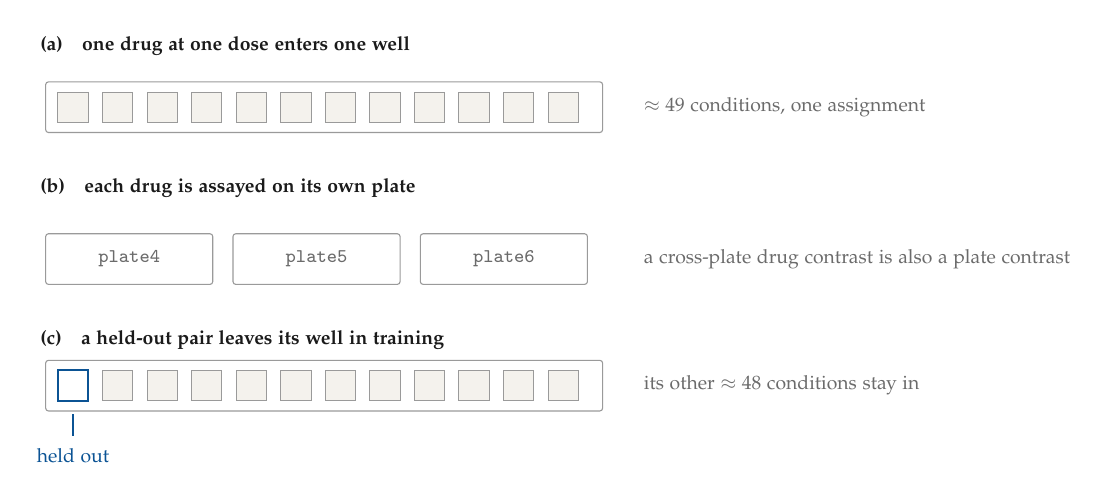
\begin{tikzpicture}[x=1.286cm, y=1.286cm, font=\small,
  lane/.style={draw=rulegrey, line width=0.4pt, rounded corners=1pt},
  cellb/.style={draw=rulegrey, line width=0.3pt, fill=panelbg,
                minimum size=3.86mm, inner sep=0pt},
  outb/.style={draw=accent, line width=0.7pt, fill=white,
               minimum size=3.86mm, inner sep=0pt},
  lbl/.style={font=\scriptsize, text=quietink},
  strong/.style={font=\scriptsize\bfseries, text=ink}]

% (a)
\node[strong, anchor=west] at (0,3.95)
  {(a)\quad one drug at one dose enters one well};
\draw[lane] (0.15,3.10) rectangle (5.65,3.60);
\foreach \i in {0,...,11}{\node[cellb] at (0.42+\i*0.44,3.35) {};}
\node[lbl, anchor=west] at (5.961,3.35)
  {$\approx 49$ conditions, one assignment};

% (b)
\node[strong, anchor=west] at (0,2.55)
  {(b)\quad each drug is assayed on its own plate};
\foreach \p/\x in {4/0.15, 5/2.00, 6/3.85}{
  \draw[lane] (\x,1.60) rectangle (\x+1.65,2.10);
  \node[lbl] at (\x+0.825,1.85) {\texttt{plate\p}};}
\node[lbl, anchor=west] at (5.961,1.85)
  {a cross-plate drug contrast is also a plate contrast};

% (c)
\node[strong, anchor=west] at (0,1.05)
  {(c)\quad a held-out pair leaves its well in training};
\draw[lane] (0.15,0.35) rectangle (5.65,0.85);
\node[outb] at (0.42,0.60) {};
\foreach \i in {1,...,11}{\node[cellb] at (0.42+\i*0.44,0.60) {};}
\draw[accent, line width=0.4pt] (0.42,0.32) -- (0.42,0.10);
\node[lbl, anchor=north, text=accent] at (0.42,0.08) {held out};
\node[lbl, anchor=west] at (5.961,0.60)
  {its other $\approx 48$ conditions stay in};

\end{tikzpicture}%

\caption[The well is the unit the atlas actually assigns]{\textbf{One
assignment, many conditions.} The roughly $49$ conditions from one well share
an assignment and a batch (a). Each drug is assayed on its own plate or plates,
so a drug contrast across plates is also a plate contrast (b). Removing a (drug,
cell line) pair leaves its well in training through the other $\approx 48$ lines
(c). Squares are conditions, twelve per well for legibility.}
\label{fig:confound}
\end{figure}

\begin{defn}{Condition, treated well, batch unit}
A \emph{condition} is a (drug, cell line, plate, dose) tuple, and it is the unit
everything below is scored at. The physical assignment is the \emph{treated
well}, so a condition sits inside an assignment and is not one. Plates are
numbered within cell line, not globally, so the batch unit is the pair (cell
line, plate), never the plate label alone. A \emph{pseudobulk} is a group's mean
expression profile; a \emph{control pseudobulk} is the same over plate-matched
DMSO cells.
\end{defn}

Dose is a molar concentration resolved from \texttt{drugname\_drugconc}; an
earlier pipeline kept only the numeric part, which collides $1\,\mu$M with
$1\,$nM. An audit of all $289$ treated wells found $289$ usable molar doses
with zero unit collisions, so the defect was a demonstrated possibility that did
not materialise. Combination treatments are dropped, not analysed as their first
component.

\begin{scopelimit}[carried into \cref{sec:methods-holdout} and \cref{sec:limitations}]
A (drug, cell line) pair cannot be held out cleanly on this cache. Removing the
pair removes one condition, and its well remains in training through the other
$\approx 48$ lines. The residual arm therefore builds its own, larger holdout.
\end{scopelimit}

\section{Barely half the atlas is identifiable}

\cref{tab:scale} states the quantities every $n$ in the investigation should be
located against. One symbol in it runs ahead of its
derivation.\seealso{\cref{sec:res-metrics} derives $\NIR$ and audits its chance
level with empirical control arms.} $\NIR$, the normalised inverse rank, is the
fraction of a declared comparison set whose truth a prediction resembles less
than its own, so chance is $0.50$ under the exchangeability condition of
\cref{sec:res-metrics}.

\begin{scopelimit}[carried into \cref{sec:res-blind} and \cref{sec:res-encoding}]
Two populations are used and they are not interchangeable. The broad
characterisation (\cref{sec:res-blind}) streams a wide sample of the atlas, over
more plates and drugs than cached, so the drug and condition counts in its block
of \cref{tab:scale} count that sample, not the cache. The residual arm
(\cref{sec:res-encoding} onward) works from a smaller cached subset. A count
from one block does not bound a count in the other.
\end{scopelimit}

\begin{table}[htbp]
\begin{fullwidth}
\begin{threeparttable}
\caption{\textbf{The populations behind every $n$ quoted in the investigation.}
The upper block is a streamed sample of the atlas; the lower two are the cache
built once and reused.}
\label{tab:scale}
\small
\centering
\begin{tabular}{p{0.64\linewidth}r}
\toprule
\multicolumn{2}{l}{\thead{Task characterisation} (streamed sample)} \\
\midrule
conditions characterised & \num{6628} \\
\hangindent1em\hangafter0 of which statistically active against DMSO & 3,647 / 5,014 (72.7\%) \\
\hangindent1em\hangafter0 empirically identifiable at the tested pseudobulk budget (own within-plate
  split-half $\NIR \geq 0.8$) & 3,064 (46.2\%) \\
\hangindent1em\hangafter0 with a plate-mate closer than their own split-half & 78.7\% \\
median cells per condition & 44 \\
median \#DEGs per condition (BH $q<0.05$) & 0 \\
median SNR (effect $\div$ within-well split-half noise) & 0.75 \\
drugs with a real dose series & 218 / 351 (62.1\%) \\
drugs seen in $\geq 3$ cell lines & 227 \\
\midrule
\multicolumn{2}{l}{\thead{Residual-frame cache} (rebuilt targets,
  \cref{sec:methods-residual})} \\
\midrule
cells (treated / control) & 620,564 (600,000 / 20,564) \\
(cell line, plate) groups behind scored conditions & 119 \\
drugs / cell lines & 106 / 50 \\
conditions with $\geq40$ treated and $\geq20$ control cells & 6,617 \\
\hangindent1em\hangafter0 by split after inventory filters (train / held-out wells / held-out drugs)
  & 4,999 / 900 / 711 \\
\hangindent1em\hangafter0 retained by the data-resolved reliability line & 2,523 of 4,999 train
  (50.5\%) \\
training examples / well-held-out validation examples & 147,710 / 3,600 \\
\midrule
\multicolumn{2}{l}{\thead{Evaluation sets}} \\
\midrule
tier 1 (seen conditions) / tier 2 (unseen drugs) / tier 3 (unseen combinations)
  & 4,325 / 2,188 / 99 \\
conditions scored per tier, generation evaluations & 400 \\
\raggedright tier-2 conditions in the expression-frame $\NIR$ benchmark
  (within plate) & 606 \\
conditions scored in the residual-frame evaluation & 1,394 \\
\hangindent1em\hangafter0 by split (train / \texttt{unseen\_combo} / \texttt{unseen\_drug})
  & 300 / \needsaudit{895} / 199 \\
\hangindent1em\hangafter0 treated wells behind them (no well spans two splits) & 136 / 36 / 28 \\
\hangindent1em\hangafter0 drugs per split (90 distinct in total) & 76 / 34 / 10 \\
\hangindent1em\hangafter0 cell lines per split (42 distinct in total) & 39 / 42 / 40 \\
\bottomrule
\end{tabular}
\begin{tablenotes}[flushleft]\footnotesize
\item The $72.7\%$ figure is over the $5{,}014$ conditions whose (cell line,
plate) group carries plate-matched DMSO cells, not all $6{,}628$.
\item The identifiability bar is per-condition, distinct from the aggregate
ceilings of \cref{tab:ceilings}.
\item The \texttt{unseen\_combo} count is flagged pending a cluster rerun; no
argument turns on its exact value.
\end{tablenotes}
\end{threeparttable}
\end{fullwidth}
\end{table}

\paragraph{The upper block is a result} It describes Tahoe-100M, not this
project. Across the $5{,}014$ control-reachable conditions the median has no
differentially expressed gene at BH $q<0.05$ and a signal-to-noise ratio of
$0.75$ against its own within-well split-half noise, while $72.7\%$ are active
on the whole profile, leaving $27.3\%$ statistically inert. A per-gene test is
far harsher, and $27.3\%$ alone would make the atlas sound better resolved than
it is. The typical condition carries a real response
measured with too few cells, and not no response (\cref{sec:res-blind}).

The identifiability bar is per-condition: a condition's own split-half $\NIR$
against its plate-mates has to clear $0.8$. Of the $6{,}628$ conditions,
$46.2\%$ clear it, and $78.7\%$ have a plate-mate lying closer to them than
their own second half does. Identifiability is a property of the pairing, not of
the drug: over the $227$ drugs assayed in at least three cell lines, the median
drug's split-half reference spans $0.83$ between its most and least identifiable
context (\texttt{drug\_biology\_atlas.json}). A benchmark omitting those figures
quotes accuracies over a population barely half of which is empirically
identifiable at the tested pseudobulk budget, and a per-drug leaderboard on it
ranks pairings.

% The term is first used in tab:scale above, inside a float, where a marginpar
% cannot be set. This is its first prose use and the chapter's definition point,
% per the \gloss convention (definition at first use in each chapter). Wording
% is the one 05-Limitations.tex already uses, so the two agree word for word.
\paragraph{A filter this table does not total} The middle block records
$2{,}523$ of $4{,}999$ training conditions as \emph{retained by the
data-resolved reliability line},\gloss{reliability line}{The half-split cosine
threshold above which a condition's residual counts as reproducible.} which
\cref{sec:methods-residual} resolves from the data and applies to the training
split alone. It does not state the pool
once the held-out splits join that filtered set. The channel gate of
\cref{sec:res-scope} later scores \needsaudit[the retained pool]{4{,}131}
retained conditions; a cluster rerun settles whether that is this table's
three-way tally under another name, and no figure here depends on it.

The three tiers of the last block are defined by what training contained.
\emph{Tier 1} holds conditions whose (drug, cell line) pairing was
seen in training, so it measures fit and not generalisation. \emph{Tier 2} holds
conditions whose drug never appeared, Leave-Drugs-Out in the vocabulary of
\cref{sec:lit-dreval}. \emph{Tier 3} holds pairings whose drug and cell line
were each seen but never together, Leave-Pairs-Out; it is small ($99$
conditions) and is reported only where adequately powered. The residual arm
builds its own, larger holdout instead: \cref{sec:apparatus-vocab} names its
three splits, and \cref{sec:methods-holdout} settles the unit they are keyed
at.

\section{The backbone has seen no perturbation}

A cell is written as a \emph{cell sentence}, its expressed panel genes in
descending order, terminated by \ENDCELL. The prompt supplies cell line, drug,
dose, mechanism and the control cell's sentence; what the model must produce is
the treated cell's. \ENDCELL{} and (for the residual arm) \DOWN{} are registered
as atomic special tokens; unregistered, \DOWN{} splits into sub-words and the
up/down boundary stops being a clean symbol.

The backbone is \texttt{C2S-Scale-Pythia-1b-pt}~\cite{c2sscale}, a C2S-Scale
checkpoint on the Pythia-1b decoder~\cite{pythia}, cold-started for every arm
from the same base checkpoint with identical hyperparameters (1 epoch, learning
rate $10^{-5}$, gradient accumulation 16, maximum length 8192,
bf16).\seealso{\cref{sec:appendix} tabulates the training arms.} Cold-starting
makes the arms comparable; the training target or objective is the only
variable.

\paragraph{What the checkpoint has seen} It is pretrained on over 50 million
human and mouse cells from 825 single-cell datasets in CELLxGENE and the Human
Cell Atlas, an atlas corpus with no chemical or genetic perturbation data. Its
model card lists cell and tissue prediction, conditioned generation and gene-set
conversion, but not perturbation prediction. The base model arrives at
fine-tuning here having never seen a drug-treated cell.

\paragraph{Two channels stay open} The decoder underneath is Pythia-1b,
pretrained on text in which drug names, targets and mechanisms occur, and every
prompt supplies the drug's \texttt{moa-fine} annotation. A drug the fine-tuning
never saw is not a drug the system knows nothing about.

\begin{scopelimit}[carried into \cref{sec:res-scope} and \cref{sec:limitations}]
``Held out'' therefore means held out from Tahoe fine-tuning, with mechanism
supplied, and every unseen-drug result below is read under that narrower scope.
\end{scopelimit}

\section{The generic replaces the target}
\label{sec:apparatus-vocab}

Two \emph{measurement frames} run through the investigation and are never
interchangeable (\cref{fig:frames}): the \emph{expression frame} scores a
predicted cell profile against other drugs on the same plate, the
\emph{residual frame} (\cref{sec:methods-residual}) scores the drug-specific
residual against other drugs in the same cell line. Both put chance at $0.50$. The
\emph{comparison set} $J$, the conditions a prediction is ranked against, is
what fixes it there, and it is declared at every score below. A score without
its comparison set is not a score.

% ===========================================================================
% frames.tex -- the two measurement frames, EXPR and RESID, as two cards.
% \input by Sections/03-Apparatus.tex. Compiles against thesis_v2/preamble.tex
% and nothing else; no external data, no \includegraphics.
%
% NO DATA SOURCE. This is a schematic. The only numeral on the cards is the
% chance level 0.50, which is a definition and not a measurement: both frames
% are two-alternative retrievals, so chance is 0.50 by construction. It agrees
% with the prose immediately above this figure in Sections/03-Apparatus.tex
% ("Both put chance at $0.50$"), with Sections/02-Background.tex:244 and with
% Sections/04a-ruler.tex:530 ("Chance is $0.50$ by ..."). Nothing here is read
% from RESULTS_cluster/ because nothing here is a result. The numeric version
% of this argument -- the two frames on their own scales -- is fig:two-scales
% in 04d; Chapter 3 is apparatus and comes before those results exist, so this
% figure carries no scale, no axis and no measured quantity. Sibling
% frames.json records the geometry and that single number.
%
% ---------------------------------------------------------------------------
% THE BUG, AND WHY THE FIX IS NOT THE ONE-LINER IT LOOKS LIKE.
%
% Symptom, both cards: the two-line value on row 2 collided with its own key.
% Measured in the built thesis, ink gap between the key and its value, in
% PostScript points: r1 -0.02, r2 -3.02, r3 +2.12. Only r2 is visible as a
% collision. (r1 is the descender of "predicted" level with the ascender of
% "profile"; different x, they do not touch.)
%
% Diagnosis, as briefed and confirmed: val/.style used anchor=WEST, which
% centres a node's box on its y, so a TWO-LINE value grew upward into the key
% above it while one-line values did not.
%
% The briefed fix was anchor=north west with every value at its key's
% y - 0.30cm. Built, that removes the collision and introduces a worse fault:
% it lowers each value until it sits CLOSER TO THE NEXT KEY THAN TO ITS OWN,
% so every value reads as the heading of the row beneath it. Sweeping the
% offset, all measured inside one PDF by tools/_measure_frames.py and recorded
% in frames.json, gave "within" = key to its own value, "between" = value to
% the next key:
%
%   offset      within r1 / r2 / r3      between: after r1 / after r2
%   0.15          2.21  2.24  3.14            9.60        7.43
%   0.30          6.46  6.49  7.39            5.35        3.18   <- reversed
%   0.40          9.29  9.33 10.23            2.51        0.35
%
% and then the same figure BUILT INSIDE THE THESIS at offset 0.15 measured
% 5.95 / 5.98 / 5.29 within against 5.86 / 3.69 between -- 3.7pt away from the
% harness, and ambiguous. The offset is not a constant of the figure.
%
% ROOT CAUSE, and why this file no longer uses align=left. TikZ's `align'
% option typesets the node in a minipage, and a minipage's first-line height
% follows the AMBIENT \baselineskip. So a value node's ink lands in a place
% that depends on the prose that happens to precede the float: about 2.2pt
% between a \normalsize paragraph and a \small line, and about 3.7pt between a
% test harness and Chapter 3. No choice of offset survives an edit to the
% surrounding text. Calibrating one would have hidden the fault, not fixed it.
%
% THE FIX ACTUALLY USED: every node is a single line anchored BASE WEST, so
% each y coordinate below IS that line's baseline. Nothing is centred, nothing
% is measured from a box edge, no minipage is created, and no ascender or
% descender can move a line. The two-line value is two nodes rather than one
% node with `\\'. Key-to-value leading is therefore identical on all three rows
% and on both cards by construction -- which is what the brief asked for -- and
% it is now also identical from build to build.
%
%   key baselines    3.70   2.72   1.52     (row pitch unchanged)
%   value baselines  3.37   2.39   1.19     (key - 0.33cm)
%   row-2 value, second line  2.06          (previous line - 0.33cm)
%
% ONE step governs everything inside a row: 0.33cm = 9.39pt, one \scriptsize
% line of leading. A key and its value therefore set as two consecutive lines
% of a single block, exactly as rows 1 and 3 of the published figure did, and a
% wrapped value continues on the same rhythm. Row SEPARATION is carried
% entirely by the key pitch, which is untouched (0.98cm, then 1.20cm), giving
% 0.65cm and 0.53cm of clear space before the next key -- roughly twice the
% within-row step, so a value binds to the key above it and not to the one
% below.
%
% Verified by reading the baselines back out of the built PDFs. Chapter 3 in
% main.pdf and all four contexts of figs/_frames_harness.tex report the same
% seven baselines to 0.001cm:
%   3.703  3.375 | 2.727  2.398  2.059 | 1.531  1.203   (tikz y, both cards)
% Note the harness and the thesis are only comparable on BASELINES. Glyph
% bounding boxes reported by a PDF text extractor differ by a constant ~2.1pt
% between the two files because the font subsets differ, so ink-gap numbers
% are only meaningful WITHIN one PDF.
%
% OTHER LAYOUT NOTES
%   * cards are 5.9cm wide with a 0.5cm gutter, 12.3cm overall. NOT rescaled:
%     12.3cm sits inside the 14.2cm body block and leaves the page free to
%     carry a margin note.
%   * the dotted rule and the sentence under it span BOTH cards on purpose.
%     They are the only mark that crosses the gutter; everything else is
%     card-local, because the point of the figure is that the columns do not
%     exchange.
%   * if a value ever needs a third line, add a node at (its predecessor
%     - 0.34cm). Do not reintroduce align/`\\'.
% ===========================================================================
\begin{figure}[htbp]
\centering
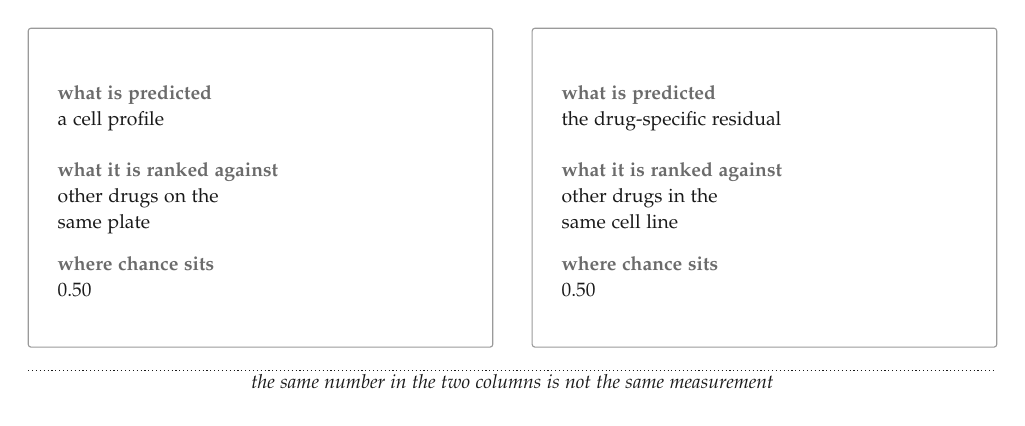
\begin{tikzpicture}[x=1cm, y=1cm, font=\small,
  panel/.style={draw=rulegrey, line width=0.4pt, rounded corners=1pt},
  % base west on both: every y below is a BASELINE. See the header note --
  % anchor=west centres the box (that was the collision) and align=left makes
  % the node's height depend on the surrounding prose (that was worse).
  key/.style={font=\scriptsize\bfseries, text=quietink, anchor=base west},
  val/.style={font=\scriptsize, text=ink, anchor=base west}]

\draw[panel] (0,0.55) rectangle (5.9,4.6);
\draw[panel] (6.4,0.55) rectangle (12.3,4.6);

\node[anchor=base west] at (0.25,4.18) {\Eframe};
\node[anchor=base west] at (6.65,4.18) {\Rframe};

% key baseline 3.70 / 2.72 / 1.52 ; value baseline = key - 0.33 ; wrap - 0.34.
\node[key] at (0.25,3.70) {what is predicted};
\node[val] at (0.25,3.37) {a cell profile};
\node[key] at (6.65,3.70) {what is predicted};
\node[val] at (6.65,3.37) {the drug-specific residual};

\node[key] at (0.25,2.72) {what it is ranked against};
\node[val] at (0.25,2.39) {other drugs on the};
\node[val] at (0.25,2.06) {same plate};
\node[key] at (6.65,2.72) {what it is ranked against};
\node[val] at (6.65,2.39) {other drugs in the};
\node[val] at (6.65,2.06) {same cell line};

\node[key] at (0.25,1.52) {where chance sits};
\node[val] at (0.25,1.19) {$0.50$};
\node[key] at (6.65,1.52) {where chance sits};
\node[val] at (6.65,1.19) {$0.50$};

\draw[ink, line width=0.4pt, densely dotted] (0,0.25) -- (12.3,0.25);
\node[font=\scriptsize\itshape, text=ink, anchor=base] at (6.15,0.02)
  {the same number in the two columns is not the same measurement};
\end{tikzpicture}
\caption[The two measurement frames]{\textbf{Two frames, one chance level, and
no exchange rate between them.} The prediction, the comparison set and the
meaning of a score change between frames; the chance level does not.}
\label{fig:frames}
\end{figure}


\begin{defn}{The generic and the residual target}
The \emph{generic} is the drug-agnostic mean response subtracted to form the
residual, operationally the mean shift over the other drugs at the stated scope,
conventionally read as the stress and cell-cycle programme common to all
drugs --- a reading used for intuition and nowhere tested. The
\emph{residual target} is what remains. It is built \emph{split-before-fit}
(holdout fixed from metadata before any statistic is estimated) and
\emph{leave-one-drug-out} (no condition's generic contains its own drug). The \emph{scope}, \texttt{cell\_line} or \texttt{plate}, is the set
of drugs the mean is taken over.
\end{defn}

The generic carries $39.0\%$ of the perturbation shift's energy
(\cref{sec:res-transfer}), so subtracting it does not clean the target up but
replaces it: every residual-frame number is a score on what is left.

\paragraph{Baselines and splits} \emph{Control-copy} predicts the untreated cell
unchanged; carrying zero drug information, it is the floor a drug-aware model
has to clear. The residual arm's split has three parts,
\texttt{train}, \texttt{unseen\_combo} (an unseen \emph{well} of a seen drug)
and \texttt{unseen\_drug}, sampled under an explicit per-split \emph{quota},
because a uniform draw reproduces the pool's proportions and starves the
held-out splits (\cref{sec:methods-holdout}). Five training \emph{arms} differ
only in target or objective; where a claim is multiplicity corrected, the family
is those five by up to seven depths.

\section{One estimator, and not a replicate}

Almost every negative result below is stated as a distance from a
\emph{ceiling}. The word names one estimator, not seven.

\begin{defn}{Within-well split-half precision reference}
The score obtained when a disjoint cell subset of the same treated well is
substituted for the prediction, recomputed for every stratum scored, so its
value moves with the stratum. It is not a replicate ceiling. What varies across
the rows of \cref{tab:ceilings} is the frame, the comparison set and the cell
budget, never the estimator.
\end{defn}

Two properties limit how the ceilings read. First, they are \emph{split-half}
estimates and not biological replicates, because this cache places $286$ of
$287$ treatments in exactly one well. Second, a split-half ceiling estimates
within-well sampling precision, which is optimistic relative to true biological
reproducibility, and every coverage figure in \cref{sec:res-lookup} inherits
that optimism.

\paragraph{The one exception} One ceiling is not that estimator and not a row in
\cref{tab:ceilings}. The positive control inside the expression-frame $\DRF$
audit of \cref{sec:res-metrics} is a denoised interpolated duplicate, not a raw
split-half, and that section turns on the difference.

\begin{table}[htbp]
\begin{fullwidth}
\begin{threeparttable}
\caption{\textbf{One estimator, seven settings.} Every ``ceiling'' here is a
within-well split-half precision reference, the score of a disjoint subset of
the same treated well's cells. They differ in frame, comparison set, cell budget
and split contents.}
\label{tab:ceilings}
\footnotesize
\begin{tabularx}{\linewidth}{@{}>{\raggedright\arraybackslash}p{0.18\linewidth}
  >{\raggedright\arraybackslash}p{0.20\linewidth}
  >{\raggedright\arraybackslash}p{0.31\linewidth}X@{}}
\toprule
\thead{Ceiling} & \thead{Frame and metric} & \thead{Comparison set and budget}
  & \thead{Where used} \\
\midrule
$0.76$ & expression, $\DEdr$ & two real cells & metric audit
  (\cref{sec:res-metrics}) \\
$0.625$ / $0.575$ & expression, $\NIR$ & leak audit; cross-plate / within plate
  & plate leak (\cref{sec:res-blind}) \\
$0.67$--$0.83$ & expression, forced choice & within plate, by cell budget
  & \cref{sec:res-blind} \\
$0.576$ & expression, $\NIR$ & within plate, tier 2 & the blindness verdict \\
$0.61$ / $0.76$ / $0.85$ & expression, $\NIR$ & within plate;
  $10$/$40$/$120$ cells & identifiability curve \\
$0.956$/$0.824$/$0.836$ & residual, $\NIR$ & within cell line;
  train/combo/drug & \cref{sec:res-lookup} \\
$0.742$ / $0.7432$ & token retrieval & within condition, split-half
  & \cref{sec:methods-residual} \\
\bottomrule
\end{tabularx}
\begin{tablenotes}[flushleft]\footnotesize
\item The $\DRF$ positive control of \cref{sec:res-metrics} is the
investigation's one exception and is not a row here.
\item None of these is a biological replicate ($286$ of $287$ treatments sit in
a single well).
\item In the residual frame the raw reference is not constant across splits (a
spread of $0.132$), but that spread is an artefact of how the splits were
filtered and not a difference in recoverable signal; matched at the training
reliability line the three agree to $0.006$ (\cref{sec:limitations}).
\end{tablenotes}
\end{threeparttable}
\end{fullwidth}
\end{table}

\begin{scopelimit}[carried into \cref{sec:res-lookup} and \cref{sec:limitations}]
A distance to the reference is comparable within a split and not between them,
because the splits are scored on populations selected by different rules. And
because the reference is a sampling-precision estimate and not a biological
replicate, every coverage figure computed against it is a distance to an
optimistic bar by an unknown amount. Where one is quoted, the ordering carries
the claim.
\end{scopelimit}

\section{Two crossed dependencies, not one}
\label{sec:apparatus-clusters}

Two rules apply to every result below, plus one statement of provisionality.
Conditions are not independent, and not independent in two crossed ways at once
(\cref{fig:clustering}): two from one treated well share a physical assignment
and a batch, two from one cell line share the biology. Treating them as
independent gives intervals about $1.5$ times too narrow on the scramble
strata and $1.7$ to $2.5$ times too narrow on the contrasts against the lookup
baselines. Clustering on the assignment unit alone uses the larger cluster
count ($289$ wells against $\approx 50$ lines) and would tighten every interval
while sounding more rigorous. That is the failure the estimator below avoids.

% ===========================================================================
% clustering.tex -- the two crossed groupings, plus the drug the wells nest in.
% \input by Sections/03-Apparatus.tex. Compiles against thesis_v2/preamble.tex
% and nothing else; SCHEMATIC -- no external data, no \includegraphics, and
% deliberately NO number anywhere in the drawing. The lattice is 9 columns of
% 6 dots because that is what reads at this measure, not because the cache
% holds 9 wells or 6 lines; the caption says so in as many words.
%
% WHY IT WAS REDRAWN. The version it replaces sat inline in 03-Apparatus.tex
% at lines 477-510 (v1's is under ../thesis/ and is not touched).
%
%   1. THE DOT WAS NOT ON THE LATTICE. The old bands were centred at y=2.6 and
%      x=5.0, while the lattice rows sat at 0.5+0.6r (2.3, 2.9) and the columns
%      at 0.7+1.1c (4.0, 5.1). Both centre lines fell BETWEEN dots, so the
%      accent "one condition" dot was drawn in the gap. The caption said "the
%      dot where they meet is one condition" and the drawing did not show one.
%      Here every coordinate is derived from the two constants the lattice is
%      generated from (\px, \py) and the highlight is addressed by INDEX
%      (\hc, \hr), so band centres and accent dot cannot drift off a lattice
%      point again.
%
%   2. THE BANDS WERE PADDED BY EYE. Old horizontal band 0.35..8.45 against
%      dots at 0.7..7.3 -- 0.35 short at the left, 1.15 long at the right. Old
%      vertical band 0.12..4.08 against dots at 0.5..4.1 -- 0.38 short at the
%      bottom, 0.02 over at the top. Here each band ends exactly half a lattice
%      pitch past its first and last dot (\BL,\BR,\BB,\BT below), computed, so
%      both are symmetric by construction.
%
%   3. THE DOTS WERE TEXTURE, NOT CONDITIONS. They were rulegrey!70, i.e.
%      #9A9A9A at 70% over white ~= #C0C0C0 -- lighter than the document's
%      quiet ink and far too light for a mark the caption asks the reader to
%      count. They are quietink (#6B6B6B) here, and 1.7pt rather than 1.5pt.
%
%   4. IT PAID FOR FULLWIDTH AND DID NOT USE IT. The old float opened
%      \begin{fullwidth} -- 174mm, and by the preamble's own rule a page
%      carrying one may then carry no margin note -- and drew 148.6mm. This
%      draws inside the 142mm measure (see MEASURED below), so it is an
%      ordinary body-width float and its page keeps the margin column.
%
%   5. THE DRUG WAS IN NO FIGURE AT ALL, and it is the axis that flips three
%      verdicts later. It is drawn in a deliberately different register from
%      the two bands: outline only, no fill, rounded corners, against two solid
%      tint rectangles. A well carries one drug at one dose (sec. "Every
%      treatment sits in one well"), so wells NEST inside drugs -- three whole
%      well-columns per envelope -- while the cell-line band CROSSES all three
%      envelopes and runs past the outer edge of both end ones. Nesting and
%      crossing are then the same picture, told apart by shape, not by colour.
%
% GEOMETRY, in cm, all of it derived from \px and \py. Every clearance here is
% computed from those two constants, not judged by eye:
%   lattice     9 cols x 6 rows, pitch 1.25 x 0.81, dots (0,0)..(10.00,4.05)
%   highlight   col 4 -> x = 5.00, row 4 -> y = 3.24     <- both ON the lattice
%   bands       half-thickness 0.25, so 0.155 of ground to the next dot row
%               (0.405 half-pitch - 0.25) and 0.095 clear of that dot's edge;
%               ends at -0.625/10.625 and -0.405/4.455, i.e. exactly half a
%               pitch past the first and last dot of the row and the column
%   envelopes   3 x 3 columns, pad 0.46 -> -0.46..2.96, 3.29..6.71, 7.04..10.46,
%               so 0.33 between neighbours; vertically -0.585..4.635, giving
%               0.18 of margin above and below the well band each one contains
%   callout     the leader leaves the accent dot at 46.3 deg, clears the
%               nearest lattice dot (6.25,4.05) by 0.354, and crosses the
%               middle envelope's TOP edge at x = 6.32, inside that envelope's
%               span 3.29..6.71 -- so it pierces one boundary and not two
%
% MEASURED, not estimated. figs/_harness_clustering.tex \input s this file
% against the real preamble, captures the float into a box with \caption and
% \label gobbled, and \typeout s \wd. Reading:
%   tikzpicture  385.40pt = 135.45mm wide, 187.44pt = 65.87mm tall
%   \textwidth   404.03pt = 142.00mm
%   fills 95.4% of the measure, 18.63pt = 6.55mm of slack.
% The build's overfull-hbox gate is 0; this figure contributes none. The
% fullwidth version it replaces drew 148.6mm against a 174mm allowance -- it
% overran the body measure, which is why it was in a fullwidth in the first
% place, and cost that page its margin column to do it.
%
% TYPE. \scriptsize on every label, matching fig:confound three pages earlier
% and fig:residual-energy in chapter 4. Deliberately not raised: this figure is
% read alongside fig:confound, and a lone larger label set would read as a
% different apparatus rather than as a corrected one.
% ===========================================================================
\begin{figure}[htbp]
\centering
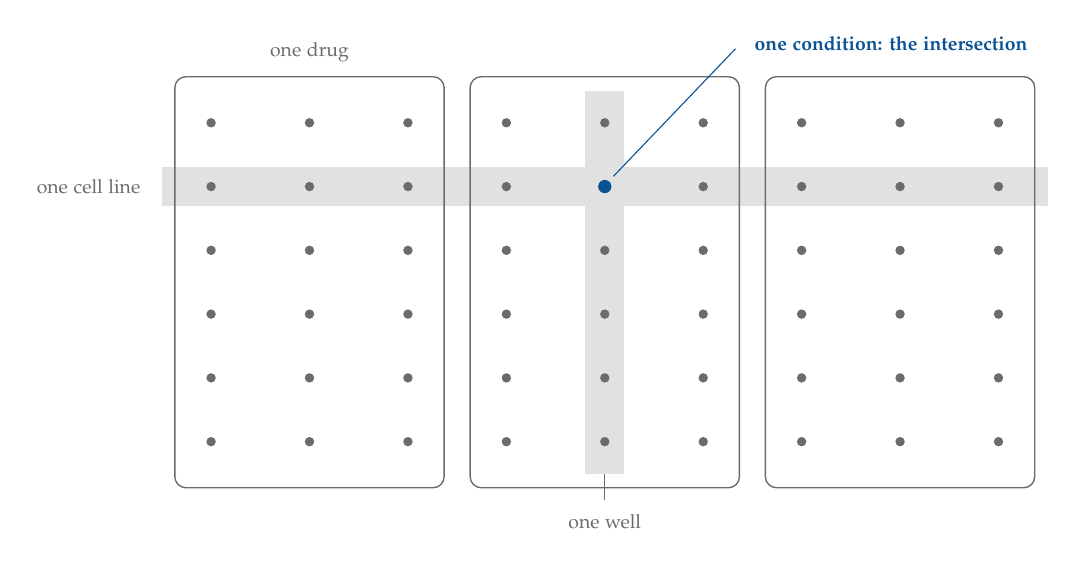
\begin{tikzpicture}[x=1cm, y=1cm, font=\small]
  % --- the constants everything else is derived from -----------------------
  \def\px{1.25}   % column pitch  (one well per column)
  \def\py{0.81}   % row pitch     (one cell line per row)
  \def\hc{4}      % highlighted column index, 0..8
  \def\hr{4}      % highlighted row index,    0..5
  \def\bt{0.25}   % half band thickness
  \def\ep{0.46}   % envelope padding around its three columns
  \def\vm{0.18}   % envelope margin above and below the well band

  \tikzset{
    cond/.style={fill=quietink},
    band/.style={fill=rulegrey!30},
    drugenv/.style={draw=quietink, line width=0.5pt, rounded corners=4pt},
    lead/.style={draw=quietink, line width=0.4pt},
    lbl/.style={font=\scriptsize, text=quietink},
    strong/.style={font=\scriptsize\bfseries, text=accent}}

  % centre lines of the two bands: ON the lattice, by construction
  \pgfmathsetmacro{\HX}{\hc*\px}            %  5.000
  \pgfmathsetmacro{\HY}{\hr*\py}            %  3.240
  % band ends: half a pitch past the first and last dot, both sides, both bands
  \pgfmathsetmacro{\BL}{-\px/2}             % -0.625
  \pgfmathsetmacro{\BR}{8*\px+\px/2}        % 10.625
  \pgfmathsetmacro{\BB}{-\py/2}             % -0.405
  \pgfmathsetmacro{\BT}{5*\py+\py/2}        %  4.455
  \pgfmathsetmacro{\EB}{\BB-\vm}            % -0.585
  \pgfmathsetmacro{\ET}{\BT+\vm}            %  4.635

  % ---- 1. the two crossed groupings, as solid tint bands ------------------
  \fill[band] (\BL,\HY-\bt) rectangle (\BR,\HY+\bt);      % one cell line
  \fill[band] (\HX-\bt,\BB) rectangle (\HX+\bt,\BT);      % one well

  % ---- 2. the drug, as an outline envelope over three whole well-columns --
  % It encloses the well band top and bottom as well as left and right, so the
  % well reads as INSIDE the drug and not merely beside it.
  \foreach \g in {0,1,2}{
    \pgfmathsetmacro{\GL}{3*\g*\px-\ep}
    \pgfmathsetmacro{\GR}{(3*\g+2)*\px+\ep}
    \draw[drugenv] (\GL,\EB) rectangle (\GR,\ET);}

  % ---- 3. the conditions --------------------------------------------------
  \foreach \c in {0,...,8}{
    \foreach \r in {0,...,5}{
      \fill[cond] (\c*\px,\r*\py) circle (1.7pt);}}

  % ---- 4. the intersection ------------------------------------------------
  \fill[accent] (\HX,\HY) circle (2.4pt);
  \draw[accent, line width=0.4pt]
    (\HX+0.11,\HY+0.13) -- (\HX+1.66,\HY+1.75);
  \node[strong, anchor=west] at (\HX+1.78,\HY+1.81)
    {one condition: the intersection};

  % ---- 5. direct labels, one per grouping. No legend, no key. -------------
  % cell line: to the left of its own band.
  \node[lbl, anchor=east] at (\BL-0.15,\HY) {one cell line};

  % well: below its own band, on a lead that PIERCES the envelope's lower
  % edge -- the crossing of that boundary is the nesting, drawn.
  \draw[lead] (\HX,\BB) -- (\HX,\BB-0.34);
  \node[lbl, anchor=north] at (\HX,\BB-0.40) {one well};

  % drug: above the leftmost envelope, centred on it. Placed there and not on
  % the middle envelope because the middle one is where the well band and the
  % callout leader already are, and "one drug" centred over the highlighted
  % column would compete with "one well" for the same column.
  \node[lbl, anchor=south] at (\px,\ET+0.06) {one drug};

  % NO free-floating note line. The version this replaces carried "neither
  % grouping is nested in the other" as a caption-width sentence under the
  % lattice. Two reasons it is gone: the caption now states it in the same
  % words, and at page scale a \scriptsize sentence sitting 4mm above
  % "Figure 3.3." reads as the caption's first line rather than as part of the
  % drawing. The claim is not dropped -- it moved into the caption, where the
  % new drug clause needs it anyway.
\end{tikzpicture}
\caption[The two crossed groupings, and the drug the wells nest in]{\textbf{A
condition belongs to a well and to a cell line at once, and the two groupings
cross.} Each dot is a condition; the horizontal band is one cell line, the
vertical band one well. The dot where they meet is one condition, which is why
the intersection term is the ordinary independent-sampling variance. The
rounded envelopes are drugs: a well carries one drug at one dose, so wells nest
inside drugs, while the cell-line band crosses every drug and neither of the
two bands is nested in the other. The lattice is schematic --- nine columns of
six, for legibility, and not a count of anything in the cache.}
\label{fig:clustering}
\end{figure}


Every interval on a \emph{mean} is therefore two-way cluster-robust
(Cameron--Gelbach--Miller),
\begin{equation}
 V \;=\; V_{\textrm{line}} \;+\; V_{\textrm{well}} \;-\; V_{\textrm{intersection}},
\end{equation}
where the intersection of the two groupings is the single condition, so
$V_{\textrm{intersection}}$ is the ordinary independent-sampling variance. When
it goes non-positive in a finite sample, the wider one-way variance is used and
the branch recorded. The formula above is valid only where the two groupings
genuinely cross, which cell line and well do: a treated well spans
$\approx 49$ cell lines and a cell line recurs across wells. Drug and well do
\emph{not} cross, because one drug is assigned per well and wells therefore nest
strictly inside drugs. Where an interval is reported on the drug axis the
estimator tests the two groupings for nesting first and, finding it, clusters
one-way on the drug rather than applying the expression above to a nested pair;
the branch taken is recorded beside the interval. Reading ``two-way'' as
``the equation above was applied to drug and well'' would therefore be wrong.
It is asymptotic in clusters, so the reference distribution
is Student's $t$ with one fewer degree of freedom than the smaller cluster
count. The \texttt{unseen\_drug} arm shows what that costs: \cref{tab:scale}
puts $199$ scored conditions behind it, drawn from $28$ treated wells and $40$
cell lines, so the smaller cluster count is the $28$ wells, the reference is
$t_{27}$ and not the normal, and the interval widens by $4.7\%$.

For statistics over pairs of conditions, such as the transfer coefficient,
neither grouping partitions the pairs, so those intervals use the
Fafchamps--Gubert dyadic estimator, under which two pairs are dependent when
they share either member.

Throughout, an estimate is quoted as value [lower, upper], a two-way
cluster-robust $95\%$ interval unless stated otherwise. DrEval~\cite{dreval}
identifies the same structure more broadly, citing Hurlbert~\cite{hurlbert}:
hundreds of thousands of cells resolving to a few hundred conditions over $50$
cell lines.

\section{The generation budget is part of the claim}

The second rule concerns generation validity. The budget is a claim-level
variable, not a runtime setting.

A $600$-token cap truncated $26\%$ of predictions in an early run, silently,
because nothing measured them. A prediction cut at the cap never reaches \DOWN{}
and is scored with its whole down-block missing, and no completion rate was
quoted beside the score.

\paragraph{What it cost} The optimal-transport arm of
\cref{sec:res-epsilon}, scored at that cap, gave a gap of
\ci{+0.0144}{-0.0051}{+0.0338} against its geometry-defined \texttt{orth}
partner, whose observed score is near chance. That interval spanned zero and the
arm was printed as inert.\corrmark{The printed negative is retracted in
\cref{sec:res-encoding}, in full and where it was made.} Re-run at the $1400$
tokens the residual arm had, it gives \ci{+0.0292}{+0.0144}{+0.0441}, and the
negative had to be withdrawn (\cref{sec:res-encoding}). The same cap had already
halved the residual arm's own effect. Wherever a paired comparison is scored on
variable-length predictions, then, the token budget is part of the claim, and a
null quoted without its budget cannot be read.

\paragraph{The rule that follows} Every generation-based evaluation computes the
\ENDCELL{}/\DOWN{} completion rate, the fraction of emitted symbols that are
valid panel genes, and the duplicate rate before any score is read from it, and
no score below comes from a run whose validity block was not inspected.

The intervals do not cover the generation configuration. Sampling is at
temperature $0.8$ with top-$p$ $0.9$ throughout, over four budgets: $1200$
tokens with eight predictions per condition in the expression-frame evaluations
feeding \cref{sec:res-blind} and \cref{tab:epsilon}; $1400$ with four in the
residual-frame evaluations of \cref{sec:res-encoding}; $600$ with four in the
control arms until re-run at the residual arm's budget; and $3800$ for output
invariance, which compares whole predictions and is not truncated to a scoring
panel. Where a null turns on its budget the budget is named there, and every
contrast uses a fixed per-(condition, arm) seed.

% PLACEMENT: at the previous setting this box split across the chapter's last
% page break, carrying two lines onto a page that is otherwise almost empty.
% The box is ~9 lines; ask for enough room to keep it whole.
\needspace{10\baselineskip}
\begin{scopelimit}[carried into every residual-frame number below]
Every residual-frame number comes from one generation run and its companion
audits (\texttt{re\_v3} with the scramble-stratum audit, the matched variance
decomposition, the two calibration runs and the channel gate). Numbers from the
two earlier runs are not reconciled with these and are not quoted, except where
a superseded estimate is named as such and the conclusion drawn from it
withdrawn, because between runs the sign of several estimates changed and not
only their magnitude.
\end{scopelimit}

Two components carried defects found after that run and have since been repaired
and re-run, the $\DRF$ calibration bootstrap (\cref{sec:res-metrics}, both arms)
and the channel-gate partner pool (\cref{sec:res-scope}); both are reported on
the corrected runs.

That is the apparatus. It settles what is measured, on what population, against
what reference and with what uncertainty, and reaches no verdict about the
model.

% Chapter 4 is ONE chapter in four physical files. It uses \include for the
% chapter and \input for the four parts (inside 04-Investigation.tex), because
% \include forces a \clearpage and four of those would fall at arbitrary points
% inside a single continuous argument.
% 04-Investigation.tex -- chapter wrapper. The four parts are \input, not
% \include, so no \clearpage is forced inside one continuous argument.
%
% The opener carries three things and nothing else: the six findings as a
% numberless skeleton, the chronological principle, and fig:timeline as the
% full nine-beat map. Sources in v1: thesis/Sections/Investigation-v4.tex
% 27-49 (the chronological principle), 51-84 (the six findings) and 86-112
% (the timeline figure and its caption).
%
% NO NUMBERS ANYWHERE IN THIS FILE. That is a rule, not an accident. v1's
% organiser put the findings and their quantities in one ~1,100-word block
% that tried to be both a map and a complete record and became neither. Every
% figure quoted below in v1 (the coverage percentages, the annotated-drug
% count, the layer depths) is established, qualified and scoped in the beat
% that owns it, and is quotable only from there.
%
% fig:timeline is redrawn, not copied from v1. The v1 layout ran 4+4+1 and
% routed the row connectors straight through the nodes of the row below.
% This one snakes 3+3+3, so no connector crosses a node. Same nine beats, same
% order, same caption claim.
%
% The b2 node is the one to watch. Beat 2 (sec:res-blind) landed in
% 04a-ruler.tex only after this opener was drafted, and until it did, "nine
% beats" was a promise the chapter could not keep and the front matter's
% \seealso at 00-HowToRead.tex:46 pointed at a figure that did not exist. Both
% now resolve. If beat 2 is ever moved or renamed, this figure and that
% \seealso are the two places that break.
\chapter{The investigation, in the order it happened}
\label{sec:methods}
\label{sec:results}
\framedecl{ER}

\begin{question}
Does a model that has learned something about a drug answer differently when it
is told a different drug? The question is cheap to ask and expensive to ask
honestly, because the instrument had to be measured before the model could be.
Each beat below builds the tool that the measurement before it made necessary.
\end{question}

\noindent
The order is chronological, not the order that would argue best. That is
load-bearing: a design choice appears as the failure it avoids, and a dead end
appears where it was walked into. The apparatus is \cref{sec:methods-data}; the
terms, symbols and conventions are fixed in \nameref{sec:howtoread}.

\paragraph{The findings, before the beats that produced them} Six, in the order
they arrived, with no numbers attached. Each one is established, qualified and
scoped in the beat that owns it, and is quotable only from there. What follows
is a skeleton, not a record.

\begin{itemize}
\item The ruler was wrong. The field's standard perturbation metric is saturated
  by a predictor that carries no drug information at all, so the instrument was
  repaired before the model was measured.
\item On the repaired instrument the model is drug-blind in the expression
  frame. It returns the same answer whether told the true drug or a different
  one, and a baseline that copies the untreated cell matches it.
\item The blindness is not a failure to encode. Drug identity is written into
  the activations at every layer measured, and generation barely consults it.
  This is the chapter's least well-evidenced measurement.
\item Re-encoding the training target as the drug-specific residual makes the
  model demonstrably sensitive to the drug in its prompt. That is the project's
  first non-null drug effect: first in sequence, and not the only target
  construction that produces one.
\item Responding to the drug is not predicting it. Prompt sensitivity survives a
  holdout of whole treated wells; biological transfer to those wells is
  \notestablished on the axis a drug-specific claim has to generalise across, and
  a lookup table of training averages outscores the model. That dissociation is
  this chapter's argument.
\item For a drug the model has never seen, same-target retrieval is the
  strongest observed lead on its own restricted support; mechanism and chemical
  structure are inconclusive, not dead.
\end{itemize}

\noindent
\Cref{fig:timeline} is the map. Nine beats produce those six findings; the ninth
produces none, and that is a decision, not work left undone.

% ---------------------------------------------------------------------------
\begin{figure}[htbp]
\centering
% The tikzpicture moved out to figs/timeline.tex in this revision. It was
% reworked, not relocated: box metrics only, contents untouched. The header
% comment of that file records the three faults it fixes (unaligned row tops,
% the hyphenated "A lookup ta-/ble wins", and the b3->b4 connector) and the
% width arithmetic behind the new column pitch. The float, the caption and
% \label{fig:timeline} stay here.
% ===========================================================================
% figs/timeline.tex -- fig:timeline, the nine-beat roadmap of chapter 4.
%
% FIGURE BODY ONLY. No preamble, no document environment, no float, no
% caption. The owning float, \caption and \label stay in
% Sections/04-Investigation.tex, which % ===========================================================================
% figs/timeline.tex -- fig:timeline, the nine-beat roadmap of chapter 4.
%
% FIGURE BODY ONLY. No preamble, no document environment, no float, no
% caption. The owning float, \caption and \label stay in
% Sections/04-Investigation.tex, which \input{figs/timeline}s this file.
%
% Requires from preamble.tex: tikz + arrows.meta (line 532-533), and the
% colours accent / quietink / rulegrey (lines 148-150).
%
% Same nine beats, same ordinals, same \cref targets, same boustrophedon arrow
% logic (row 1 left-to-right, row 2 right-to-left, row 3 left-to-right, so no
% connector crosses a node). One title has since been rewritten: beat six now
% reads "Responding to the drug is not predicting it". Everything else here is
% box metrics, and that retitling is what forced item (2) and item (3) to be
% re-derived. What changed and why:
%
% (1) TOPS DID NOT ALIGN. Every node was set at its default anchor=center, so
%     a box whose title wrapped to two lines grew equally upward and downward
%     and its top edge rose above its one-line neighbours. Three of the nine
%     titles still wrap at the current width -- b2 ("The model is drug-blind"),
%     b6 ("Responding to the drug is not predicting it") and b8 ("The
%     unseen-drug regime") -- and in row two b6 wraps while b4 ("Content fixes
%     fail") and b5 ("Re-encode the target") do not, so under the old anchor
%     that row would still be starting on two different heights. Two fixes,
%     both structural rather than per-box, so the fault cannot come back if a
%     title is edited:
%       - the title sits in a \parbox of FIXED height \beattitleht = two
%         \small lines, top-set, so a one-line title and a two-line title
%         produce the same content height;
%       - every node carries anchor=north and a minimum height, so the top
%         edge is the placed coordinate and the row shares it by construction.
%     CONSTRAINT this buys: a beat title may run to at most two lines at
%     \beattw. A third line does NOT fit, AND DOES NOT COMPLAIN. Corrected
%     here, having been caught doing it: the fixed-height \parbox is set
%     [t][\beattitleht][t], whose inner \vss shrinks without limit, so a
%     third line simply runs past the bottom of the box and overprints the
%     \beatsec pointer beneath it. The log stays clean. The only detector is
%     to build the figure and look at it, which is why item (2) below records
%     the width sweep rather than trusting a warning.
%
% (2) NO BOX MAY HYPHENATE, AND THE LONGEST TITLE MUST FIT IN TWO LINES. At
%     the original text width=3.3cm (93.7pt) the title "A lookup table wins"
%     measured just over one line and TeX broke it as "A lookup ta-" / "ble
%     wins". A roadmap box must never hyphenate. Two fixes, both structural:
%     \hyphenpenalty / \exhyphenpenalty are set to 10000 inside every node, so
%     no box in this figure can ever hyphenate, and the explicit hyphens in
%     "drug-blind", "unseen-drug" and "Re-encode" cannot be broken at either;
%     and the shared text width was widened, first to 38mm and now to 43mm
%     (122.3pt).
%     43mm IS A MEASURED FLOOR, NOT A ROUND NUMBER. Beat six's title is
%     213.6pt of text. Its cheapest two-line split is "Responding to the drug"
%     / "is not predicting it", and the longer half sets at 121.0pt once
%     microtype's font expansion is applied -- 2.3pt more than its natural
%     118.7pt, which is exactly the trap. Swept at 0.5mm steps in the
%     document's own fonts: at 42.5mm (120.9pt) the line misses by six
%     hundredths of a point, the title falls to three lines, and the third
%     line overprints the section pointer underneath it, silently, exactly as
%     item (1) warns; 43mm clears it by 1.3pt. Do not narrow this
%     figure below 43mm, and do not lengthen a title past that split, without
%     rebuilding and looking at box six.
%
% (3) BOX ARITHMETIC, so the next editor does not have to re-derive it. Body
%     block is 142.0mm. Three boxes per row, three rows:
%       text width      43.000mm     minimum height  21.500mm
%       inner xsep       2pt x 2      inner ysep      5pt
%                      = 1.406mm      row pitch      27.500mm
%       box width       44.406mm      vertical gap    6.000mm
%       column pitch    47.797mm
%       horizontal gap   3.391mm  (= the length of every horizontal arrow)
%       total width  2 x 47.797 + 44.406 = 140.000mm, i.e. 2.0mm of slack in
%                    the 142mm block; the picture's own natural width is
%                    401.74pt against a \textwidth of 404.03pt.
%       total height 2 x 27.500 + 21.500 = 76.500mm
%     WHERE THE 5mm OF EXTRA TEXT WIDTH CAME FROM, since the row is no wider
%     than it was. The horizontal gap paid most of it: 7.725mm to 3.391mm is
%     4.334mm freed at each of the two gaps, 2.889mm per box once it is shared
%     out. The rest came from splitting inner sep into inner xsep=2pt and
%     inner ysep=5pt: the side padding gave up 3pt per edge, another 2.109mm
%     per box. 2.889 + 2.109 = 4.998mm, which is the 5mm, and the total width
%     lands on 140.000mm against the old 139.995mm. What this spends is arrow:
%     the connectors are less than half their old length. 3.391mm still clears
%     the 1.8mm arrowhead by enough shaft to read as an arrow rather than a
%     tick, but there is nothing left to take, so a further widening of these
%     boxes has to come out of the 2.0mm of slack and then stop.
%     THE HEIGHT IS UNCHANGED. Because inner ysep is still 5pt, the widening
%     is purely horizontal and the figure occupies exactly the vertical space
%     it did before -- 76.5mm, same row pitch, same minimum height, same page.
%     minimum height 21.500mm is a declared number, not an emergent one: the
%     strutted content measures 21.24mm, so the 21.5mm floor is what every box
%     actually is, and all nine are identical in the built PDF: one distinct
%     width (125.87bp), one distinct height (60.95bp), three distinct row tops
%     and three distinct row bottoms, measured off the built PDF at printed
%     page 28. The row tops, the row bottoms and the box height are the same
%     three numbers the pre-widening build printed, and the drawn figure
%     starts and ends at the same two x positions it did before, so nothing
%     on that page moved.
%     STALE SIBLING: figs/timeline.json still records the pre-widening box
%     metrics (41.5151mm wide, 49.2406mm column pitch) and beat six's previous
%     title. Its ordinal-to-section audit is unaffected -- no ordinal, no
%     \cref target and no section pointer moved -- but its box_metrics block
%     and its sixth box_title need regenerating.
%
% (4) THE b3 -> b4 CONNECTOR. It was written (b3) -- (b4), which under
%     anchor=center and unequal box heights left the shared column axis. With
%     anchor=north both nodes hang from the same x, and the segment is written
%     explicitly (b3.south) -- (b4.north) so it meets box four's top edge at
%     that box's horizontal centre. Same for the b6 -> b7 drop.
% ===========================================================================
\begin{tikzpicture}[x=1cm, y=1cm, font=\small,
  beat/.style={draw=rulegrey, line width=0.4pt, rounded corners=1.5pt,
               fill=white, align=center, anchor=north,
               text width=43mm, inner xsep=2pt, inner ysep=5pt,
               minimum height=21.5mm},
  arr/.style={-{Latex[length=1.8mm]}, draw=accent, line width=0.5pt}]

% \beattitleht is expressed in the picture's own font (font=\small above), so
% it tracks the document size rather than a hardcoded point value. It is a
% \newcommand and not a \newlength on purpose: \newlength allocates globally
% and would abort the build the second time this file is \input (the LoF pass,
% a \savebox measurement, a two-column reprint). Every macro defined here is
% local to the tikzpicture group and vanishes with it.
\newcommand{\beattitleht}{\dimexpr2\baselineskip\relax}
\newcommand{\beattw}{43mm}

% \beatord and \beatsec are text formats, not TikZ styles: a node's ordinal
% and its pointer are set INSIDE the node body, and a /.style is not a font
% switch. Defined inside the tikzpicture group, so they are local and this
% file may be \input more than once.
% Every line carries a \strut. MEASURED, not defensive: without them the nine
% nodes came out at five different heights spanning 2.07pt, because the height
% of a line is the height of the glyphs actually on it. The ordinal line varies
% with ascenders ("one" against "three"); the pointer line varies with the
% oldstyle figures in the section number, where 3, 4, 5, 7 and 9 descend below
% the baseline and 0, 1 and 2 do not, so "\S~0.1" set a shallower last line
% than "\S\S~0.3 to 0.5". anchor=north held the tops together and let the
% bottoms ripple. A \strut gives each line the full height and depth of its own
% size, so all nine contents are now the same height by construction and the
% boxes agree on both edges.
\newcommand{\beatord}[1]{{\scriptsize\bfseries\color{accent}\strut#1}}
\newcommand{\beatsec}[1]{{\scriptsize\color{quietink}\strut#1}}
% \beatbody{ordinal}{title}{pointer}. The middle argument is the fixed-height
% top-set box that makes every node the same height. \hyphenpenalty and
% \exhyphenpenalty forbid every break inside a word, discretionary or explicit.
\newcommand{\beatbody}[3]{%
  \beatord{#1}\\[1pt]
  \parbox[t][\beattitleht][t]{\beattw}{%
    \centering\hyphenpenalty=10000 \exhyphenpenalty=10000
    \bfseries\strut #2\par}\\[1pt]
  \beatsec{#3}}

% Row one, left to right.  x = 0, 4.77971, 9.55942 cm (the column pitch of
% item (3): 44.406mm of box plus a 3.391mm gap).
\node[beat] (b1) at (0,0)      {\beatbody{one}{The ruler was wrong}
                                {\cref{sec:res-metrics}}};
\node[beat] (b2) at (4.77971,0)  {\beatbody{two}{The model is drug-blind}
                                {\cref{sec:res-blind}}};
\node[beat] (b3) at (9.55942,0)  {\beatbody{three}{Represented, not read}
                                {\crefrange{sec:methods-probe}{sec:res-mechanism}}};

% Row two, right to left, so no connector crosses a node.
\node[beat] (b4) at (9.55942,-2.75) {\beatbody{four}{Content fixes fail}
                                {\cref{sec:res-epsilon}}};
\node[beat] (b5) at (4.77971,-2.75) {\beatbody{five}{Re-encode the target}
                                {\crefrange{sec:methods-residual}{sec:res-encoding}}};
% Beat six is the box that sets this figure's width. See item (2): its title
% is the longest of the nine and only just makes two lines at 43mm.
% The title is kept on one source line, unbroken, so that a grep for it finds
% it: a line break inside the argument would still set correctly, but the
% string would no longer be searchable.
\node[beat] (b6) at (0,-2.75)
   {\beatbody{six}{Responding to the drug is not predicting it}
                                {\cref{sec:res-generalisation}}};

% Row three, left to right again.
\node[beat] (b7) at (0,-5.50)     {\beatbody{seven}{A lookup table wins}
                                {\cref{sec:res-lookup}}};
\node[beat] (b8) at (4.77971,-5.50) {\beatbody{eight}{The unseen-drug regime}
                                {\cref{sec:res-scope}}};
\node[beat] (b9) at (9.55942,-5.50) {\beatbody{nine}{Which span is read}
                                {\cref{sec:res-field}}};

% Arrows. Anchors are named explicitly rather than left to border clipping:
% every node is now the same size, so .east/.west sit at one shared height and
% .south/.north at one shared column centre.
\draw[arr] (b1.east) -- (b2.west);
\draw[arr] (b2.east) -- (b3.west);
\draw[arr] (b3.south) -- (b4.north);
\draw[arr] (b4.west) -- (b5.east);
\draw[arr] (b5.west) -- (b6.east);
\draw[arr] (b6.south) -- (b7.north);
\draw[arr] (b7.east) -- (b8.west);
\draw[arr] (b8.east) -- (b9.west);
\end{tikzpicture}
s this file.
%
% Requires from preamble.tex: tikz + arrows.meta (line 532-533), and the
% colours accent / quietink / rulegrey (lines 148-150).
%
% Same nine beats, same ordinals, same \cref targets, same boustrophedon arrow
% logic (row 1 left-to-right, row 2 right-to-left, row 3 left-to-right, so no
% connector crosses a node). One title has since been rewritten: beat six now
% reads "Responding to the drug is not predicting it". Everything else here is
% box metrics, and that retitling is what forced item (2) and item (3) to be
% re-derived. What changed and why:
%
% (1) TOPS DID NOT ALIGN. Every node was set at its default anchor=center, so
%     a box whose title wrapped to two lines grew equally upward and downward
%     and its top edge rose above its one-line neighbours. Three of the nine
%     titles still wrap at the current width -- b2 ("The model is drug-blind"),
%     b6 ("Responding to the drug is not predicting it") and b8 ("The
%     unseen-drug regime") -- and in row two b6 wraps while b4 ("Content fixes
%     fail") and b5 ("Re-encode the target") do not, so under the old anchor
%     that row would still be starting on two different heights. Two fixes,
%     both structural rather than per-box, so the fault cannot come back if a
%     title is edited:
%       - the title sits in a \parbox of FIXED height \beattitleht = two
%         \small lines, top-set, so a one-line title and a two-line title
%         produce the same content height;
%       - every node carries anchor=north and a minimum height, so the top
%         edge is the placed coordinate and the row shares it by construction.
%     CONSTRAINT this buys: a beat title may run to at most two lines at
%     \beattw. A third line does NOT fit, AND DOES NOT COMPLAIN. Corrected
%     here, having been caught doing it: the fixed-height \parbox is set
%     [t][\beattitleht][t], whose inner \vss shrinks without limit, so a
%     third line simply runs past the bottom of the box and overprints the
%     \beatsec pointer beneath it. The log stays clean. The only detector is
%     to build the figure and look at it, which is why item (2) below records
%     the width sweep rather than trusting a warning.
%
% (2) NO BOX MAY HYPHENATE, AND THE LONGEST TITLE MUST FIT IN TWO LINES. At
%     the original text width=3.3cm (93.7pt) the title "A lookup table wins"
%     measured just over one line and TeX broke it as "A lookup ta-" / "ble
%     wins". A roadmap box must never hyphenate. Two fixes, both structural:
%     \hyphenpenalty / \exhyphenpenalty are set to 10000 inside every node, so
%     no box in this figure can ever hyphenate, and the explicit hyphens in
%     "drug-blind", "unseen-drug" and "Re-encode" cannot be broken at either;
%     and the shared text width was widened, first to 38mm and now to 43mm
%     (122.3pt).
%     43mm IS A MEASURED FLOOR, NOT A ROUND NUMBER. Beat six's title is
%     213.6pt of text. Its cheapest two-line split is "Responding to the drug"
%     / "is not predicting it", and the longer half sets at 121.0pt once
%     microtype's font expansion is applied -- 2.3pt more than its natural
%     118.7pt, which is exactly the trap. Swept at 0.5mm steps in the
%     document's own fonts: at 42.5mm (120.9pt) the line misses by six
%     hundredths of a point, the title falls to three lines, and the third
%     line overprints the section pointer underneath it, silently, exactly as
%     item (1) warns; 43mm clears it by 1.3pt. Do not narrow this
%     figure below 43mm, and do not lengthen a title past that split, without
%     rebuilding and looking at box six.
%
% (3) BOX ARITHMETIC, so the next editor does not have to re-derive it. Body
%     block is 142.0mm. Three boxes per row, three rows:
%       text width      43.000mm     minimum height  21.500mm
%       inner xsep       2pt x 2      inner ysep      5pt
%                      = 1.406mm      row pitch      27.500mm
%       box width       44.406mm      vertical gap    6.000mm
%       column pitch    47.797mm
%       horizontal gap   3.391mm  (= the length of every horizontal arrow)
%       total width  2 x 47.797 + 44.406 = 140.000mm, i.e. 2.0mm of slack in
%                    the 142mm block; the picture's own natural width is
%                    401.74pt against a \textwidth of 404.03pt.
%       total height 2 x 27.500 + 21.500 = 76.500mm
%     WHERE THE 5mm OF EXTRA TEXT WIDTH CAME FROM, since the row is no wider
%     than it was. The horizontal gap paid most of it: 7.725mm to 3.391mm is
%     4.334mm freed at each of the two gaps, 2.889mm per box once it is shared
%     out. The rest came from splitting inner sep into inner xsep=2pt and
%     inner ysep=5pt: the side padding gave up 3pt per edge, another 2.109mm
%     per box. 2.889 + 2.109 = 4.998mm, which is the 5mm, and the total width
%     lands on 140.000mm against the old 139.995mm. What this spends is arrow:
%     the connectors are less than half their old length. 3.391mm still clears
%     the 1.8mm arrowhead by enough shaft to read as an arrow rather than a
%     tick, but there is nothing left to take, so a further widening of these
%     boxes has to come out of the 2.0mm of slack and then stop.
%     THE HEIGHT IS UNCHANGED. Because inner ysep is still 5pt, the widening
%     is purely horizontal and the figure occupies exactly the vertical space
%     it did before -- 76.5mm, same row pitch, same minimum height, same page.
%     minimum height 21.500mm is a declared number, not an emergent one: the
%     strutted content measures 21.24mm, so the 21.5mm floor is what every box
%     actually is, and all nine are identical in the built PDF: one distinct
%     width (125.87bp), one distinct height (60.95bp), three distinct row tops
%     and three distinct row bottoms, measured off the built PDF at printed
%     page 28. The row tops, the row bottoms and the box height are the same
%     three numbers the pre-widening build printed, and the drawn figure
%     starts and ends at the same two x positions it did before, so nothing
%     on that page moved.
%     STALE SIBLING: figs/timeline.json still records the pre-widening box
%     metrics (41.5151mm wide, 49.2406mm column pitch) and beat six's previous
%     title. Its ordinal-to-section audit is unaffected -- no ordinal, no
%     \cref target and no section pointer moved -- but its box_metrics block
%     and its sixth box_title need regenerating.
%
% (4) THE b3 -> b4 CONNECTOR. It was written (b3) -- (b4), which under
%     anchor=center and unequal box heights left the shared column axis. With
%     anchor=north both nodes hang from the same x, and the segment is written
%     explicitly (b3.south) -- (b4.north) so it meets box four's top edge at
%     that box's horizontal centre. Same for the b6 -> b7 drop.
% ===========================================================================
\begin{tikzpicture}[x=1cm, y=1cm, font=\small,
  beat/.style={draw=rulegrey, line width=0.4pt, rounded corners=1.5pt,
               fill=white, align=center, anchor=north,
               text width=43mm, inner xsep=2pt, inner ysep=5pt,
               minimum height=21.5mm},
  arr/.style={-{Latex[length=1.8mm]}, draw=accent, line width=0.5pt}]

% \beattitleht is expressed in the picture's own font (font=\small above), so
% it tracks the document size rather than a hardcoded point value. It is a
% \newcommand and not a \newlength on purpose: \newlength allocates globally
% and would abort the build the second time this file is \input (the LoF pass,
% a \savebox measurement, a two-column reprint). Every macro defined here is
% local to the tikzpicture group and vanishes with it.
\newcommand{\beattitleht}{\dimexpr2\baselineskip\relax}
\newcommand{\beattw}{43mm}

% \beatord and \beatsec are text formats, not TikZ styles: a node's ordinal
% and its pointer are set INSIDE the node body, and a /.style is not a font
% switch. Defined inside the tikzpicture group, so they are local and this
% file may be \input more than once.
% Every line carries a \strut. MEASURED, not defensive: without them the nine
% nodes came out at five different heights spanning 2.07pt, because the height
% of a line is the height of the glyphs actually on it. The ordinal line varies
% with ascenders ("one" against "three"); the pointer line varies with the
% oldstyle figures in the section number, where 3, 4, 5, 7 and 9 descend below
% the baseline and 0, 1 and 2 do not, so "\S~0.1" set a shallower last line
% than "\S\S~0.3 to 0.5". anchor=north held the tops together and let the
% bottoms ripple. A \strut gives each line the full height and depth of its own
% size, so all nine contents are now the same height by construction and the
% boxes agree on both edges.
\newcommand{\beatord}[1]{{\scriptsize\bfseries\color{accent}\strut#1}}
\newcommand{\beatsec}[1]{{\scriptsize\color{quietink}\strut#1}}
% \beatbody{ordinal}{title}{pointer}. The middle argument is the fixed-height
% top-set box that makes every node the same height. \hyphenpenalty and
% \exhyphenpenalty forbid every break inside a word, discretionary or explicit.
\newcommand{\beatbody}[3]{%
  \beatord{#1}\\[1pt]
  \parbox[t][\beattitleht][t]{\beattw}{%
    \centering\hyphenpenalty=10000 \exhyphenpenalty=10000
    \bfseries\strut #2\par}\\[1pt]
  \beatsec{#3}}

% Row one, left to right.  x = 0, 4.77971, 9.55942 cm (the column pitch of
% item (3): 44.406mm of box plus a 3.391mm gap).
\node[beat] (b1) at (0,0)      {\beatbody{one}{The ruler was wrong}
                                {\cref{sec:res-metrics}}};
\node[beat] (b2) at (4.77971,0)  {\beatbody{two}{The model is drug-blind}
                                {\cref{sec:res-blind}}};
\node[beat] (b3) at (9.55942,0)  {\beatbody{three}{Represented, not read}
                                {\crefrange{sec:methods-probe}{sec:res-mechanism}}};

% Row two, right to left, so no connector crosses a node.
\node[beat] (b4) at (9.55942,-2.75) {\beatbody{four}{Content fixes fail}
                                {\cref{sec:res-epsilon}}};
\node[beat] (b5) at (4.77971,-2.75) {\beatbody{five}{Re-encode the target}
                                {\crefrange{sec:methods-residual}{sec:res-encoding}}};
% Beat six is the box that sets this figure's width. See item (2): its title
% is the longest of the nine and only just makes two lines at 43mm.
% The title is kept on one source line, unbroken, so that a grep for it finds
% it: a line break inside the argument would still set correctly, but the
% string would no longer be searchable.
\node[beat] (b6) at (0,-2.75)
   {\beatbody{six}{Responding to the drug is not predicting it}
                                {\cref{sec:res-generalisation}}};

% Row three, left to right again.
\node[beat] (b7) at (0,-5.50)     {\beatbody{seven}{A lookup table wins}
                                {\cref{sec:res-lookup}}};
\node[beat] (b8) at (4.77971,-5.50) {\beatbody{eight}{The unseen-drug regime}
                                {\cref{sec:res-scope}}};
\node[beat] (b9) at (9.55942,-5.50) {\beatbody{nine}{Which span is read}
                                {\cref{sec:res-field}}};

% Arrows. Anchors are named explicitly rather than left to border clipping:
% every node is now the same size, so .east/.west sit at one shared height and
% .south/.north at one shared column centre.
\draw[arr] (b1.east) -- (b2.west);
\draw[arr] (b2.east) -- (b3.west);
\draw[arr] (b3.south) -- (b4.north);
\draw[arr] (b4.west) -- (b5.east);
\draw[arr] (b5.west) -- (b6.east);
\draw[arr] (b6.south) -- (b7.north);
\draw[arr] (b7.east) -- (b8.west);
\draw[arr] (b8.east) -- (b9.west);
\end{tikzpicture}

\caption[The investigation in nine beats]{\textbf{The investigation in nine
beats, each told with the instrument it required.} The arrows are the order of
discovery. The ordinal on each beat names the cell the strip fills in that
beat's opening box. Neither the apparatus (\cref{sec:methods-data}) nor the
summary table (\cref{sec:res-summary}) is a beat. The ninth beat is the one the
chapter does not close.}
\label{fig:timeline}
\end{figure}

% ---------------------------------------------------------------------------
% ===========================================================================
% 04a-ruler.tex -- sec:res-metrics and sec:res-blind (legacy anchors kept).
% ===========================================================================

\beatsection{E}{1}{The metric is the first result}{sec:res-metrics}
\label{sec:methods-metrics}   % legacy anchor, so v1 cross-references resolve

\claimlede{The field's standard score is saturated by a predictor that carries
no information, and of the five metrics audited only \NIR{} grades in the
direction its name implies.}

\begin{question}[1]
Every claim in this chapter is a number handed down by a scoring rule, so the
scoring rule is what has to be audited first. The instrument grades metrics, not
models. It asks each candidate to separate a positive control from a predictor
that knows no drug, and four of the five candidates fail.
\end{question}

\noindent
A reported score is two claims at once, one about the model and one about the
rule that graded it. Nobody checks the second. Two questions decide it. Does the
score reward the thing it is named after, or can it be earned another way? And
does it register a true positive when there is one?

\paragraph{The score the field reports} That score is a correlation between
predicted and true change from control, restricted to the genes that actually
move. The benchmarks of \cref{sec:lit-dispute} report it,
Miller et al.~\cite{miller} find it poorly calibrated, DrEval~\cite{dreval}
counts it among six standing obstacles. Write $x$ for the control profile, $y$
for the treated truth and $\hat y$ for the
prediction,\seealso{\cref{sec:methods-data} fixes $G$.} and let
\begin{equation}
 S_K \;=\; \operatorname*{arg\,top-}K_{\,g} \; \lvert y_g - x_g \rvert
\end{equation}
be the $K$ genes with the largest true change. Then
\begin{equation}
 \DEdr \;=\; \operatorname{corr}\!\big( \left(\hat{y} - x\right)\big|_{S_K}, \;
 \left(y - x\right)\big|_{S_K} \big).
\end{equation}
All three are the panel profiles converted to ranks, absent genes tied at the
worst rank $G$ (\cref{sec:app-convention}), so $S_K$ is selected on rank change
too; the \emph{expression frame} label used elsewhere names the object scored, a
cell profile rather than a residual, and not the units. We report $K = 50$,
Pearson; $K \in \{20, 100, 200\}$ and Spearman move the
numbers by under $0.02$, except at $K = 200$, where the top-$K$ set starts to
include genes that do not move.

\paragraph{What the metric actually rewards} Score a predictor that contains
nothing. Place every gene at the middle rank.\gloss{revert\_center}{Predicts
every panel gene at the panel's middle rank, defined from the metric alone and
needing no model, training set or atlas.} It scores $\DEdr(K{=}50) =$
\ci{0.999913}{0.999908}{0.999919}, above the two-real-cell positive control of
$0.76$ and above the model's $0.73$. Less information yields a higher score,
the hallmark of an artefact; \cref{fig:calibration}, panel a, sets the five arms
against that reference on one axis.

Its partial-$\DEdr$ and $\paneltau$ are undefined, not merely poor, for two
separate reasons. The prediction is the constant midpoint rank $\hat y = G/2$,
so the shift from control is $G/2 - x$, an exact affine function of $x$ from
which nothing survives partialling. And every predicted gene being tied, no rank
ordering exists whose Kendall $\tau$ can be computed. The zero-shift
construction, easily confused with this one, is \texttt{control\_copy},
$\hat y = x$; \texttt{revert\_center} is not it.

\begin{table}[htbp]
\centering
\begin{threeparttable}
\caption{\textbf{$\DEdr$ is saturated by a control artefact.} The two arms
needing no drug information sit above the positive control and above the model;
regressing the control out leaves $\approx 0.26$ of drug-agnostic skill in the
two rows where the partial is defined.}
\label{tab:de-artifact}
\footnotesize
\setlength{\tabcolsep}{4pt}
\begin{tabular}{@{}llrl@{}}
\toprule
\thead{Predictor} & \thead{Information} & \thead{$\DEdr$ (K50)}
  & \thead{partial-$\DEdr$} \\
\midrule
\texttt{revert\_center} (genes $\rightarrow G/2$) & none & \textbf{0.9999}
  & undefined \\
\texttt{revert\_mean} (predict mean control) & none, no fit & 0.961 & 0.25 \\
ridge linear (control $\rightarrow$ shift) & control & 0.947 & 0.28 \\
\addlinespace
positive control (two real cells) & -- & 0.76 & -- \\
model (1B LLM) & control $+$ drug & 0.73 & not measured \\
\bottomrule
\end{tabular}
\begin{tablenotes}[flushleft]\footnotesize
\item The $\DEdr$ column is tier 2; the partial column, tier 1.
\end{tablenotes}
\end{threeparttable}
\end{table}

\paragraph{Two innocent properties compose into the failure} $S_K$ is selected
using the truth, so the exam questions come from the answer key. And treated
cells in this atlas regress toward a shared response, so a prediction reverting
toward the population centre correlates with $y - x$ by construction.
Partial-$\DEdr$ regresses the control out of both arguments first, closing that
route and collapsing the raw $0.95$ to $\approx 0.26$ in the two baselines with
a defined partial value, one of which performs no fitting at all.

The model's own partial-$\DEdr$ was never computed,\footnote{It requires a GPU
pass that was not run, so the cell in \cref{tab:de-artifact} is marked, not
filled with an expected value.} so the comparison anchors to $\paneltau$,
Kendall's $\tau$ over the full $\num{946}$-gene panel, measured for every arm.
The calibration audit finds $\paneltau$ inverted, so neither an absolute claim
nor an ordering read off it counts as evidence of skill. What it can still show
is an \emph{absence} of separation. \texttt{revert\_mean} scores $0.268$, ridge
$0.265$ and the model $0.257$ (tier 2, \texttt{worst} convention), three arms
inside a spread of $0.011$.

The shift therefore decomposes into three parts: control reversion, an
artefact; a generic drug programme worth $\approx 0.26$, trivially matched; and
a drug-specific component no arm is shown capturing. Later residual-frame
instruments show the checkpoint reads trained-drug information while still
failing condition-specific prediction.

\paragraph{One convention, disclosed and then dropped} A cell sentence lists
only expressed genes, so a rank-based metric needs a convention for the unranked
panel genes: \texttt{worst} gives them the last rank $G$, \texttt{francesca} a
fixed middle rank $G/2$. Spike-in $\DEdr$ reads $0.952$ against $0.954$ and
nothing here moves by more than $0.01$, so all figures are quoted under
\texttt{worst}. That diagnostic went to no artifact, so it is a check that was
run, not a reproducible result.

\paragraph{What travels beyond this atlas is the audit, not the verdict} The
saturating predictor is defined from the metric alone, so any result on this
family can be checked the same way. Whether the reversion property is strong
enough to invert the score elsewhere, or in the log-expression units the
benchmarks compute the same functional form in, this cache cannot answer.

\paragraph{The metric this investigation relies on instead} $\NIR$ is Wu
et al.'s ``transposed-rank'' metric from PerturBench~\cite{perturbench}, which
Miller et al.~\cite{miller} identify as one of the few consistently calibrated
metrics across 14 Perturb-seq datasets. It asks not how closely a prediction
matches its own truth, but whether it matches its own truth \emph{more closely
than it matches anyone else's} --- much harder to answer by accident.

\begin{defn}{Normalised Inverse Rank ($\NIR$)}
For a prediction $\hat y$ of condition $i$, with truths $\{y_j\}$ over a declared
comparison set $J$,
\begin{equation}
 \NIR(\hat{y}, i) \;=\; \frac{1}{|J|}\sum_{j \in J}
 \Big[\mathbf{1}\{\sigma(\hat{y}, y_i) > \sigma(\hat{y}, y_j)\}
 + \tfrac{1}{2}\,\mathbf{1}\{\sigma(\hat{y}, y_i) = \sigma(\hat{y}, y_j)\}\Big],
\end{equation}
the fraction of the other conditions in $J$ whose truth the prediction resembles
less than its own, ties counted at one half. $\sigma$ is a \emph{similarity}, so
higher means closer; built from a distance, as with
$\sigma(\hat y, y) = -\lVert \hat y - y \rVert_2$ for \texttt{nir\_expr}, it is
that distance negated. Only $\sigma$ and $J$ change across frames, both
declared where a figure is quoted.
\end{defn}

\Cref{fig:nir} draws one comparison set under this definition, with the three
reading rules that follow from it, the half-tie rule among them.

% fig-nir.tex -- NIR as a discrimination score. Goes with the metric definition
% in Sections/04a-ruler.tex, and is \input from there.
%
% No data dependency: this is a schematic. Its one numeral, NIR = 6/8, is read
% off the drawing itself -- six of the eight hollow circles lie left of the
% filled dot -- and agrees with the definition and the tie-term paragraph in
% 04a-ruler.tex. The sibling fig-nir.json records that check.
%
% This is the v2 COPY of thesis/figs/fig-nir.tex. The v1 file is frozen and was
% not touched. Two changes, and nothing else.
%
% (1) MEASURE. The v1 drawing was 302.79pt wide against v2's 404.03pt (142mm)
%     block -- 75% of the measure, so it sat as a small island with 36mm of
%     white at its right. It is redrawn at the full measure: every x-coordinate
%     is v1's times 1.598, and the marks that ARE the drawing (dot radii, band
%     height, brace amplitude, arrowhead) scale with them, so the figure is
%     enlarged rather than stretched. Type is NOT scaled: \scriptsize and \small
%     stay at the document's own sizes. That is the whole point -- v1's figures
%     were scaled by LaTeX and their type shrank with them. The vertical rhythm
%     of the three reading rules opens from 0.34cm to 0.42cm, proper leading for
%     8pt type rather than the 9.7pt v1 had.
%
%     The explicit bounding box below belongs to this change. A TikZ bounding
%     box includes each node's invisible inner sep, so a picture whose BOX is
%     flush with the measure has its INK sitting 3.5mm inside it at both edges,
%     and the figure reads as not quite reaching the margin. Declaring the box
%     to be the ink fixes that. Measured on the built page: ink 141.82mm inside
%     the 142.00mm block, 0.31pt clear of the left margin and 0.21pt of the
%     right. Nothing is scaled in LaTeX -- no \resizebox, no scale= key, no
%     width= key -- and the document builds with zero overfull boxes.
%
% (2) LEADER. "own truth" floated above the filled dot with a hollow circle
%     1.4cm to its right, and at this width a reader can take it to be labelling
%     that hollow circle. A 0.35cm leader in quietink now ties the label to the
%     dot it names. A plain line, not an arrow: it identifies, it does not
%     assert a direction.
%
% NOT changed: the nine circles and their irregular spacing, NIR = 6/8, all
% three reading rules including the half-tie rule (\S4.7 turns on the half-tie
% property, so its in-figure statement has to survive), and the caption.
\begin{figure}[htbp]
\centering
\begin{tikzpicture}[
  x=1cm, y=1cm, font=\small,
  lbl/.style={font=\scriptsize, text=black!70},
  strong/.style={font=\scriptsize, text=black!90},
  own/.style={circle, fill=black!85, inner sep=3.2pt},
  other/.style={circle, draw=black!55, fill=white, inner sep=3.05pt},
  ar/.style={-{Stealth[length=5.5pt]}, black!65},
  leader/.style={quietink, line width=0.5pt},
]

% The box is the INK, not the ink plus every node's invisible inner sep: left is
% the axis line's left end, right is the right edge of the NIR label's glyphs,
% and the vertical pair reproduces the natural bounding box. 14.190cm in a
% 14.200cm block. Declared FIRST, so nothing drawn below can enlarge it; every
% mark in the picture sits inside it, so nothing spills into the margin either.
\path[use as bounding box] (0.713,-3.080) rectangle (14.903,1.290);

\node[lbl, anchor=south] at (3.28,0.74) {other drugs in the same comparison set};
\node[strong, anchor=south] at (10.07,0.74) {own truth};
% change (2): the leader. 0.35cm, quiet ink, label's south down to the dot's edge.
\draw[leader] (10.07,0.74) -- (10.07,0.39);

\fill[black!10, rounded corners=1.5pt] (0.88,0.00) rectangle (10.07,0.44);
\foreach \x in {1.52, 2.80, 4.15, 5.67, 7.11, 8.71} {\node[other] at (\x,0.22) {};}
\node[own] at (10.07,0.22) {};
\node[other] at (11.43,0.22) {};
\node[other] at (12.54,0.22) {};
\node[anchor=west, font=\small] at (13.325,0.22) {$\NIR = \tfrac{6}{8}$};

\draw[ar] (0.72,-0.34) -- (13.02,-0.34);
\node[lbl, anchor=north] at (6.87,-0.48)
  {similarity of the prediction to each condition's truth $\longrightarrow$};

\draw[decorate, decoration={brace, mirror, amplitude=4.5pt}, black!55]
  (0.88,-1.12) -- (10.07,-1.12);
\node[strong, anchor=north] at (5.43,-1.30) {the shaded fraction \emph{is} the score};

\node[lbl, anchor=west] at (0.72,-1.96) {own truth ranked first $\Rightarrow \NIR \to 1$};
\node[lbl, anchor=west] at (0.72,-2.38) {own truth ranked at random $\Rightarrow \NIR = 0.5$};
\node[strong, anchor=west] at (0.72,-2.80)
  {every similarity \emph{identical} $\Rightarrow \NIR = 0.5$ by the half-tie rule, not $0$};

\end{tikzpicture}%
% The comment character above is load-bearing. Without it the line break is an
% interword space inside the centred line, which spends 3.4pt of a measure the
% drawing now fills exactly and pushes the drawing 1.7pt off centre.
\caption[NIR is a discrimination score]{\textbf{$\NIR$ asks whether a prediction resembles its own
condition's truth more than it resembles the truths of the other conditions in the comparison set
$J$.} Own truth ranked first gives $\NIR \to 1$; ranked at random gives $0.5$; and a predictor whose
similarities are all identical --- the zero vector, which is what ``predict the average drug
response'' becomes in residual space --- scores $0.5$ by the half-tie rule, not $0$.}
\label{fig:nir}
\end{figure}


\paragraph{Why chance is $0.50$, and what that claim rests on} Chance sits at
$0.50$ under a symmetry assumption, not as a consequence of using the same truth
set, which is necessary but insufficient. Three things must hold for an
uninformative prediction: $y_i$ exchangeable with the comparison truths
$\{y_j\}$; its label conferring no privileged relation to the prediction; and
symmetric tie handling. The reference is assumed, not proved, so it is checked
empirically in each frame. In the expression frame the drug-agnostic linear map
and control-copy score $0.500$ and $0.504$; in the residual frame random,
control-copy and \texttt{orth} score $0.501$, $0.506$ and $0.501$. One asymmetry
survives \emph{between} arms. The split-half reference is scored against
half-sample truths, every baseline against full-sample
truths,\seealso{\cref{sec:methods-data} lists every reference in the chapter.}
which makes the comparison conservative.

\paragraph{The tie term is not cosmetic} Discard it as bookkeeping and the
metric breaks in residual space (\cref{sec:methods-residual}), where a predictor
of the generic response is exactly the zero vector, so every comparison is a
tie. A strict inequality scores it $0.000$ instead of the
$0.500$ it deserves, below every random predictor.

\paragraph{The comparison set must be declared too} Conditions are grouped by
(cell line, plate) in the expression frame and by cell line in the residual
frame, and the two are not interchangeable. Widening $J$ across plates moves a
drug-agnostic baseline from $0.161$ to $0.399$ (\cref{sec:res-blind}), more than
double the score for the same predictor. And because the generic
response sits in every truth in equal measure, it cancels, leaving only the
drug-specific difference to decide the score --- the component the reversion
artefact exploits.

\paragraph{Three similarities, one of them graded} Three similarity functions
are computed and stored: \texttt{nir\_expr}, Euclidean distance in expression
space; \texttt{nir\_rank}, the same over rank vectors; and, in the residual
frame of \cref{sec:methods-residual}, cosine
similarity between signed rank-discounted residual vectors. Every
\emph{expression-frame} $\NIR$ figure here is \texttt{nir\_expr}.

\texttt{nir\_rank} never entered the graded family; a cheaper admissibility
screen excludes it.\gloss{admissibility screen}{A pass/fail gate applied before
grading. Can a disjoint sample of a condition's own cells be retrieved above
chance at all?} On the within-plate tier-2 run that later delivers the
drug-blindness verdict ($n = \num{606}$, \texttt{nir\_sameplate.json}), every arm
sits below the $0.50$ chance line, the positive control included at $0.380$,
against control-copy $0.337$, model $0.313$, drug-agnostic linear map $0.285$,
mean baseline $0.070$. That is no argument against rank-based metrics;
$\NIR$'s rank orders \emph{conditions}, not genes.

\paragraph{Grading the metrics, not the models} The framework is Miller
et al.'s~\cite{miller}. Ask not which model scores highest but which
\emph{metric} can see quality at all.

\begin{defn}{Dynamic Range Fraction ($\DRF$)}
\begin{equation}
 \DRF(m) \;=\; \frac{m(\textrm{pos}) - m(\textrm{neg})}%
 {m(\textrm{perfect}) - m(\textrm{neg})},
\end{equation}
on a scale where $0$ is the drug-agnostic baseline and $1$ a perfect predictor.
Here $\textrm{pos}$ is an interpolated-duplicate positive control, a technical
duplicate interpolated toward the mean baseline with per-gene weights from
differential-expression significance, and $\textrm{neg}$ is a drug-agnostic
leave-one-out mean. A negative $\DRF$ means the metric scored the uninformative
baseline above the positive control in that run.
\end{defn}

Reading a negative value as \emph{inversion} takes one further step, that the
sign belongs to the metric and not to the run.\gloss{inversion}{A metric
placing the drug-agnostic baseline above the positive control, as a property of
the metric and not of one run.} Three of the four negatives survive it; the
fourth is carved out where it appears.

A drug-agnostic mean of that kind also appears in the leak audit of
\cref{sec:res-blind}, scoring $0.161$ within plate and $0.399$ across; the
$\DRF$ audit's own negative scores $0.457$ across plates and $0.272$ within.
Whether the two constructions coincide is \needsaudit{under audit}, and nothing
depends on it. $\DRF$ is formed inside one run from that run's own positive and
negative, so all it needs is that the negative carry no drug information, which
both do by design.

\paragraph{Four choices decide what the number means} Three govern the point
estimate. Ties take average ranks, since otherwise a tied gene's rank would
follow its position in the panel. The ratio is recomputed whole inside every bootstrap
resample, since holding a denominator estimated from the same data understates
the interval. And Holm control runs across the five metrics at once.

The fourth governs whether the interval means anything, and in the stored runs
it was not made.\corrmark{The $\DRF$ bootstrap resampled the wrong unit and
imposed no null; both repaired and both arms rerun before any figure here was
read.} The resampler treated each of the all-plates run's $\num{1820}$ rows (one
drug within one cell line) as its own cell line, against the $25$ that exist,
and the same-plate run carried the identical defect. The one-sided $p$ was read
off the observed resampling distribution with no null imposed, so it degenerates
to the floor $1/2001$ where $\DRF > 0$ and to $1$ where $\DRF < 0$; no metric
was in fact tested. Both are repaired and both arms rerun. The rerun
also moved the cluster to the cell line, since clustering on the (cell
line, plate) pair repeats the original error one level up; grouping unit and
cluster unit are reported separately.

\begin{table}[htbp]
\begin{fullwidth}
\begin{threeparttable}
\caption{\textbf{Under the hardened protocol, $\NIR$ is the only one of the five
whose $\DRF$ is positive, and the sign pattern is identical in both arms.} All
four rivals score the drug-agnostic baseline above the positive control and
exclude zero in both arms. The second column is what separates $\NIR$.}
\label{tab:drf}
\small
\begin{tabularx}{\linewidth}{@{}l l r r
  >{\raggedright\arraybackslash}X@{}}
\toprule
\thead{Metric} & \thead{Scored against} & \thead{$\DRF$ all plates}
  & \thead{$\DRF$ same plate} & \thead{Reading} \\
\midrule
$\NIR$ (\texttt{nir\_expr}) & other conditions' truths & $+0.635$ & $+0.545$
  & the only positive \\
\addlinespace
\texttt{weighted\_r2} & its own truth & $-0.163$ & $-0.104$
  & no directional claim \\
$\paneltau$ & its own truth & $-0.319$ & $-0.250$ & inverted \\
\texttt{spearman\_expr} & its own truth & $-0.650$ & $-0.500$ & inverted \\
$\DEdr$ & its own truth & $-0.686$ & $-0.515$ & inverted; the default \\
\bottomrule
\end{tabularx}
\begin{tablenotes}[flushleft]\footnotesize
\item The all-plates run has $\num{1820}$ rows (one drug within one cell line)
clustered on the $25$ cell lines they nest in; the same-plate run has
$\num{586}$ rows over $44$ cell-line$\times$plate groups spanning $27$ cell
lines, clustered on cell line. $\NIR$ reads \ci{+0.635}{+0.604}{+0.663} and
\ci{+0.545}{+0.516}{+0.569}, Holm $p = 0.002$ at the resampling floor in both
arms. The four negatives are point estimates, each excluding zero on the same
clustering in both arms; \texttt{weighted\_r2} sits closest to zero and its sign
tracks cell count, hence no directional claim.
\end{tablenotes}
\end{threeparttable}
\end{fullwidth}
\end{table}

\paragraph{Only one candidate points forward} \Cref{tab:drf} carries the values;
three things it does not. Against a null imposed by centring the resampling
distribution at $\DRF = 0$, no draw of $\num{2000}$ reaches $\NIR$'s observed
value, so its $p$ sits at the resampling floor and the estimate is some forty
cluster-robust standard errors from zero. Restricting swap partners to the same
plate changes no sign and matches the arms at $27$ cell lines within plate
against $25$ across; an earlier configuration capped the run at $25$
\emph{groups} and admitted only $18$ distinct cell lines, and still gives $\NIR$
\ci{+0.519}{+0.479}{+0.546} over $335$ rows. And the inversion belongs to the
data, not to a leak. A leave-one-out correction barely moves the numbers, real
cell lines carrying 20--204 drugs, and it survives holding the plate constant.
What the argument uses is the sign pattern, drawn for the same-plate arm in
\cref{fig:calibration}, panel b; no ranking among the negative metrics is
claimed.

\begin{figure}[htbp]
\centering
% drawn at 142mm by thesis_v2/figs/calibration.py, the width of the measure; no
% width= key, so it is placed at scale 1.0 and its type prints at the point
% sizes it was set in.
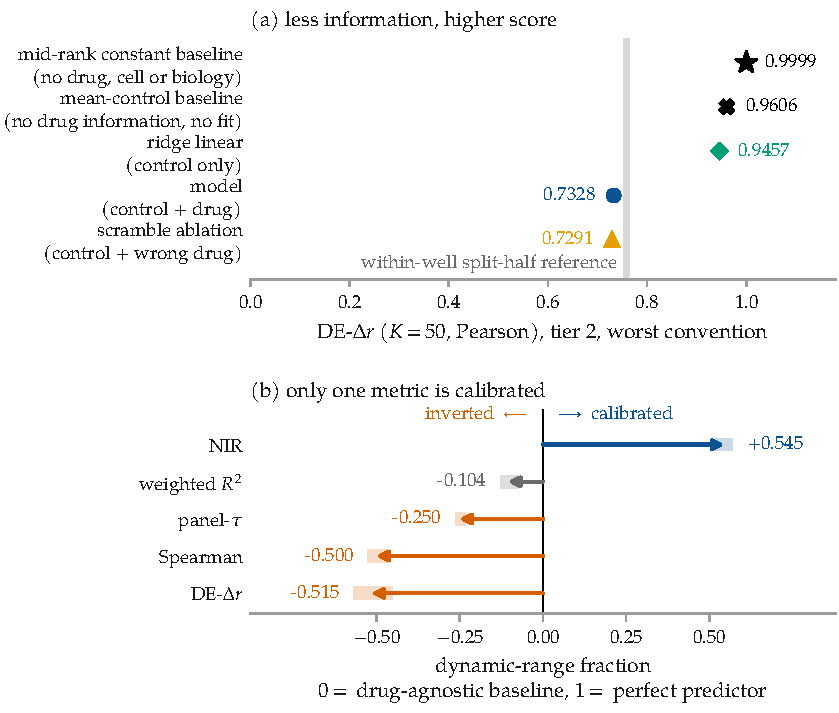
\includegraphics{fig-calibration}
\caption[A zero-information predictor outscores the model]{\textbf{A predictor
carrying nothing about drug, cell or biology scores the field's standard metric
above both the within-well reference and the model, and of five metrics only
$\NIR$ grades in the direction its name implies.} (a) $\DEdr$, $K = 50$,
Pearson, tier 2 unseen drugs, \texttt{worst} convention, $n = 400$ conditions;
the axis runs from $0$ and is not truncated. The grey band marks the within-well
split-half precision reference at $0.76$, the two-real-cell positive control of
\cref{tab:de-artifact}: two halves of the same well, a precision figure and not
a biological replicate. Its width is a drawing device, not an interval, and the
arm marks are bare --- the source carries a normal-approximation interval over
conditions, and this document draws only the clustered bootstrap, so nothing is
drawn rather than an interval of another kind. (b) $\DRF$ for the five metrics
of \cref{tab:drf}, the same-plate arm only: $586$ drugs over $44$
cell-line$\times$plate groups spanning $27$ cell lines, the pale block at each
arrowhead the $95\%$ percentile bootstrap interval clustered on cell line
quoted there.}
\label{fig:calibration}
\end{figure}

\paragraph{What this replicates, and where it does not} The methodological core
of Miller et al.\ replicates, and this audit sharpens it. Metric choice
dominates, and the
control-referenced correlation they flag is the worst performer in both arms
($\DEdr$, $-0.686$ across plates and $-0.515$ within). Their calibrated set does
not transfer intact. \texttt{weighted\_r2}, this project's counterpart of the
weighted $R^2\Delta$~\cite{mejia} they endorse, is negative in both audited
arms, though closest to zero and sign-tracking cell count, so it carries no
directional claim; the inversions of $\paneltau$ and \texttt{spearman\_expr}
belong to neither calibrated set. Their endorsed $\NIR$ does survive. Being
rank-based is not what protects it; refusing to score anything the generic
response can supply is.

\paragraph{Adopting the instrument is also a defence} Miller et al.\ conclude
that under calibrated metrics deep models outperform uninformative baselines;
\cref{sec:res-blind} finds ours at chance on that very
metric.\seealso{\cref{sec:lit-dispute} sets out the dispute this audit enters.}
Genetic against drug perturbation and a discriminative against a generative
model are candidate explanations; \cref{sec:res-lookup} supplies a third.
Adopting their metric also puts the verdict beyond the objections their own
paper raises.

\paragraph{The residual frame is audited separately} A metric is not calibrated
by having a relative calibrated, so the residual frame carries its own
$\DRF$.\framecue{\Rframe}{the second audit is scored in the residual frame,
\cref{sec:methods-residual}} With a split-half replicate as positive control and
the evaluation's drug-agnostic arms as negatives, it reads
\ci{+0.704}{+0.667}{+0.736} against \texttt{control\_copy}, clustered on the
$42$ cell lines. Which negative is chosen barely matters. A random vector and
\texttt{orth} both give $+0.707$, and all three sit at chance as a matter of
measurement ($0.506$, $0.501$, $0.501$). The positive control is the more
conservative of the two, a raw split-half replicate instead of the denoised
interpolated duplicate, so the residual frame is the better separated ($+0.704$
against $+0.635$) despite the harder reference. \texttt{generic} scores exactly
$0.500$ with zero variance, the residual being defined by subtracting it, and
carries no weight.

\paragraph{One declared exception on the intervals} $\DRF$ is a ratio of means;
the two-way estimator used everywhere else here is written for a
mean.\bench{two-way cluster-robust intervals on every
mean}{\cref{sec:methods-data}} Both $\DRF$ intervals are therefore
\emph{one-way} percentile cluster bootstraps that resample whole cell lines and
recompute the ratio inside each draw, respecting the cell-line dependence and
ignoring the crossed well dimension, so they are narrower than fully crossed
intervals. The separation they grade is far too large for that to change the
sign, but the caveat belongs beside the number.

\paragraph{Two questions about the instrument remain, and they differ} The first
is whether the conditions are empirically discriminable at the tested budget. A
spike-in forced choice answers it. Within a plate, a reference pseudobulk from
drug A's cells must be scored closer to a disjoint sample of A's own cells than
to drug B's, chance $0.50$, with contamination of B by A titrating the
difficulty. At zero contamination three of the six metrics run on it
separate the two populations essentially perfectly ($\paneltau = 1.000$,
$\DEdr = 0.995$, top-$n$ $\tau = 0.987$, plate held constant); at full
contamination those same three return $0.501$--$0.502$. The whole-profile
similarities are much weaker even at zero contamination, cosine $0.740$,
Spearman $0.680$, cosine on the shift $0.620$, which matters because a
whole-profile similarity is what $\NIR$ uses here. Split-half retrieval
establishes discriminability, not predictability from untreated input, so
discriminability is not the sole bottleneck at this budget.

The spike-in cannot answer the second question, whether $\NIR$ registers a true
positive, since $\NIR$ was not among the metrics run on it. The evidence is the
$\DRF$ audit's own positive control. Under $\NIR$ the interpolated
duplicate scores $0.802$ against the drug-agnostic mean's $0.457$ across plates,
and $0.668$ against $0.272$ within plate; in the residual frame a split-half
replicate reaches $0.854$ against negatives at $0.501$--$0.506$. None of those is
the reference the verdict is measured against. That reference is the within-well
split-half precision estimate recomputed on the tier-2 within-plate benchmark,
where it sits above chance but not far above it; that, and not $1.0$, is the bar
\cref{sec:res-blind} states the model against.

\begin{scopelimit}[carried into \cref{sec:res-blind} and the rest of the chapter]
The audit licenses $\NIR$ and nothing else. $\paneltau$ is inverted in both
audited arms, so no absolute claim rests on it and no ordering read off it counts
as evidence of skill; an inverted metric preserves neither. Where $\DEdr$
appears later it is only as a paired comparison of two arms on one scale, never
as an absolute score. And a metric is not calibrated by having a relative
calibrated. What is graded here is \texttt{nir\_expr} in the expression frame and
the residual frame's cosine similarity in its own frame, each against its own
controls. A third $\sigma$ would need its own audit.
\end{scopelimit}

\begin{claim}
This audit grades five candidates, and $\NIR$ is the only
one with a positive $\DRF$ (\ci{+0.635}{+0.604}{+0.663} on a one-way cluster
bootstrap over the $25$ cell lines, the declared exception to this chapter's
two-way rule, Holm $p = 0.002$; \ci{+0.545}{+0.516}{+0.569} over $27$ cell lines
with same-plate partners, Holm $p = 0.002$), and the other four are negative with
intervals excluding zero in both audited arms. Three of them ($\paneltau$,
\texttt{spearman\_expr} and $\DEdr$) are inverted rather than merely
uninformative, each ranking the drug-agnostic baseline above the positive
control; \texttt{weighted\_r2} sits closest to zero and its sign tracks cell
count, so no directional claim is made for it. The saturating predictor is not a
curiosity. It carries no information about drug, cell or biology and scores
$\DEdr = 0.9999$ in rank space, above the two-real-cell positive control of
$0.76$ and above the model's $0.73$. Under $\NIR$ the positive control is retrieved well clear of
the negative ($0.802$ against $0.457$ across plates, $0.668$ against $0.272$
within), so the instrument registers a true positive. Every drug-use claim in
the rest of this chapter that rests on a continuous prediction score is
therefore made on the calibrated metric; $\DEdr$ appears below only where two
arms are compared with each other on the same scale, never as an absolute score
of the model's drug use. The remaining instruments (forced-choice grading,
output invariance, and the logit-space activation tests of
\cref{sec:res-mechanism}) are deliberately on scales of their own, each with a
fixed chance value or a paired control.
\end{claim}

% ===========================================================================
% Beat 2.
% ===========================================================================

\beatsection{E}{2}{The model is drug-blind}{sec:res-blind}
\label{sec:methods-controls}   % legacy anchor, so v1 cross-references resolve

\claimlede{On the calibrated metric the model is drug-blind in the expression
frame, including on the identifiable stratum.}

\begin{question}[2]
With a ruler that cannot be gamed in hand, the investigation can ask the
question it exists to answer. Does the model use the drug at all? Four
instruments answer it, and each exists because one specific objection would
otherwise be fatal.
\end{question}

\noindent
The answer is no, and the instruments matter only as the objections they close.
On the calibrated metric, within plate on tier 2 ($n = \num{606}$), the model
scores $0.498$ against a within-well split-half precision reference of
$0.576$.\bench{one estimator,
seven settings}{\cref{tab:ceilings}} It is matched by predictors that know
nothing about the drug: a drug-agnostic linear map scores $0.500$, a
control-copy $0.504$, the global mean $0.180$. And on the identifiable stratum,
whose own within-well reference clears the pre-set $0.80$ bar, a
zero-drug-information control-copy reaches $0.766$ against the model's $0.768$.

\paragraph{Four instruments, and each closes a different objection} The
benchmark itself, within plate; the scramble ablation, the only manipulation
that isolates drug use; forced-choice grading, whose chance value is fixed; and
output invariance, which no scoring choice can confound. They are exposed to
different artefacts, so no single one explains all four.

\paragraph{One measurement rule comes first} Drug and plate are partially
confounded by the atlas's design
(\cref{sec:methods-data}),\framecue{\Eframe}{all four instruments are scored in
the expression frame} so grouping by cell line alone lets the batch effect
stand in for drug identity. A drug-agnostic mean baseline, containing no drug
information whatsoever, scores $0.399$ when the comparison set may span plates
against $0.161$ when it may not, and the precision reference falls from $0.625$
to $0.575$ alongside it, the batch
effect having inflated that too.\seealso{\cref{tab:plateleak} is the leak
audit, a wider run than the benchmark} That is plate leakage, measured and not
assumed. Being wider, its within-plate figures sit slightly off the ones above;
what it licenses is the rule, not a substitute set of scores.

\begin{scopelimit}[carried into every discrimination result in this chapter]
Every discrimination instrument gained a \texttt{--same\_plate\_only} mode and
every discrimination result in this chapter was re-run within plate, except
where a departure from that rule is named at the point of use, as with the
swap-distance sweep that answers the fourth objection below, whose swap partners
were not plate-restricted (\cref{sec:app-sweep}), and the residual-frame scores
of \cref{sec:methods-residual}, whose comparison set is grouped by cell line and
whose justification is given there. Conclusions are unchanged; some magnitudes
shrink.
\end{scopelimit}

\paragraph{The central manipulation is the scramble ablation} The prompt is left
byte-identical except that the drug name and mechanism are replaced by another
drug's, the control cell and the scoring truth unchanged
(\cref{fig:scramble}). Control- and batch-derived leakage therefore cancels in
the scramble gap $\gap = \NIR_{\textrm{model}} - \NIR_{\textrm{scramble}}$, the
only difference in this chapter whose leakage cancels by construction. It does
not displace the drug-agnostic comparisons above and below, which rest on the
within-plate rule instead.

% PLACEMENT ONLY. The float was anchored six paragraphs lower (just before "The
% third instrument"), which is where its [htbp] first became satisfiable -- the
% top of the NEXT page -- and that page then had no room left for
% \cref{tab:blind}, which was pushed a further page past the sentence that
% introduces it (measured: anchor p35, caption p37). Anchoring the figure at the
% paragraph it actually depicts, the scramble ablation itself, is earlier in the
% flow, so the figure takes the top slot one page sooner and the table follows on
% the page after its own anchor. Nothing about the figure or its caption changes.
%
% The paragraph above now carries the \cref, so the anchor is explicit and not
% merely positional. Its second sentence lost the restatement "Both arms share
% the same control cell, so ..." because the figure now sets that clause on one
% unbroken line beneath the two arms; the inference is carried by "therefore"
% off "the control cell ... unchanged" in the sentence before it. No claim,
% hedge or magnitude changed, and the paragraph is one line shorter than it was.
%
% \input, not \includegraphics: figs/fig-scramble.tex is TikZ and carries its
% own float, caption and \label. \input resolves against the main-document
% directory, so this is thesis_v2/figs/, NOT the read-only ../thesis/figs/ that
% \graphicspath adds for raster/PDF assets only.
% ===========================================================================
% fig-scramble.tex (v2) -- the scramble ablation and why its difference is
% leak-immune. NO DATA DEPENDENCY: this is a schematic. The two drug names and
% the two mechanism strings are the illustrative pair already used in v1; the
% only quantity in the float is the definition
% \gap = \NIR_real - \NIR_scrambled, which is the definition given in
% Sections/04a-ruler.tex, not a measurement.
%
% CHANGES FROM v1 (thesis/figs/fig-scramble.tex), all layout, none semantic:
%   (1) the closing sentence is now ONE unbroken line. In v1 it was set as two
%       centred nodes with a dashed arrow BETWEEN them, so the reader crossed a
%       rule in the middle of the clause "so control- and batch-derived /
%       leakage cancels". Measured at \scriptsize the sentence is 360.25pt,
%       which fits the 404.03pt measure with 43.8pt to spare, so the break was
%       never forced -- it existed only to make room for the arrow.
%   (2) the dashed arrow is deleted. It ran left-to-right under the figure and
%       connected nothing: no node at either end, no quantity implied by its
%       direction.
%   (3) the \gap definition is no longer floating in the white between the two
%       curved connectors. It hangs off the LOWER connector on a short vertical
%       tick, so the eye reads "these two arms, differenced" rather than
%       finding a formula parked in open space.
%
% WIDTH. v1 measured 289.4pt = 101.7mm inside a 142mm measure and sat visibly
% short of the block. This version is laid out to 14.2cm = 142.0mm = the v2
% \textwidth (404.03 TeX pt, preamble.tex:88). It is NOT \resizebox'd and it is
% NOT [scale=]'d: every type size below is the size that prints. Widening was
% done by pinning the truth node to the right edge of the block (anchor=east at
% x=14.2) and widening the prompt cards from their natural 3.70cm to 5.60cm, so
% the extra 40mm goes into the converging arms, which is the part of the
% picture that carries the argument, and not into the card interiors.
%
% MEASURED (\settowidth, 12pt Pagella, this preamble):
%   \textwidth                                     404.03pt
%   closing sentence, \scriptsize                  360.25pt   -> one line, fits
%   closing sentence, \footnotesize                450.31pt   -> would not fit
%   prompt tabular, natural                        104.88pt
%   "scrambled prompt --- only the two ..."        192.22pt = 6.78cm
%   \gap definition, \small                        137.96pt
% Those last two set the card width. The cards stop at 5.60cm and the truth
% node starts at 12.09cm, leaving 6.49cm of gap; the 4.86cm \gap definition
% hangs in the middle of that gap with 0.83cm clear on its left and 0.68cm on
% its right, so it touches neither the card nor the truth. A wider card (6.90cm,
% flush with the 6.78cm label above it) was tried and rejected: it squeezed
% those clearances to 3pt and 2pt.
% ===========================================================================
\begin{figure}[htbp]
\centering
\begin{tikzpicture}[
  x=1cm, y=1cm, font=\small,
  lbl/.style={font=\scriptsize, text=quietink},
  strong/.style={font=\scriptsize, text=ink},
  % text width, not minimum width: minimum width would centre the tabular in
  % the enlarged box and the prompt would stop looking like a prompt.
  promptbox/.style={draw=rulegrey, rounded corners=2pt, inner sep=5pt,
                    fill=rulegrey!8, text width=5.248cm, align=left},
  truthbox/.style={draw=rulegrey, rounded corners=2pt, inner sep=6pt,
                   align=center, fill=rulegrey!10},
  ar/.style={-{Stealth[length=4.5pt]}, quietink},
  tick/.style={quietink, line width=0.5pt},
]
% rulegrey!35 reproduces v1's black!14 span shading against the page's own
% rule ink rather than pure black.
\newcommand{\spanhl}[1]{\colorbox{rulegrey!35}{#1}}

% ---- arm 1: the real prompt --------------------------------------------
\node[lbl, anchor=west] at (0,0) {real prompt};
\node[promptbox, anchor=north west] (p1) at (0,-0.26) {%
  \renewcommand{\arraystretch}{0.9}%
  \begin{tabular}{@{}l@{~~}l@{}}
  \ttfamily\scriptsize Cell line:    & \ttfamily\scriptsize MCF7 \\
  \ttfamily\scriptsize Drug:         & \ttfamily\scriptsize \spanhl{Lapatinib} \\
  \ttfamily\scriptsize Mechanism:    & \ttfamily\scriptsize \spanhl{EGFR inhibitor} \\
  \ttfamily\scriptsize Control cell: & \ttfamily\scriptsize ACTB GAPDH \ldots \\
  \end{tabular}};

% ---- arm 2: the scramble. Positioned OFF p1's measured south edge, never off
% an estimate of the card height -- the card is ~2.2cm tall once the shaded
% spans are set, which is more than four lines of \scriptsize looks like it
% should need.
\node[lbl, anchor=north west] (l2) at ($(p1.south west)+(0,-0.34)$)
  {scrambled prompt --- only the two shaded spans differ};
\node[promptbox, anchor=north west] (p2) at ($(l2.south west)+(0,-0.10)$) {%
  \renewcommand{\arraystretch}{0.9}%
  \begin{tabular}{@{}l@{~~}l@{}}
  \ttfamily\scriptsize Cell line:    & \ttfamily\scriptsize MCF7 \\
  \ttfamily\scriptsize Drug:         & \ttfamily\scriptsize \spanhl{Vorinostat} \\
  \ttfamily\scriptsize Mechanism:    & \ttfamily\scriptsize \spanhl{HDAC inhibitor} \\
  \ttfamily\scriptsize Control cell: & \ttfamily\scriptsize ACTB GAPDH \ldots \\
  \end{tabular}};

% ---- the single truth, on the right edge of the measure -----------------
% anchor=east at x=14.2 pins the picture's right edge to \textwidth exactly.
\coordinate (mid) at ($(p1.east)!0.5!(p2.east)$);
\node[truthbox, anchor=east] (truth) at (14.2,0 |- mid)
  {truth for\\\textbf{Lapatinib}\\{\scriptsize drawn once}};

% Both arms leave horizontally and arrive on the truth from the outside, so
% the convergence is the shape of the picture.
\draw[ar] (p1.east)
  .. controls ($(p1.east)+(2.7,0)$) and ($(truth.north west)+(-1.0,0.30)$)
  .. (truth.north west);
\draw[ar] (p2.east)
  .. controls ($(p2.east)+(2.7,0)$) and ($(truth.south west)+(-1.0,-0.30)$)
  .. (truth.south west) coordinate[pos=0.42] (hang);

% ---- the definition, hung off the lower connector ----------------------
\draw[tick] (hang) -- ($(hang)+(0,-0.62)$);
\node[anchor=north, font=\small, inner sep=1pt] (gapdef) at ($(hang)+(0,-0.62)$)
  {$\gap = \NIR_{\text{real}} - \NIR_{\text{scrambled}}$};

% ---- the reason the difference is leak-immune, on one line -------------
\node[strong, anchor=north] at (7.1,-6.00)
  {the shared control cell enters \emph{both} arms, so control- and
   batch-derived leakage cancels in the difference};

\end{tikzpicture}
\caption[The scramble ablation]{\textbf{The scramble replaces the drug name and its mechanism and
nothing else.} Both arms are conditioned on the same control cell and scored against the same truth,
so any leakage through the control cell or the plate enters both arms in equal measure and cancels in
the difference $\gap$. This is why $\gap$ is the only difference in the chapter whose leakage cancels
by construction, while a comparison against a drug-agnostic predictor is not leak-immune --- such a
baseline inherits whatever plate structure the comparison set carries
(Table~\ref{tab:plateleak}). Comparisons of that kind are used, and used centrally, with the
comparison set declared at every score: within plate in the expression frame, where the leakage is
controlled rather than cancelled, and by cell line in the residual frame, where the plate-scoped
generic has already subtracted each plate's mean response from truths and predictions alike --- in
expectation, with however much survives in an individual residual left unmeasured
(\S\ref{sec:methods-residual}, and \S\ref{sec:limitations} for what that leaves open).
A refinement matters here: if the swapped-in drug happens to have a
\emph{similar} true response then an unchanged output is correct rather than blind, so the swap
partner is chosen from three defined similarity strata by residual cosine. Which stratum can carry
the canonical magnitude associated with this figure is constrained by the comparator's own score.
\S\ref{sec:res-generalisation} finds the geometry-defined \texttt{orth} partner empirically near
chance at $0.501$ in this sample, making it the least contaminated available comparator rather than
an independently established null. That restriction belongs to this canonical scramble comparison:
the three-stratum repair comparison differences each model score against its own
\texttt{near}/\texttt{orth}/\texttt{opposite} partner, while field attribution uses its stated
span-specific partner and retains the resulting comparator caveat.}
\label{fig:scramble}
\end{figure}


% fig:comparator sits here, two paragraphs above the sentence that cites it,
% because both floats then queue from the same point and LaTeX keeps them in
% order: fig:scramble takes the next top slot and fig:comparator the one after,
% which lands it on the spread that carries the stratified-scramble paragraph.
% It is cited here and used in full six sections later (sec:res-generalisation);
% placing it there instead would put the picture of what the strata are three
% chapters' worth of pages after the paragraph that defines them. Its caption
% carries the forward pointer, so the reader who meets it early is told where
% the argument is finished. Same \input rule as above: figs/fig-comparator.tex
% carries the float, caption and \label, and reads fig-comparator.pdf out of
% thesis_v2/figs/.
% fig-comparator.tex -- float wrapper for fig:comparator.
% Data: thesis_v2/figs/fig-comparator.json, written by thesis_v2/figs/comparator.py from
% RESULTS_cluster/scramble_stratum_audit_v4.json and RESULTS_cluster/re_v3.json.
% Placement: Sections/04a-ruler.tex, immediately after \input of fig-scramble.
% NO width= KEY. The PDF is drawn at 142mm, which is exactly \linewidth in the body block, so
% \includegraphics{} places it at 1.0 and the 10pt type in it prints at 10pt. Adding
% [width=\linewidth] would be harmless today and a silent 11% type shrink the moment the measure
% changes; \resizebox would be wrong at any measure.
\begin{figure}[htbp]
\centering
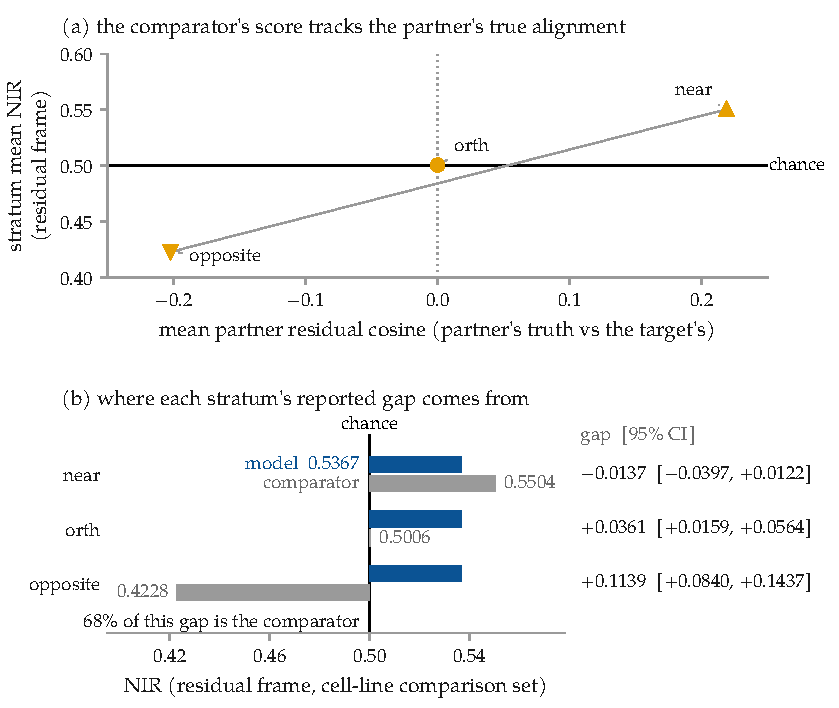
\includegraphics{fig-comparator}
% Short caption: 46 characters, and it states the finding rather than the topic. The long form
% below carries the calibration half of the argument; the List of Figures gets the consequence.
\caption[Most of the \texttt{opposite} gap is the comparator]{%
\textbf{The comparator's own score is a monotone function of how correct the swapped-in partner
is, so most of the \texttt{opposite} stratum's headline gap is the comparator failing rather than
the model knowing.} All quantities are residual-frame $\NIR$ scored against the cell-line
comparison set, pooled over the $\num{1394}$ scored conditions.
\emph{(a)} Each mark is one swap stratum, at its mean partner residual cosine and its mean
$\NIR$. The score falls from $0.5504$ through $0.5006$ to $0.4228$ as the partner's true residual
moves from aligned to anti-aligned, so \texttt{near} hands the model a partly correct answer and
\texttt{opposite} an actively wrong one. The straight line is the chord joining the two extreme
marks, drawn as a guide to the eye; it is not a fit, and \texttt{orth} lies $0.016$ above it.
Because the strata are defined using the \emph{true} residual geometry, \texttt{orth}'s sitting on
chance is an empirical property of this sample and not an independently established null: it is
the least contaminated comparator available, which is a weaker statement
(\cref{sec:res-generalisation}).
\emph{(b)} The same gap $\gap$ split at chance into its two terms,
$\gap = (\NIR_{\textrm{model}} - 0.5) + (0.5 - \NIR_{\textrm{scramble}})$. The accent bar is the
model's own advantage over chance, $+0.0367$, and is identical on all three rows because it is the
same model arm; the strata differ only in the grey bar, the comparator's own displacement from
chance, drawn on the side it actually falls --- right of the rule it subtracts from the gap, left
of the rule it adds. On \texttt{opposite} the grey term is $+0.0772$ of the $+0.1139$ reported,
$68\%$ of it, which is the annotation on that row.
Intervals are $95\%$ two-way cluster-robust on cell line and treatment well ($42$ cell lines,
$200$ wells); the one-way variants stored alongside them are not drawn.}
\label{fig:comparator}
\end{figure}


\paragraph{Two constraints on the swap partner} The partner must be a different
drug. Allowing the same drug at another dose or plate substitutes the drug for
itself, an unchanged prediction is then correct and not blind, and the contamination
concentrates in the most similar stratum. It must also be on the same plate,
since residuals retain plate structure and a cross-plate partner would differ in
batch as well as in drug.

A scramble that swaps in a drug with a similar true response is a weak test, and
that risk is structural here. In full-profile space the mechanism annotation is
close to uninformative about transcriptional response. Same-mechanism drugs in
Tahoe are just over two per cent closer to each other than arbitrary pairs
are.\seealso{\cref{sec:res-encoding} quotes the distances behind that statement}
Hence conditioning on mechanism fails to move $\DEdr$ in the grouping ladder of
\cref{sec:res-lookup}, and a partner of different mechanism cannot be relied on
for a different response. Mechanism does carry signal in the residual frame
(\cref{sec:res-scope}); in full-profile space the generic response swamps it, a
frame difference and not a contradiction.

Two remedies are used. A swap-distance sweep bins (drug, swap) pairs by the
response distance $\lVert y_A - y_B \rVert$ between real and swapped-in drug,
turning the single test into a curve (\cref{sec:app-sweep}). And a stratified
scramble defines three partners per condition by residual cosine within the cell
line: \texttt{near} (most similar), \texttt{orth} ($\cos\approx0$) and
\texttt{opposite} (most anti-correlated). The strata expose what a single
comparator hides (\cref{fig:comparator}): the gap it defines has two parts, how
much naming the truth helps and how much naming a lie hurts, and only the first
is wanted, so a usable null is a stratum scoring at chance.
\Cref{sec:res-generalisation} shows exactly one qualifies, and not the one an
evaluation would default to.

\paragraph{The third instrument is forced-choice grading} A prediction is scored
against its own condition's truth and against another drug's truth from the same
comparison set, recording how often its own wins. Chance is $0.50$ by
construction, and the precision reference lands between $0.67$ and $0.83$
depending on cells per condition.

\paragraph{The fourth is output invariance} It asks whether the drug token
changes the generated text at all, without reference to any truth. It is run at
$3800$ tokens, the longest budget in the chapter, because
truncation would cut the comparison
itself.\seealso{\cref{sec:methods-data} records the four generation budgets} For
a fixed control cell it compares
% \resizebox, not a reflow: the two \underbrace labels are the width, and both
% are wanted on one line so the subtraction reads as one sentence. Natural
% width is 165.6mm against the 142mm block (67.15pt over), so this sets at
% about 0.86. Nothing here is body text.
\begin{equation}
\resizebox{\linewidth}{!}{$\displaystyle
 \textrm{invariance gap} \;=\;
 \underbrace{\overline{\textrm{sim}}(\textrm{same prompt, resampled})}%
   _{\textrm{sampling noise alone}}
 \;-\; \underbrace{\overline{\textrm{sim}}(\textrm{prompts differing in the
   drug})}_{\textrm{noise plus any drug effect}},
$}
\end{equation}
with similarity as top-$100$ Kendall $\tau$ and as Jaccard overlap, over $8$
contexts $\times$ $12$ drugs at temperature $0.8$. It is the least informative
of the four and the least confoundable.

\begin{table}[htbp]
\begin{fullwidth}
\begin{threeparttable}
\caption{\textbf{Four independent instruments agree, and the two that return
intervals bound the drug's effect instead of merely covering zero.} Near-ceiling
$\DEdr$ is achieved identically with a wrong-mechanism drug, so that score is
drug-independent.}
\label{tab:blind}
\small
% Column 3 was `l'. At the widened measure its natural width ("$0.48$
% ($\approx$ scramble; reference 0.67--0.83)") plus columns 1--2 left the X
% column too narrow for the single unbreakable word "indistinguishable", which
% ran 43.91pt past the fullwidth block. Column 3 is now a weighted X so it
% wraps; the two \hsize factors sum to 2, which is what tabularx requires of
% two X columns.
\begin{tabularx}{\linewidth}{@{}l l
  >{\hsize=1.20\hsize\raggedright\arraybackslash}X
  >{\hsize=0.80\hsize\raggedright\arraybackslash}X@{}}
\toprule
\thead{Instrument} & \thead{Quantity} & \thead{Value} & \thead{Reading} \\
\midrule
Forced-choice grading & own-truth win rate
  & $0.48$ ($\approx$ scramble; reference 0.67--0.83) & chance \\
Output invariance & invariance gap & \ci{0.000}{-0.019}{+0.016}
  & bounded, $\leq 0.016$ \\
\addlinespace
Scramble, tier 1 & $\DEdr$ & $0.740$ real vs $0.739$ scrambled
  & indistinguishable \\
Scramble, tier 2 & $\DEdr$ & $0.733$ real vs $0.729$ scrambled
  & indistinguishable \\
Scramble (identifiable subset) & $\gap$ ($\NIR$) & \ci{+0.014}{-0.016}{+0.042}
  & bounded, $\leq +0.042$ \\
\bottomrule
\end{tabularx}
\begin{tablenotes}[flushleft]\footnotesize
\item The two $\DEdr$ rows are paired comparisons on one scale, the only use
\cref{sec:res-metrics} licenses for that metric.
\end{tablenotes}
\end{threeparttable}
\end{fullwidth}
\end{table}

% PLACEMENT ONLY. This is one of the three survivors the \paragraph orphan patch
% in preamble.tex section 4 records: the global reservation is
% 3\baselineskip, which this head cleared with 2.3 lines to spare and then set
% itself plus exactly two lines at the foot of the page. 5 lines is head plus
% four, which the page cannot fake.
\needspace{5\baselineskip}%
\paragraph{An interval that covers zero earns its keep by what it excludes} Not
by the word \emph{null}. Two predictions from a byte-identical prompt agree at
$\tau = 0.198$, so the invariance interval caps any drug-driven divergence at
roughly a twelfth of that agreement, and the Jaccard version is tighter still,
\ci{+0.000}{-0.008}{+0.008}. On the identifiable stratum the scramble gap of
\ci{+0.014}{-0.016}{+0.042} runs against the $0.170$ separating the model's
$0.768$ from that stratum's $0.938$ reference; at the very top of the interval,
naming the right drug would buy a quarter of what is there to be bought, and the
point estimate puts it at $8\%$ of that. Neither figure shows the effect is
zero, and no experiment here could. Both put it far below the headroom these
conditions leave.

\paragraph{Four objections close on measurement, not argument} The first is
whether there is anything to know at all. A ladder of mean-shift baselines
answers it, and the informative conditioning variable is the cellular context,
not the drug class.\seealso{\cref{sec:res-lookup} gives the ladder}

The second decides whether this section reports a result or an instrument
failure. Barely half the atlas clears the pre-set identifiability bar
(\cref{tab:scale}), so the verdict is re-scored where the wells are demonstrably
adequate. That does not rescue the model. It appears to beat the linear baseline
there ($0.768$ against $0.531$), yet a zero-drug-information control-copy
reaches $0.766$ on the same conditions, the paired contrast is
\ci{+0.002}{-0.026}{+0.028}, and the leak-immune $\gap$ stays bounded as above.

The control arm carries a second result that is easy to walk past. Across the
three strata its score tracks the reference almost step for step
(\cref{fig:difficulty}, panel b): $0.310$
against a reference of $0.287$ on the low-reference stratum, $0.540$ against
$0.689$ on the marginal one, $0.766$ against $0.938$ on the identifiable one. A
predictor knowing nothing whatever about any drug does best exactly where the
ranking problem is easiest, so what makes a condition identifiable is largely
what makes its untreated cells distinctive among their plate-mates, and the
distance to a high reference is not all room that better drug modelling would
fill. The reference rises with aggregation (\cref{fig:difficulty}, panel a:
$0.61$ at $10$ cells, $0.76$
at $40$, $0.85$ at $120$); what the strata add is that most of the ranking can
be done without the drug.

\begin{figure}[htbp]
\centering
% drawn at 142mm by thesis_v2/figs/difficulty.py; no width= key, so it is placed
% at scale 1.0 and its type prints at the point sizes it was set in.
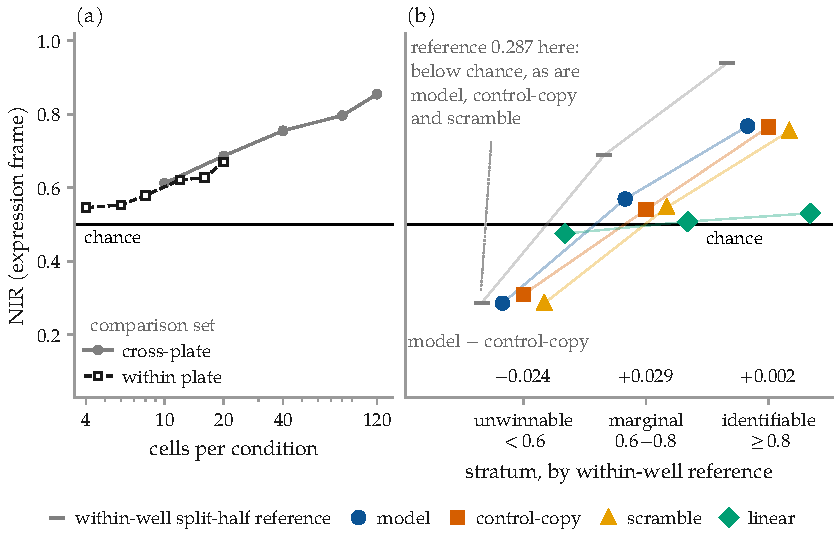
\includegraphics{fig-difficulty}
\caption[Difficulty structure and the stratum ladder]{\textbf{Conditions are
more empirically discriminable at the tested pseudobulk budget where the
precision reference is high, and precisely there, a predictor containing no drug
information matches the model.} Both panels are $\NIR$ in the expression frame,
on one shared axis. (a) The within-well split-half precision reference against
cells per condition, for two comparison sets: cross-plate, and within plate. (b)
The same reference used to bin conditions, five arms per stratum, $n = 296$
unwinnable, $106$ marginal, $204$ identifiable. On the unwinnable stratum the
reference itself is $0.287$, below chance, as are the model, control-copy and
scramble marks. On the identifiable stratum the model reaches $0.768$ and a
control-copy baseline $0.766$, paired contrast \ci{+0.002}{-0.026}{+0.028},
clustered over cell lines. Plotting the model alone would suggest it does better
on higher-reference drugs. The arm marks are bare: the source carries no
interval for a stratum mean, and this document draws only the clustered
bootstrap, so nothing is drawn rather than an interval of another kind.}
\label{fig:difficulty}
\end{figure}

The third objection is whether the representation throws the drug away. Cell
sentences keep only the rank order of genes and discard expression magnitude; if
the drug lived there the following sections would attack the wrong thing. It is
testable without any model, by asking whether true expression discriminates
drugs better than rank does, and it does not.\seealso{\cref{sec:res-lookup}
gives that measurement}

The fourth is whether the scramble swaps in similar drugs. The swap-distance
sweep bounds this rather than settling it, and it sits outside the within-plate
rule, being an earlier run at \texttt{max\_new\_tokens=1200} scored on the
unseen-drug tier of a different evaluation set, with swap partners not
plate-restricted, and with $n=40$ per bin wide enough to exclude a large effect
but not to establish a null (\cref{sec:app-sweep}). Neither column has an
interval excluding zero in any distance bin; in the single-cell column the far
tail reads $-0.019$ across a $2.3\times$ spread in swap distance, trend
correlation $+0.051$. That column bounds a large dissimilarity effect for the
expression-frame model. The optimal-transport column cannot, since
\cref{sec:res-encoding} later shows that checkpoint clears zero under the
canonical within-plate stratified test at the matched
\texttt{max\_new\_tokens=1400} budget. Its apparent null is budget-dependent,
and the stratified scramble replaced the sweep in the reported set.

\begin{claim}
The model is at chance overall ($0.498$ against a $0.576$ within-well split-half
precision reference), matched on the identifiable stratum by a
zero-drug-information control-copy ($0.768$ against $0.766$, paired contrast
\ci{+0.002}{-0.026}{+0.028}), and no more moved by a maximally dissimilar swap
than by a similar one in the single-cell column of a non-canonical
\texttt{max\_new\_tokens=1200} sweep outside the within-plate rule
(\cref{sec:app-sweep}). The sweep's optimal-transport column does not carry that
bound; \cref{sec:res-encoding} later shows the same checkpoint is non-null under
the canonical test at the matched $1400$-token budget.
\end{claim}

% ===========================================================================
% 04b-representation.tex -- beats 3-4. The expression frame, read in the weights.
% Source: thesis/Sections/Investigation-v4.tex 1052-1545.
% Every number, interval, n and conclusion is verbatim from v1.
%
% Consistency pass: the section now opens by naming the third question of
% \cref{sec:intro-map} and stating its answer -- identity written into the
% activations, barely consulted by generation -- before the instruments, so a
% reader arriving from the introduction finds what was promised. The stratum
% paragraph and its \scopelimit are adjacent again, since the scope limit is
% about that stratum's reference. "Step three, the removal gate" was a \defn
% box between three \paragraph steps; it is now the paragraph it always was,
% merged with the gate result that followed it. Vocabulary: "output" as a noun
% for the prediction, "compound", and bare "signature" are gone; "shift" is
% reserved for treated minus control, so the logsumexp constant is an offset.
% ===========================================================================

% ===========================================================================
\beatsection{E}{3}{The drug is not missing from the computation}{sec:methods-probe}

\begin{question}[3]
A model that ignores a drug it was told about can fail in two ways. Either the
drug never enters its computation, an activation-side encoding failure that
target- and input-side fixes might reach, or it enters and nothing reads it, a
decoder failure only an objective-side fix could reach. Behaviour cannot tell
them apart, since both predict the same scores. The weights can. A linear decode
probe, read as a floor test and not as evidence of use, settles the first half.
\end{question}

\noindent
\Cref{sec:intro-map} asks where useful prediction fails: is the drug absent from
the data, lost from the model's representation, or encoded and underused by
generation? The three sections that follow answer in one direction, and the
answer is worth having before the instruments. Drug identity is written into the
activations and stays written, more legibly with depth once batch structure is
projected out, while generation consults it too weakly to account for the
drug-blindness of \cref{sec:res-blind}. The failure is not on the activation
side. Neither half comes free: the presence result is close to guaranteed by
construction, the low-gain reading rests on the weakest measurement in the
chapter, and both are carried below with the discount attached.

Every behavioural measurement so far fits the last two readings
equally.\framecue{\Eframe}{scores here are full-profile, \cref{sec:res-metrics}}
\Cref{sec:res-blind} has answered the first where it matters here: the task is
empirically discriminable for a substantial stratum at the tested pseudobulk
budget, the reference rises with aggregation, $46.2\%$ of conditions clear the
declared identifiability bar, and on those the model is matched exactly by a
baseline copying the untreated cell ($0.768$ against $0.766$).\gloss{identifiable
stratum}{conditions whose own within-well split-half reference clears the pre-set
bar} The shortfall there is the model's; where in the model it lives needs the
weights.

\begin{scopelimit}[carried into \cref{sec:res-epsilon} and \cref{sec:limitations}]
The distance from a score to that stratum's reference is not available headroom.
Across the three difficulty strata of \cref{sec:res-blind} the control-copy's own
score tracks the reference almost step for step: $0.310$ against a reference of
$0.287$ on the low-reference stratum, $0.540$ against $0.689$ on the marginal one,
and $0.766$ against $0.938$ on the identifiable one. A predictor that reproduces
the untreated cell and knows nothing whatever about any drug does best exactly
where the ranking problem is easiest. What separates the strata on this
criterion is largely drug-independent: within a comparison set every condition's
untreated cells come from one plate-matched DMSO pool, so a control-copy scores
high exactly where a condition's measured profile sits closer to that shared
untreated state than its plate-mates' do. Most of the ranking these conditions
are scored on can therefore be done without the drug, and the gap between a predictor and a high reference is
not all of it room that better drug modelling would fill. Every score quoted on
the identifiable stratum below inherits that reading, including the three target
constructions of \cref{sec:res-epsilon}.
\end{scopelimit}

\paragraph{Three sub-questions, in the order their blind spots close} Is drug
identity present in the activations? Does the network use the region where it is
written? And does it use \emph{which} drug? Each instrument's blind spot is what
the next must close; \cref{sec:res-epsilon} adds a fourth.
\Cref{fig:comparators} maps all four, on scales that may not be read across.

% ===========================================================================
\begin{figure}[htbp]
\begin{fullwidth}
\centering
% ===========================================================================
% figs/comparators.tex -- fig:comparators, reworked for thesis_v2.
% FIGURE BODY ONLY. No preamble, no document environment. \input it from
% inside a figure/fullwidth float in Sections/04b-representation.tex.
%
% Four instruments, four deliberately incommensurable value-to-position maps,
% one comparator each. The premise and all four scales are v1's and unchanged.
% What changed is labelling only; no mark moved, no number changed.
%
%   (1) ROW B plotted seven marks and named one ("all seven layers"), leaving
%       six unidentifiable. Every mark is now named by the layer it is, with a
%       fanned leader for the three that crowd at 3.6/3.8/4.2, and the stub
%       carries "one mark per layer" so a bare accent numeral above the axis
%       cannot be misread as a second set of tick labels (ticks are quietink
%       and below the axis; layer numbers are accent and above it).
%   (2) ROW A's "slab projected out" sat to the right of its own point and
%       nearer the shuffled-label rule than to the mark it names. It now has a
%       leader back to the 0.121 dot.
%   (3) ROW C's single-cell marker was a hollow ring sitting on the dotted zero
%       rule (-0.0012 against 0.000: 0.10cm apart on this scale). It is now
%       solid, the zero rule is interrupted across its height so nothing runs
%       into it, and its label starts 0.30cm clear with a leader through the
%       interruption -- necessary because the zero rule lies between mark and
%       label and would otherwise claim the label.
%   (4) Bar labels in ROWS C and D moved from a 0.13cm to a 0.30cm gap, so
%       "optimal-transport barycentric" no longer reads as a continuation of
%       its own interval bar.
%   General rule applied throughout: a label more than ~0.3cm from its mark
%   gets a short leader.
%   Row heights grew (rows now 0.70/0.77/0.98 apart rather than colliding) to
%   pay for the new labels. Nothing is rescaled: 1cm here is 1cm on the page.
%
% PROVENANCE of every number drawn is in comparators.json, sibling to this
% file. All four rows were checked against RESULTS_cluster and against the
% thesis text; they agree. Sources:
%   row A, B  RESULTS_cluster/workspace_probe.json
%   row C     RESULTS_cluster/probe_arm_residual.json,
%             probe_rep_residual_s43.json, probe_rep_residual_s45.json,
%             probe_arm_single_cell.json
%   row D     RESULTS_cluster/stratify_sameplate_final.json,
%             stratify_ot_T2.json, stratify_consensus.json
% ===========================================================================
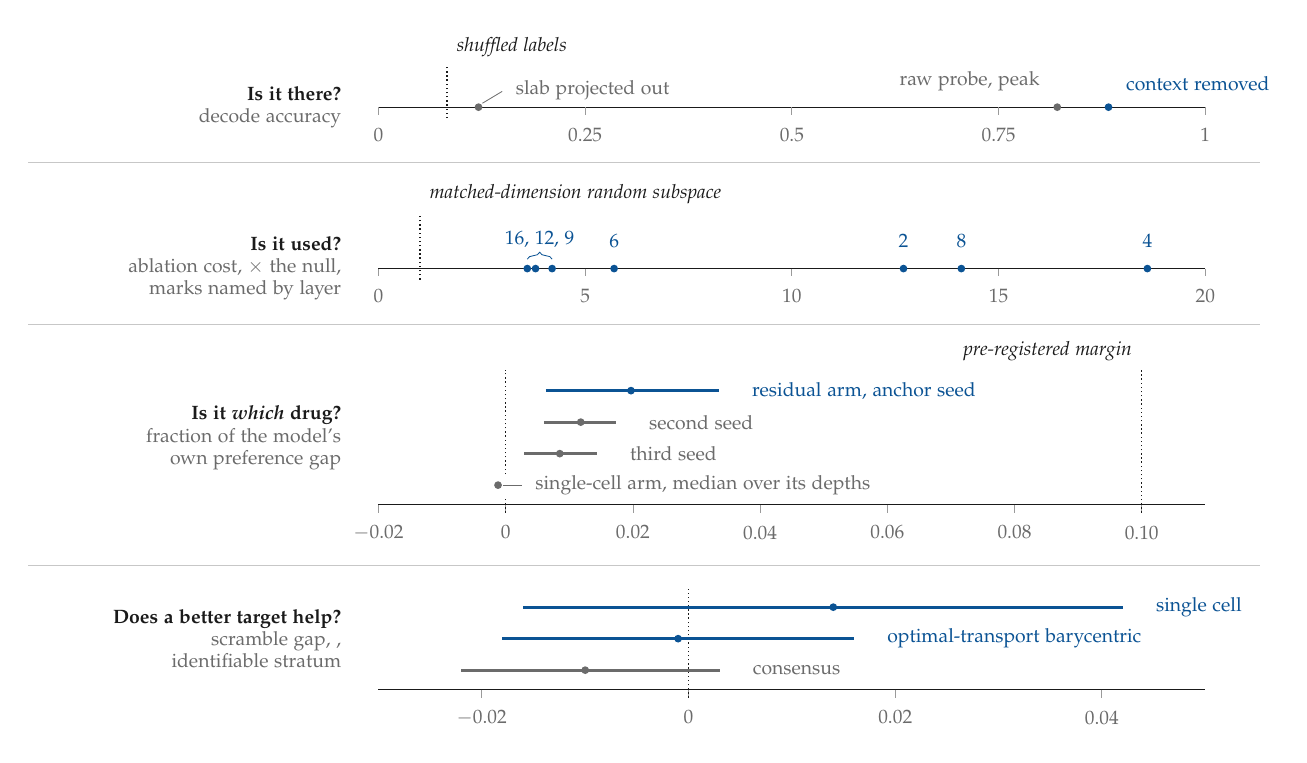
\begin{tikzpicture}[x=1cm, y=1cm, font=\small]
  % Four deliberately different value-to-position maps, one per rule.
  \def\xa#1{{(#1)*10.5}}
  \def\xb#1{{(#1)/20*10.5}}
  \def\xc#1{{((#1)+0.02)/0.13*10.5}}
  \def\xd#1{{((#1)+0.03)/0.08*10.5}}
  % Same maps shifted by a label gap; the shift MUST sit inside the braces --
  % \xa{v}+0.05 is not a pgfmath expression and does not compile.
  % 0.30cm, not v1's 0.13cm: at 0.13cm a label abutted the end of its own
  % interval bar and read as part of it.
  \def\xcR#1{{((#1)+0.02)/0.13*10.5+0.30}}
  \def\xdR#1{{((#1)+0.03)/0.08*10.5+0.30}}
  % leader/label shims: +0.05 and +0.06 clear a 1.4pt marker, -0.10 and +0.10
  % keep row A's two abutting labels off their own dots, +0.35 puts row C's
  % single-cell label 0.30cm clear of the marker's edge.
  \def\xaN#1{{(#1)*10.5+0.05}}
  \def\xaL#1{{(#1)*10.5-0.10}}
  \def\xaP#1{{(#1)*10.5+0.10}}
  \def\xcN#1{{((#1)+0.02)/0.13*10.5+0.06}}
  \def\xcM#1{{((#1)+0.02)/0.13*10.5+0.35}}

  % row dividers
  \foreach \y in {-0.70,-2.76,-5.82}{
    \draw[rulegrey!55, line width=0.3pt] (-4.45,\y) -- (11.20,\y);}

  % ===== ROW A -- is it there? decode accuracy, 0 to 1 ====================
  \draw[ink, line width=0.4pt] (0,0) -- (10.5,0);
  \foreach \v in {0,0.25,0.5,0.75,1}{
    \draw[rulegrey, line width=0.3pt] (\xa{\v},0) -- (\xa{\v},-0.10);
    \node[anchor=north, font=\scriptsize, text=quietink] at (\xa{\v},-0.14) {\v};}
  \draw[ink, line width=0.5pt, densely dotted] (\xa{0.083},-0.14) -- (\xa{0.083},0.52);
  \node[anchor=south west, font=\scriptsize\itshape, text=ink]
    at (\xa{0.083},0.52) {shuffled labels};
  % 0.121 -- the constant post-ablation floor. Its label is pushed clear of the
  % shuffled-label rule 0.40cm to its left and leadered back to the mark.
  \fill[quietink] (\xa{0.121},0) circle (1.4pt);
  \draw[quietink, line width=0.3pt] (\xaN{0.121},0.05) -- (1.57,0.20);
  \node[anchor=west, font=\scriptsize, text=quietink]
    at (1.62,0.22) {slab projected out};
  \fill[quietink] (\xa{0.821},0) circle (1.4pt);
  \node[anchor=south east, font=\scriptsize, text=quietink]
    at (\xaL{0.821},0.08) {raw probe, peak};
  \fill[accent] (\xa{0.883},0) circle (1.4pt);
  \node[anchor=south west, font=\scriptsize, text=accent]
    at (\xaP{0.883},0.08) {context removed};
  \node[anchor=east, align=right, font=\scriptsize, text=ink] at (-0.35,0)
    {\textbf{Is it there?}\\ \textcolor{quietink}{decode accuracy}};

  % ===== ROW B -- is it used? ablation cost in multiples of the null =======
  \draw[ink, line width=0.4pt] (0,-2.05) -- (10.5,-2.05);
  \foreach \v in {0,5,10,15,20}{
    \draw[rulegrey, line width=0.3pt] (\xb{\v},-2.05) -- (\xb{\v},-2.15);
    \node[anchor=north, font=\scriptsize, text=quietink] at (\xb{\v},-2.19) {\v};}
  \draw[ink, line width=0.5pt, densely dotted] (\xb{1},-2.19) -- (\xb{1},-1.35);
  \node[anchor=south west, font=\scriptsize\itshape, text=ink]
    at (\xb{1},-1.35) {matched-dimension random subspace};
  % Seven marks, one per layer, and every mark is named. Four are named
  % directly. The other three are layers 16, 12 and 9, reading 3.6, 3.8 and
  % 4.2: 1.1mm and 2.2mm apart on this axis. Three separate leaders into that
  % converge and stop being readable, and fanning them wide enough to separate
  % would claim a resolution the marks do not have, so the cluster is braced
  % and named as an ordered set instead. Reading order is the axis order.
  \foreach \v in {3.6,3.8,4.2,5.7,12.7,14.1,18.6}{
    \fill[accent] (\xb{\v},-2.05) circle (1.4pt);}
  \draw[accent, line width=0.3pt, decorate,
        decoration={brace, amplitude=2.5pt}] (\xb{3.6},-1.93) -- (\xb{4.2},-1.93);
  \node[anchor=south, font=\scriptsize, text=accent, inner sep=1pt]
    at (\xb{3.9},-1.83) {16, 12, 9};
  \foreach \x/\lay in {5.7/6, 12.7/2, 14.1/8, 18.6/4}{
    \node[anchor=south, font=\scriptsize, text=accent, inner sep=1pt]
      at (\xb{\x},-1.83) {\lay};}
  \node[anchor=east, align=right, font=\scriptsize, text=ink] at (-0.35,-2.05)
    {\textbf{Is it used?}\\
     \textcolor{quietink}{ablation cost, $\times$ the null,}\\
     \textcolor{quietink}{marks named by layer}};

  % ===== ROW C -- is it WHICH drug? fraction of the model's own gap ========
  \draw[ink, line width=0.4pt] (0,-5.05) -- (10.5,-5.05);
  % The label is carried separately from the coordinate so the negative tick
  % sets a real minus and not the ASCII hyphen \foreach would print. Same idiom
  % as gate.tex and power.tex; positives stay unmathed so their digits match
  % rows A and B, which are set in text.
  \foreach \v/\t in {-0.02/$-0.02$, 0/0, 0.02/0.02, 0.04/0.04, 0.06/0.06,
                     0.08/0.08, 0.10/0.10}{
    \draw[rulegrey, line width=0.3pt] (\xc{\v},-5.05) -- (\xc{\v},-5.15);
    \node[anchor=north, font=\scriptsize, text=quietink] at (\xc{\v},-5.19) {\t};}
  % The zero rule is drawn in two pieces. The single-cell median sits at
  % -0.0012, one tenth of a centimetre from zero on this scale, so the rule is
  % interrupted across the marker's height rather than run through it.
  \draw[ink, line width=0.5pt, densely dotted] (\xc{0},-5.15) -- (\xc{0},-4.94);
  \draw[ink, line width=0.5pt, densely dotted] (\xc{0},-4.66) -- (\xc{0},-3.34);
  \draw[ink, line width=0.5pt, densely dotted] (\xc{0.10},-5.15) -- (\xc{0.10},-3.34);
  \node[anchor=south east, font=\scriptsize\itshape, text=ink]
    at (\xc{0.10},-3.34) {pre-registered margin};
  \draw[accent, line width=1.0pt] (\xc{0.0063},-3.60) -- (\xc{0.0335},-3.60);
  \fill[accent] (\xc{0.0197},-3.60) circle (1.4pt);
  \node[anchor=west, font=\scriptsize, text=accent] at (\xcR{0.0335},-3.60)
    {residual arm, anchor seed};
  \draw[quietink, line width=1.0pt] (\xc{0.0060},-4.00) -- (\xc{0.0173},-4.00);
  \fill[quietink] (\xc{0.0118},-4.00) circle (1.4pt);
  \node[anchor=west, font=\scriptsize, text=quietink] at (\xcR{0.0173},-4.00)
    {second seed};
  \draw[quietink, line width=1.0pt] (\xc{0.0029},-4.40) -- (\xc{0.0143},-4.40);
  \fill[quietink] (\xc{0.0085},-4.40) circle (1.4pt);
  \node[anchor=west, font=\scriptsize, text=quietink] at (\xcR{0.0143},-4.40)
    {third seed};
  % Solid, like every other point mark; the absent bar is what says it carries
  % no interval. Leader crosses the interruption in the zero rule.
  \fill[quietink] (\xc{-0.0012},-4.80) circle (1.4pt);
  \draw[quietink, line width=0.3pt] (\xcN{-0.0012},-4.80) -- (\xcR{-0.0012},-4.80);
  \node[anchor=west, font=\scriptsize, text=quietink] at (\xcM{-0.0012},-4.80)
    {single-cell arm, median over its depths};
  \node[anchor=east, align=right, font=\scriptsize, text=ink] at (-0.35,-4.20)
    {\textbf{Is it \emph{which} drug?}\\
     \textcolor{quietink}{fraction of the model's}\\
     \textcolor{quietink}{own preference gap}};

  % ===== ROW D -- does a better target help? scramble gap in NIR ==========
  \draw[ink, line width=0.4pt] (0,-7.40) -- (10.5,-7.40);
  \foreach \v/\t in {-0.02/$-0.02$, 0/0, 0.02/0.02, 0.04/0.04}{
    \draw[rulegrey, line width=0.3pt] (\xd{\v},-7.40) -- (\xd{\v},-7.50);
    \node[anchor=north, font=\scriptsize, text=quietink] at (\xd{\v},-7.54) {\t};}
  \draw[ink, line width=0.5pt, densely dotted] (\xd{0},-7.50) -- (\xd{0},-6.12);
  \draw[accent, line width=1.0pt] (\xd{-0.016},-6.35) -- (\xd{0.042},-6.35);
  \fill[accent] (\xd{0.014},-6.35) circle (1.4pt);
  \node[anchor=west, font=\scriptsize, text=accent] at (\xdR{0.042},-6.35)
    {single cell};
  \draw[accent, line width=1.0pt] (\xd{-0.018},-6.75) -- (\xd{0.016},-6.75);
  \fill[accent] (\xd{-0.001},-6.75) circle (1.4pt);
  \node[anchor=west, font=\scriptsize, text=accent] at (\xdR{0.016},-6.75)
    {optimal-transport barycentric};
  \draw[quietink, line width=1.0pt] (\xd{-0.022},-7.15) -- (\xd{0.003},-7.15);
  \fill[quietink] (\xd{-0.010},-7.15) circle (1.4pt);
  \node[anchor=west, font=\scriptsize, text=quietink] at (\xdR{0.003},-7.15)
    {consensus};
  \node[anchor=east, align=right, font=\scriptsize, text=ink] at (-0.35,-6.75)
    {\textbf{Does a better target help?}\\
     \textcolor{quietink}{scramble gap, $\NIR$,}\\
     \textcolor{quietink}{identifiable stratum}};

\end{tikzpicture}

\caption[Four questions, four comparators]{\textbf{Each instrument answers a
different question against a different comparator, and the four rules may not be
read across.} Presence is decode accuracy against a shuffled-label floor; use is
ablation cost in multiples of a matched-dimension random subspace; identity is a
fraction of the model's own clean preference gap, against the $10\%$ margin
pre-registered for calling an effect material; target value is a scramble gap in
$\NIR$ on the identifiable stratum, against zero. Converting one rule into
another is the inference this part exists to block. Bars are $95\%$ intervals
where the instrument returns one; the ablation rule carries none
(\cref{tab:workspace}, \cref{tab:identity}, \cref{tab:epsilon}).}
\label{fig:comparators}
\end{fullwidth}
\end{figure}

% ===========================================================================
\paragraph{The probe, and why its positive is nearly free} The prompt names the
drug in plain text (\cref{sec:methods-data}), so recovering it from the
activations establishes only that the model did not discard what it was handed.
The informative outcome would have been a negative, and what the probe buys is
the depth at which one would appear.\gloss{decode probe}{a classifier trained to
name the drug from the residual stream at one layer}

Forward passes only. Real tier-2 evaluation prompts are grouped by drug; for
each, the residual-stream activation is captured at the last prompt position,
where generation begins, at every layer. A cross-validated multinomial
logistic-regression classifier learns which of the twelve drugs the prompt named,
against the floor measured on shuffled labels ($1/12 \approx 8\%$). The twelve
are a random draw from tier-2 drugs with at least forty scored cells each; that
count sets the $8\%$ floor and, in \cref{sec:res-used}, bounds the drug subspace
at rank $11$. Folds are stratified over prompts and not grouped by well, a
limitation stated and not repaired, and the reason the accuracy is read as a
presence test, not a generalisation estimate.

\paragraph{The negative never arrives} The probe reads $82\%$ at layer 9 and
$76\%$ at layer 16, the deepest measured, against the $\approx 8\%$ floor. The
between-drug to within-drug variance ratio collapses about three-fold across the
final layers, so the drug is present throughout but geometrically de-emphasised
in the layers nearest generation. That de-emphasis is in the raw geometry; once
cell line, plate and dose are projected out, the series rises with depth instead, to
$0.883$ ($88\%$) at the deepest layer. The survival carries the weight, not the
peak, and that is the end of what a probe can say.

\begin{claim}
The drug is not missing from the computation. Its identity is linearly readable
from the residual stream at every layer measured, at the position the first
target token is emitted from. The raw probe reads $82\%$ at its layer-9 peak
and $76\%$ at the deepest against an $8\%$ chance floor; with cell line, plate
and dose projected out it rises with depth instead, to $88\%$
(\cref{sec:res-used}). The prompt names the drug, so this is a floor test and its
positive is close to free. It rules out that the drug field is lost before the
decoder runs, an encoding failure in the activations. It does not rule out that
the decoder ignores it. (\cref{sec:methods-residual} later uses \emph{target
encoding} for a different thing, how the target string is written, and nothing
here bears on that.)
\end{claim}

% ===========================================================================
\beatsection{E}{3}{The drug region is used, at a bit player's weight}{sec:res-used}

\begin{question}[3]
Knowing the drug is written somewhere says nothing about whether the network
reads it. Intervening on the region requires localising it, purifying it of the
batch structure it is confounded with, and proving it really holds the drug
before any null about it can be believed. Generation is sensitive to removing the
region, at a bit player's weight beside cell line.
\end{question}

\noindent
The second instrument is built in four steps, each because the unguarded version
of the same measurement misled us once already.

\paragraph{Step one, where the drug lives} On \num{480} tier-2 prompts (twelve
drugs, forty real cells each) at seven layers, the twelve per-drug mean
activation vectors are centred on the global mean and stacked, and their singular
value decomposition contributes its top ten orthonormal directions,
$V_{\textrm{drug}}$. Twelve centred class means span at most eleven directions,
so the slab keeps essentially the whole span, noisiest included, which for a
removal claim is conservative. The layer grid is even (2, 4, 6, 8, 12, 16) plus
layer 9, added after the raw probe peaked there. A cell-line subspace is built
identically as the positive control.\seealso{the grouping ladder in
\cref{sec:res-blind} is what makes cell line usable as a positive control}

\paragraph{Step two, purification} The raw drug slab is partly a batch slab.
Drugs are confounded with plate and dose by the atlas's design, and probing dose
from inside the drug subspace recovers it at $0.90$--$0.95$ at every layer. The
drug axis is therefore orthogonalised against a context subspace of cell line,
plate and dose directions, giving $V_{\textrm{pure}}$. Every causal claim below
is made on $V_{\textrm{pure}}$, never on the raw slab.

\paragraph{Step three, the removal gate} Before any ``ablating the drug changes
nothing'' result can be believed, the instrument must prove the slab actually
contains the drug. Accuracy is measured before and after projecting the drug
subspace out, and the fraction of above-chance signal removed must exceed $0.8$;
below that the null is unfalsifiable, a measurement of nothing. The gate passes
at every layer. Accuracy falls from $0.41$--$0.82$ to a constant $0.121$ floor,
removing $88$--$95\%$ of the above-chance signal, so the nulls below are real
properties of the model and not broken hooks.

\paragraph{Step four, the causal measurement in logit space} The true sentence is
teacher-forced and its per-token log-probabilities read off clean; a forward hook
then projects the slab out at every position ($h \leftarrow h - (hV)V^{\top}$)
and they are read again. The measure is the mean KL divergence from clean to
ablated over the target tokens, on $60$ prompts.\gloss{teacher forcing}{the
true sentence is scored token by token, never generated} Logit space repairs the
project's first causal attempt, which injected a steering vector and generated;
that vector was small against the residual-stream norm, its effect sat under the
sampling-noise floor, and its ``no effect'' was uninterpretable.\corrmark{the
steering-vector attempt this replaces, \cref{sec:app-identity}} The ablation runs
for $V_{\textrm{pure}}$ (headline), a matched-dimension random subspace (the
null), and the cell-line slab (the positive control). The prompt count is small
and no interval is quoted; what intervals the probe arc has come from the
identity test of \cref{sec:res-mechanism}, which is discounted there in turn, so
no conclusion in this chapter rests on the probe arc alone.

% ===========================================================================
\begin{table}[htbp]
\begin{fullwidth}
\begin{threeparttable}
\caption{\textbf{Drug-label information becomes more decodable with depth while
the same slab carries little functional weight.} All seven layers pass the
removal gate (88--95\% of above-chance drug signal removed); chance is $0.083$.
The last column is ablation cost divided by the matched-dimension random null on
the same layer, a sign-and-magnitude reading and not an estimate with an
interval. The null matches the slab's rank, not the variance it removes --- the
slab's subspace fraction is roughly six times the null's --- so the ratio mixes
drug content with that difference.}
\label{tab:workspace}
\small
\begin{tabular}{@{}lrrrrr@{}}
\toprule
\thead{Layer} & \thead{Decode} & \thead{Decode} & \thead{Ablate pure}
  & \thead{Random} & \thead{Ratio} \\
 & \thead{(raw)} & \thead{(context removed)} & \thead{drug (KL)}
  & \thead{matched dim} & \\
\midrule
2 & 0.408 & 0.354 & 0.155 & 0.012 & $12.7\times$ \\
4 & 0.585 & 0.429 & 1.563 & 0.084 & $18.6\times$ \\
6 & 0.692 & 0.529 & 1.435 & 0.251 & $5.7\times$ \\
8 & 0.779 & 0.569 & 0.596 & 0.042 & $14.1\times$ \\
9 & \textbf{0.821} & 0.602 & 0.418 & 0.100 & $4.2\times$ \\
12 & 0.754 & 0.873 & 0.133 & 0.035 & $3.8\times$ \\
16 & 0.758 & \textbf{0.883} & 0.015 & 0.004 & $3.6\times$ \\
\bottomrule
\end{tabular}
\begin{tablenotes}[flushleft]\footnotesize
\item Decode columns are accuracies over twelve drugs, answering different
questions and not two estimates of one quantity. The raw column includes whatever
cell line, plate and dose contribute; the other is the same probe after those
directions are removed.
\end{tablenotes}
\end{threeparttable}
\end{fullwidth}
\end{table}

% ===========================================================================
\paragraph{What the ablation shows is a dissociation} With cell line, plate and
dose projected out, drug-label decodability rises with depth, from $0.354$ at
layer 2 to $0.883$ at layer 16. Yet the purified slab's descriptive subspace
fraction stays flat at $\approx 0.03$ against $\approx 0.6$ for cell line and
$\approx 0.005$ for the matched-dimension null, an
activation-space summary and not a decomposition of biological drug-response
variance, and ablating it costs $3.6$--$18.6\times$ the matched-dimension random
null. \Cref{fig:mechanism} draws the dissociation whole: the rise, the flat
fraction beneath it, and each layer's ablation cost beside its random null.

That is small beside the cell-line positive control, which the same ablation
reads at $1.0$--$11.2\times$ the drug's. Removing the drug subspace costs
$9$--$37\%$ of what removing cell line costs at layers 2--9, with layer 12 the
single exception at $98\%$ before layer 16 falls back to $25\%$. On subspace
fraction cell line measures $15$--$22\times$ the purified slab. Sensitivity is
established at a bit player's weight, across all seven layers.

\begin{figure}[htbp]
\begin{fullwidth}
\centering
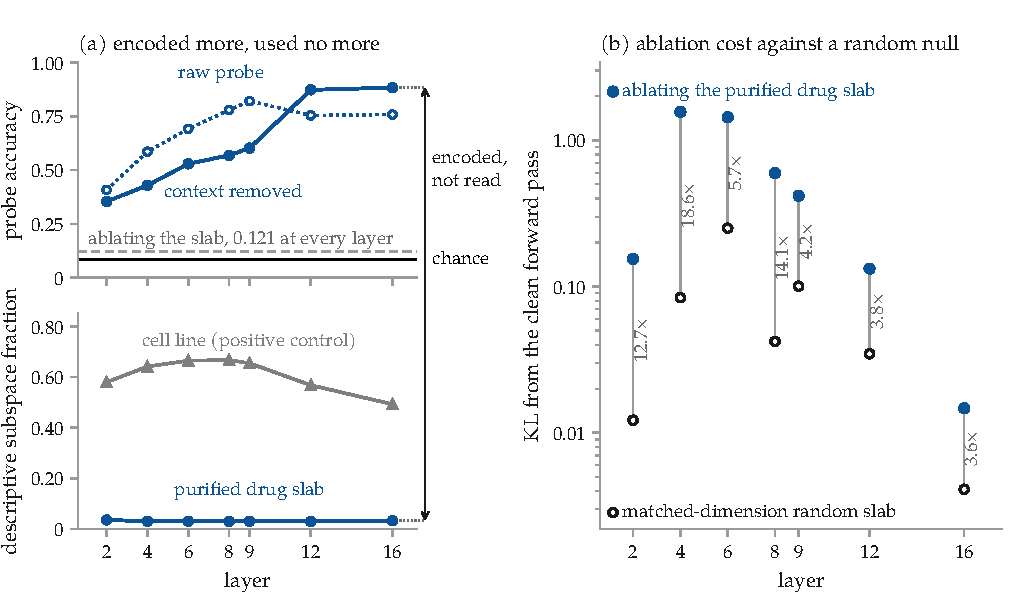
\includegraphics{fig-mechanism}
\caption[Decodable with depth, at a bit player's weight]{\textbf{Drug-label
information becomes more decodable with depth while interventions on the purified
slab have limited effect.} Layer is a true numeric axis in both panels, so the
9--12--16 spacing is drawn as it is.
(a) Top: drug-label probe accuracy over \emph{twelve} drug classes, so chance is
$1/12 = 0.083$; the raw probe is drawn for contrast and the flat grey line is the
same probe after the slab is projected out. Bottom: the descriptive subspace
fraction of the purified drug slab against the cell-line positive control, on its
own separate scale --- it is an activation-space summary, not a decomposition of
biological drug-response variance. The double-headed arrow at layer 16 spans the
two, and is what \emph{encoded, not read} names.
(b) Mean KL from the clean forward pass when the purified drug slab is ablated,
against a matched-dimension random subspace, $n = 60$ prompts per entry. Log
axis because late-layer divergences are small for everything, and paired dots
rather than bars: on a log axis a bar's length is measured from an arbitrary axis
floor, whereas the vertical gap between a pair \emph{is} their ratio, which is
the number annotated beside each pair and the number in
\cref{tab:workspace}. \textbf{No intervals are drawn in either panel.} The
stored dispersions are normal-approximation standard errors over the 60 prompts,
not the thesis's one interval convention (95\% bootstrap clustered over cell
lines); as in \cref{tab:workspace} this is a sign-and-magnitude reading and not
an estimate with an interval. These accuracies come from a different instrument
from the twenty-four-class probe sweep run over the five arms of
\cref{sec:res-mechanism}, whose chance is $1/24$ on a different label set, and
the two must not be read against each other. Whether drug \emph{identity}
is read requires \cref{sec:res-mechanism}.}
\label{fig:mechanism}
\end{fullwidth}
\end{figure}

\paragraph{Where ablation stops} It cannot show that the slab's drug-specific
content is what is read. The purified directions could carry generic
strong-programme energy that merely co-varies with drug across the twelve.
That needs a test which replaces what the slab says.

\begin{claim}
The purified drug-label slab carries decodable information and generation is
sensitive to its removal, at a bit player's weight. Once cell line, plate and
dose are projected out, decodability rises monotonically with depth, which the
raw probe, peaking at layer 9, does not, while the descriptive subspace fraction
stays flat at $\approx 0.03$, roughly $5\%$ of the cell line's $\approx 0.6$, and
is not a biological variance decomposition. Ablating the slab costs $9$--$37\%$
of what ablating cell line costs at layers $2$--$9$, with layer $12$ the
exception at $98\%$. Whether the slab's content is read, ablation cannot say.
\end{claim}

% ===========================================================================
\beatsection{E}{3}{Identity is read, at very low gain}{sec:res-mechanism}
% \claimlede must follow \beatsection: \beatsection clears the stored lede.
\claimlede{The generation decoder is sensitive to the drug-label activation
signal at very low gain, in one training arm and at one rung of the displacement
ladder.}

\begin{question}[3]
Removal cannot distinguish a region whose \emph{content} is read from one whose
mere presence matters. The last question needs an instrument that replaces what
the region says. Push the activations from the drug the prompt names towards
another drug, and ask whether the model moves its preference towards that other
drug's own held-out sentence. It moves, by a sliver, in one arm at one depth. The
design is given at length because three earlier versions could have manufactured
an effect.
\end{question}

\noindent
The verdict first, because the instrument takes several pages to describe and the
verdict is small. In one of the five training arms of \cref{tab:trainconfig}, at
one depth of seven, injecting half the class-mean displacement from drug A to
drug B inside
the purified subspace ($\alpha = 0.5$, the rung the multiplicity correction is
applied to) moves the model's preference towards drug B's own held-out sentence,
against an identically constructed injection naming a third drug, by
\ci{+0.0197}{+0.0063}{+0.0335} of the preference gap the model already has. One
to two per cent, against a $10\%$ margin pre-registered for calling an effect
material. Two further seeds reproduce it, and of twenty-six headline tests it is
the only survivor of multiplicity correction.

Read at face value that says the generation decoder does consult which drug the
region names, at a gain far too small to account for anything in
\cref{sec:res-blind}. Read with the multiplicity discipline below it says less.

\begin{scopelimit}[carried into \cref{sec:res-epsilon} and \cref{sec:limitations}]
This is the weakest load-bearing measurement in the chapter and it is carried as
such. No argument downstream rests on it alone, and a reader who discards it
entirely loses nothing that the drug-blindness result depends on. What the
following section tests is a prediction of the \emph{interpretation} of this
result, not the result itself, and the inference there is written to run one way
only for that reason.
\end{scopelimit}

\paragraph{First, a contrast score} It is
\begin{equation}
 \log P\!\left(g_B \mid \textrm{prompt}_A\right) \;-\;
 \log P\!\left(g_A \mid \textrm{prompt}_A\right),
\end{equation}
where $g_A$ and $g_B$ are real cell sentences emitted under drugs A and B by
held-out cells, each log-probability a per-token mean. Any offset uniform across
positions, an inflated logsumexp normaliser included, then cancels exactly. It
does \emph{not} cancel in the stronger sense one might assume. Once $g_A$ and
$g_B$ diverge the two teacher-forced sequences visit different states, so the
normaliser's state-dependent part survives, unbounded here. The \texttt{permuted}
arm controls for that, sharing anchor, construction and norm and differing only
in naming the wrong drug. What survives the two-arm comparison is the model's
preference between drug B's own held-out sentence and drug A's.

\paragraph{Second, one anchor and one norm} Writing $\Pi$ for the orthogonal
projector onto the purified slab, the \texttt{swap} arm injects
$\Pi(\mu_B - \mu_A)$, pointing at the drug whose sentence is scored; the
\texttt{permuted} arm injects $\Pi(\mu_C - \mu_A)$ at identical norm, same anchor
and construction, wrong drug. An isotropic random direction is kept only as a
damage diagnostic, since it can disrupt the model in ways an observed class-mean
displacement does not. The subtraction cancels the global mean exactly, and
nothing is ablated, so the control has no removed term to trip over.

\paragraph{The three failed designs taught the constraints} A control drawn in
the full $2048$-dimensional stream puts $\approx 99.5\%$ of its energy where the
intervention never acts, so it must live in the treatment's subspace.
Ablate-then-add delivers (added $-$ removed), so an uncentred class mean turns
substitution into restoration, hence no ablation and an exactly centred
displacement. A norm-matched random direction inflates the logsumexp normaliser
(measured $+2.75$ nats), depressing every target whether or not it carries
identity. The planted-world selftest validates the directional logic but cannot
speak to the normaliser, since there each drug's sentence is a single token.
Algebra in \cref{sec:app-identity}.

\paragraph{Out of sample, and on a comparable scale} Subspaces and class means are
fit on one slice of cells; $g_B$ comes from a third disjoint slice, never from
the rows defining $\mu_B$, else the injected vector and the scored sentence would
share cells and the test would be partly circular. Because the five arms emit
different target formats, every effect is divided by that model's own clean
preference gap, measured with no intervention.

\paragraph{Four guards carry the inference} A drug-proxy screen and an
injected-norm diagnostic are engineering, deferred to \cref{sec:app-identity}.

The first is the uncertainty model, a cluster bootstrap over ordered (A,B) pairs,
because rows sharing a pair share the injected vector and the scored sentence. At
the anchor seed's layer $12$ that is $60$ rows in $58$ pair clusters over $24$
anchor drugs, close to a row bootstrap. It guards against sharing within a pair,
not across pairs sharing an anchor or target drug.\gloss{cluster
bootstrap}{resamples whole (A,B) pairs, not rows, so a shared vector
counts once}

The second is the equivalence criterion, stricter than TOST. The interval must
lie inside a pre-registered margin, set at $10\%$ of the model's own clean
preference gap, \emph{and} contain zero. That conjunct runs one way only; it can
withhold an equivalence verdict, never manufacture one. Under textbook TOST the
headline \ci{+0.0197}{+0.0063}{+0.0335} lies wholly inside the margin and would
be returned as equivalent, read as a null; this rule returns a directional effect
smaller than the margin.

The third is a per-layer headroom gate, excluding any layer where the cell-line
positive control shows less than $5\times$ dynamic range, because a saturated
instrument can support neither verdict. The fourth is a magnitude ladder,
repeating the test at $\alpha \in \{0.5, 1, 2, 5, 10\}$ times the natural
displacement, because a real identity effect should show a monotone
dose--response. The ladder is the guard that bites.

\paragraph{One survivor in twenty-six tests} The design ran across the five
training arms of \cref{tab:trainconfig} and, for the two residual arms, at three
further seeds. Of $26$ headline tests, five arms by up to seven depths, exactly
one survives Benjamini--Hochberg correction, the residual arm at layer $12$
($q = 0.026$, pooling the $26$ across arms and not correcting within each as the
pipeline stores them). That $q$ rests on a bootstrap $p$, and the arm's probe
file carries two draws of it for the same effect, identical to sixteen digits, at
$p = 0.001$ and $p = 0.004$, either side of the $0.05/26$ admitted at rank one;
on the second draw nothing survives. The consensus arm at layer $2$ ($p = 0.012$)
does not ($q = 0.156$).

\paragraph{Which rung the correction is applied to matters} The headline is the
$\alpha = 0.5$ rung, half the natural displacement, so the ladder's first entry
is that headline in raw nats ($+0.0013$) and not an independent point. At full
displacement the effect is \emph{larger} and noisier,
\ci{+0.0265}{+0.0021}{+0.0524} against \ci{+0.0197}{+0.0063}{+0.0335}, at
$p = 0.033$ against $p = 0.001$ on the draw the correction uses. Each of
$\alpha = 0.5$, $1$ and $2$ excludes zero; $\alpha = 5$ and $10$ span it. In raw
nats the rungs read $+0.0013$, $+0.0017$, $+0.0044$, $+0.0061$, $+0.0046$, rising
to $\alpha = 5$ and turning over at $\alpha = 10$ (\cref{fig:family}, lower
strip), consistent with a dose--response without establishing one. All five
re-score the same $60$ rows at scaled injection, no trend statistic is computed,
and the pre-registered monotonicity holds over four rungs of five.

But applying the $26$-test correction to the $\alpha = 1$ slice leaves
\emph{nothing} surviving, and applying it to $\alpha = 2$ promotes a different
arm at a different depth (\texttt{residual\_holdout} at layer $4$, $q = 0.007$)
while demoting this one (\cref{fig:family}). The slice decides not merely
whether a survivor exists but which one, and below that the bootstrap draw
decides whether one exists at all. That is the mark of a family dominated by
noise, not of one containing a single robust effect. The multiplicity-corrected
claim is therefore a statement about the $\alpha = 0.5$ slice and is not robust
to that choice, which is why this section opened by discounting its own result
instead of closing on it.

% ===========================================================================
\begin{figure}[htbp]
\begin{fullwidth}
\centering
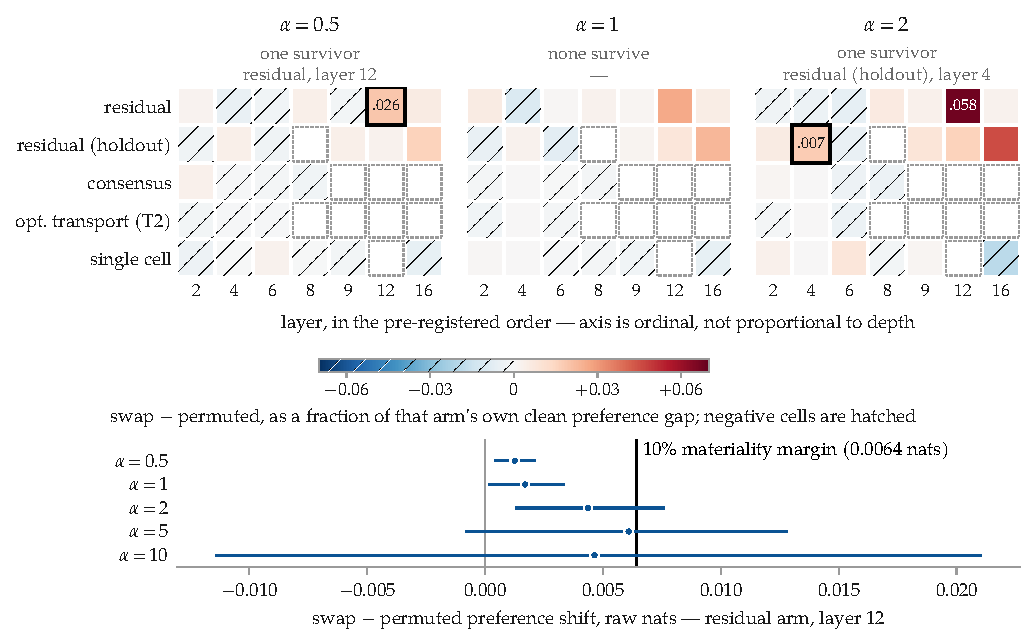
\includegraphics{family}
\caption[The single survivor moves with the rung]{\textbf{The one test that
survives multiplicity correction changes arm and depth with the rung of the
displacement ladder, and at one rung there is no survivor at all.} Each panel is
one slice of the ladder: the five training arms of \cref{tab:trainconfig} (rows)
by the seven probed depths (columns), $n = 26$ measured tests per slice, on one
diverging scale shared across the three panels. Colour is the \texttt{swap}
minus \texttt{permuted} effect as a fraction of that arm's own clean preference
gap. The layer axis is ordinal, drawn at equal spacing, and is not proportional
to depth. Nine of the $35$ grid positions were never measured and are drawn as
empty dotted outlines, not as zeros. Benjamini--Hochberg is pooled across arms
within a slice, as the text applies it and not as the pipeline stores it; $q$ is
printed in the three cells that fall below $0.10$ and ringed where $q < 0.05$.
That criterion admits the residual arm at layer $12$ at $\alpha = 0.5$
($q = 0.026$, on the stored bootstrap draw the text discusses), nothing at
$\alpha = 1$, and \texttt{residual\_holdout} at layer $4$ at $\alpha = 2$, which
demotes layer $12$ to $q = 0.058$; it is the only survivor among this chapter's
twenty-six headline tests. Beneath, the same residual arm at layer $12$ in raw
nats across all five rungs, with the $10\%$ pre-registered materiality margin as
the vertical rule. Intervals throughout are $95\%$ cluster bootstraps over
ordered (A,B) pairs, $4000$ resamples, which at this layer is $60$ rows in $58$
pair clusters over $24$ anchor drugs. The three seed replicates are in
\cref{tab:identity} and are deliberately not drawn here.}
\label{fig:family}
\end{fullwidth}
\end{figure}

% ===========================================================================
\begin{table}[htbp]
\begin{fullwidth}
\begin{threeparttable}
\caption{\textbf{The identity test replicates in the arm that behaviour calls
drug-sensitive and is absent in the arm behaviour calls drug-blind.} Effects are
a fraction of that model's own clean preference gap between the two sentences
compared (mean effect $+0.0133$ across the three seeds that measured it). The $p$
column is a two-sided cluster bootstrap over $4000$ resamples floored at
$1/4000$; seed 43's entry is that floor, reached when no resample fell at or
below zero, so it is a resolution limit and not a measurement. Seed 44 produced
no layer-12 measurement, and five of its seven layers were skipped because the
purified slab retained context, not for want of headroom; those five carry
headroom of $9.7$ to $23.3$. The pre-registered criterion of two replications in
three new seeds is met, the third a non-measurement and not a failure.}
\label{tab:identity}
\small
\begin{tabular}{@{}lrrr@{}}
\toprule
\thead{Arm / seed} & \thead{effect} & \thead{95\% CI} & \thead{$p$} \\
\midrule
residual, seed 42 & $+0.0197$ & $[+0.0063, +0.0335]$ & $0.0010$ \\
residual, seed 43 & $+0.0118$ & $[+0.0060, +0.0173]$ & $0.00025$ \\
residual, seed 45 & $+0.0085$ & $[+0.0029, +0.0143]$ & $0.0015$ \\
\midrule
single-cell arm, six depths
  & \multicolumn{3}{l}{nothing detectable at any depth (median $-0.0012$)} \\
\bottomrule
\end{tabular}
\begin{tablenotes}[flushleft]\footnotesize
\item The rows are the headline $\alpha = 0.5$ rung, to which the multiplicity
correction that admits the first row is applied and to no other.
\end{tablenotes}
\end{threeparttable}
\end{fullwidth}
\end{table}

% ===========================================================================
\paragraph{The instrument has been shown to register a positive} The residual arm
is independently known to respond to the drug its prompt names. On \texttt{train},
swapping the named drug and its mechanism for an orthogonal partner costs it
$+0.0898$ in $\NIR$, excluding zero clustered on cell line
($[+0.0382, +0.1415]$) and on drug ($[+0.0291, +0.1506]$), a behavioural result
established in \cref{sec:res-generalisation}. \forward{sec:res-generalisation}

Three things bound what it licenses. It is a training-split fact, and does not
extend to held-out combinations. It is behavioural, so it says the arm responds
to the drug its prompt names, not that the response is routed through the
subspace this test injects into. And the two measurements are not on the same
weights, the swap gap scored on the rebuilt target build and this probe on the
earlier one (\cref{tab:trainconfig}), so drug-sensitivity and identity reading
are attributed to residual-target training and not to any checkpoint. Narrower
than a routing claim, and enough. The probe detects identity reading, replicably,
in the arm behaviour calls drug-sensitive, and none at any depth in the arm that
is behaviourally drug-blind. A null from an instrument never shown to register a
positive is uninterpretable; this one has.

\paragraph{Three limits belong with the verdict} The effect appears at one depth
of seven, and layer 4 is positive in a single seed and null in the other three.
The single-cell arm has no layer-12 measurement, its cell-line positive control
reaching $3.88\times$ there, under the $5\times$ gate; so the cleanest
comparison, the same depth across two arms, does not exist, and the dissociation
rests on that arm being null at all six depths it could measure. And the sibling
residual-holdout arm does not reproduce the effect at the headline rung
($+0.0028$ and $+0.0049$ in the two seeds where it was measured); it surfaces
instead at $\alpha = 2$, rung-dependence and not a second replication.

Read with the decodability series, the picture is label information that becomes
more linearly decodable with depth once cell line, plate and dose are projected
out, while the process that writes the prediction barely consults it. That is
suggestive of the workspace account of \cref{sec:lit-interp}, an interpretation
of the pattern and not a demonstration of the mechanism.

\begin{claim}
The anchor seed puts it at \ci{+0.0197}{+0.0063}{+0.0335} of the model's own
preference gap, and $+0.0133$ averaged over the three seeds that measured it, one
to two per cent, a fifth or less of the $10\%$ margin pre-registered for calling
an effect material. The multiplicity-corrected version of that holds for the
$\alpha = 0.5$ rung on one of its two stored bootstrap draws, not for its
neighbours. At $\alpha = 1$ nothing survives correction; at $\alpha = 2$ a
different arm does. The claim is not that the decoder cannot read drug identity,
and it is not the stronger mechanistic story earlier drafts told.
\end{claim}

% ===========================================================================
\beatsection{E}{4}{Denoising the target changes the target, not the decoder}{sec:res-epsilon}

\begin{question}[4]
If the defect is a decoder that barely consults the drug region whatever is
written there, then improving what sits in that region should not help, and
improving the training target is exactly that kind of intervention. It is also
the repair a reader reaches for first, which is reason enough to test it. Three
target constructions, one scoring, one stratum. None separates from a prompt
naming the wrong drug.
\end{question}

\noindent
The interpretation at the end of the last section is \notestablished, and this
section does not proceed as though it were. The inference runs one way only. A
positive here would tell against the low-gain reading; a negative is evidence
about target-side fixes, not confirmation of the mechanism. Because one failed
construction proves nothing, two more were compared with it.

\paragraph{Three points, not a sweep} They are the original single-cell target,
one optimal-transport barycentre and the consensus target. \emph{Consensus}
groups cells by (drug, cell line, dose) and averages them into one pseudobulk
sentence, every original prompt retained so only the target changes.
\emph{Optimal transport} uses the full condition key carried by the source,
(cell line, plate, drug, dose/treatment well), computing each condition
separately, its treated cells coupled only to the shared DMSO controls from that
condition's own (cell line, plate). Treatment conditions are never pooled.

The coupling $\pi$ minimises $\sum_{ij}\pi_{ij}\lVert x_i - y_j\rVert^2$ under
balanced uniform marginals, which impose mass conservation between the empirical
control and treated measures, a modelling assumption and not an observed
biological constraint. Sinkhorn iteration~\cite{cuturi} solves it on the kernel
$\Gamma = \exp(-C/\varepsilon)$, with $C$ the pairwise squared-distance matrix.
Couplings are computed in the released Tahoe scVI latent~\cite{scvi}
($n_{\textrm{latent}} = 10$), joined per cell by barcode and not re-encoded,
since a re-encode produced a degraded latent (cell-line probe $0.11$ versus
$0.975$). Targets are built without the scVI decoder, as convex combinations of that
condition's observed treated cells, so they stay inside their convex hull, not
necessarily on the data manifold.

The regularisation parameter locates the middle construction between two limits.
As $\varepsilon\rightarrow\infty$ the coupling is uniform and the target is the
treated mean (consensus); as $\varepsilon\rightarrow 0$ it approaches an
unregularised sparse transport solution, not necessarily a map to one observed
treated cell. Only three hand-picked constructions were trained and scored, so
this is a three-point comparison and not a sweep of the family.

\paragraph{One scoring, named before the result} Every point was scored on the
identifiable stratum, the conditions \cref{sec:res-blind} selected because their
own within-well reference clears the pre-set $0.80$ bar, under the random-partner
scramble defined there. That is the stratum on which a zero-drug-information
control-copy already matches the model, so the scope limit of
\cref{sec:methods-probe} applies to every row of \cref{tab:epsilon}.

% ===========================================================================
\begin{table}[htbp]
\begin{fullwidth}
\begin{threeparttable}
\caption{\textbf{Three target constructions, and no point separates from its
random-partner scramble on the identifiable stratum} ($n = \num{204}$). Two
things bound that negative. The consensus endpoint was stopped at roughly $60\%$
of an epoch with its tier-1 NIR unscoreable, so the negative rests on the
single-cell and optimal-transport endpoints. And the optimal-transport endpoint
is not null in every frame. These rows use a random partner at $1200$ generation
tokens, while against the geometry-defined \texttt{orth} partner over all its
conditions the same checkpoint moves from \ci{+0.0144}{-0.0051}{+0.0338} at $600$
($n = \num{250}$) to \ci{+0.0292}{+0.0144}{+0.0441} at $1400$ ($n = \num{248}$),
reported in \cref{sec:res-encoding}. Comparator, population and budget differ at
once, and \cref{sec:methods-data} shows the budget is a claim-level variable, so
the frames are set side by side and not put into ratio. This is a null under this
scoring, not over the family of target constructions.}
\label{tab:epsilon}
\small
\begin{tabular}{@{}llll@{}}
\toprule
\thead{Target} & \thead{$\varepsilon$} & \thead{$\gap$} & \thead{Verdict} \\
\midrule
single cell (real treated cell) & $\approx 0$
  & \ci{+0.014}{-0.016}{+0.042} & not separated \\
OT barycentric & $0.5$
  & \ci{-0.001}{-0.018}{+0.016} & not separated \\
consensus (global mean) & $\rightarrow\infty$
  & \ci{-0.010}{-0.022}{+0.003} & not separated \\
\bottomrule
\end{tabular}
\begin{tablenotes}[flushleft]\footnotesize
\item $\gap$ is the model's $\NIR$ minus its scramble's, so its null is zero and
not chance. The three rows share a scoring, a stratum and a comparator; they are
one comparison, not three independent experiments. All three intervals are
\emph{one-way} percentile cluster bootstraps over the $40$ cell lines, not the
two-way default.
\end{tablenotes}
\end{threeparttable}
\end{fullwidth}
\end{table}

% ===========================================================================
An interval that covers zero earns its keep by what it excludes. On the
identifiable stratum the single-cell arm's scramble gap is
\ci{+0.014}{-0.016}{+0.042}, against the $0.170$ separating the model's $0.768$
from that stratum's $0.938$ reference. At the very top of the interval, naming
the right drug instead of a wrong one would buy a quarter of what is there to be
bought, and the point estimate puts it at $8\%$ of that. Taking that distance at
face value is the generous reading, for the reason declared in
\cref{sec:methods-probe}. The interval does not show the effect is zero and no
experiment here could; it puts it far below the room these conditions leave.

% ===========================================================================
\paragraph{Training was not inert, and what it did instead is a result} The
consensus model stops echoing the control. On the identifiable stratum it scores
$0.653$ against a zero-drug-information control-copy at $0.766$, where the
single-cell model sits on the control at $0.768$. Its predictions are not
mode-collapsed either; there is real between-condition variation. But that
variation is uncorrelated with real drug identity. The Mantel correlation between
the model's between-drug distance structure and the true one averages $+0.03$
over cell-line and plate groups.

The failure this literature names first for a perturbation model that
underperforms on well-calibrated metrics is mode collapse, where the prediction
ignores the input and reverts to a mean, and the repair is to restore diversity
in what the model emits~\cite{mejia}. This arm is not that. It moved off the control, kept the
variation, and spent it on the wrong axis. Producing no structure and producing
structure that does not track the drug are different failures with different
repairs.

\begin{claim}
No point in the three-point comparison separates from its scramble on the
identifiable stratum under the random-partner test. Two things bound that
negative. The consensus arm was stopped mid-epoch, so the comparison rests on the
single-cell and optimal-transport points, and the optimal-transport arm is not
null in every frame: scored against the geometry-defined \texttt{orth} partner
over all its conditions at the residual arm's generation budget, its gap excludes
zero (\cref{sec:res-encoding}). By the inference rule above that positive tells
against the low-gain reading and not for it, and being in a different frame
it does not settle the matter, but it is one more reason the interpretation of
\cref{sec:res-mechanism} is carried here as an interpretation and not a result.
What the comparison establishes is that denoising the target changes what is in
the target without changing what the decoder does with it under this scoring, and
not that no target-side fix can work. Measuring how much of the target its tokens
expose to the drug, which the next two sections do, is not the same as showing
that the target encoding is the defect (\cref{sec:methods-residual}). That
construction changes five things at once.
\end{claim}

% ...........................................................................
% 04c-reencoding.tex -- beats 5-6. The residual re-encoding.
% Legacy anchors sec:methods-vardecomp and sec:methods-holdout are re-\label-ed
% here so v1 cross-references resolve.
% ...........................................................................

\beatsection{R}{5}{The standard target hides the drug}{sec:methods-residual}

\begin{question}[5]
A sentence lists genes in order of expression, so two drugs on the same
cells give almost the same target string and the loss can barely tell them apart.
Can the target be rewritten so that its tokens \emph{are} the drug-specific part?
The instrument counts how many top target positions carry a different gene for
two drugs in one context. Almost none do before the rewrite; a clear majority do
after, at an unchanged retrieval reference.
\end{question}

\noindent
\emph{Encoding} here means how the target string is written, not what the model's
internal states carry (\cref{sec:res-used}). The loss weights every position
equally, so the measurement is a count over the $200$ target positions
(\cref{tab:divergence}).

% ...........................................................................
\begin{table}[htbp]
\begin{threeparttable}
\caption{\textbf{$83\%$ of the standard target's tokens are identical between
any two drugs in the same context.} The residual row is quoted at cell-line
scope; at plate scope it reads $120.3$ and $0.7467$. The middle column is where
the three encodings differ, and it does not on its own identify tokenisation as
the binding constraint.}
\label{tab:divergence}
\small
\begin{tabularx}{\linewidth}{@{}%
  >{\raggedright\arraybackslash}p{0.34\linewidth}
  >{\raggedright\arraybackslash}p{0.28\linewidth}
  >{\raggedright\arraybackslash}X@{}}
\toprule
\thead{Representation} & \thead{Top-$200$ tokens differing between drugs}
  & \thead{Within-well split-half retrieval reference} \\
\midrule
full profile (the standard target) & $34.6$ / $200$ \;($17\%$) & $0.742$ \\
shift (treated $-$ control)        & $111.4$ \;($56\%$)        & $0.742$ \\
\textbf{residual (drug-specific)}  & $118.2$ / $200$ \;($59\%$) & $0.7432$ \\
\bottomrule
\end{tabularx}
\begin{tablenotes}[flushleft]\footnotesize
\item The two columns hold different quantities, a count out of $200$ positions
and a retrieval score, so rows compare within a column and never columns with
each other. The third column pits disjoint cell subsets of one drug, in one cell
line, on one plate, against each other. It is a precision reference, not a
biological replicate ceiling, and it is near-constant across the three rows.
\end{tablenotes}
\end{threeparttable}
\end{table}

\paragraph{The count stops short of the tokenisation claim} The natural
inference, that only a small fraction of the gradient carries drug identity, is
a hypothesis about the optimisation; what is measured is the overlap of target
gene sets, not a token-level loss or a gradient attribution. Gene positions are
not loss-token positions under byte-pair encoding, and the residual target below
alters aggregation, control referencing, generic subtraction, sign coding and
sequence length at once. Separating those five factors needs a matched-budget
factorial this thesis does not run.

\paragraph{The count is not inherited from residual similarity} A descriptive
summary bins $212{,}528$ exhaustive within-group drug pairs on the cosine between
the two residuals. Mean differing top-$200$ genes across the near,
orthogonal and opposite strata run $32.5$, $34.6$ and $35.8$ for the full
profile; $107.4$, $111.3$ and $114.4$ for the shift; $118.4$, $121.0$ and
$118.7$ for the residual, with Spearman coefficients against residual cosine of
$-0.149$, $-0.282$ and $+0.019$. The residual target stays high in every stratum
and lacks the monotone gradient the other two carry, which weakens the reading
that the later swap-distance pattern is inherited trivially from target
divergence without being an independent test of it. The pairs reuse drugs and
groups, so no pair-level inferential claim is made.

% ...........................................................................
\begin{defn}{The drug-specific residual}
For each condition, a (drug, cell line, plate, dose) tuple with at least $40$
treated and $20$ plate-matched control cells,
\begin{equation}
 \resid(d,c) \;=\; \underbrace{\big(\bar{y}_{\textrm{treated}} - \bar{y}_{\textrm{control}}\big)}_{\shift(d,c)}
 \;-\; \underbrace{\frac{1}{|D_c \setminus \{d\}|}\sum_{d' \in D_c,\; d' \neq d} \shift(d',c)}_{\textrm{generic}(c)} .
\end{equation}
The control subtraction removes the cell's own state, leaving the \emph{shift};
the mean over drugs removes the \emph{generic} drug programme every drug
triggers. $D_c$ is the training drugs sharing $c$'s plate and cell line, each
entering once whatever its doses, and the condition's own drug is excluded.
What remains is not what makes this drug different from all drugs. It
is what makes it different \emph{from the other training drugs that happen to
share its plate and cell line}.
\end{defn}

\paragraph{The comparison set is fixed by the plating design} That last sentence
is the price of estimating the generic locally, and mechanism is where it bites.
\Cref{sec:res-scope} finds mechanism-related drugs co-plated $0.404$ of the time
against $0.362$ for a random draw, so for a co-plated mechanism class part of the
class's own shared programme sits inside the generic and is subtracted out of
every member's residual by construction.

That bias was tested. Same-mechanism plate-mates supply a mean $4.4\%$ of a
condition's generic, present for $83\%$ of the $\num{917}$ labelled
mechanism-arm conditions, from Tahoe's \texttt{moa-fine} labels joined to the
plate rosters the channel gate scored. The $\num{155}$ conditions with \emph{no}
same-mechanism plate-mate, whose residuals retain the mechanism programme, give a
gap of \ci{+0.1145}{+0.0276}{+0.2014} against \ci{+0.0737}{+0.0150}{+0.1324} for
the $\num{762}$ that have one, both against the same plate-matched null under the
same two-way clustering. That is the direction the construction predicts, but not
a corrected estimate. The intervals overlap across almost their whole range, the
split is post hoc, and the cleaner stratum rests on $\num{43}$ wells. It supports
a statement about sign, not size.

\begin{scopelimit}[carried into \cref{sec:res-scope} and \cref{sec:limitations}]
Two properties of this frame travel with every number measured in it. First, the
generic is a plate-local mean, so where a mechanism class is co-plated the
mechanism channel is later graded in a frame that has already removed some of
what it is asked to find, which makes an inconclusive verdict on mechanism the
conservative reading and not a generous one. Second, the plate-scoped generic
removes plate structure from the truths and, in expectation, from the
predictions, but that is an expectation and not an identity. An individual
residual may retain some plate structure, and the size of what remains was never
measured. The absolute $\NIR$ values of this frame are read within it and never
set beside the within-plate tables elsewhere in the chapter.
\end{scopelimit}

\paragraph{Which subtraction does the work} Removing the control moves the
between-drug token difference from $34.6$ to $111.4$; removing the generic adds a
further $6.8$ at cell-line scope and $8.9$ at the plate scope this build uses. So
the control subtraction alone buys $92\%$ of the recoverable difference, $90\%$
plate-scoped. The measurement is an overlap of gene sets on one atlas at $K = 200$
($\num{6602}$ conditions, \texttt{target\_divergence.json}), so no margin is
claimed for other atlases or other $K$. It squares with \cref{sec:res-metrics},
where what saturates $\DEdr$ is reversion toward a central point,
\texttt{revert\_center} scoring $0.9999$ without fitting anything.

The generic is not dispensable. It carries $39\%$ of the shift's energy
(\cref{sec:res-transfer}), and subtracting it isolates the drug-specific
remainder once the baseline is gone. The inclusion thresholds sit where the
identifiability curve of \cref{sec:res-blind} flattens, the within-well
split-half precision reference being $0.61$ at $10$ cells, $0.76$ at $40$ and
$0.85$ at $120$.

% ...........................................................................
\paragraph{A definition that could have been circular, and what breaks it} Four
properties of how the generic is estimated decide whether the remainder can be
trusted. First, the shape of the problem. A condition enters training only if its
residual reproduces across a half-split; a residual exists only once the generic
has been subtracted; the generic is fitted on the training set; and the training
set is what the reliability line selects. That is a loop
(\cref{fig:circularity}, left), and an earlier build closed it, with generic and
filter estimated over every condition and the holdout assigned afterwards, so
each held-out target was defined partly by other held-out conditions.

The loop is cut by ordering. Inventory and split read metadata only, before any
pseudobulk exists; fit hands the generic the training keys explicitly; transform
projects held-out conditions through the fitted generic, which they never enter
(\cref{fig:circularity}, right). Because the split is made on metadata alone,
nothing downstream of it can have defined it. A poison test makes the ordering
checkable in both directions.\gloss{poison test}{Corrupt the held-out side; the
training targets must not move. Corrupt a training condition; they must.} The
other three properties fix choices the staging leaves open.

% ===========================================================================
% circularity.tex -- the residual definition's loop, and the ordering that cuts
% it. \input by Sections/04c-reencoding.tex at sec:methods-residual. Compiles
% against thesis_v2/preamble.tex and nothing else: no external data, no
% \includegraphics, no package this document does not already load
% (tikz + arrows.meta, both in preamble.tex section 9).
%
% THIS IS A PROVENANCE DIAGRAM, NOT A RESULT. Deliberately absent: every NIR
% value, every arm, every split-level number. Two counts appear, once, and both
% are already in the prose of this same section. Sibling circularity.json lists
% every number drawn.
%
% THE LEFT PANEL CARRIES NO BUILD LABEL, DELIBERATELY. It drew "THE EARLIER
% BUILD -- NOT THE SHIPPED ONE" until this revision, which spent half a
% full-width figure on a pipeline the thesis did not run. The historical fact
% -- that an earlier build did close this loop -- is a disclosure, and a
% disclosure belongs in prose where it can be qualified: it is stated at
% Sections/04c-reencoding.tex:148-151 ("That is a loop [...], and an earlier
% build closed it, with generic and filter estimated over every condition and
% the holdout assigned afterwards"). That sentence stands on its own and was
% NOT deleted when the label came off the panel. What the left panel draws now
% is the structural hazard itself, in the present tense and attached to no
% build: the cycle the four definitions form, and the edge that fitting before
% splitting adds to it. The two panels therefore read hazard and remedy, which
% is the only reason the staged ordering is load-bearing rather than fastidious.
%
%   2,523 of 4,999 training conditions retained (50.5%)   04c-reencoding.tex:211-212
%   the resolved reliability line, +0.1086                 04c-reencoding.tex:211
%
% Cross-checked, all four agreeing, before drawing:
%   Sections/03-Apparatus.tex:206     "2,523 of 4,999 train (50.5\%)"
%   Sections/04c-reencoding.tex:212   "$2{,}523$ of $\num{4999}$ ... ($50.5\%$)"
%   Sections/04d-baselines.tex:337    "only $\num{2523}$ are training"
%   Sections/05-Limitations.tex:33    "$\num{2523}$ of $\num{4999}$ ... $\cos > 0.109$"
% +0.109 is the measured null's 95th percentile and +0.1086 is what it resolves
% to; the prose prints both, and the node carries the resolved value because
% that is the one the builder applies.
%
% LAYOUT NOTES, all forced by a build:
%   * fullwidth = 174mm = 493.23pt (textwidth 142mm + marginparsep 4mm +
%     marginparwidth 28mm, preamble.tex:88-90 and :525). The bounding box is
%     PINNED to 17.35cm = 491.81pt, 1.4pt inside the measure. Unpinned, the
%     picture measured 3.10pt OVER and the figure body reported an overfull
%     hbox: nodes with anchor=north west hang their 3.33pt inner sep left of
%     the anchor at x=0.20, and the strip rules end at x=17.35. Pinning clips
%     no ink -- no drawn object lies outside [0, 17.35] x [-0.95, 7.95].
%   * NO node uses text width. Every line break is written by hand. The first
%     build did use text width and TeX hyphenated inside the boxes
%     ("the relia-/bility line"), grew four of them past their minimum heights
%     and overlapped the rows below. Hand-broken lines make every box width and
%     height deterministic, which is what lets the coordinates below be trusted.
%   * the four objects are ONE node set drawn twice, same style, same wording,
%     same 2.80cm minimum width, so the right panel reads as a re-laying of the
%     left and not as a second diagram. Only the arrangement changes.
%   * the fatal edge is drawn and STRUCK, not deleted. A deleted edge leaves
%     nothing for the caption to point at, and the passage is about which single
%     edge the ordering removes.
%   * the two streams leaving SPLIT must not cross. They cannot both turn upward
%     in the order they leave: the stream that leaves HIGHER (held-out, 2.2mm
%     above the east anchor) turns up FIRST (x=10.30) and the stream that leaves
%     LOWER (training keys, at the east anchor) turns up LATER (x=10.85). Any
%     other pairing crosses, and a crossing here reads as contact between them.
%   * both streams use -| rather than an explicit corner coordinate, so the
%     corner inherits the node anchor's own y. Written as a literal corner, the
%     first segment came out as a visible diagonal whenever a node's height
%     differed by a hair from the value assumed at design time.
%   * the held-out stream is routed over the top of the fit column, and its one
%     arrowhead points right, into TRANSFORM. No arrowhead anywhere in the right
%     panel points back left or up into the fit; that absence is the claim.
%   * NO edge label is masked onto its arrow. The first build masked all of
%     them and the labels ate the edges: the C->D gap in the left panel is
%     1.20cm and "subtracted to give" is 1.15cm wide, so the bottom edge of the
%     cycle disappeared and the loop stopped reading as a loop. Every label now
%     sits beside its edge. The tightest is "training keys", hung under the
%     corner at x = 10.43 to 11.27, between the held-out riser at 10.30 and the
%     fit column's left edge at 11.35.
% ===========================================================================
\begin{figure}[htbp]
\begin{fullwidth}
\centering
\begin{tikzpicture}[x=1cm, y=1cm]
  \useasboundingbox (0,-0.95) rectangle (17.35,7.95);
  \tikzset{
    % the shared node set. Identical style in both panels.
    obj/.style={draw=rulegrey, line width=0.4pt, fill=white, inner sep=3pt,
                align=center, font=\scriptsize, text=ink,
                minimum width=2.80cm, minimum height=0.68cm},
    edg/.style={-{Stealth[length=3.6pt,width=2.8pt]}, draw=ink,
                line width=0.5pt},
    lab/.style={font=\scriptsize, text=quietink, fill=white, inner sep=1pt,
                align=center},
    side/.style={font=\scriptsize, text=quietink, align=flush right,
                 anchor=east, text width=3.20cm},
    quiet/.style={font=\scriptsize\itshape, text=quietink, align=center},
    tag/.style={font=\sffamily\scriptsize\bfseries, text=accent},
    sub/.style={font=\footnotesize\itshape, text=quietink}}
  \def\T#1{{\sffamily\scriptsize\bfseries\color{accent}#1}\\[1.0pt]}
  \def\Q#1{\\[1.0pt]{\color{quietink}#1}}

  % ======================= PANEL HEADS =====================================
  % Hazard and remedy, one head each, same shape: a tag naming the structure
  % and a sub saying what happens to the four objects. Neither names a build.
  \node[tag, anchor=north west] at (0.20,7.90) {THE CIRCULARITY};
  \node[sub, anchor=north west] at (0.20,7.55)
    {the four objects define one another};
  \node[tag, anchor=north west] at (7.50,7.90) {THE ORDERING THAT CUTS IT};
  \node[sub, anchor=north west] at (7.50,7.55)
    {the same four objects, staged by execution order};

  \draw[rulegrey, line width=0.4pt] (7.20,1.15) -- (7.20,6.60);

  % ======================= LEFT: THE CLOSED LOOP ===========================
  \node[obj, anchor=north] (A) at (1.60,6.10) {the reliability line};
  \node[obj, anchor=north] (B) at (5.60,6.10) {the training set};
  \node[obj, anchor=north] (C) at (5.60,4.45) {the generic};
  \node[obj, anchor=north] (D) at (1.60,4.45) {the residual};

  % NONE of the four loop labels is masked onto its arrow. Masked, they ate the
  % edges: the C->D gap is 1.20cm and "subtracted to give" is 1.15cm wide, so
  % the bottom edge of the cycle vanished entirely and the loop stopped reading
  % as a loop. Each label now sits beside its own edge -- the two horizontals
  % labelled outside the cycle, the two verticals inside it -- and all four
  % edges draw unbroken.
  \draw[edg] (A.east) -- (B.west);
  \draw[edg] (B.south) -- (C.north);
  \draw[edg] (C.west) -- (D.east);
  \draw[edg] (D.north) -- (A.south);
  \node[lab, anchor=south] at (3.60,5.86) {selects};
  \node[lab, anchor=east]  at (5.45,4.94) {fits};
  % clears the box row's bottom edge at y=3.77: at y=3.97 its first line sat
  % level with the two boxes' lower corners, 0.02cm from each, and read as a
  % collision even though it was not one.
  \node[lab, anchor=north] at (3.60,3.88) {subtracted\\to give};
  \node[lab, anchor=west]  at (1.75,4.94) {must reproduce\\across a half-split};

  % --- the fatal edge: drawn once, struck once, and labelled --------------
  % Present tense, and attached to an ordering rather than to a build: this is
  % what fitting before splitting does to the cycle, not what one run once did.
  % The quiet italic under H answers "why would they enter the fit?" inside the
  % panel, and mirrors the right panel's one quiet italic under SPLIT, so each
  % half carries exactly one such annotation.
  \node[obj, anchor=north] (H) at (1.60,2.60) {held-out conditions};
  \draw[edg] (H.east) -| (C.south);
  \node[lab, anchor=east] at (5.45,2.95) {enter the fit};
  % Its y is the strike caption's y, not a value of its own: both are two-line
  % blocks of the same size, so sharing anchor y = 1.74 gives them a common top
  % AND a common bottom (0.944) and the bottom-left reads as one row rather than
  % two blocks at two heights. Widest line measures 54.42pt = 1.91cm, so with
  % inner sep the node spans x 0.53-2.67, clear of the strike caption's left
  % edge at x = 3.10 by 0.43cm. Top sits 0.18cm under H, matching the 0.20cm
  % the right panel leaves under SPLIT.
  \node[quiet, anchor=north] at (1.60,1.74)
    {when the fit\\precedes the split};
  % the strike. One stroke. Nothing else in this figure is accent-coloured
  % except the structural tags.
  \draw[accent, line width=1.1pt] (4.25,1.94) -- (4.75,2.58);
  \node[font=\sffamily\scriptsize, text=accent, anchor=north west,
        align=left] at (3.10,1.74)
    {struck: the one edge\\the ordering removes};

  % ======================= RIGHT: THE STAGED PIPELINE ======================
  \fill[panelbg] (7.45,3.55) rectangle (10.15,6.30);
  \node[obj, anchor=north, minimum width=2.55cm] (INV) at (8.80,6.10)
    {\T{INVENTORY}wells, drugs, doses};
  \node[obj, anchor=north, minimum width=2.55cm] (SPL) at (8.80,5.10)
    {\T{SPLIT}train \textbar{} held out};
  \draw[edg] (INV.south) -- (SPL.north);
  \node[quiet, anchor=north] at (8.80,4.22)
    {metadata only:\\no expression data};

  % FIT, and the training side that descends from it
  \node[obj, anchor=north] (G) at (12.75,6.10) {\T{FIT}the generic};
  \node[obj, anchor=north] (R) at (12.75,4.60) {the residual};
  \node[obj, anchor=north] (L) at (12.75,3.30)
    {the reliability line\Q{$+0.1086$}};
  \node[obj, anchor=north] (S) at (12.75,1.90) {the training set};
  \draw[edg] (G.south) -- (R.north);
  \draw[edg] (R.south) -- (L.north);
  \draw[edg] (L.south) -- (S.north);

  \node[side] at (11.25,2.80) {$2{,}523$ of $4{,}999$ training conditions
    retained ($50.5\%$)};
  \node[side] at (11.25,1.56) {the residual targets the model is trained on};

  % training keys, handed to the fit explicitly
  % -| , not an explicit corner coordinate: the corner must inherit SPL.east's
  % own y, or the first segment comes out as a visible diagonal when the node's
  % height differs by a hair from the value assumed here.
  % This is the one edge label NOT masked onto its arrow. The riser is 1.0cm
  % long and a masked label ate 0.6cm of it, leaving the arrow looking like two
  % disconnected stubs. It hangs under the corner instead, in the only clear
  % space in the panel: x 10.43-11.27, below the horizontal and above the
  % retention annotation, which tops out at y = 3.25.
  \draw[edg] (SPL.east) -| (10.85,5.675) -- (G.west);
  \node[font=\scriptsize, text=quietink, align=center, anchor=north]
    at (10.85,4.50) {training\\keys};

  % TRANSFORM, fed by the fitted generic and by a stream that bypasses the fit
  \node[obj, anchor=north] (TR) at (15.95,6.10)
    {\T{TRANSFORM}held-out conditions\\projected through\\the fitted generic};
  \draw[edg] (G.east) -- (G.east -| TR.west);
  \draw[edg] ([yshift=2.2mm]SPL.east) -| (10.30,6.45) -- (15.95,6.45)
    -- (TR.north);
  \node[font=\scriptsize, text=quietink, anchor=south] at (13.10,6.55)
    {held-out keys --- they never enter the fit};

  \node[obj, anchor=north] (HT) at (15.95,4.30)
    {held-out residual\\targets};
  \draw[edg] (TR.south) -- (HT.north);
  \node[quiet, anchor=north] at (15.95,3.25)
    {deliberately unfiltered};
  \node[quiet, anchor=north] at (15.95,2.80)
    {nothing here\\re-enters the fit};

  % ======================= THE POISON TEST STRIP ===========================
  \draw[rulegrey, line width=0.4pt] (0.20,0.85) -- (17.35,0.85);
  \node[tag, anchor=north west, align=left] at (0.20,0.46)
    {THE POISON\\TEST};
  \node[font=\sffamily\scriptsize\bfseries, text=ink, anchor=north west]
    at (3.30,0.55) {CORRUPTION APPLIED};
  \node[font=\sffamily\scriptsize\bfseries, text=ink, anchor=north west]
    at (9.60,0.55) {REQUIRED OUTCOME};
  \draw[rulegrey, line width=0.4pt] (3.30,0.20) -- (17.35,0.20);
  \node[font=\sffamily\footnotesize, text=ink, anchor=north west]
    at (3.30,0.08) {corrupt every held-out expression vector};
  \node[font=\sffamily\footnotesize, text=ink, anchor=north west]
    at (9.60,0.08) {the training targets are byte-identical};
  \node[font=\sffamily\footnotesize, text=ink, anchor=north west]
    at (3.30,-0.40) {corrupt one training condition};
  \node[font=\sffamily\footnotesize, text=ink, anchor=north west]
    at (9.60,-0.40) {the training targets must move};
  \draw[rulegrey, line width=0.4pt] (3.30,-0.85) -- (17.35,-0.85);
\end{tikzpicture}
\caption[The residual's circular definition, cut by
ordering]{\textbf{The definition of the residual could have closed on itself,
and what stops it is execution order, not an argument.} \emph{Left, the
circularity.} A condition enters training only if
its residual reproduces across a half-split; the residual exists only once the
generic is subtracted; the generic is fitted on the training set; and the
training set is what the reliability line selects. Estimate the generic and the
filter over every condition and assign the holdout afterwards, and held-out
conditions enter the fit --- the struck edge --- so each held-out
target is defined partly by other held-out conditions. \emph{Right, the
ordering that cuts it,} the build this thesis reports. The same four objects,
staged. Inventory and split read
metadata only, before any pseudobulk exists, so nothing downstream of the split
can have defined it; the fit is handed the training keys explicitly; and
transform projects held-out conditions through the fitted generic in one
direction, with no path back into it. The generic is the mean over training
drugs other than this one, within plate. The two counts are the
\emph{training-set} retention at the resolved reliability line $+0.1086$, the
$95$th percentile of a null pairing half $A$ of one condition with half $B$ of
another; the held-out sets are deliberately unfiltered, since dropping held-out
conditions for failing their own reproducibility bar would select the
evaluation set on its own outcome. \emph{Beneath,} the two assertions that make
the ordering checkable in both directions rather than merely asserted. This is
a provenance diagram: no $\NIR$ value, arm or split-level result appears in
it.}
\label{fig:circularity}
\end{fullwidth}
\end{figure}


\paragraph{Second, the scope is the plate} The original argument for cell-line
scope was reproducibility. $61.7\%$ of conditions reproduce across a half-split
at cell-line scope against $19.3\%$ at plate scope (cosine threshold $0.2$,
$n = 6602$), on the reasoning that a plate holds too few drugs to estimate a
mean.\corrmark{the retention argument for cell-line scope is
retracted here; the scope decision now rests on the two diagnostics below} Both
figures were computed with a shared control pseudobulk subtracted from both
halves, which makes the halves correlate through their common control error, and
the inflation favours cell-line scope precisely because the cell-line generic is
itself less noisy. That alone retracts the retention argument. A disjoint-control
recomputation exists but was never written to an artifact, and the two surviving
records disagree on the plate figure, so no corrected percentages are quoted for
this $n = 6602$ comparison. Both agree that plate scope retains at least as many
conditions, so retention is no reason to prefer cell-line scope.

Two diagnostics settle the scope in plate's favour, both reported in
\cref{sec:res-transfer}. At cell-line scope the dose-transfer ordering inverts,
and the shared-minus-split control bias reads $+0.242$ against $-0.000$ at plate
scope. A plate group with fewer than three other training drugs yields no
generic, and the condition is dropped and counted.

\paragraph{Third, the mean is over drugs and leaves the condition's own drug out}
Two things force that. A drug measured at five doses would otherwise carry five
times the weight of a single-dose drug; and once the generic is train-only, a
training condition's generic would contain its own drug while a held-out
condition's would not, so the two splits would be scored against differently
defined targets. The generic is therefore the mean over training drugs other
than this one, within scope.

\paragraph{Fourth, the reliability line is resolved from the data} The threshold
was the largest single determinant of the training set, and it had been
inherited. The inherited $0.2$ came from an era when reliability was measured
with shared controls, a different quantity on a different scale, under which it
retained the $61.7\%$ above against the $19.0\%$ ($\num{948}$ of the $\num{4999}$
training candidates) it retains once each half is measured against its own
control half. The two are not a matched pair, differing in population and scope
as well as control handling, but between them a moderate bar had silently become
a stringent one.

\begin{defn}{The reliability line}
A condition is kept for training only if its residual reproduces across a
half-split, $\cos(\resid_A, \resid_B)$ above a threshold, with each half
measured against its own control half so that the two share nothing. No new
threshold is picked by hand. The builder reports the whole retention curve
against a null that pairs half $A$ of one condition with half $B$ of a
\emph{different} condition, same encoding, same dimensionality, same noise, no
shared biology, and sets the line at that null's $95$th percentile. A condition
is kept when its two halves agree more than two unrelated conditions' halves do.
At the measured null ($95$th percentile $+0.109$, resolving to $+0.1086$) this
retains $2{,}523$ of $\num{4999}$ training conditions ($50.5\%$).
\end{defn}

The inherited $0.2$ survives as an argparse default in three downstream configs,
\texttt{truth\_repro\_thr} in \texttt{re\_v3.json} and \texttt{repro\_thr} in
\texttt{vardecomp\_matched.json} and \texttt{channel\_gate\_v3.json}. It did not
act as the training filter. Of the $\num{300}$ scored training conditions,
$\num{181}$ sit below $0.2$, the minimum is $+0.109$, and none falls at or below
the resolved $+0.1086$. The held-out sets are deliberately unfiltered, since
dropping held-out conditions for failing their own reproducibility bar would
select the evaluation set on its own outcome; noise in retained training
conditions costs learning efficiency, not validity.

The half-split agreement is a within-well sampling-precision criterion. It is not
biological reproducibility, since $\num{286}$ of $\num{287}$ distinct (drug,
dose) treatments in this cache occur in exactly one well. The retained fraction
says how much drug-specific signal survives pseudobulk noise at this cell budget,
not how much biology is real.

\paragraph{How the residual becomes a string, and how it is scored}
\Cref{fig:frame} draws the path, from the two subtractions to the vector that is
scored. The target is \texttt{<up genes> \DOWN{} <down genes> \ENDCELL}, $100$
genes per block, ordered by signed residual magnitude; sign is biology, so it
gets a symbol.
Predicted and true residuals are both mapped to a signed rank vector, top-$100$
up positive, top-$100$ down negative, weight $1/\log_2(\textrm{rank}+1)$;
similarity is cosine. A generation supplies its ranks by token order within each
block, and a token outside the panel or already placed is skipped without
consuming a rank, so a block fills to at most $100$ genes. The sampled
generations of one condition are averaged as vectors and the mean is scored
once, not scored one by one and averaged.
The score is $\NIR$ over other drugs in the same cell line. That set
spans plates, in apparent violation of the same-plate rule of
\cref{sec:res-blind}, and stands only because the plate-scoped generic has
already subtracted each plate's mean shift, in the expectation sense fenced
off above.

% ===========================================================================
% fig-frame.tex -- v2. The residual frame, the encoding fork, and the SCORED
% object. \input by Sections/04c-reencoding.tex. Compiles against
% thesis_v2/preamble.tex and nothing else; no external data, no
% \includegraphics. FULLWIDTH, and MEASURED rather than assumed: the
% tikzpicture's own bounding box is 491.31pt wide against a fullwidth measure
% of 495.08pt (\textwidth 404.03pt + \marginparwidth + \marginparsep). The
% measurement is made by the picture itself, guarded by \fframedebug;
% figs/_harness_frame.tex switches it on, and it is inert in main.tex.
%
% RULE INHERITED FROM preamble.tex section 8: a page carrying a fullwidth float
% carries NO \marginpar. Every note in this figure is therefore drawn INSIDE
% the tikzpicture. Nothing here calls \gloss, \seealso or any margin wrapper.
%
% EVERY NUMBER IN THIS FIGURE, WITH ITS SOURCE. Nothing is invented.
%   34.6 / 200  (17%)  full profile, cell-line scope
%   118.2 / 200 (59%)  residual,     cell-line scope
%   120.3              residual,     plate scope            -- caption only
%   0.742 -> 0.743     within-well split-half retrieval reference, full ->
%                      residual (stored 0.741986901358855 and 0.7432424792)
%     RESULTS_cluster/target_divergence.json, scopes.cellline.{full,residual}
%     .divergence_mean and .ceiling_retrieval, and scopes.plate.residual;
%     and tab:divergence, Sections/04c-reencoding.tex lines 42-44.
%   100 genes per block, [DOWN], [END_CELL], weight 1/log2(rank+1), cosine,
%   NIR over other drugs in the same cell line
%     Sections/04c-reencoding.tex, "How the residual becomes a string, and how
%     it is scored"; and endcell/analysis/residual_eval.py,
%     signed_rank_from_sentence / signed_rank_from_vector (k = 100,
%     v[gi] = sgn / np.log2(r + 1.0)).
%   946 panel genes -- Sections/04c-reencoding.tex, "a 946-dimensional profile".
%   the stem weights: 1/log2(r+1) for r = 1..8 =
%     1.0000, 0.6309, 0.5000, 0.4307, 0.3869, 0.3562, 0.3333, 0.3155.
%     Every stem in stage 3 is one of these eight numbers; the +1 / -1 ticks
%     are there so a reader can check them.
%   "fewer than three other training drugs yields no generic and the condition
%     is dropped" -- Sections/04c-reencoding.tex, "Second, the scope is the
%     plate".
%   [DOWN] registered atomic / unregistered splits into sub-words --
%     Sections/03-Apparatus.tex line 283, and 00-HowToRead.tex line 209.
%
% WHAT IS ILLUSTRATIVE, AND SAYS SO IN THE CAPTION:
%   * the six gene profiles in stage 1. No axis is drawn; they carry no
%     measurement. Their ARITHMETIC is exact bar by bar, which is the only
%     thing a reader may take from them:
%       treated  {17, 9,14,12, 8, 6,11, 5}
%       control  {10,10, 8, 8, 7, 7,10, 6}
%       shift    { 7,-1, 6, 4, 1,-1, 1,-1}  = treated - control
%       generic  { 3, 2, 3, 2,-2, 2,-2, 2}
%       residual { 4,-3, 3, 2, 3,-3, 3,-3}  = shift - generic
%     Chosen so the residual carries the MAJORITY of the shift's energy
%     (74 of 106 here), because fig:residual-energy measures 62.1%
%     drug-specific and a figure drawing the residual as a sliver would
%     contradict it. v1 drew {1,0,0,1,0,1,0,0}: five of its eight bars had
%     height zero and rendered as nothing at all, so the one object the thesis
%     is about read as "missing" or "to be determined". FIXED HERE, and drawn
%     SIGNED, because the sign is what splits the two blocks in stage 2.
%   * which gene sits at which coordinate in stage 3, and which two the
%     prediction puts on the wrong side of the boundary. The STEM HEIGHTS are
%     not illustrative -- they are the exact weights.
%   * no cosine VALUE is printed anywhere. The two stem vectors are drawn, not
%     measured, so a number there would be an invented result.
%
% LAYOUT NOTES, all forced by a build:
%   * three stages, two dividers, one header rule, one brace. The brace spans
%     all THREE because the retrieval reference is an end-of-pipeline quantity:
%     it is a retrieval score computed in the scored space of stage 3, so
%     stopping it at stage 2 would misattribute it.
%   * stage 2's target string is ONE line. Wrapped over two it read as two
%     separate sequences and lost the up -> [DOWN] -> down ordering, which is
%     the only reason [DOWN] is drawn at all. Every chip is a NAMED node
%     chained off its predecessor's east anchor, so the two braces attach to
%     real node boundaries rather than to hand-computed x's. That was not
%     fastidiousness: the hand estimate of the string's width was 6mm short of
%     the truth, and on the first build [END_CELL] crossed the divider into
%     stage 3.
%   * type sizes follow figs/circularity.tex: \footnotesize (10pt, the caption
%     size) for the sentences a reader must read, \scriptsize (8pt) for symbol
%     labels, chips, brace labels and subordinate notes. Nothing is \tiny.
%   * stage 1 labels are centred on profiles 1.85cm apart. At 1.45cm
%     "generic(c)" and "residual r(d,c)" touch (v1's note, still true). They
%     are \scriptsize and not \footnotesize for the same reason: at 10pt they
%     collide even at 1.85cm, which a build showed.
% ===========================================================================
\begin{figure}[htbp]
\begin{fullwidth}
\centering
\begin{tikzpicture}[
  x=1cm, y=1cm, font=\small,
  bar/.style={fill=ink!72, draw=none},
  faintbar/.style={fill=ink!30, draw=none},
  base/.style={rulegrey, line width=0.25pt},
  gene/.style={draw=rulegrey, rounded corners=1pt, inner sep=1.6pt,
               font=\ttfamily\scriptsize, text=ink, anchor=west},
  shared/.style={gene, fill=rulegrey!12, text=quietink, draw=rulegrey!55},
  differs/.style={gene, fill=rulegrey!32, draw=ink!75, thick},
  atomic/.style={rounded corners=1pt, inner sep=1.6pt, fill=ink, draw=ink,
                 font=\ttfamily\scriptsize, text=white, anchor=west},
  dots/.style={anchor=west, font=\scriptsize, text=quietink},
  lbl/.style={font=\scriptsize, text=quietink},
  strong/.style={font=\scriptsize, text=ink},
  said/.style={anchor=west, font=\footnotesize, text=ink},
  op/.style={font=\normalsize, text=quietink},
  stagehead/.style={anchor=west, font=\sffamily\footnotesize\bfseries,
                    text=accent},
  note/.style={anchor=north west, font=\scriptsize, text=quietink,
               align=flush left, inner sep=0pt},
]

% ---- one bar profile. #1 x, #2 baseline y, #3 signed heights, #4 style.
% Heights are in "units"; one unit is 0.052cm. Bars are 0.125cm wide on a
% 0.160cm pitch, so eight span 1.245cm. The baseline rule is drawn under EVERY
% profile, because three of the six are signed and a bar below the line has to
% read as negative rather than as a misprint.
\newcommand{\fframeprof}[4]{%
  \foreach \hh [count=\ii from 0] in {#3} {%
    \pgfmathsetmacro{\bxx}{#1 + \ii*0.160}%
    \pgfmathsetmacro{\byy}{\hh*0.052}%
    \fill[#4] (\bxx,#2) rectangle ++(0.125,\byy);%
  }%
  \draw[base] (#1,#2) -- ++(1.245,0);%
}

% ---- one signed-rank stem plot. #1 zero-line y, #2 slot/weight list.
% Slots sit on a 0.255cm pitch from x = 13.16; a weight of 1 is 0.34cm.
\newcommand{\fframestems}[2]{%
  \draw[base] (13.10,#1) -- (17.02,#1);%
  \foreach \ss/\ww in {#2} {%
    \pgfmathsetmacro{\sxx}{13.16 + (\ss-1)*0.255}%
    \pgfmathsetmacro{\syy}{#1 + \ww*0.34}%
    \draw[ink!72, line width=0.55pt] (\sxx,#1) -- (\sxx,\syy);%
    \fill[ink!72] (\sxx,\syy) circle (0.5pt);%
  }%
  \draw[rulegrey, line width=0.3pt] (12.96,{#1-0.34}) -- (12.96,{#1+0.34});%
  \draw[rulegrey, line width=0.3pt] (12.92,{#1+0.34}) -- (13.00,{#1+0.34});%
  \draw[rulegrey, line width=0.3pt] (12.92,{#1-0.34}) -- (13.00,{#1-0.34});%
  \node[anchor=east, font=\scriptsize, text=quietink]
       at (12.88,{#1+0.34}) {$+1$};%
  \node[anchor=east, font=\scriptsize, text=quietink]
       at (12.88,{#1-0.34}) {$-1$};%
}

% ================================================== the header band
\node[stagehead] at (0.05,3.80) {1\,\textperiodcentered\,the residual is built};
\node[stagehead] at (5.70,3.80) {2\,\textperiodcentered\,it becomes a string};
\node[stagehead] at (12.60,3.80) {3\,\textperiodcentered\,it becomes a vector};
\draw[rulegrey, line width=0.4pt] (0.05,3.62) -- (17.30,3.62);
\draw[rulegrey!70, line width=0.3pt] (5.50,-1.66) -- (5.50,3.54);
\draw[rulegrey!70, line width=0.3pt] (12.40,-1.66) -- (12.40,3.54);

% ================================================== STAGE 1: two subtractions
\node[lbl]    at (0.67,3.36) {treated};
\node[lbl]    at (2.52,3.36) {control};
\node[strong] at (4.37,3.36) {shift $\shift(d,c)$};
\fframeprof{0.05}{2.30}{17,9,14,12,8,6,11,5}{bar}
\node[op] at (1.53,2.58) {$-$};
\fframeprof{1.90}{2.30}{10,10,8,8,7,7,10,6}{bar}
\node[op] at (3.38,2.58) {$=$};
\fframeprof{3.75}{2.30}{7,-1,6,4,1,-1,1,-1}{bar}

\node[strong] at (0.67,1.90) {shift};
\node[lbl]    at (2.52,1.90) {generic$(c)$};
\node[strong] at (4.37,1.90) {residual $\resid(d,c)$};
\fframeprof{0.05}{1.30}{7,-1,6,4,1,-1,1,-1}{bar}
\node[op] at (1.53,1.42) {$-$};
\fframeprof{1.90}{1.30}{3,2,3,2,-2,2,-2,2}{faintbar}
\node[op] at (3.38,1.42) {$=$};
\fframeprof{3.75}{1.30}{4,-3,3,2,3,-3,3,-3}{bar}

\node[note, text width=5.30cm] (nG) at (0.05,0.88)
  {generic$(c)$ is the mean over the \emph{other} training drugs in the same
   plate group; a group with fewer than three of them yields no generic and the
   condition is dropped. The residual is drawn signed because its sign is what
   splits the two blocks in stage~2.};

% ================================================== STAGE 2: the encoding fork
\node[said] at (5.62,3.30) {\textbf{(a)} genes ranked by \emph{expression}};
\node[shared]  (a1) at (5.62,2.88) {ACTB};
\node[shared]  (a2) at ([xshift=3pt]a1.east) {GAPDH};
\node[shared]  (a3) at ([xshift=3pt]a2.east) {TPT1};
\node[differs] (a4) at ([xshift=3pt]a3.east) {CDKN1A};
\node[shared]  (a5) at ([xshift=3pt]a4.east) {EEF1A1};
\node[dots]    (a6) at ([xshift=4pt]a5.east) {$\cdots$};
\node[shared]  (b1) at (5.62,2.48) {ACTB};
\node[shared]  (b2) at ([xshift=3pt]b1.east) {GAPDH};
\node[shared]  (b3) at ([xshift=3pt]b2.east) {TPT1};
\node[differs] (b4) at ([xshift=3pt]b3.east) {HMOX1};
\node[shared]  (b5) at ([xshift=3pt]b4.east) {EEF1A1};
\node[dots]    (b6) at ([xshift=4pt]b5.east) {$\cdots$};
\node[said] at (5.62,2.06)
  {only \textbf{34.6 / 200} tokens differ \;(\textbf{17\%})};

\node[said] at (5.62,1.56)
  {\textbf{(b)} genes ranked by \emph{signed residual}};
\node[differs] (c1) at (5.62,1.14) {CDKN1A};
\node[differs] (c2) at ([xshift=3pt]c1.east) {MDM2};
\node[dots]    (c3) at ([xshift=3pt]c2.east) {$\cdots$};
\node[atomic]  (c4) at ([xshift=4pt]c3.east) {[DOWN]};
\node[differs] (c5) at ([xshift=4pt]c4.east) {HMOX1};
\node[dots]    (c6) at ([xshift=3pt]c5.east) {$\cdots$};
\node[atomic]  (c7) at ([xshift=4pt]c6.east) {[END\_CELL]};
\draw[decorate, decoration={brace, mirror, amplitude=3pt}, rulegrey]
  (c1.south west) ++(0,-0.06) -- ($(c3.south east)+(0,-0.06)$);
\node[lbl, anchor=north west] at ($(c1.south west)+(0,-0.16)$)
  {$100$ genes, $\resid > 0$};
\draw[decorate, decoration={brace, mirror, amplitude=3pt}, rulegrey]
  (c5.south west) ++(0,-0.06) -- ($(c6.south east)+(0,-0.06)$);
\node[lbl, anchor=north west] at ($(c5.south west)+(0,-0.16)$)
  {$100$ genes, $\resid < 0$};
\node[said] at (5.62,0.20)
  {\textbf{118.2 / 200} tokens differ \;(\textbf{59\%})};

\node[atomic] (dn) at (5.62,-0.28) {[DOWN]};
\node[note, text width=5.35cm] (nD) at ($(dn.east)+(0.14,0.11)$)
  {is \emph{one} registered atomic token. Unregistered it splits into
   sub-words, and the up\slash down boundary stops being a clean symbol.};

% ================================================== STAGE 3: the scored vector
\node[note, text width=4.70cm] (nW) at (12.60,3.44)
  {signed rank weights $w_r = 1/\log_2(r{+}1)$};

% the two coordinates on which the prediction and the truth carry OPPOSITE
% SIGNS -- the boundary error the [DOWN] token exists to prevent. Drawn FIRST
% so the stems sit on top of it.
\fill[rulegrey!18] (14.82,0.70) rectangle (15.33,2.42);
% The band's label sits in the GAP BETWEEN the two plots, running right from the
% band's right edge. Above the plots it ran into the second line of the weights
% note, which is math and taller than a text line; centred on the band it set
% flush against "true v" and the two read as one phrase. In the gap the nearest
% ink is the predicted plot's slot-10 stem, which stops at y = 1.72.
% anchor=EAST at 17.30, not west at 15.42: anchored west, this one 2.07cm label
% was the widest thing in the picture and pushed the bounding box out to
% 497.60pt, 1.35pt past the fullwidth measure -- one Overfull \hbox, which
% tools/build.sh caps at zero.
\node[lbl, anchor=east] at (17.30,1.46) {opposite signs};

\node[strong, anchor=west] at (13.16,2.50) {predicted $\hat{v}$};
\fframestems{2.06}{1/0.6309, 2/1.0000, 3/0.5000, 4/0.3869, 5/0.4307,
                   6/0.3562, 7/0.3155, 8/-0.6309, 9/0.3333, 10/-1.0000,
                   11/-0.5000, 12/-0.4307, 13/-0.3562, 14/-0.3869,
                   15/-0.3333, 16/-0.3155}

\node[strong, anchor=west] at (13.16,1.50) {true $v$};
\fframestems{1.06}{1/1.0000, 2/0.6309, 3/0.5000, 4/0.4307, 5/0.3869,
                   6/0.3562, 7/0.3333, 8/0.3155, 9/-1.0000, 10/-0.6309,
                   11/-0.5000, 12/-0.4307, 13/-0.3869, 14/-0.3562,
                   15/-0.3333, 16/-0.3155}

\node[note, text width=4.70cm] (nA) at (12.60,0.50)
  {$946$ coordinates, $200$ of them non-zero. $\cos(\hat{v},v)$, ranked
   against the other drugs in the same cell line, is $\NIR$.};

\node[note, text width=4.70cm] (nB) at (12.60,-0.60)
  {\DOWN{} has a token position in stage~2 but \emph{no coordinate} here: the
   sign carries the boundary.};

% ================================================== the invariant
\draw[decorate, decoration={brace, amplitude=4pt}, quietink, line width=0.5pt]
  (0.05,-1.80) -- (17.30,-1.80);
\node[anchor=north, font=\footnotesize, text=ink] (nBR) at (8.67,-1.98)
  {and the within-well split-half retrieval reference is \textbf{unchanged}:
   $0.742 \rightarrow 0.743$};

% ---- MEASUREMENT, left in and inert. \fframedebug is undefined in main.tex, so
% this expands to nothing there; figs/_harness_frame.tex \def's it and the
% picture then reports its own extent, the right edge of the target string, and
% the east edge of every node that could plausibly be the widest thing in the
% drawing. All three mattered: the string crossed a divider on the first build,
% and the bounding box ran 1.35pt past the fullwidth measure on a later one.
\ifx\fframedebug\undefined\else
  \path let \p1=(current bounding box.south west),
            \p2=(current bounding box.north east),
            \p3=(c7.east), \p4=(a6.east) in
    \pgfextra{\typeout{FRAME bbox x \x1 .. \x2 ; y \y1 .. \y2}%
              \typeout{FRAME target string ends \x3 ; row (a) ends \x4}};
  \path let \p5=(nW.east), \p6=(nA.east), \p7=(nB.east), \p8=(nBR.east),
            \p9=(nD.east), \p{10}=(nG.east) in
    \pgfextra{\typeout{FRAME east nW \x5 nA \x6 nB \x7 nBR \x8 nD \x9 nG \x{10}}};
\fi
\end{tikzpicture}
\caption[The residual, the target string and the scored vector]{\textbf{The
information was always present; the standard target's tokens barely expose it
--- and the string the model writes is not the vector that scores it.}
\emph{Stage 1.} The drug-specific residual is built by two subtractions. The
control removes the cell's own state, leaving the \emph{shift}; the mean over
the other drugs in the same plate group removes the \emph{generic} programme
that every drug triggers, leaving what makes this drug different. The six
gene profiles are illustrative shapes and carry no measurement --- no axis is
drawn --- but the arithmetic within the figure is exact bar by bar, and the
residual is drawn signed because its sign is what splits the two blocks in
stage~2. \emph{Stage 2.} That same measurement, written two ways. Ranking genes
by expression (a) puts housekeeping genes first, so only $34.6$ of the top $200$
tokens differ between two drugs in the same context; ranking by signed residual
(b) raises that to $118.2$. (Divergence counts quoted at cell-line scope, as in
Table~\ref{tab:divergence}; plate scope is similar, at $120.3$.) Row (b) is the
target string itself: a $100$-gene up block, \DOWN, a $100$-gene down block,
\ENDCELL. \emph{Stage 3.} What $\NIR$ ranks is not that string but a signed
vector over the $946$ panel genes, top-$k$ up positive and top-$k$ down
negative. The stem heights are the exact weights $1/\log_2(\textrm{rank}+1)$, so
the eight drawn per sign are $1.000$, $0.631$, $0.500$, $0.431$, $0.387$,
$0.356$, $0.333$ and $0.316$; which gene sits at which coordinate is
illustrative, and no cosine value is printed, because these two vectors are
drawn rather than measured. Stage~2 and stage~3 are different objects and only
stage~3 is scored. The bracket is the point of the figure --- the within-well
split-half retrieval reference is essentially identical under both encodings, so
no information has been added. What changed is how much of it the token sequence
exposes to the loss --- a property of the encoding, which is not the same as
showing the encoding is what binds (Table~\ref{tab:divergence}).}
\label{fig:frame}
\end{fullwidth}
\end{figure}


% PLACEMENT ONLY. claimbox is `breakable`, and it was breaking here: three lines
% and the accent rule at the foot of one page, the remaining ten at the head of
% the next, so the box read as two fragments and the verdict lost its frame.
% \budgettick reserves 5\baselineskip, which is not enough for a claim this long;
% 16 is the whole box (13 lines plus its padding and two rules).
\needspace{16\baselineskip}%
\begin{claim}
Ranking the target by signed residual exposes $59\%$ of its top-$200$ gene
positions to the drug at cell-line scope, and $60\%$ at the plate scope this
build actually uses, against $17\%$ for the standard target
(\cref{tab:divergence}), at an unchanged within-well split-half retrieval
reference. And the residual is estimable without leaking the evaluation into the
fit: split before fit, generic plate-scoped and drug-meaned, reliability resolved
from the data at the matched null's $95$th percentile ($+0.109$). That is a
statement about the fitting procedure and not about plate structure, which the
scope limit above leaves measured only in expectation. What it establishes is
that the standard target's tokens hide a difference the data contain, and that
this is a fact about ranking genes on absolute expression and not about these
drugs, since $92\%$ of the recoverable between-drug difference returns as soon as
the cell's own control is subtracted. It does not establish that tokenisation is
the binding constraint. The residual package changes five things at once.
\end{claim}

% ...........................................................................
\beatsection{R}{5}{A per-drug constant does not exhaust the target}{sec:res-transfer}
\label{sec:methods-vardecomp}

\begin{question}[5]
The residual says what the model should predict, not how much there is to
predict, and the same training result reads differently against a large reachable
signal and a small one. Two measurements settle the scale: what share of a
perturbation response is drug-specific at all, and how much of that share a table
of per-drug constants would already capture. The first has a clean answer. The
second has an honest one.
\end{question}

\noindent
The shift's energy decomposes exactly into residual $0.621$, generic $0.390$ and
a cross term of $-0.011$, so $62.1\%$ of the shift's energy lies outside the
generic programme and $39.0\%$ is the generic programme, the two essentially
orthogonal (\texttt{vardecomp\_matched.json}). The part outside the generic is
the majority of the shift, and the shift is not what a sentence ranks
(\cref{fig:residual-energy}).

% ===========================================================================
% 04c-residual-energy.tex -- the encoding problem in one picture.
% \input by Sections/04c-reencoding.tex. Compiles against thesis_v2/preamble.tex
% and nothing else; no external data, no \includegraphics.
%
% EVERY NUMBER IS SOURCED. Sibling 04c-residual-energy.json carries the key
% paths; the short form:
%   energy   RESULTS_cluster/vardecomp_matched.json -> main.scope
%            residual_energy_share 0.6211205563374411 -> 62.1%
%            generic_energy_share  0.38993489697995193 -> 39.0%
%            cross_energy_share   -0.011055451267510967 -> -0.011
%            energy_shares_sum     1.000000002049882   -> 1.000
%            (text: 04c-reencoding.tex:281-284, 01-Introduction.tex:288-290,
%             05-Limitations.tex:172-174 -- all agree)
%   tokens   RESULTS_cluster/target_divergence.json, K=200
%            scopes.cellline.full.divergence_mean     34.594876910336524 -> 34.6 (17%)
%            scopes.cellline.shift.divergence_mean   111.4231960024091   -> 111.4 (56%)
%            scopes.cellline.residual.divergence_mean 118.24622167432057 -> 118.2 (59%)
%            (text: tab:divergence, 04c-reencoding.tex:42-44 -- agrees)
%   the caption's 120.3 is scopes.plate.residual.divergence_mean 120.29533990815328
%   and is quoted in prose only; it is NOT drawn, because a plate-scope bar in a
%   cell-line-scope block is exactly the cross-block subtraction this layout is
%   built to prevent.
%
% LAYOUT NOTES, all forced by a build:
%   * two SUB-BLOCKS, one axis, one divider. The blocks are DIFFERENT QUANTITIES
%     (an energy share and a count of token positions); the divider, the 1.68cm
%     gap, the 2:1 bar heights (4.8mm vs 2.4mm) and the unit sentence are what
%     stop a reader subtracting across them. Nothing spans the divider.
%   * TOTAL WIDTH 14.191cm = 403.775pt against \textwidth = 404.02913pt (142.0mm,
%     measured in _v.log; preamble.tex:59 records the 132->142mm revision). The
%     figure fills 99.94% of the measure and needs no fullwidth, so the page it
%     lands on may still carry a margin note. It was previously laid out for the
%     132mm block, drew 348.3pt = 122.4mm and under-filled by 19.6mm.
%     Geometry: \X 4.900cm label gutter + \L 9.190cm per unit share; the right
%     end of the overhang is \X+1.011*\L = 14.19109cm. Picture box measured by
%     figs/_harness_resenergy_w.tex: 403.77531pt x 124.33833pt, no Overfull.
%   * ROW LABELS ARE ONE LINE EACH. Measured at \scriptsize in Pagella:
%     "the perturbation response, by energy" 130.33pt = 4.581cm is the widest,
%     so the label column is set to 4.65cm. Two-line labels at 0.62cm row pitch
%     collide, which is why the width is measured and not guessed.
%   * \bx must expand WITHOUT braces: it is used bare, as (\bx{0.5},y), and
%     inside an expression, as ({\bx{0.621}+0.14},y). A braced body makes the
%     second form "{{...}+0.14}" and pgfmath aborts with "Missing number".
%   * the 62.1% and 39.0% labels sit INSIDE/AFTER their segments; the token-block
%     labels sit AFTER the accent segment, because the 17% segment is 1.56cm
%     wide and will not hold its own label.
%   * THE HALF-WAY RULE IS DRAWN ONLY WITHIN THE TWO BAR BANDS. The previous
%     version ran it floor-to-ceiling and struck through both grey annotations
%     ("shift's" in the cross-term line, "positions" in the unit line); the old
%     header's guarantee that the rule "passes through none of them" guarded the
%     bold in-bar labels only and never covered the prose. Measured clearances
%     at bx{0.5} = 9.495cm, all in the bar bands: "62.1% drug-specific" ends at
%     7.50cm (1.99cm clear), "34.6 (17%)" ends at 8.04cm (1.46cm clear), and
%     "111.4 (56%)", "118.2 (59%)" and "generic 39.0%" all begin right of the
%     rule at 10.19, 10.46 and 10.75cm. The rule is drawn last, over the bars.
%     The two segments are given the same vertical extent as the upright ink
%     rule at 1.000, so the figure's two verticals rhyme instead of competing.
%   * THE "half" LABEL SITS UNDER THE TOKEN BLOCK, not at the top of the figure.
%     The half-way mark does its work below the divider, where 17% / 56% / 59%
%     are read against it; at the top it was as far from that reading as the
%     picture allowed.
%   * the generic segment runs on from where the residual segment ends, out to
%     1.011, with the ink rule at the shift's own energy: the decomposition is
%     exact, and drawing the -0.011 overhang rather than describing it keeps
%     the two shares from being silently renormalised to sum to one.
%   * the cross-term annotation is anchored EAST and grows leftwards. Anchored
%     WEST at the right end of the bar it walked 51.1pt off the page.
% ===========================================================================
\begin{figure}[htbp]
\centering
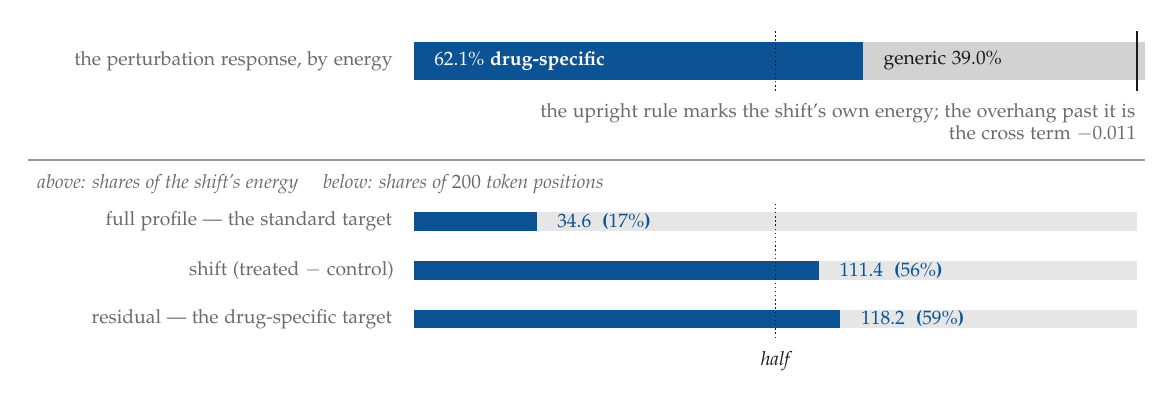
\begin{tikzpicture}[x=1cm, y=1cm, font=\small]
  \def\X{4.900}                  % left edge of every bar
  \def\L{9.190}                  % bar length for 100%
  \newcommand{\bx}[1]{\X+#1*\L}  % value -> x   (no braces: see header)
  % PIN THE BOUNDING BOX. Left free, the picture measures 409.59pt and runs
  % 5.56pt over the block: the rowname nodes are anchor=east at 4.75 with a
  % 4.65cm text width, so their inner sep hangs ~0.09cm left of x=0, and the
  % "half" descender hangs below. Neither carries ink -- the row labels are
  % flush right and set single-line, so their ink starts at x=0.07cm. Pinning
  % to [0, \bx{1.011}] therefore clips nothing and makes the drawn width equal
  % the stated 14.191cm = 403.775pt exactly.
  \useasboundingbox (0,-0.25) rectangle ({\bx{1.011}},4.12);
  \tikzset{
    rowname/.style={anchor=east, text width=4.65cm, align=flush right,
                    font=\scriptsize, text=quietink},
    inlab/.style={anchor=west, font=\scriptsize\bfseries, text=white},
    outlab/.style={anchor=west, font=\scriptsize\bfseries, text=accent},
    greylab/.style={anchor=west, font=\scriptsize, text=ink}}

  % ========== SUB-BLOCK 1: the response, by energy. Bars 4.8mm. ============
  \node[rowname] at (4.75,3.70) {the perturbation response, by energy};
  \fill[accent]      (\X,3.46)          rectangle (\bx{0.621},3.94);
  \fill[rulegrey!45] (\bx{0.621},3.46)  rectangle (\bx{1.011},3.94);
  \node[inlab]   at ({\X+0.14},3.70)          {$62.1\%$ drug-specific};
  \node[greylab] at ({\bx{0.621}+0.14},3.70)  {generic $39.0\%$};

  % the shift's own energy, and the cross term as the overhang past it
  \draw[ink, line width=0.7pt] (\bx{1.0},3.32) -- (\bx{1.0},4.08);
  \node[anchor=north east, text width=7.6cm, align=flush right,
        font=\scriptsize, text=quietink] at ({\bx{1.011}},3.28)
    {the upright rule marks the shift's own energy; the overhang past it is
     the cross term $-0.011$};

  % --- the divider: the two sub-blocks are different quantities ------------
  \draw[rulegrey, line width=0.4pt] (0,2.44) -- ({\bx{1.011}},2.44);
  \node[anchor=north west, font=\scriptsize\itshape, text=quietink] at (0,2.38)
    {above: shares of the shift's energy \quad below: shares of $200$ token
     positions};

  % ========== SUB-BLOCK 2: the target, by token position. Bars 2.4mm. ======
  % r1 -- the standard target
  \fill[rulegrey!25] (\X,1.54) rectangle (\bx{1.0},1.78);
  \fill[accent]      (\X,1.54) rectangle (\bx{0.17},1.78);
  \node[rowname] at (4.75,1.66) {full profile --- the standard target};
  \node[outlab]  at ({\bx{0.17}+0.14},1.66) {$34.6$ \;($17\%$)};

  % r2 -- the shift
  \fill[rulegrey!25] (\X,0.92) rectangle (\bx{1.0},1.16);
  \fill[accent]      (\X,0.92) rectangle (\bx{0.56},1.16);
  \node[rowname] at (4.75,1.04) {shift (treated $-$ control)};
  \node[outlab]  at ({\bx{0.56}+0.14},1.04) {$111.4$ \;($56\%$)};

  % r3 -- the residual
  \fill[rulegrey!25] (\X,0.30) rectangle (\bx{1.0},0.54);
  \fill[accent]      (\X,0.30) rectangle (\bx{0.59},0.54);
  \node[rowname] at (4.75,0.42) {residual --- the drug-specific target};
  \node[outlab]  at ({\bx{0.59}+0.14},0.42) {$118.2$ \;($59\%$)};

  % --- the half-way rule, drawn LAST so the bars do not bury it, and drawn
  % ONLY within the two bar bands so it crosses no prose. See header.
  \draw[ink, line width=0.5pt, densely dotted] (\bx{0.5},3.32) -- (\bx{0.5},4.08);
  \draw[ink, line width=0.5pt, densely dotted] (\bx{0.5},0.18) -- (\bx{0.5},1.90);
  \node[anchor=north, font=\scriptsize\itshape, text=ink] at (\bx{0.5},0.14) {half};
\end{tikzpicture}
\caption[The drug is most of the response, little of the
target]{\textbf{The drug is the majority of the perturbation response and almost
none of the standard target's tokens.} Above the rule: the shift's energy
decomposes exactly into a drug-specific residual, a generic programme and a
cross term, so $62.1\%$ of what a perturbation does to a cell is specific to
the compound. Below it: of the $200$ positions a cell sentence spends on the
standard target, only $34.6$ carry a different gene for two drugs in the same
context --- the other $83\%$ are the same string. Ranking the same measurement
by signed residual raises that to $118.2$, and at the plate scope this build
trains in the residual row reads $120.3$ ($60\%$). The two halves of the figure
are different quantities, an energy share and a count of token positions; they
share the axis and the half-way rule and nothing else, and no difference
between them is a number. What the picture states is an ordering: the signal is
a majority of the response, the standard encoding exposes a small minority of
it to the loss, and the residual encoding puts the exposed fraction back on the
majority side (\cref{tab:divergence}).}
\label{fig:residual-energy}
\end{figure}


That share has not previously been computed for this task, and its frame is not
the trained-on one. The stored generic averages over conditions and keeps the
condition's own contribution, where the training frame averages over drugs and
leaves the condition's own drug out. Self-inclusion scales a residual by
$(m-1)/m$ in a plate group of $m$ conditions, so that frame difference depresses
the share quoted here; it does not inflate it. The weighting difference has no
established direction. A second bias runs the other way. A condition's pseudobulk
sampling error enters its own shift whole and is averaged down in the group mean,
so it lands in the residual term and inflates the estimated share at this cell
budget (\cref{tab:scale}, and the reliability line above). The two oppose each
other, the net is not established, and no noise-corrected share is estimated
here.

\paragraph{Two components ask for different work} Writing
\begin{equation}
 \resid(d,c) \;=\; \beta(d) \;+\; \kappa(d,c) \;+\; \epsilon,
 \qquad
 \Tcoef \;=\; \frac{\operatorname{var}\beta}{\operatorname{var}\beta + \operatorname{var}\kappa},
\end{equation}
the per-drug constant $\beta(d)$, the drug \emph{main effect}, is what a lookup
table reproduces with no model at all.\seealso{\cref{sec:res-lookup} builds that
lookup and scores it.} The remainder $\kappa(d,c)$ is the only component a
conditional model could win on. This is DrEval's naive predictor~\cite{dreval} in
transcriptomic space. Their \texttt{NaiveMeanEffectsPredictor} predicts
$\hat{y}_{ij} = \mu^c_i + \mu^d_j - \mu$, cell-line and drug main effects with no
interaction term, and $\textrm{generic}(c) + \beta(d)$ is that quantity lifted
from a scalar potency to a $946$-dimensional profile.

Two warnings attach before any number is quoted. $\kappa$ is written as a
drug\,$\times$\,cell-line interaction because the decomposition assumes one, but
the estimator used does not identify such a term, so $\kappa$ is called the
\emph{context-specific remainder} and $\Tcoef$ a disattenuated cross-context
residual-similarity coefficient, not a variance share. And $1 - \Tcoef$ does not
measure the headroom above the additive baseline. The cross-line pairs entering
it may also differ in dose and in treatment well, and each residual is taken
against a generic its own drug helped define, so it bounds that headroom from
above at best.

% PLACEMENT: this box carries a display equation and cannot break usefully. At
% the previous setting it opened at the foot of the page and tcolorbox broke it
% immediately after the title bar, stranding "DEFINITION The transfer
% coefficient" alone at the page bottom with every line of the body overleaf.
% \budgettick's own \needspace{5\baselineskip} is not enough to catch that; the
% box is ~13 lines tall, so ask for that and let it move whole.
\needspace{12\baselineskip}
\begin{defn}{The transfer coefficient}
With $\num{286}$ of $\num{287}$ treatments in exactly one well there is
no replicate from which to separate $\operatorname{var}\kappa$ from
$\operatorname{var}\epsilon$, so the variance-components model is unidentified on
its own. The cosine route buys identification through split-half reliability:
\begin{equation}
 \hat{\Tcoef} \;=\; \frac{\cos\!\big(\resid(d,c_1),\, \resid(d,c_2)\big)}
 {\sqrt{\rho(d,c_1)\,\rho(d,c_2)}},
 \qquad
 \rho(d,c) \;=\; \frac{2\cos(\resid_A, \resid_B)}{1 + \cos(\resid_A, \resid_B)},
\end{equation}
where $\resid_A$ and $\resid_B$ are disjoint halves of condition $(d,c)$ and
$\rho(d,c)$ is the Spearman--Brown reliability of that condition's residual at
its full cell count.
\end{defn}

Dividing out the reliability is essential, since measurement noise alone
depresses the raw cross-line cosine and would otherwise be read as interaction.
Two cautions ride with it. Spearman--Brown is derived for correlations between
parallel halves, and what licenses it on a cosine here is the planted-truth
validation in \cref{sec:appendix}. And the reliability entering it is a
within-well split-half precision, optimistic relative to true biological
reproducibility. That optimism sits in the denominator, where an over-large
$\rho$ makes $\hat{\Tcoef}$ too small, so $1 - \hat{\Tcoef}$ is, if anything,
\emph{overstated}. An earlier draft had that direction the wrong way round.

\paragraph{The control that had to be replaced} The first run compared $\Tcoef$
against a negative control of different drugs on the same plate, which returned
$+0.485$ against $\Tcoef = 0.511$, and was correctly declared
void.\corrmark{the same-plate negative control is voided, not matched; the
structure-matched control replaces it} That control differs from the estimand in
two ways at once, different drug \emph{and} same cell line, and plate structure
surviving a cell-line-scoped generic inflates same-plate comparisons while
leaving cross-line comparisons untouched. The $+0.485$ is voided, not matched
against the separate $-0.017$ plate-scoped diagnostic. Only a structure-matched
control, breaking the drug match alone, bounds the estimand.

% ...........................................................................
\begin{table}[htbp]
\begin{threeparttable}
\caption{\textbf{The five checks accompanying the transfer-coefficient
estimate, and what each one bounds.} At $\kappa = 0$ the \emph{uncorrected}
cross-line cosine is only $0.734$, which read naively reports $27\%$ interaction
where the truth is zero, while the disattenuated estimator recovers the truth to
within $0.001$. That recovery licenses the reference column of
\cref{tab:transfer}.}
\label{tab:tcontrols}
\small
\begin{tabularx}{\linewidth}{@{}>{\raggedright\arraybackslash}p{0.34\linewidth}X@{}}
\toprule
\thead{Check} & \thead{What it bounds} \\
\midrule
disjoint control halves & shared-control inflation: $+0.242$ at cell-line scope,
  $-0.000$ at plate \\
structure-matched negative control & the estimand itself; returns $-0.008$ \\
simulated $\kappa{=}0$ null & estimator bias: returns $1.001$ where the truth is
  $1.000$ \\
dose strata on molar doses & a reference scale: the same drug and line at
  another dose \\
leave-one-drug-out generic & train/held-out target asymmetry
  (\cref{sec:methods-residual}) \\
\bottomrule
\end{tabularx}
\begin{tablenotes}[flushleft]\footnotesize
\item An earlier cache carried the well identifier in the dose field, so what was
labelled dose transfer compared physical wells, not concentrations.
\end{tablenotes}
\end{threeparttable}
\end{table}

% ...........................................................................
\begin{table}[htbp]
\begin{threeparttable}
\caption{\textbf{The transfer coefficient, estimated on real molar doses with
dyadic cluster-robust intervals.} The matched negative control sits on zero. The
same-plate control that produced the earlier false alarm reads $+0.485$ under a
cell-line-scoped generic. $\Tcoef$ is a cross-context similarity coefficient, not
a variance share, and $1 - \Tcoef$ must not be read as a
drug\,$\times$\,cell-line interaction share.}
\label{tab:transfer}
\small
\begin{tabularx}{\linewidth}{@{}%
  >{\raggedright\arraybackslash}p{0.28\linewidth}
  >{\raggedright\arraybackslash}p{0.13\linewidth}
  >{\raggedright\arraybackslash}p{0.20\linewidth}
  >{\raggedright\arraybackslash}X@{}}
\toprule
\thead{Quantity} & \thead{Estimate} & \thead{$95\%$ interval} & \thead{Reference} \\
\midrule
$\Tcoef$ (cross-context, plate-scoped generic) & $0.553$ & $[0.514, 0.593]$
  & simulated $\kappa{=}0$ null $= 1.001$ \\
similarity scale NOT shared across contexts, $1-\Tcoef$ & $44.7\%$
  & $[40.7\%, 48.6\%]$ & mixes cell line, dose, well and estimator \\
$\Tcoef$ across dose (same drug, same line) & $0.707$ & $[0.632, 0.782]$
  & reference scale \\
structure-matched negative control & $-0.008$ & spanning zero
  & must be $\approx 0$ \\
\bottomrule
\end{tabularx}
\end{threeparttable}
\end{table}

\paragraph{What the coefficient is, precisely} $\Tcoef$ is a descriptive
sensitivity analysis and not a load-bearing estimate, and the reason sits in its
configuration. The scoped calculation retains conditions at a reproducibility
threshold of $0.2$, and it carries every caution above at once: a
\emph{self-including} generic, pairs free to differ in \emph{dose} and in
treatment well, and an optimistic reliability in the denominator. That last one
pushes $\hat{\Tcoef}$ down, so $1 - \Tcoef$ errs high and bounds from above what
a per-drug constant leaves on the table, without measuring it.

\paragraph{Dose is the milder perturbation} Holding drug and cell line fixed and
changing only the molar concentration, transfer is $0.707$ $[0.632, 0.782]$ on
$\num{363}$ pairs against $0.553$ $[0.514, 0.593]$ pooled cross-context; the
intervals do not overlap. That contrast is between one clean axis and a mixture,
since the cross-context arm differs in well and dose as well as cell line, but it
is the closest this section comes to a single-axis comparison.

The same ordering served as the weaker of the two scope diagnostics. At cell-line
scope it inverts. The dose arm falls to $0.4846$, a different quantity from the
voided same-plate control, which coincidentally reads $0.4853$, while the
cross-line coefficient holds at $0.511$. That is the wrong way round for dose
against cell line, but the expectation is a prior, so it is used as a
plausibility check. The second diagnostic needs no prior. At plate scope the
shared-control and split-control builds of $\Tcoef$ agree to $-0.000$, while at
cell-line scope they differ by $+0.242$, plate structure leaking through a
cell-line-scoped generic. That is what the scope decision rests on, and it is why
the cell-line-scoped build cannot corroborate when it returns a similar
$\Tcoef = 0.511$; that build is the one declared void, its own same-plate
negative control reading $+0.485$.

\paragraph{Whether anything could learn the remainder} If a cell line modulated
drug responses in a consistent direction, that direction would be estimable from
the line's own cells. Writing $\kappa(d,c) = \resid(d,c) - \hat{\beta}(d)$, the
test compares $\cos(\kappa(d,c), \kappa(d',c))$ for different drugs in the same
cell line against the same quantity across different cell lines, with
$\hat{\beta}$ estimated leave-one-cell-line-out; estimated over all lines it
would contain $\resid(d,c)$ itself, and subtracting a mean containing its own
term induces a $-1/(m-1)$ correlation that biases the signal arm downward by
construction. Both arms are disattenuated by $\kappa$'s own split-half
reliability.

Averaged over lines, no consistent per-line direction shows up. Under the
plate-scoped generic the same-cell-line arm reads \ci{-0.0149}{-0.0251}{-0.0050}
and the different-cell-line arm \ci{+0.0003}{-0.0071}{+0.0081}, an excess within
line of $-0.0153$ for which no interval was computed. The intervals come from a
cell-line-clustered bootstrap over $\num{38}$ and $\num{42}$ clusters, on
$\num{4000}$ same-line and $\num{3884}$ cross-line pairs over $\num{1282}$
conditions. Neither arm shows the positive within-line excess a per-line
direction would require, and the negative sign of the same-line arm is not read
as evidence: same-line pairs that also share a plate share a generic, and that
common subtraction pushes their cosines negative by construction, where
cross-line pairs share no generic at all. It is the construction the
different-drug same-plate diagnostic reads at $-0.017$ above. A
cell-line-scoped counterpart was not computed in the canonical run, and the row
an earlier draft carried for it is withdrawn.

Two negative results do not add up to irreducibility: this one, and a direct
test of whether mechanism-matched drugs deviate from their per-drug constants in
the same way within a cell line, which returned nothing detectable. The second
bounds its own power severely. $\kappa$'s split-half reliability in this atlas is
$0.195$ at the $0.05$ reliability floor ($0.324$ at the stricter $0.20$ floor),
and same-mechanism drugs are so heavily co-plated that only $3$--$7\%$ of
matched pairs survive a different-plate requirement ($1\%$ at the stricter
floor). Resolving $\kappa$'s structure would take more cells per condition or a
plating design that crosses mechanism with plate.

\begin{claim}
There is a conditional target that a per-drug constant cannot express. Two tests
looked for learnable structure in it and found none, and neither settles whether
there is any. $\kappa$'s split-half reliability is $0.195$ at the floor the
mechanism test runs at, and only $3$--$7\%$ of mechanism-matched pairs survive a
different-plate requirement, so its structure is unresolved here rather than
\shownzero. Its size is quoted as what it is: $\Tcoef = 0.553$
\nolinebreak[3]$[0.514, 0.593]$ is a disattenuated cross-context similarity
coefficient, so $44.7\%$ $[40.7\%, 48.6\%]$ of \emph{that similarity scale}
remains unshared across the compared contexts. It is not a variance share and not
a drug\,$\times$\,cell-line interaction, since the estimator pools pairs
differing in cell line, dose, well and target estimator, so it bounds what a
per-drug constant leaves on the table without establishing that a model could
reach any of it.
\end{claim}

% ...........................................................................
\beatsection{R}{5}{Re-encoding produces prompt sensitivity}{sec:res-encoding}

\begin{question}[5]
Every target change tried so far left the model indifferent to the drug named in
its prompt. Does training on the residual change that? The instrument is the
stratified scramble, the same prompt with another drug's name and mechanism
substituted, read as a ladder of strata because the swapped-in drug is itself a
drug the model knows and so is not a neutral comparison. The model moves. It is
not the only target change that makes it move.
\end{question}

\noindent
On the $\num{300}$ trained conditions of the residual-frame evaluation the model
beats the geometry-defined \texttt{orth} scrambled partner by
\ci{+0.0898}{+0.0291}{+0.1506}, clustered on the drug and the treatment well
(\texttt{re\_v3.json}).\gloss{scramble}{The same prompt with the drug's name and
mechanism replaced by another drug's, in three strata by residual similarity.}
That is the first non-null drug effect in this project, first in the order the
experiments were run, and not the only target construction that produces one.

% ...........................................................................
\paragraph{Why the comparison set is not exchangeable, and what follows} The
comparator is not a null. Its own score is a monotone function of which drug it
was handed, which makes it an active treatment; \cref{sec:res-generalisation}
measures the size of that. Two consequences fix the reading protocol here. The
series is quoted as a \emph{gradient}, since a metric artefact would not order
itself by swap dissimilarity; and where a single magnitude is needed it is the
\texttt{orth} one, the least contaminated comparison available and not an
independently established null, that stratum having been defined using true
residual geometry.

\paragraph{Why the strata are cut by response geometry and not by mechanism} A
scramble that swaps in a drug with a similar true response is a weak test, and
the annotation that looks like it should prevent that does not. In the
characterisation behind \cref{tab:scale}, two drugs sharing a \texttt{moa-fine}
annotation sit a mean distance $2.322$ apart against $2.377$ for two drugs that
do not, $\num{1244}$ same-mechanism against $\num{17563}$ different-mechanism
pairs, a ratio of $0.977$. Same-mechanism drugs in Tahoe are just over two per
cent closer to each other than arbitrary pairs are, so ``different mechanism''
does not imply ``different response''. The strata are therefore cut by measured
residual cosine within the cell line. (Mechanism does carry signal in the
residual frame, \cref{sec:res-scope}, a different frame from the full profiles
measured here.)

\paragraph{The gradient, on the earlier target build} The stratified scramble of
\cref{sec:methods-controls} gave a gap that grew with swap dissimilarity
(\cref{fig:repair}), \ci{+0.0351}{+0.0061}{+0.0656},
\ci{+0.0716}{+0.0371}{+0.1059} and \ci{+0.1429}{+0.1112}{+0.1787}
across \texttt{near}, \texttt{orth} and
\texttt{opposite}, each differenced against its own stratum-specific partner.
These are the residual arm's $1400$-token run; the two control arms beside them
were scored at the $600$-token cap of \cref{sec:methods-data}, where their
stratum gaps run from $-0.021$ to $+0.026$ and were read at the time as flat and
null. That reading holds for the single-cell arm at both budgets. It does not
hold for the optimal-transport arm, whose $600$-token gaps are themselves
monotone in swap dissimilarity.

\begin{figure}[htbp]
\centering
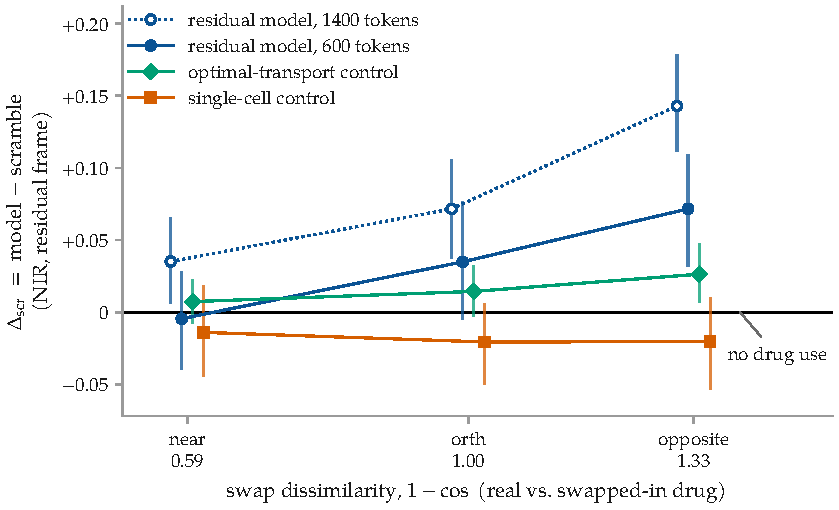
\includegraphics{fig-repair}
\caption[The gap grows with swap dissimilarity]{\textbf{On the earlier target
build, the residual model's advantage over its own scramble grew with how
dissimilar the swapped-in drug's residual was; the single-cell control scored
through the identical pipeline stayed flat and null, while the optimal-transport
control did not.} Residual frame throughout. The horizontal axis is measured
swap dissimilarity, $1-\cos$ between the real and the swapped-in drug's residual,
byte-identical across all four runs, so the three stratum positions are exact;
the connecting lines are guides between three measured strata and not a sampled
continuum, and the four series are nudged sideways so that their intervals do not
overlap. The three solid series are at a matched $600$-token
budget; the residual model's $1400$-token run is the dotted overlay, since the
budget alone roughly doubles the gap on the two strata where it is positive at
$600$ ($+0.0349 \rightarrow +0.0716$ on \texttt{orth},
$+0.0716 \rightarrow +0.1429$ on \texttt{opposite}). Intervals are $95\%$
bootstrap clustered over cell lines, $n = 250$ conditions per point. The
\texttt{near} stratum is the weakest test by construction, since where the
swapped-in drug's true residual is similar, an unchanged prediction is correct.}
\label{fig:repair}
\end{figure}

\paragraph{Three diagnostics that need no scramble} All three agreed on that
build, and the residual model led on all three. The correlation between a
condition's reproducibility and model $\NIR$ was $+0.144$, the model doing better
where the drug effect is real, against $-0.117$ and $-0.216$ for the controls.
Prediction diversity was highest for the residual model. And
$\cos(\textrm{prediction}, \textrm{own truth})$ exceeded
$\cos(\textrm{prediction}, \textrm{other drugs})$ for all three arms, the
residual model's margin, $+0.084$, being roughly twice the optimal-transport
arm's $+0.049$ and three times the single-cell arm's $+0.026$.

\paragraph{One measurement lesson before the withdrawal} The $600$-token cap
roughly halved the effect at every stratum where it was positive there, so
$+0.0716$ appears twice in this section, once as the $600$-token
\texttt{opposite} gap and once as the $1400$-token \texttt{orth} gap, and the two
are not the same quantity. Re-run at $1400$ tokens, the single-cell control stays
flat, $-0.0128$ \nolinebreak[3]$[-0.0458, +0.0202]$ against its own
\texttt{orth} partner. The optimal-transport control does not.

% PLACEMENT ONLY. Worst case of the breakable box: nine lines of the retraction
% at the foot of one page, then \cref{fig:repair} taking the whole top of the
% next as a deferred float, then the remaining six lines under it -- the box read
% as two boxes with a figure between them. 17 lines is the box entire, so it
% either sets whole here or starts the next page whole, and the figure can no
% longer land inside it.
\needspace{17\baselineskip}%
\begin{withdrawn}{``OT achieved nothing'', \cref{sec:res-epsilon}}
At $600$ tokens the optimal-transport arm's \texttt{orth} gap was
\ci{+0.0144}{-0.0051}{+0.0338} and spanned zero; at $1400$ it is
\ci{+0.0292}{+0.0144}{+0.0441} and does not. The token budget was suppressing a
real effect in that arm, the same lesson the residual arm taught, applied to a
control previously read as inert. The $600$-token evidence pointed the same way
and was read too cautiously; that arm's stratum gaps there were $+0.0073$,
$+0.0144$ and $+0.0263$, monotone in swap dissimilarity like the residual arm's,
with only \texttt{opposite} excluding zero. The consequence reaches backwards.
The optimal-transport target is one point in the three-point comparison of
\cref{sec:res-epsilon}, and that negative holds only at the budget and comparator
it was measured with. At a matched budget and against the geometry-defined
\texttt{orth} partner, whose true residual is on average orthogonal to the
target's ($\cos = +0.035$), the optimal-transport point is not null. The
single-cell point is the one whose interval still spans zero. The geometry-based
selection does not independently establish a null in either case.
\end{withdrawn}

\paragraph{The comparison that costs this section its strongest phrasing} The two
arms' pooled gaps against their own \texttt{orth} partners overlap almost
entirely (\texttt{ctrl1400\_summary.json}), so re-encoding the target produces
prompt sensitivity but is \emph{not} the only target change that does.

Three limits stop that comparison being read as an ordering. The arms are scored
in different frames, so only each arm's gap against its own comparator is
comparable; they are separate evaluations over different condition sets, so this
is an arm-level and not a paired comparison; and those sets differ in split
composition by more than the arms differ from each other. The residual figure
pools the three splits of \cref{tab:generalisation}, whose own gaps are
$+0.0898$, $+0.0332$ and $-0.0315$, while the optimal-transport evaluation
carries no split labels at all. A spread of that size across splits, against a
$0.0069$ difference between the two pooled numbers, means the near-equality does
not order the arms in either direction.

\paragraph{The slope carries its own null} Regressing each prediction's $\NIR$
on the cosine between the named drug's truth and the target's truth gives a
slope whose null is zero for a model that ignores the drug it is told. Its
points are the three scrambled partner prompts and nothing else, the target-drug
prompt never among them, and \cref{sec:res-generalisation} fits it on all three
splits. The fit is pooled least squares over every point in a split with a
single intercept, three points per condition, no condition-level intercepts
absorbed, so the zero null is exact within a condition while the pooled slope
also carries a between-condition component. What it closes is the freedom to
pick a comparator, since it spends all three strata rather than one.

\begin{claim}
Re-encoding the target produced the project's first non-null drug effect. On
trained conditions the model beats the geometry-defined \texttt{orth} partner by
\ci{+0.0898}{+0.0291}{+0.1506} and beats chance outright, with no comparator arm
at all, by \ci{+0.0981}{+0.0407}{+0.1554}, both clustered on the drug and the
treatment well, the drug being the axis the claim rides on
(\cref{sec:res-generalisation}). The comparator-free slope of retrieval against
the named drug's truth is \ci{+0.3728}{+0.2797}{+0.4660}, and zero is its null for a
drug-blind model, so no choice of comparator manufactures it, though it is fitted over the
scrambled partner prompts alone, with the target-drug prompt never a point on the
line. It is first in sequence and not uniquely responsible: at a matched
$1400$-token budget the optimal-transport target clears zero against its own
\texttt{orth} partner too (\ci{+0.0292}{+0.0144}{+0.0441} over $\num{248}$
conditions that carry no split labels, against the residual arm's
\ci{+0.0361}{+0.0159}{+0.0564} pooled over $\num{1394}$ that mix trained and
held-out splits), on a separate evaluation in a different frame, so the two are
not ordered against each other. The model has been shown to respond to the drug;
whether that response is any use is the next question.
\end{claim}

% ...........................................................................
\beatsection{R}{6}{Responding to the drug is not predicting it}{sec:res-generalisation}
\label{sec:methods-holdout}

\begin{question}[6]
A model that moves when the drug token moves has cleared a low bar, because
reproducing a training average requires that much too. Everything scored so far
came from conditions the model trained on, so what has been shown is that the
token is consulted, not that anything transferable was learned. Separating the
two needs a holdout, and the
atlas's own randomisation decides which one means anything: whole treatment
wells. Prompt sensitivity survives that test. Whether the residual itself
transfers comes back unsettled.
\end{question}

\noindent
The physical layout of \cref{sec:methods-data} forces the choice. A (drug, cell
line) holdout, the field's standard Leave-Pairs-Out split and the one an earlier
version of this work used, leaves the held-out condition's treated well sitting
in the training set through its other $\approx 48$ cell lines. Measured against
that holdout, $\num{124}$ of the $\num{255}$ treated wells for which split
information exists placed a held-out condition and a training condition in the
same well.\seealso{\cref{sec:res-lookup}: what a held-out gap has to
beat.} That estimand measures within-atlas matrix completion, not independent
generalisation, and no processing of the targets changes it.

Holding out whole wells is the only assignment-respecting choice the design
offers, and it answers a narrower question, generalisation to an unseen treatment
well of a seen drug. Fixed-dose cross-context transfer, present in one line and
absent in another, is structurally unidentifiable in this atlas.

\paragraph{What each split holds} \texttt{train} takes every condition of the
remaining wells, $\num{4999}$ before the reliability line and
\needsaudit[tally against the gate's retained count]{2{,}523} after it.
\texttt{unseen\_combo} holds $\num{36}$ treated wells out whole ($\num{904}$
conditions, $\num{900}$ after inventory filters), and it never takes a drug's
last training well; without that guard a two-well drug could silently become an
unseen drug while sitting in the unseen-combination arm, and the two arms would
measure the same thing. \texttt{unseen\_drug} holds every condition of
$\num{10}$ held-out drugs ($\num{714}$ conditions, $\num{711}$ after inventory
filters). Zero wells contribute conditions to both sides.

\texttt{unseen\_drug} is a control and not a third result. Tahoe fine-tuning
never sees the token, so a large effect there would indict the comparator, not
report a biological finding. ``Unseen'' means held out from fine-tuning with
mechanism supplied, not unknown to the pipeline; the Pythia-1b backbone was
pretrained on natural language and the prompt still carries the
\texttt{Mechanism:} field.

Two warnings ride with the design. DrEval reports, citing~\cite{partin}, that
apparently good performance on pair-holdout splits can be reached simply by
predicting each drug's average response across the training cell lines, which is
why the baseline ladder of \cref{sec:res-lookup} is not optional. And the
evaluation draws under a per-split quota, because a uniform draw reproduces the
pool's proportions and starves the split the experiment exists to test; in a
first run,
$\num{250}$ constructed held-out combinations yielded only $\num{33}$ scored
conditions. Under the quota the evaluation scores $\num{1394}$ conditions in all,
$\num{300}$ trained and $\num{199}$ unseen-drug, the rest unseen combinations,
almost the whole pool of $\num{900}$ that arm affords, while
\texttt{unseen\_drug} remains a quota of the $\num{711}$ available.

% ...........................................................................
\paragraph{The first result of this design is about the comparator} It is a
finding and not an erratum, and it reframes every gap quoted so far. Across the
three swap strata the scrambled model's $\NIR$ is $0.550$, $0.501$ and $0.423$ as
the named partner's true residual moves from aligned ($\cos = +0.22$) through
orthogonal ($0.00$) to anti-aligned ($-0.20$) with the target. The
\texttt{near} and \texttt{opposite} scores differ from chance in opposite
directions; the geometry-defined \texttt{orth} partner scores $0.501$ and is
empirically near chance on these conditions. That makes \texttt{orth} the least
contaminated available comparator, not an independently established null, since
its stratum was defined using true residual geometry.

The consequence is structural. A gap measured against such an arm decomposes as
\begin{equation}
 \gap \;=\; \underbrace{\big(\NIR_{\textrm{model}} - 0.5\big)}_{\textrm{how much naming the truth helps}}
 \;+\; \underbrace{\big(0.5 - \NIR_{\textrm{scramble}}\big)}_{\textrm{how much naming the lie hurts}},
\end{equation}
and only the first term is wanted. The second is not a rounding error. Pooled
over all $\num{1394}$ scored conditions the model's own advantage over chance is
$+0.0367$ and the \texttt{opposite} comparator's deficit is $+0.0772$, so $68\%$
of the $+0.1139$ gap that arm reports is the comparator failing and not the model
knowing. Against \texttt{orth} the second term is approximately zero here, so
every gap in \cref{tab:generalisation} is measured against that partner, its
magnitude conditional on the observed near-chance score.

The diagnostic is free and not specific to this experiment. Score the comparator
arm against chance; if its score moves with which label it was handed, the gap it
defines is not a measurement of the model. A swap drawn to be maximally
dissimilar, the obvious way to build a strong negative control, is exactly the
swap that maximises the second term.

% ...........................................................................
\begin{table}[htbp]
\begin{fullwidth}
\begin{threeparttable}
\caption{\textbf{Whole-well holdout on the corrected evaluation, with the truth
verified against the build's own fit digest and the full held-out population
scored.} The two right-hand columns carry the SAME point estimate and differ only
in what they treat as the unit of generalisation. On \texttt{unseen\_combo} the
gap excludes zero clustered on cell line and does not clustered on drug, which is
why that row is reported as \notestablished. The \texttt{unseen\_drug} row
corroborates but does not prove: its \texttt{orth}-partner gap is negative while
its \texttt{opposite} gap is $+0.0379$.}
\label{tab:generalisation}
\small
\begin{tabularx}{\linewidth}{@{}%
  >{\raggedright\arraybackslash}p{0.16\linewidth}
  >{\raggedright\arraybackslash}p{0.18\linewidth}
  >{\raggedright\arraybackslash}p{0.16\linewidth}
  >{\raggedright\arraybackslash}X
  >{\raggedright\arraybackslash}X@{}}
\toprule
\thead{Split} & \thead{$n$ (lines; drugs; wells)} & \thead{model $\NIR$}
  & \thead{$\gap$, clustered on \emph{cell line}}
  & \thead{the same, clustered on \emph{drug}} \\
\midrule
\texttt{train} & $300$ ($39$; $76$; $136$) & $0.598$ $[0.549, 0.647]$
  & \ci{+0.0898}{+0.0382}{+0.1415} & \ci{+0.0898}{+0.0291}{+0.1506} \\
\addlinespace
\textbf{\texttt{unseen\_combo}} & \needsaudit{895} ($42$; $34$; $36$)
  & $0.533$ $[0.492, 0.575]$
  & \ci{+0.0332}{+0.0069}{+0.0594} & \ci{+0.0332}{-0.0031}{+0.0695} \\
\addlinespace
\texttt{unseen\_drug} & $199$ ($40$; $10$; $28$) & $0.459$ $[0.404, 0.514]$
  & \ci{-0.0315}{-0.0836}{+0.0206} & \ci{-0.0315}{-0.1049}{+0.0419} \\
\bottomrule
\end{tabularx}
\begin{tablenotes}[flushleft]\footnotesize
\item Every gap printed here is measured against the geometry-defined
\texttt{orth} partner, whose own score is empirically near chance on these
conditions; \texttt{opposite} figures never appear as a column. Model $\NIR$
intervals test against the chance value $0.5$ with no comparator. Intervals are
two-way cluster-robust over cell lines and wells, with a Student $t$ reference
on $\min(G_{\textrm{line}}, G_{\textrm{well}}) - 1$ degrees of freedom, which is
why the well counts are printed. The \texttt{unseen\_drug} arm spans $28$
wells, and $t_{27} = 2.05$ against $1.96$ widens its interval by five per cent
(\cref{sec:methods-data}).
\end{tablenotes}
\end{threeparttable}
\end{fullwidth}
\end{table}

\paragraph{The control behaves as the diagnosis predicts} The unseen-drug gap
against \texttt{opposite} is \ci{+0.0379}{-0.0083}{+0.0841}, positive where the
\texttt{orth}-partner estimate on the same conditions and predictions,
\ci{-0.0315}{-0.0836}{+0.0206}, is negative and covers zero as a control should.
That point estimate is the \texttt{unseen\_combo} gap with the sign reversed, so
the row is read as uninformative and not as a confirmed null. A cluster-robust
variance is asymptotic in the number of clusters, not conditions, and this arm
spans $40$ cell lines but only $28$ treatment wells, so its two-way variance is
carried on $27$ degrees of freedom. A cell-line-only cluster bootstrap puts the
\texttt{opposite} gap clear of zero at $[+0.0044, +0.0727]$; adding wells as the
second clustering axis returns it to zero, at the normal quantile as well as at
$t_{27} = 2.05$. What decides the row is the unit of clustering.

\paragraph{The held-out row settles prompt sensitivity only} On
\texttt{unseen\_combo} the gap clears zero clustered on cell line and well but
not clustered on drug and
well (\cref{fig:splits}a, right), so it survives only one of the two units the
claim needs. Drug is the axis
a claim about transferring a \emph{drug}-specific residual has to generalise
across, so
generalisation to an unseen treatment well of a seen drug is \notestablished.

\begin{figure}[htbp]
\centering
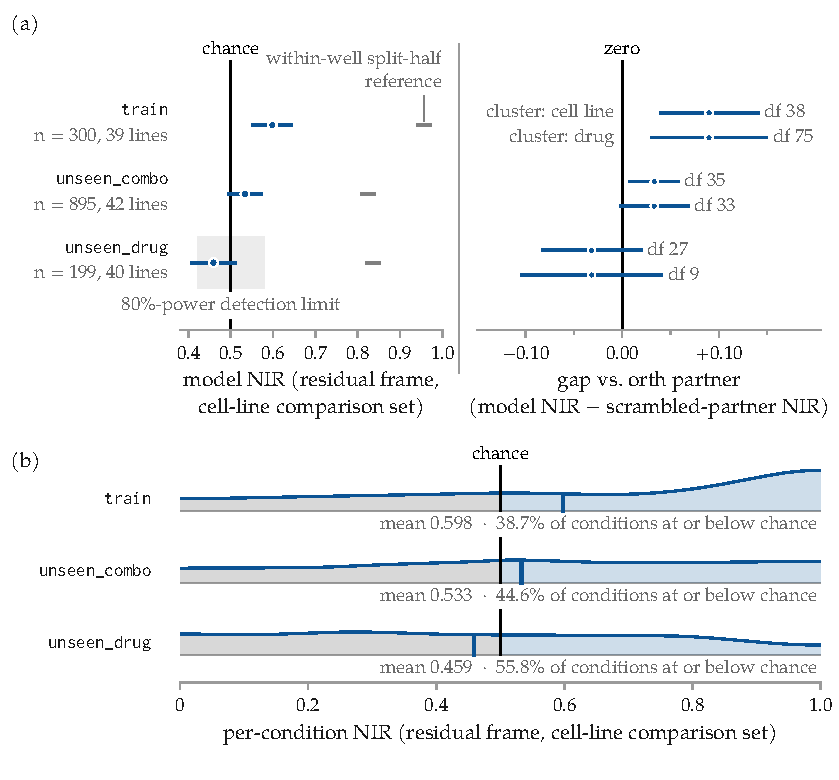
\includegraphics{fig-splits}
\caption[Chance-clearing on trained conditions only]{\textbf{The residual-frame
model clears chance on trained conditions only; the held-out-combination gap
excludes zero clustered on cell line but not clustered on drug, and the
unseen-drug gap flips sign.} Residual frame throughout, and $\NIR$ ranks each
prediction against the other drugs measured in the same cell line.
\textbf{(a)}~Left, model $\NIR$ against the chance value $0.5$ (solid rule), with
$95\%$ two-way cluster-robust intervals; $n = 300$, \needsaudit{895} and $199$ conditions on
\texttt{train}, \texttt{unseen\_combo} and \texttt{unseen\_drug}. The grey
dash on each row is that split's raw within-well split-half precision
reference, a measurement-precision figure computed from two halves of the same
well and not a replicate experiment; it carries no interval and is drawn as a
bare marker, and only \texttt{train} is filtered at the reliability line. Right,
on its own axis, the gap against the geometry-defined \texttt{orth} partner. Each
row has one point estimate, drawn twice with two intervals because the verdict
depends on which unit of generalisation is clustered: cell-line-clustered above,
drug-clustered below, each labelled with the Student~$t$ degrees of freedom it is
carried on. The grey band on the \texttt{unseen\_drug} row is that arm's
$80\%$-power detection limit around chance, $\pm 0.079$, the smallest departure
the arm could detect and not a confidence region. \textbf{(b)}~The per-condition
$\NIR$ distributions behind those three means, as reflected-boundary kernel
densities on a shared axis, each with its mean marked and the region at or below
chance shaded. The pooled $0.537$ is a mean over nearly flat distributions rather
than a location: even on \texttt{train}, $38.7\%$ of conditions sit at or below
chance, against $44.6\%$ and $55.8\%$ on the two held-out splits.}
\label{fig:splits}
\end{figure}

\begin{scopelimit}[carried into \cref{sec:res-lookup} and \cref{sec:limitations}]
The precision matters: \notestablished is not the same as \shownzero. The
drug-clustered interval reaches $+0.0695$, so an effect of up to roughly $+0.07$
remains compatible with these data at the
\needsaudit[arm size, two records disagree]{895} conditions this arm affords,
spread over $34$ drugs, a limit of power at the size the holdout gives,
reported as one. On \texttt{unseen\_drug}, $n = 199$ leaves a half-width of
$0.055$ around the model's own $\NIR$ and an $80\%$-power detection limit of
$0.079$ against chance, shaded on that row in \cref{fig:splits}a. Neither row
licenses a statement that the effect is absent.
\end{scopelimit}

% FLAGGED, NOT FIXED -- the two panel-B numbers below (train $0.955$ and the
% spread $0.006$) are inherited from a superseded reconstruction taken at a
% +0.109 reliability line. This document defines the line at +0.1086: see :214
% ("$+0.109$, resolving to $+0.1086$"), :222-223 ("none falls at or below the
% resolved $+0.1086$") and :986 ("499 conditions sit below the $+0.1086$ line").
% Recomputed from RESULTS_cluster/re_v3.json -> records[] at repro_cos > 0.1086:
%   train         kept 300  0.9555006 -> 0.956   (:222-223 requires all 300)
%   unseen_combo  kept 396  0.9605642 -> 0.961   (:986's 499-below requires 396)
%   unseen_drug   kept 111  0.9597734 -> 0.960
%   spread: raw 0.0050636 -> 0.005, and max(rounded) - min(rounded)
%           = 0.961 - 0.956 = 0.005. BOTH conventions give 0.005 at the resolved
%           line, so this is NOT the convention clash it was reported as. 0.006
%           is just the old line's rounded-endpoint spread, 0.961 - 0.955. At
%           0.109 the kept counts are 299 / 394 / 111, which contradict :222-223
%           and :986 directly.
% The $0.132$ in the same sentence is unaffected: panel A is read straight from
% CANONICAL_NUMBERS.json -> ceilings{}, and raw (0.13178) and rounded-endpoint
% (0.956 - 0.824) both give 0.132 there.
% NOT CHANGED HERE because the correction is a six-site edit and four sites are
% outside this file: 05-Limitations.tex:224 and :225, 03-Apparatus.tex:378, and
% figs/splitref.tex's spread node (:219) and caption (:244). That figure already
% DRAWS train as 0.956 at the resolved line while the prose here still prints
% 0.955, so the disagreement is live. Changing this site alone would replace a
% uniformly wrong number with an inconsistent document. Reported upward instead.
The three splits are not scored on comparable populations either, and the
difference is one of selection. Their raw within-well split-half precision
references, the grey dashes of \cref{fig:splits}a, are $0.956$, $0.824$ and
$0.836$, a spread of $0.132$; \texttt{train}
is filtered at a reliability line the two held-out splits are not, and imposing
that line on all three brings the references to $0.955$, $0.961$ and $0.960$, a
spread of $0.006$. The held-out shortfall therefore cannot be softened by appeal
to a lower noise floor.

% PLACEMENT ONLY. The other retraction in this section is guarded at the
% \needspace above; this one was not, and it broke 13 lines / 2 lines across the
% page. The two lines that landed overleaf are the ones that perform the
% withdrawal, and they arrived with no CORRECTION rule above them, so the reader
% met the retraction as unlabelled prose. \budgettick reserves 5\baselineskip,
% which is not enough: the box measures 247.1pt, 16.6 lines with its padding and
% frame, so 17 is the box entire and it either sets whole here or starts the
% next page whole.
% MEASURED COST, build of 2026-08-12: the guard carries ~2.6 lines of the
% chapter forward. That stops the closing claim of \cref{sec:res-lookup}
% breaking, and starts the coverage definition and the seen-drug-transfer claim
% breaking, all three in 04d-baselines.tex, each of which wants the same guard.
\needspace{17\baselineskip}%
\begin{withdrawn}{a training-exposure or memorisation advantage}
The difference between the trained and held-out estimates is
\ci{+0.0567}{-0.0014}{+0.1148} with cluster-robust $p = 0.0556$. An unclustered
permutation returns $p = 0.0142$, quoted only for contrast, because ignoring the
clustering this chapter mandates everywhere else flatters the result. It does
not clear the conventional threshold, and the two arms differ in three ways at
once in any case, in whether the condition was trained on, in which drugs they
contain, and in how their scored populations were selected. Restricting the
comparison to the $30$ drugs present in both arms reverses the sign, with the
trained arm sitting \emph{behind} the held-out one,
\ci{-0.0606}{-0.1506}{+0.0295}, $p = 0.1797$, on $79$ trained and $750$
held-out conditions, and the pooled difference is a composition effect: $83.8\%$
of held-out-combination conditions sit on those shared drugs against $26.3\%$
of trained ones. The claim of a training-exposure or memorisation advantage is
therefore withdrawn. None is established, the drug-matched estimate points the
other way, and the two arms are scored on populations selected by different
rules.
\end{withdrawn}

\paragraph{Two instruments no comparator defect can touch} First, the slope test.
Regressing each prediction's $\NIR$ on the cosine between the named drug's truth
and the target's truth gives \ci{+0.373}{+0.280}{+0.466} on \texttt{train},
\ci{+0.336}{+0.223}{+0.450} on \texttt{unseen\_combo} and
\ci{+0.342}{+0.215}{+0.469} on \texttt{unseen\_drug}, clustered on the drug. All
three exclude zero, and all three still exclude it clustered on the cell line
($[+0.272, +0.474]$, $[+0.241, +0.432]$ and $[+0.284, +0.400]$). Its points are
the three \emph{scrambled} partner prompts and nothing else, exactly three per
condition, so $900$, $\num{2685}$ and $597$ points on the three splits. On
\texttt{unseen\_drug} those partners are overwhelmingly drugs the model
\emph{was} trained on, so the slope shows that the model responds to a named
trained drug in a scoring context whose own drug was held out, and not that it
knows the held-out drug.

Second, the model's own score against chance, with no comparator at all. It
clears $0.5$ on \texttt{train}, by $+0.0981$
\nolinebreak[3]$[+0.0407, +0.1554]$ clustered on drug and well, and is not
distinguishable from chance on either held-out split
(\cref{tab:generalisation}).

\paragraph{A positive slope beside a chance-level score is not a contradiction}
The model has a coarse sense of what a named trained drug does, and not of what
it does in this well, and $\NIR$ asks the second question, ranking against the
$\approx 40$ other drugs in the same cell line. That is the drug main effect
without the part of the residual that is not shared across contexts, which
\cref{sec:res-transfer} measures at $44.7\%$ ($1 - \Tcoef$, with
$\Tcoef = 0.553$ \nolinebreak[3]$[0.514, 0.593]$), a figure that mixes cell line,
dose, well and estimator. It is also why the lookup wins in the next section:
\texttt{drug\_lookup} is that main effect, estimated straight from data far more
precisely than the model learned it. The condition-level picture agrees. The
cosine between prediction and own truth on trained conditions averages $+0.0389$
(sd $0.1119$, median $+0.0220$), spanning $[-0.3046, +0.3976]$ with $33.7\%$
clearing $|0.1|$.

\paragraph{One asymmetry attaches to every held-out number in this chapter} The
evaluation's truths are not refitted. The generic is reconstructed from the
build's own fit inventory and verified against the build's \texttt{fit\_digest},
and a mismatch aborts the run. The reliability line selects the \emph{training}
split, so \texttt{train} is by construction the reliability-surviving population,
and the two held-out splits are not filtered at all. In the unseen-combination
arm $\num{499}$ conditions sit below the $+0.1086$ line and $\num{74}$ have a
negative split-half cosine; in the unseen-drug arm, of $\num{199}$ conditions,
$\num{88}$ sit below the line and $\num{18}$ are negative. This is deliberate,
since filtering the evaluation set on its own outcome is the selection this
chapter removed, but it leaves the comparison conservative in the direction that
matters. The held-out arms are scored on their full, noisier populations while
the trained arm is not.

% PLACEMENT ONLY. This box is 23 lines and it was breaking after two of them,
% which is the one split `breakable' is not for: the accent rule, the words "The
% claim." and two lines at the foot of the page, and the whole verdict overleaf.
% It fits on one page with room to spare, so the reservation is the whole box.
\needspace{24\baselineskip}%
\begin{claim}
Re-encoding the target made the model respond to the combined drug-and-mechanism
prompt. That much is established and survives every stress: on trained
conditions it holds clustered on the cell line and on the drug, it holds against
chance with no comparator at all, and the comparator-free slope excludes zero on
all three splits under both clusterings (\ci{+0.373}{+0.280}{+0.466},
\ci{+0.336}{+0.223}{+0.450}, \ci{+0.342}{+0.215}{+0.469}).

Transfer to held-out combinations is \notestablished. The gap there is
$+0.0332$. Clustered on cell line and well it excludes zero,
\ci{+0.0332}{+0.0069}{+0.0594}; clustered on drug and well it does not,
\ci{+0.0332}{-0.0031}{+0.0695}. It is the drug axis that the claim has to
survive. The split is also weaker than its name: $30$ of its $34$ drugs and
$39$ of its $42$ cell lines appear in training, and $82\%$ of its conditions
recombine a seen drug with a seen cell line. The effect is a majority tilt
rather than a uniform one, positive for $20$ of $34$ drugs (sign test
$p = 0.39$).

What the slope on the \emph{unseen-drug} split does and does not add has to be
stated exactly. At \ci{+0.342}{+0.215}{+0.469} it shows that the prediction
still tracks the drug \emph{named in the prompt} when the condition's own drug was
held out. But the drugs named in that regression are the three scrambled
partners, which on this split are overwhelmingly training drugs, and the real
target-drug prompt contributes no point to it. The slope is evidence that the
model responds to named trained drugs in an unseen-drug scoring context, and not
evidence that it knows the held-out drugs.
\end{claim}

% 04d-baselines.tex -- beats 7-9 and the ledger. sec:res-field has NO claim
% block, deliberately. Source: Investigation-v4.tex 2392-2938. Numbers verbatim
% from v1; two pending-audit flags. "the bar" = training-only drug_lookup;
% "the reference" = within-well split-half; "the threshold" = 0.80.

\beatsection{R}{7}{A lookup table wins}{sec:res-lookup}
\label{sec:methods-baselines}
\claimlede{The model reads the drug and recovers a small fraction of its
residual.}

\begin{question}[7]
What does a drug-response prediction have to beat before it is worth having? The
instrument is a ladder of predictors scored through one pipeline, the lowest rung
of which needs no model at all, only a table of what each drug did elsewhere.
That table wins.
\end{question}

\noindent
A model can respond to the drug in its prompt and still predict badly, so the
pre-registered bar was never ``beats chance''. Residual targets are plausibly
memorisable, and a predictor that looks up what this drug did elsewhere needs no
model.\gloss{lookup}{Predicts this drug's residual as its mean residual in the
\emph{other} cell lines.} Two objections to \cref{sec:res-blind}'s
drug-blindness verdict come first, and neither needs a checkpoint.

% ---------------------------------------------------------------------------
\paragraph{Is there anything to know?} A ladder of mean-shift baselines, each
predicting the average shift of a progressively narrower group, answers that.
It is scored in the expression frame on $\DEdr$, so its rows may not be set
beside any $\NIR$ row below. On tier 2 the global mean scores $0.056$; cell line
raises it about two-and-a-half-fold to $0.142$; mechanism does not move it
($0.052$); both together are no better than cell line alone ($0.120$ against
$0.142$). Tiers 1 and 3 agree. The informative conditioning variable here is the
cellular context, not the drug class, the same asymmetry \cref{sec:res-used}
finds inside the model's activations. Mechanism does carry signal once the
generic programme is subtracted (\cref{sec:res-scope}); in full-profile space the
generic response swamps it.

\paragraph{Does the encoding keep the drug?} A sentence keeps only the rank
order of genes. If the drug lived in the discarded magnitudes, this chapter's
diagnosis would be attacking the wrong thing. It does not. At single-cell
resolution, cosine, Pearson and Spearman similarities on true normalised
expression all sit within $0.04$ of chance
(\ci{0.529\textrm{--}0.531}{0.515}{0.543}), the same near-chance regime as rank.
What recovers the signal is aggregation. At fifteen cells the control-referenced
shift cosine reaches \ci{0.793}{0.775}{0.809}. So the re-encoding of
\cref{sec:res-encoding} cannot be read as restoring magnitudes; it keeps rank
throughout and changes only what is ranked. The same measurement also bounds
what a single cell can deliver. The single-cell same-drug versus different-drug
gap is only
\ci{+0.006}{+0.003}{+0.008}, so these instruments do not resolve drug identity
from one observed cell at this sequencing depth and $946$-gene panel.

% ---------------------------------------------------------------------------
\paragraph{What makes the ladder fair} Each baseline in \cref{tab:lookup}, set
out against chance and the reference in \cref{fig:ladder}, predicts the
drug-specific residual through one pipeline, on the same truths, encoding and
comparison set. Two disciplines keep it honest. The lookups are
fitted from training conditions only; fitted from the full cache, a lookup
scoring a held-out condition would read residuals the model was never shown, an
oracle and not a baseline, so that construction is excluded. And
\texttt{drug\_lookup\_1} averages a chosen cell line's conditions, because $62\%$
of drugs are multi-dose and a single condition would confound ``different cell
line'' with ``different dose''. \texttt{moa\_lookup} is not an oracle in any
split either. Its partner pool is restricted to \emph{training} conditions in the
same cell line, so a held-out condition never enters the prediction made for it.
The unrestricted-pool defect audited in \cref{sec:res-scope} was in the channel
gate; the restriction was already in force here, so the $n = \num{218}$ row is on
the restricted side of that repair.

\begin{defn}{Coverage of the reference}
A predictor's \emph{coverage} is the fraction of the distance from chance to the
within-well split-half precision reference that it closes,
\[
  (\NIR_{\text{arm}} - 0.50)\,/\,(\NIR_{\text{ref}} - 0.50).
\]
Coverage above $100\%$ therefore means the arm scores above the reference, a
statement about the reference and not a headroom estimate. Reference and coverage
are computed on the same support as the arm they describe.
\end{defn}

% ---------------------------------------------------------------------------
\begin{figure}[htbp]
% NOT \begin{fullwidth}. Laid out at the 142mm body block, which returns this
% page's margin notes: the MoA column carries two marks in the bottom sixth and
% the upper two-thirds of a 174mm strip would be blank, so the width is not
% earned. Body only; the tikzpicture lives in figs/ladder.tex, and every number
% it draws is listed with its source pointer in figs/fig-ladder.json.
\centering
% ===========================================================================
% figs/ladder.tex -- fig:ladder, reworked for thesis_v2.
% FIGURE BODY ONLY. No preamble, no document environment. \input it from
% inside a plain figure float (NOT fullwidth) in Sections/04d-baselines.tex.
%
% This is the SUPPORT figure: three columns at three different supports
% (n = 1394 / 1192 / 218), each showing where its arms sit between chance and
% the within-well split-half precision reference. It is deliberately distinct
% from fig:two-scales, which is the FRAME figure. The argument is unchanged.
%
% WHAT CHANGED FROM THE INLINE v2 VERSION (five spec'd fixes, plus one number
% correction that is NOT cosmetic -- see PROVENANCE note 3 below):
%
%   (1) The chance rule at 0.50 struck through the word "generic", whose label
%       sat at its own value of exactly 0.500. The caption states that labels a
%       rule would strike are lifted clear; "generic" had slipped through it.
%       Its label is now lifted BELOW the rule (0.500 -> 0.478) with a leader.
%   (2) The 115.7% brace and its label sat hard against the col-1/col-2
%       divider. The brace stem is now at x=6.60, which is 2.15cm (61pt) clear
%       of the divider at x=4.45, and its label's left edge is 0.98cm (28pt)
%       clear of it. The tightest thing to the divider is now the 13.9% label,
%       whose left edge is 0.475cm (13.5pt) clear -- the spec asked for >=6pt
%       and every part of the brace apparatus beats that. The braces are NESTED,
%       short 13.9% brace outboard at x=5.95, tall 115.7% brace inboard at
%       x=6.60, with each label at its own brace's height. That is the only
%       nesting in which neither label crosses the other's stem: the short
%       brace exists only over y in [0.500,0.549], so the tall brace's label,
%       sitting at y=0.71, has nothing in its way.
%   (3) The four left-column leaders all left the same 3-dot blob at
%       0.506/0.501/0.500 (0.8mm and 0.16mm apart on this scale, against a
%       1.0mm dot). control_copy / random / generic are now dodged sideways to
%       x = 0.30 / 0.58 / 0.86 so each leader leaves its own dot, and the four
%       label heights (0.645 / 0.583 / 0.532 / 0.478) fan the leaders to four
%       clearly different angles. Horizontal position inside a column carries
%       no meaning; the caption says so.
%   (4) \begin{fullwidth} DROPPED. Laid out at 142mm (the v2 body block), which
%       returns that page's margin notes. Drawn extent is 13.96cm of 14.20cm
%       (measured: 400.4pt of the 404.03pt block). Nothing is \resizebox'd:
%       1cm here is 1cm on the page, and 9pt type prints at 9pt.
%   (5) Label typography reduced from four registers to three, and the key is
%       stated in the caption:
%             \ttfamily ink      an arm, named as tab:lookup names it
%             roman     ink      prose ("within-well reference")
%             roman     accent   the model
%       v1/inline-v2 set "model" in \textbf + accent, a fourth register with no
%       key, and split the identifiers arbitrarily between ink and quietink.
%       quietink is now furniture only (ticks, support sizes, axis name).
%   Also, neither spec'd nor argument-bearing:
%     - the y axis had no name. It now carries one (NIR, RESID frame), set at
%       the top of the tick column so it costs the figure no width;
%     - gridlines are broken at the dividers. The caption forbids reading
%       across columns and an unbroken full-width rule invites exactly that;
%     - every dot gets a white halo, so the two arms that sit ON the chance
%       rule (random 0.501, generic 0.500) read as marks rather than as
%       thickenings of the rule. Same device as the interrupted zero rule in
%       figs/comparators.tex.
%
% PROVENANCE of every number drawn is in fig-ladder.json, sibling to this file.
% Source for all of it: RESULTS_cluster/re_v3.json.
%   1. Column 1 (n=1394) reads means/{ceiling,model,control_copy,random,generic}.
%   2. Column 2 (n=1192) reads means/common_support/{model,ceiling,drug_lookup}
%      and means/drug_lookup_1, and the two coverage figures read
%      means/common_support/{coverage_model,coverage_lookup}.
%   3. Column 3 (n=218). moa_lookup = means/moa_lookup = 0.5520. The model mark
%      in this column was 0.549 -- that is the model's COMMON-SUPPORT value
%      reused on a different support, and it is wrong. The model's mean over
%      the 218 MoA-support conditions is 0.5956 (mean of records[].model over
%      the 218 records that carry a moa_lookup value). Check: 0.595575 minus
%      0.552015 = 0.043560, which reproduces means/vs_baselines/moa_lookup/gap
%      = 0.0435594 to six decimals -- the same +0.0436 the tab:lookup caption
%      quotes. At 0.549 the figure put the model BELOW moa_lookup, the wrong
%      sign for a gap the text states as positive. The mark is drawn at 0.596.
%      No claim moves: the two-way interval [-0.0480,+0.1352] still spans zero,
%      so moa_lookup is still "not separated from the model".
% ===========================================================================
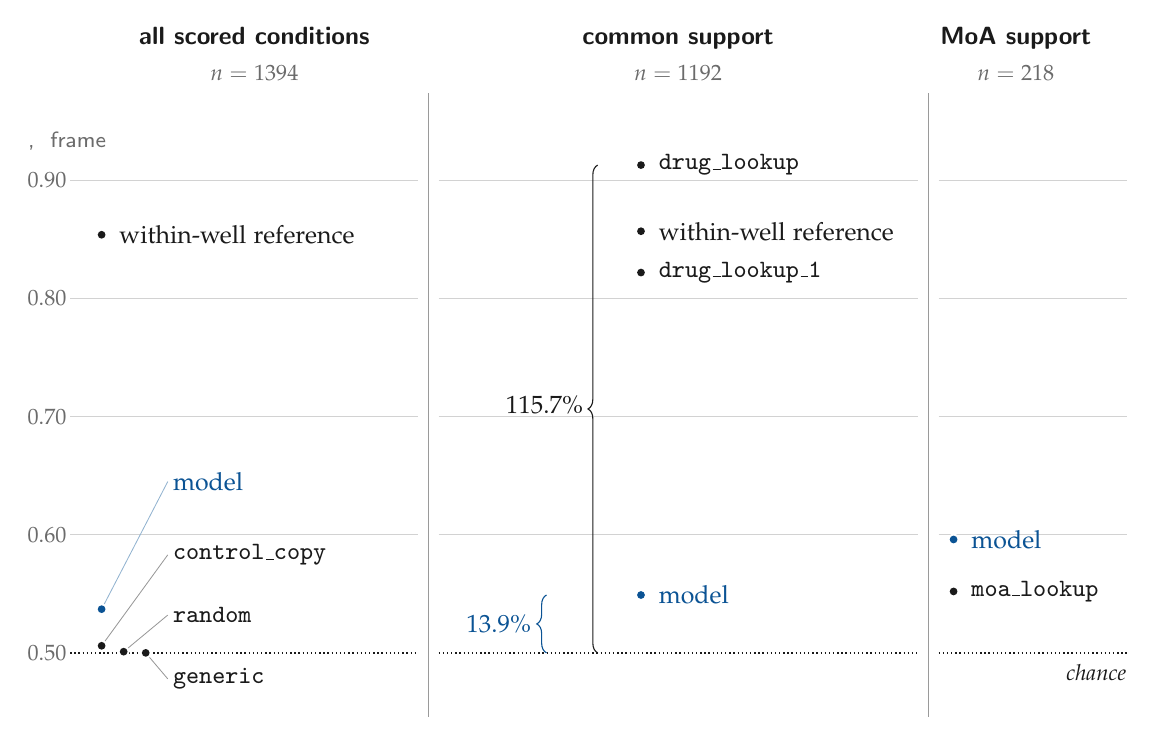
\begin{tikzpicture}[x=1cm, y=72mm, every node/.style={inner sep=0pt}]

  % --- value-to-position map. One map, one axis, all three columns. ---------
  \def\lo{0.47}\def\hi{0.95}
  \def\Y#1{{(#1-\lo)/(\hi-\lo)}}

  % --- the three registers of label type, and the furniture sizes. ---------
  % 9pt, not \scriptsize (8pt): this figure is drawn at its final size and is
  % never scaled, so its type may sit just under the 11pt caption rather than
  % being shrunk below it.
  \def\marklab{\fontsize{9}{10.5}\selectfont}
  \def\ticklab{\fontsize{8}{9}\selectfont}
  \def\headlab{\sffamily\fontsize{9}{10.5}\selectfont\bfseries}
  \def\subhead{\sffamily\fontsize{8}{9.5}\selectfont}

  % --- column geometry (cm): the two dividers and the right edge. ----------
  \def\Da{4.45}\def\Db{10.80}\def\R{13.32}

  % --- drawing macros. Order of use is leaders, then dots, then labels, so a
  %     dot and its halo always cover the tail of its own leader. -----------
  \newcommand{\lead}[5]{\draw[#5!45, line width=0.3pt]
     (#1,\Y{#2}) -- (#3-0.06,\Y{#4});}
  \newcommand{\dotat}[3]{\fill[white] (#1,\Y{#2}) circle (2.1pt);
     \fill[#3] (#1,\Y{#2}) circle (1.4pt);}
  \newcommand{\labat}[4]{\node[anchor=west, text=#3, font=\marklab]
     at (#1,\Y{#2}) {#4};}

  % --- gridlines, broken at the dividers ------------------------------------
  \foreach \v in {0.60,0.70,0.80,0.90}{
    \draw[rulegrey!45, line width=0.3pt] (-0.10,\Y{\v}) -- (4.32,\Y{\v});
    \draw[rulegrey!45, line width=0.3pt] ( 4.58,\Y{\v}) -- (10.67,\Y{\v});
    \draw[rulegrey!45, line width=0.3pt] (10.93,\Y{\v}) -- (\R,\Y{\v});}
  \foreach \v in {0.50,0.60,0.70,0.80,0.90}{
    \node[anchor=east, font=\ticklab, text=quietink] at (-0.14,\Y{\v}) {\v};}

  % --- the chance rule. Drawn, and named, because the axis is NIR. ----------
  \draw[ink, line width=0.5pt, densely dotted] (-0.10,\Y{0.50}) -- (4.32,\Y{0.50});
  \draw[ink, line width=0.5pt, densely dotted] ( 4.58,\Y{0.50}) -- (10.67,\Y{0.50});
  \draw[ink, line width=0.5pt, densely dotted] (10.93,\Y{0.50}) -- (\R,\Y{0.50});
  \node[anchor=east, font=\ticklab\itshape, text=ink] at (\R,\Y{0.483}) {chance};

  % --- what the axis is -----------------------------------------------------
  \node[anchor=west, font=\subhead, text=quietink]
    at (-0.64,\Y{0.933}) {$\NIR$, \Rframe{} frame};

  % --- column dividers and column heads -------------------------------------
  \draw[rulegrey, line width=0.4pt] (\Da,-0.05) -- (\Da,1.05);
  \draw[rulegrey, line width=0.4pt] (\Db,-0.05) -- (\Db,1.05);
  \node[anchor=south, align=center, text=ink] at (2.24,1.07)
    {{\headlab all scored conditions}\\[0.2ex]{\subhead\color{quietink}$n = \num{1394}$}};
  \node[anchor=south, align=center, text=ink] at (7.62,1.07)
    {{\headlab common support}\\[0.2ex]{\subhead\color{quietink}$n = \num{1192}$}};
  \node[anchor=south, align=center, text=ink] at (11.91,1.07)
    {{\headlab MoA support}\\[0.2ex]{\subhead\color{quietink}$n = \num{218}$}};

  % =========================================================================
  % COLUMN 1 -- all scored conditions, n = 1394
  % =========================================================================
  % Four fanned leaders. Dots are dodged sideways only where values coincide:
  % control_copy 0.506, random 0.501, generic 0.500 are 0.8mm and 0.16mm apart
  % vertically here, against a 1.0mm dot.
  \lead{0.30}{0.537}{1.20}{0.645}{accent}
  \lead{0.30}{0.506}{1.20}{0.583}{ink}
  \lead{0.58}{0.501}{1.20}{0.532}{ink}
  \lead{0.86}{0.500}{1.20}{0.478}{ink}

  \dotat{0.30}{0.854}{ink}
  \dotat{0.30}{0.537}{accent}
  \dotat{0.30}{0.506}{ink}
  \dotat{0.58}{0.501}{ink}
  \dotat{0.86}{0.500}{ink}

  \labat{0.52}{0.854}{ink}{within-well reference}
  \labat{1.20}{0.645}{accent}{model}
  \labat{1.20}{0.583}{ink}{\ttfamily control\_copy}
  \labat{1.20}{0.532}{ink}{\ttfamily random}
  \labat{1.20}{0.478}{ink}{\ttfamily generic}

  % =========================================================================
  % COLUMN 2 -- common support of the drug lookups, n = 1192
  % =========================================================================
  % Coverage of the reference, (arm - 0.50) / (reference - 0.50), both on THIS
  % support. Braces first so the dots' halos are not cut by a brace stem.
  \draw[decorate, decoration={brace, amplitude=3.5pt}, accent, line width=0.4pt]
    (5.95,\Y{0.500}) -- (5.95,\Y{0.549});
  \node[anchor=east, font=\marklab, text=accent] at (5.76,\Y{0.5245}) {$13.9\%$};
  \draw[decorate, decoration={brace, amplitude=3.5pt}, ink, line width=0.4pt]
    (6.60,\Y{0.500}) -- (6.60,\Y{0.913});
  \node[anchor=east, font=\marklab, text=ink] at (6.42,\Y{0.710}) {$115.7\%$};

  \dotat{7.15}{0.913}{ink}
  \dotat{7.15}{0.857}{ink}
  \dotat{7.15}{0.822}{ink}
  \dotat{7.15}{0.549}{accent}

  \labat{7.37}{0.913}{ink}{\ttfamily drug\_lookup}
  \labat{7.37}{0.857}{ink}{within-well reference}
  \labat{7.37}{0.822}{ink}{\ttfamily drug\_lookup\_1}
  \labat{7.37}{0.549}{accent}{model}

  % =========================================================================
  % COLUMN 3 -- conditions with an MoA partner pool, n = 218
  % =========================================================================
  \dotat{11.12}{0.596}{accent}
  \dotat{11.12}{0.552}{ink}

  \labat{11.34}{0.596}{accent}{model}
  \labat{11.34}{0.552}{ink}{\ttfamily moa\_lookup}

\end{tikzpicture}

\caption[The baseline ladder]{\textbf{A predictor that needs no model, no prompt
and no checkpoint scores above the reference the model is measured against, and
the three columns may not be read across.} Marks are $\NIR$ in the \Rframe{}
frame, where chance is $0.50$. Each column is scored on its own support
($n = \num{1394}$, $\num{1192}$ and $\num{218}$), so a mark in one may not be set
beside a mark in another; even the reference differs between the first two. On
the common support the model covers $13.9\%$ of the distance from chance to the
within-well split-half precision reference, and a training-only per-drug lookup
covers $115.7\%$ of it, which is a property of the reference and not headroom
(\cref{tab:lookup}). On the MoA support the model scores $0.596$ against
\texttt{moa\_lookup}'s $0.552$, a $+0.0436$ the interval does not separate from
zero. No interval is drawn: the source gives them on differences between arms,
not on the level of one arm, and those are in \cref{tab:lookup}. \emph{Reading
the labels}: monospace names an arm exactly as \cref{tab:lookup} names it, roman
names the reference in prose, the accent marks the model, and there is no fourth
style. A label a rule would strike or a neighbour would crowd is lifted clear on
a hairline; the dot carries the value. Horizontal position inside a column means
nothing, and arms whose scores nearly coincide are dodged sideways so each keeps
its own dot.}
\label{fig:ladder}
\end{figure}

% ---------------------------------------------------------------------------
\begin{table}[htbp]
\begin{fullwidth}
\begin{threeparttable}
\caption{\textbf{A training-only per-drug lookup is the bar to beat.} Reference,
model and drug-agnostic arms use all $\num{1394}$ conditions; the drug lookups
exist on a common support of $\num{1192}$, where model and reference score
$0.549$ and $0.857$. There, model minus \texttt{drug\_lookup} is
\ci{-0.3631}{-0.3982}{-0.3280}; the lookup scores $0.913$ pooled, $0.980$ on
trained conditions and $0.890$ on held-out wells, where its same-well advantage
is absent. \texttt{moa\_lookup} has narrower support ($n = \num{218}$) and is not
separated from the model (\ci{+0.0436}{-0.0480}{+0.1352}); its pooled row must
not be compared with rows on other supports.}
\label{tab:lookup}
\small
\begin{tabularx}{\linewidth}{@{}%
  >{\raggedright\arraybackslash}p{0.28\linewidth}
  >{\raggedright\arraybackslash}p{0.22\linewidth}
  S[table-format=1.3]
  >{\raggedright\arraybackslash}X@{}}
\toprule
\thead{Arm} & \thead{What it knows} & {\thead{$\NIR$}} & \thead{Note} \\
\midrule
within-well split-half reference & disjoint cell halves, one well & 0.854
  & precision, not a replicate; $0.857$ on the lookups' support \\
\addlinespace
\texttt{drug\_lookup} (training-only) & drug's mean residual, other lines & 0.913
  & the bar to beat; $n = \num{1192}$ \\
\texttt{drug\_lookup\_1} & the same, from one other cell line & 0.822
  & still beats the model; same support \\
\texttt{moa\_lookup} ($n = \num{218}$) & drugs sharing this drug's MoA & 0.552
  & narrower support; not separated \\
\addlinespace
model & control cell $+$ drug & 0.537
  & $0.549$ on the lookups' $n = \num{1192}$ \\
\addlinespace
\texttt{control\_copy} & nothing (copies the control) & 0.506 & drug-agnostic \\
\texttt{generic} & nothing (predicts the average) & 0.500 & the zero vector \\
\texttt{random} & nothing & 0.501 & floor \\
\bottomrule
\end{tabularx}
\begin{tablenotes}[flushleft]\footnotesize
\item Rows on different supports are not comparable. Chance is $0.50$ in the
\Rframe{} frame under the exchangeability condition audited in
\cref{sec:res-metrics}.
\end{tablenotes}
\end{threeparttable}
\end{fullwidth}
\end{table}

% ---------------------------------------------------------------------------
\paragraph{The pre-registered middle branch fired} Of the three branches written
before the result, the middle one fired. The model reads the drug and recovers
only a small fraction of its residual; transfer to held-out combinations is
\notestablished (\cref{sec:res-generalisation}). Whether its sensitivity to the
prompt reduces to the \texttt{Mechanism:} field is not settled here. On the
$\num{218}$ conditions where that comparison exists, model $-$
\texttt{moa\_lookup} $=
\ci{+0.0436}{-0.0480}{+0.1352}$, clustered on cell line and well, an interval
spanning zero.

\paragraph{This is DrEval's finding, in transcriptomic space} The finding travels
furthest of anything here, needing no checkpoint, no prompt and no cell-sentence
encoding. DrEval reports that deep learning models barely outperform a naive
predictor of mean drug and cell-line effects~\cite{dreval}, and our
\texttt{drug\_lookup} is
the $\beta(d)$ term of that additive model, measured where the
$\textrm{generic}(c)$ term has already been
subtracted.\seealso{\cref{sec:res-transfer} measures what that constant leaves
out} On a $946$-gene transcriptomic response, not a scalar potency, that drug
main effect reaches $0.913$, above the $0.857$ reference itself. DrEval's
inherited warning~\cite{partin}, that good pair-holdout performance is reachable
by predicting each drug's training average, is here the hypothesis. It holds.

\paragraph{The missing head-to-head, and why the bar survives it} A third
objection is that this chapter's model is the wrong one. A conditional model
built for perturbation response~\cite{cpa,scgen,gears} was never run on this
split, so the head-to-head a reader wants is missing, and that is a real gap. But
the ladder is architecture-free, so a competitor can be dropped in and scored,
and what it has to clear for a seen drug in a new context is
\texttt{drug\_lookup}, $0.913$ pooled, or $0.890$ on the held-out split. Not
$0.500$. For an unseen drug no lookup exists, so that regime needs a different
bar and gets one in \cref{sec:res-scope}.

\begin{scopelimit}[carried into \cref{sec:res-scope} and \cref{sec:limitations}]
The two regimes must not share a number. \texttt{drug\_lookup} is the bar for a
\emph{seen} drug in a new context. No lookup exists for a drug that never
appeared in training, so nothing here sets a bar for that regime. Neither may
rows on different supports be combined: $\num{1394}$, $\num{1192}$ and
$\num{218}$ select conditions by different rules, and a distance to the reference
is comparable within a support and not between supports.
\end{scopelimit}

\paragraph{Why the lookup beating the reference is not headroom} On the common
support the lookup scores \emph{above} the reference,
$\texttt{drug\_lookup} - \textrm{reference} = +0.056$, tempting to read as ``the
modelling target has vanished''. Three reasons, all favouring the lookup, block
that inference. The reference is scored against a half-sample truth and every
baseline against the full-sample truth; \texttt{drug\_lookup} averages
$\approx 38$ conditions against that single noisy half; and $\NIR$ near $0.91$
compresses most of the cosine range into a few thousandths. The coverage figures
are themselves distances to a split-half reference \cref{sec:methods-data} calls
optimistic; that optimism sits in the denominator and if anything makes both
coverage figures too small, while the half-sample truth of the first reason
pushes the other way. The net magnitude is unknown and the ordering carries the
claim.

\paragraph{Averaging is not why the lookup beats the model} Of those three
reasons only the averaging could also deflate the comparison with the model, and
\texttt{drug\_lookup\_1} tests it by drawing on one other cell line. It scores
$0.822$, and paired on the same support the model trails it by
\ci{-0.2723}{-0.3074}{-0.2372}, clustered two-way on cell line and well. This
drug's mean residual in one other cell line beats a $1$B-parameter model handed
this condition's own control cells. Neither gap is an average over a mixed
population (\cref{fig:paired-lookup}): condition by condition, the model scores
above \texttt{drug\_lookup} on $85$ of the $\num{1192}$ and above
\texttt{drug\_lookup\_1} on $214$, $7.1\%$ and $18.0\%$, counts over conditions
carrying no interval.

\paragraph{The bar is not equally clean on both sides of the split} The pooled
$0.913$ covers two populations. On trained conditions the lookup scores $0.980$.
On held-out wells, where it cannot borrow the target's own well, it scores
$0.890$ against the model's $0.533$ on the \needsaudit{893} held-out-well
conditions where both are scored, a count this thesis quotes two ways and has
under audit; the paired gap there is \ci{-0.357}{-0.403}{-0.311}. Nothing in the
argument turns on the exact size of that population. The ordering holds on both
sides, and the held-out side, where the well advantage is absent, is the side a
claim about transfer has to survive.

% ---------------------------------------------------------------------------
% \begin{fullwidth}: two square scatters side by side, each with its own
% difference histogram beneath, is a 174mm object -- squeezed to the 142mm body
% block the two panels lose the aspect that makes the identity line readable as
% a diagonal. Drawn at 174mm by thesis_v2/figs/paired-lookup.py, so NO width=
% key: it is placed at scale 1.0 and its type prints at the size it was set in.
% Every number it draws is listed with its source pointer in
% figs/fig-paired-lookup.json.
\begin{figure}[htbp]
\begin{fullwidth}
\centering
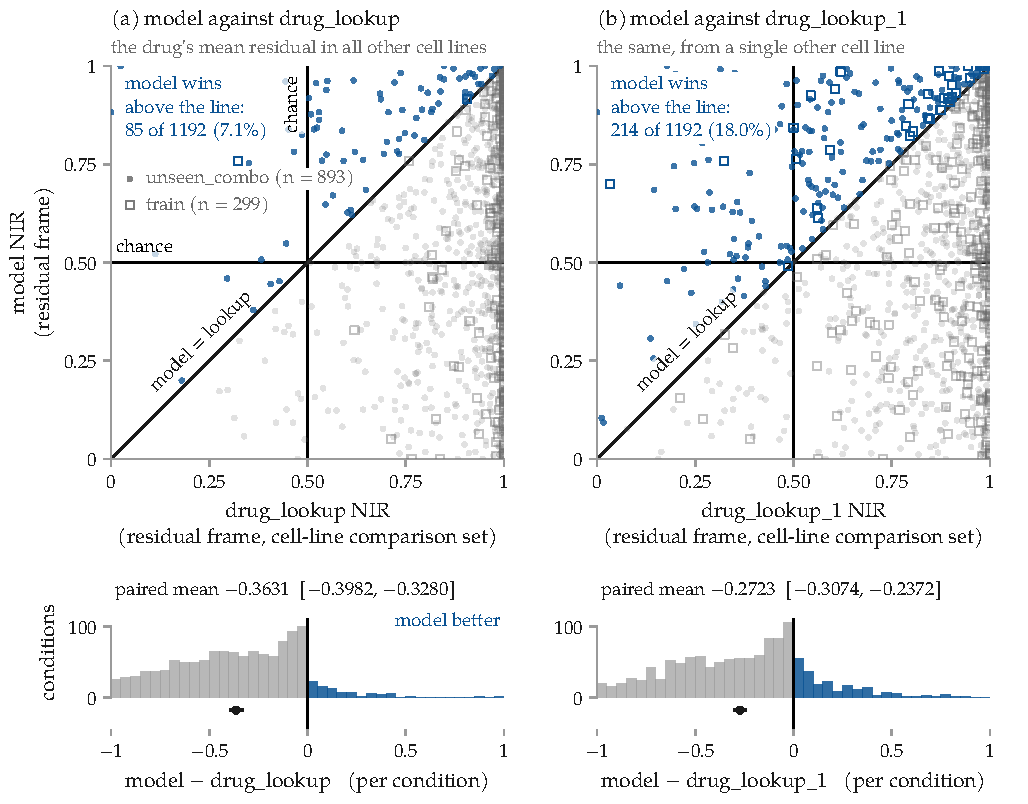
\includegraphics{fig-paired-lookup}
\caption[The model beats the lookup on 7.1\% of conditions]{\textbf{The headline
gap is a tilt of nearly the whole population and not a mean over a mixed one:
the model scores above \texttt{drug\_lookup} on $7.1\%$ of conditions, and above
the single-cell-line lookup on $18.0\%$.} Every mark is one of the $\num{1192}$
conditions of the common support --- those on which a training-only lookup
exists --- and both axes are $\NIR$ in the \Rframe{} frame, comparison set other
drugs in the same cell line. On this support the model scores $0.549$ and the
within-well split-half precision reference $0.857$; the $\num{1394}$-condition
figures quoted elsewhere ($0.537$ and $0.854$) are a different population and
are not combined with these. \textbf{(a)}~Against \texttt{drug\_lookup}, the
drug's mean residual in all other cell lines, $0.913$ pooled: the model is above
the identity line on $85$ of $\num{1192}$ conditions, $7.1\%$.
\textbf{(b)}~Against \texttt{drug\_lookup\_1}, the same quantity from a single
other cell line, $0.822$ pooled: $214$ of $\num{1192}$, $18.0\%$. Marker shape
gives the split, $\num{299}$ \texttt{train} and \needsaudit{893}
\texttt{unseen\_combo}; no \texttt{unseen\_drug} condition appears, because no
training lookup exists for a drug held out of training, and that regime is
therefore not addressed by this figure at all. The lower panels are the
per-condition paired difference on a shared count axis, with the paired mean
drawn below the counts as a point and bar, the bar a $95\%$ bootstrap interval
clustered two-way on cell line and well: \ci{-0.3631}{-0.3982}{-0.3280} in (a)
and \ci{-0.2723}{-0.3074}{-0.2372} in (b). The win counts are counts over
conditions and carry no interval; ties ($23$ and $28$ conditions) count as not a
win. The $0.50$ rules are chance on both axes, labelled once in (a).}
\label{fig:paired-lookup}
\end{fullwidth}
\end{figure}

\begin{claim}
The honest summary is the paired gap on common support ($n = \num{1192}$),
\ci{-0.3631}{-0.3982}{-0.3280}. The model covers $13.9\%$ of the distance from
chance to the within-well split-half precision reference where a training-only
lookup covers all of it and more. Those are common-support figures, model $0.549$
against reference $0.857$; over all $\num{1394}$ scored conditions, not all of
which admit a lookup, the model is $0.537$ against a reference of $0.854$, and
the two populations are not combined. The pooled gap does combine the two sides
of the split, on which the lookup is not equally clean. On held-out conditions
alone it is \ci{-0.357}{-0.403}{-0.311}, and the lookup's $0.913$ is $0.980$ on
trained conditions against $0.890$ on held-out ones. That the lookup exceeds the
reference is a property of the reference, not a headroom estimate; the reference
is a single noisy half-sample while the lookup averages many cell lines, and
$\NIR$ compresses near its top. Nor is averaging what beats the model. Restricted
to a \emph{single} other cell line the lookup scores $0.822$ and the model still
trails it by \ci{-0.2723}{-0.3074}{-0.2372}. This is DrEval's finding replicated
in transcriptomic space, the drug main effect at $0.913$ where a $1$B-parameter
model reaches $0.549$. Being a bar and not a result is what makes it reusable,
and any method proposed for seen-drug transfer on this atlas has to clear it, not
merely chance.
\end{claim}

% ===========================================================================
\beatsection{R}{8}{Same-target retrieval is the strongest observed lead}{sec:res-scope}
\claimlede{Same-target retrieval is the strongest observed lead on its own
restricted support; because the three channel arms differ in support, drug
roster, partner count and annotation coverage, that is a descriptive result and
not an identified biological ranking.}

\begin{question}[8]
The bar just set exists only for a drug that appeared in training. A drug that
never did can be reached at all only through some property it shares with drugs
that were seen, a protein target, a mechanism, a chemical shape. The instrument
predicts each drug from its annotated neighbours in the same cell line, against a
null matched on everything but the channel itself. One channel carries a lead, on
a very short roster of drugs.
\end{question}

\noindent
For a channel $X$, a drug's residual is predicted as the mean residual of the
other drugs in the same cell line sharing property $X$ with it, the construction
of \texttt{moa\_lookup} (\cref{sec:res-lookup}) generalised from mechanism to any
annotated property.

\paragraph{The null has to differ in exactly one respect} The gate's estimand
requires the channel arm and its null to differ in the channel and in nothing
else. Every channel is paired with a plate-matched random null carrying the same
number of partner drugs, drawn from the same cell line, with the same split
across the target's own plate and other plates. Mechanism- and target-related
drugs are co-plated more often than chance, so a null matched on count alone
would differ in plate membership too, two differences where the estimand allows
one. Where a plate-matched null spans too few cell lines the channel is reported
\textsc{untestable}. ``We could not build the control'' must never be written as
``closed''. Coverage is printed first as well, because a channel annotated on few
drugs was never really tested and cannot be closed by a null result.

\paragraph{The partner pool was wrong, and every verdict here is from the re-run}
The gate was intended to draw partners only from drugs that were in training,
which is what makes it a fair contest in every split. An audit of its own
implementation, not of the already-restricted lookup arms of
\cref{sec:res-lookup}, found the pool spanning every retained condition in the
cell line. The restriction is now in the code. Of the
\needsaudit[what retained counts]{4{,}131} retained conditions only
\needsaudit{$\num{2523}$} are training, so nearly two in five the old pool could
draw on were ineligible.
Every verdict here is from the corrected run, which moved the target gap down,
the mechanism gap up, and chemistry's down by half.\corrmark{the channel gate's
partner pool, restricted and re-run}

% ---------------------------------------------------------------------------
\begin{table}[htbp]
\begin{fullwidth}
\begin{threeparttable}
\caption{\textbf{Coverage first, then the gap.} The drugs behind each channel are
stated before any verdict, because a null result on a channel never really tested
is not a closure. The plate-matched null is the estimand-correct control; the
count-matched column shows sensitivity to plate membership, not a causal share.
The gate asks the plate-matched lower bound to clear a pre-set margin of $0.03$
clustered on cell line and well. On that axis, and only there, protein target
clears it ($+0.0745$) while mechanism ($+0.0279$) and chemistry ($+0.0035$) do
not. All three exclude zero, so the two that fail are inconclusive rather than
equivalent to their nulls, and neither may be written as closed.}
\label{tab:channels}
\small
\begin{tabularx}{\linewidth}{@{}%
  >{\raggedright\arraybackslash}p{0.15\linewidth}
  >{\centering\arraybackslash}p{0.13\linewidth}
  >{\centering\arraybackslash}p{0.06\linewidth}
  >{\centering\arraybackslash}p{0.23\linewidth}
  >{\centering\arraybackslash}p{0.11\linewidth}
  >{\raggedright\arraybackslash}X@{}}
\toprule
\thead{Channel} & \thead{Drugs (annot./scored)} & \thead{$n$}
  & \thead{vs plate-matched null} & \thead{(vs count-matched)}
  & \thead{Verdict} \\
\midrule
\textbf{protein target} & 264 / 18 & 712 & \ci{+0.1351}{+0.0745}{+0.1958}
  & $+0.1498$ & live, cell-line axis$^{\dagger}$ \\
\addlinespace
mechanism (MoA) & 180 / 26 & 921 & \ci{+0.0805}{+0.0279}{+0.1332}
  & $+0.0623$ & inconclusive \\
\addlinespace
chemical structure & 377 / 94 & \needsaudit{4131}
  & \ci{+0.0261}{+0.0035}{+0.0487} & $+0.0122$ & inconclusive \\
\bottomrule
\end{tabularx}
\begin{tablenotes}[flushleft]\footnotesize
\item $^{\dagger}$The axis is written into the target verdict because ``live'' is
not usable without it. Clustered on the drug, the target interval falls short of
this margin against both estimand-correct nulls and clears it only against the
weaker count-matched one.
\item The counts are annotations in Tahoe's drug metadata and not testable
coverage here; within this cache only $18$, $26$ and $94$ of the $94$ scored
drugs received a channel arm at all.
\end{tablenotes}
\end{threeparttable}
\end{fullwidth}
\end{table}

% ---------------------------------------------------------------------------
% \input, not \includegraphics: figs/gate.tex is TikZ and carries its own float,
% fullwidth block, caption and \label{fig:gate}. Its twelve intervals are
% literals transcribed from RESULTS_cluster/ and listed again, to machine
% precision and with their n, cluster keys, df and source paths, in the sibling
% figs/fig-gate.json.
% ===========================================================================
% gate.tex -- the channel gate, twelve intervals in three blocks.
% \input by Sections/04d-baselines.tex, replacing the inline tikzpicture that
% sat at lines 391-455 there. Compiles against thesis_v2/preamble.tex and
% nothing else. NO external data at draw time: every coordinate below is a
% literal transcribed from RESULTS_cluster/ and listed again, to full machine
% precision and with its n and cluster keys, in the sibling figs/fig-gate.json.
%
% SOURCES, one per block. Nothing here is computed in the figure.
%   block 1  RESULTS_cluster/channel_gate_v4.json
%            channels.<ch>.{plate_matched,different_plate}.{gap,ci}
%            ci is the two-way cell-line x well interval (df 38 / 40 / 41).
%   block 2  RESULTS_cluster/channel_gate_v4_byaxis.json
%            channels.target.<null>.ci_drug_well (df 17); the gap is the same
%            number as in block 1 -- re-clustering moves the interval only.
%   block 3  RESULTS_cluster/channel_gate_heldout_targets.json
%            channels.<ch>.heldout_targets.{gap,ci}, cell line x well again
%            (df 4 / 10 / 39).
% Each row's n is the .n at that same path, transcribed with it; block 2 re-uses
% block 1's records, so its counts are block 1's and only the clustering differs.
% Every drawn value equals the four-decimal figure the prose and tab:channels
% already print; the agreement was checked value by value, in both directions,
% against 04d-baselines.tex lines 350-354, 369-376, 470-479, 521-526 and 684.
%
% WHAT CHANGED FROM THE VERSION IT REPLACES, and why. The old drawing was sound
% -- greyscale-safe, no chartjunk, blocks separated, caption forbidding a read
% across blocks -- and five things were wrong with it, the fifth found in a
% review of this file's own first version:
%
%   1. THE AXIS HAD NO NAME. It carried ticks, a dotted line and a dashed line
%      and nowhere said what was being measured, so a reader could not tell an
%      NIR gap from a DRF or a coverage without going back to tab:channels one
%      page earlier. There is now an axis title over the data area naming the
%      quantity (a gap in NIR), its direction (arm minus matched null), its
%      scale (NIR runs 0 to 1, chance 0.50) and what zero means. This is the
%      one thing the figure genuinely needed. It ran to two lines as first
%      written; the third, naming the frame, is fix 5 below.
%
%   2. THE ORIGIN WAS LABELLED IN WORDS while the other ticks were numerals --
%      "zero" beside 0.10 and 0.20 on one axis. The origin is now 0.00, in the
%      same face, size and colour as its neighbours, on the dotted rule.
%
%   3. THE TWO CALLOUTS SAT ON TOP OF EACH OTHER. "zero" and "margin" labelled
%      two rules 5.5mm apart, in two different styles, at the same height. The
%      zero rule now carries a numeral in the tick row; the margin keeps a
%      worded callout, raised so the gap between the two label boxes is
%      0.82 y-units = 4.4mm of clear space (y=5.4mm; inner sep is pinned at
%      1pt below so this is box arithmetic, not judgement, and the ink gap is
%      wider still). The dashed rule is carried up to meet its own callout, so
%      no separate leader is needed.
%
%   4. THE AXIS STOPPED AT ZERO but two rows did not. mechanism-on-four runs to
%      -0.0846 and chemistry-different-plate to -0.0097, so rows extended into
%      a region with no tick and no label. The tick set now runs
%      -0.10, 0.00, 0.10, 0.20 at a uniform 0.10 pitch and the negative region
%      the third block occupies is labelled like any other.
%
%   5. THE AXIS NAMED THE QUANTITY BUT NOT THE FRAME, and no row carried its
%      own n. Fix 1 said what was measured, a gap in NIR, and left out where it
%      was measured. This document runs two measurement frames that both put
%      chance at 0.50, and conflating them is its most common misread -- the
%      running head exists for that reason alone -- so an NIR figure naming
%      neither the frame nor the set the score is ranked against is
%      under-labelled in exactly the way fix 1 was, one level up. A third title
%      line now names both, in the wording 04d-baselines.tex uses at 714-716
%      and fig:comparator uses in its caption: the residual frame, scored
%      against the other drugs in the same cell line. The caption says it too,
%      so the figure does not depend on the running head to carry its frame.
%      Twelve rows also carried no counts while tab:channels, one page earlier,
%      carries three; each row now prints its own n in a column of its own,
%      headed n, so what a block rests on is visible where the block is. The
%      three plate-matched counts in block 1 are tab:channels' n column, value
%      for value; the chemistry count keeps that table's audit flag, since a
%      quantity flagged in one place and printed clean in another is exactly
%      the divergence the flag exists to prevent. Every count is in
%      fig-gate.json, per row, with its source path.
%
% GEOMETRY, all of it derived rather than judged. x=108mm is the DATA area,
% spanning \alo..\ahi = -0.115..0.265, so 0.10 of NIR is 28.4mm.
%   padding    set by the data: leftmost ink is the -0.0846 whisker cap, 8.7mm
%              clear of the left edge; rightmost the +0.2460 cap, 5.7mm clear
%              of the right.
%   labels     column 60.0mm = 0.5556 x-units, set by the longest string in it,
%              the block head "targets restricted to drugs held out of
%              training" at 166.38pt = 58.5mm (measured, figs/
%              _measure_gate_strings.tex). Nothing in the column reaches the
%              data area, so no label can foul the -0.10 rule, which stands
%              4.3mm inside the left edge. Longest ROW label is 42.2mm.
%   counts     the n column is right-aligned inside that same 60.0mm, its right
%              edge 1.5mm clear of the data area and therefore 5.8mm clear of
%              the -0.10 rule. Its widest entry is the audit-flagged 4,131 chip
%              at 24.60pt = 8.65mm, and that entry sits on the row carrying the
%              longest label, "chemical structure, plate-matched" at 120.04pt =
%              42.19mm; label and count are 6.96mm apart with the 1pt inner sep
%              counted at both ends, which is the tightest pair in the column.
%              The column takes space the label column already had, so the
%              drawing does not widen: the harness reports the same 484.15pt
%              before and after.
%   rules      block separators start 1mm left of the label column and end at
%              the right edge of the data area.
%   width      1.5648 x-units = 169.0mm against the 174mm a fullwidth float may
%              use; 5mm of slack. MEASURED by figs/_harness_gate.tex, which
%              \typeout s \wd of the tikzpicture against the real preamble.
%   title      all three lines fit inside the 108mm data area they are centred
%              on (78.76mm, 88.08mm and 102.13mm measured), so none widens the
%              drawing. The block sits 0.65 y-units = 3.51mm higher than it did
%              to make room for the frame line; height is the only dimension
%              this change moves, and the float is nowhere near \topfraction.
%
% TYPE. \scriptsize throughout, matching fig:clustering and fig:confound. This
% drawing is not scaled by anything, so 8pt here prints as 8pt.
% ===========================================================================
\begin{figure}[htbp]
\begin{fullwidth}
\centering
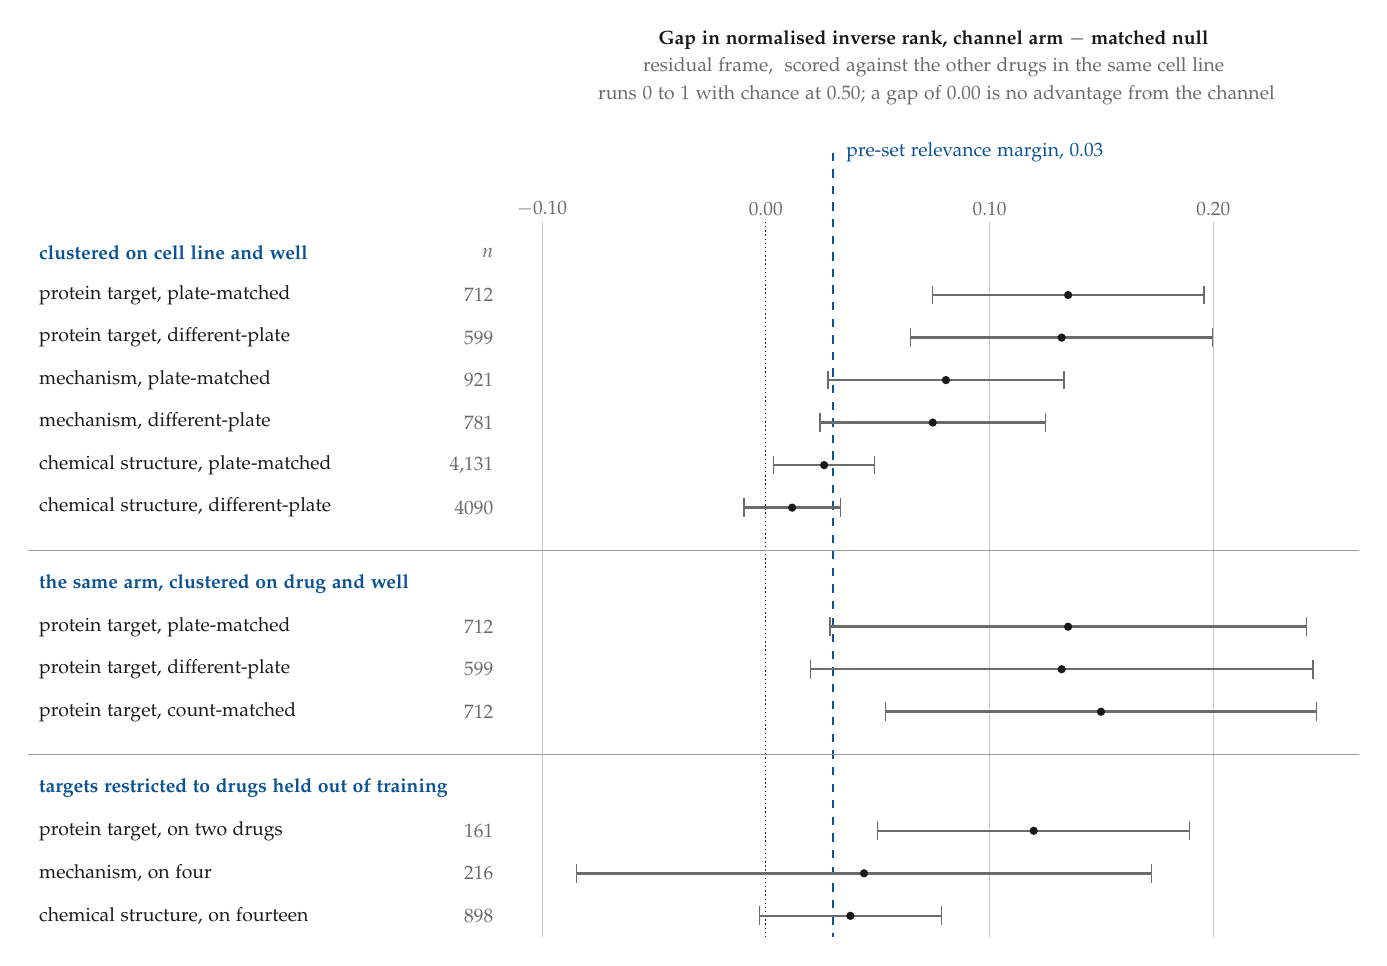
\begin{tikzpicture}[x=108mm, y=5.4mm, font=\small, inner sep=1pt]
  \def\alo{-0.115}\def\ahi{0.265}  % data range of the x axis
  \def\lx{-0.5556}                 % left edge of the row-label column (60.0mm)
  \def\rx{-0.5648}                 % left end of the block rules      (61.0mm)
  \def\ytop{0.72}                  % top of the tick rules and the zero rule
  \def\ybot{-16.1}                 % bottom of the same
  \def\cx{-1.5mm}                  % right edge of the n column, from x=0
  \newcommand{\vx}[1]{{(#1-\alo)/(\ahi-\alo)}}

  % --- one interval row: #1 y, #2 lo, #3 estimate, #4 hi, #5 label, #6 n ---
  % FIX 5: #6 is the row's own count, right-aligned against \cx. A column, not a
  % caption list: twelve counts in prose cannot be matched to twelve rows by eye,
  % and this is how tab:channels carries them one page earlier.
  \newcommand{\gaprow}[6]{%
    \draw[quietink, line width=0.9pt] (\vx{#2},#1) -- (\vx{#4},#1);
    \draw[quietink, line width=0.5pt]
      (\vx{#2},#1-0.22) -- (\vx{#2},#1+0.22);
    \draw[quietink, line width=0.5pt]
      (\vx{#4},#1-0.22) -- (\vx{#4},#1+0.22);
    \fill[ink] (\vx{#3},#1) circle (1.5pt);
    \node[anchor=west, font=\scriptsize, text=ink] at (\lx,#1) {#5};
    \node[anchor=east, font=\scriptsize, text=quietink, xshift=\cx]
      at (0,#1) {#6};}
  \newcommand{\blockhead}[2]{%
    \node[anchor=west, font=\scriptsize\bfseries, text=accent]
      at (\lx,#1) {#2};}

  % --- FIX 1: the axis title. What is measured, in which direction, on what
  % scale, and what zero means. Centred on the data area, not on the drawing.
  % FIX 5 adds the middle line: in which frame, and against which set the score
  % is ranked. Both frames in this document put chance at 0.50, so the scale
  % line below does not distinguish them and cannot be left to do that work.
  \node[anchor=south, font=\scriptsize\bfseries, text=ink] at (0.5,4.70)
    {Gap in normalised inverse rank, channel arm $-$ matched null};
  \node[anchor=south, font=\scriptsize, text=quietink] at (0.5,4.05)
    {residual frame, $\NIR$ scored against the other drugs in the same
     cell line};
  \node[anchor=south, font=\scriptsize, text=quietink] at (0.5,3.40)
    {$\NIR$ runs $0$ to $1$ with chance at $0.50$; a gap of $0.00$
     is no advantage from the channel};

  % --- the scale. FIX 4: the tick set now covers the negative region. ------
  \foreach \v/\t in {-0.10/$-0.10$, 0.10/0.10, 0.20/0.20}{
    \draw[rulegrey!55, line width=0.3pt] (\vx{\v},\ytop) -- (\vx{\v},\ybot);
    \node[anchor=south, font=\scriptsize, text=quietink]
      at (\vx{\v},\ytop+0.06) {\t};}

  % zero, and FIX 2: a numeral, in the same row and register as the others.
  \draw[ink, line width=0.5pt, densely dotted] (\vx{0},\ytop) -- (\vx{0},\ybot);
  \node[anchor=south, font=\scriptsize, text=quietink]
    at (\vx{0},\ytop+0.06) {0.00};

  % the pre-set relevance margin. FIX 3: the rule is carried up to its own
  % callout, 4.4mm of clear space above the tick numerals.
  \draw[accent, line width=0.6pt, dashed] (\vx{0.03},2.35) -- (\vx{0.03},\ybot);
  % (the 1.3mm stand-off is an xshift, not an addition to \vx: \vx expands to
  % a braced pgfmath group and "{...}+0.012" is not a legal coordinate.)
  \node[anchor=west, font=\scriptsize, text=accent, xshift=1.3mm]
    at (\vx{0.03},2.35) {pre-set relevance margin, $0.03$};

  % --- block 1: cell line x well, the axis the gate was run on -------------
  % The n column is headed once, on the first block head's own row: that head is
  % 38.4mm of the 60.0mm column and stops 11mm short of the column, so the two
  % cannot touch. Blocks 2 and 3 keep the same column position and the caption
  % names it, so the head is not repeated over rules it would be read across.
  \blockhead{0}{clustered on cell line and well}
  \node[anchor=east, font=\scriptsize, text=quietink, xshift=\cx] at (0,0) {$n$};
  \gaprow{-1}{+0.0745}{+0.1351}{+0.1958}{protein target, plate-matched}{\num{712}}
  \gaprow{-2}{+0.0648}{+0.1322}{+0.1996}{protein target, different-plate}{\num{599}}
  \gaprow{-3}{+0.0279}{+0.0805}{+0.1332}{mechanism, plate-matched}{\num{921}}
  \gaprow{-4}{+0.0243}{+0.0746}{+0.1249}{mechanism, different-plate}{\num{781}}
  % the flagged count is tab:channels' own \needsaudit{4131}, carried here so the
  % same quantity is not hedged in the table and clean in the figure.
  \gaprow{-5}{+0.0035}{+0.0261}{+0.0487}{chemical structure, plate-matched}%
    {\needsaudit{4{,}131}}
  \gaprow{-6}{-0.0097}{+0.0118}{+0.0333}{chemical structure, different-plate}%
    {\num{4090}}

  % --- block 2: the same target arm, re-clustered on the drug --------------
  % Same records as rows -1, -2 and the count-matched arm, so the counts repeat:
  % re-clustering changes df (38 to 17), never n.
  \draw[rulegrey, line width=0.3pt] (\rx,-7.0) -- (1.00,-7.0);
  \blockhead{-7.8}{the same arm, clustered on drug and well}
  \gaprow{-8.8}{+0.0287}{+0.1351}{+0.2416}{protein target, plate-matched}{\num{712}}
  \gaprow{-9.8}{+0.0199}{+0.1322}{+0.2445}{protein target, different-plate}{\num{599}}
  \gaprow{-10.8}{+0.0536}{+0.1498}{+0.2460}{protein target, count-matched}{\num{712}}

  % --- block 3: targets restricted to drugs held out of training -----------
  % Here the row label counts DRUGS and the column counts conditions; the two
  % are different numbers for the same row, which is why the column earns its
  % place most in this block.
  \draw[rulegrey, line width=0.3pt] (\rx,-11.8) -- (1.00,-11.8);
  \blockhead{-12.6}{targets restricted to drugs held out of training}
  \gaprow{-13.6}{+0.0499}{+0.1197}{+0.1894}{protein target, on two drugs}{\num{161}}
  \gaprow{-14.6}{-0.0846}{+0.0439}{+0.1723}{mechanism, on four}{\num{216}}
  \gaprow{-15.6}{-0.0029}{+0.0378}{+0.0785}{chemical structure, on fourteen}{\num{898}}
\end{tikzpicture}
\caption[The channel gate, by conditioning]{\textbf{The gate's verdict is decided
by what the interval is conditioned on, not by where the point estimate falls.}
Every row is residual-frame $\NIR$ scored against the other drugs in the same
cell line: the arm predicts a drug's residual from its annotated neighbours
there, and its matched null draws the same number of partner drugs from that
cell line.
The dot is the estimate, the bar its $95\%$ two-way cluster-robust interval, the
dashed line the pre-set relevance margin of $0.03$ that the gate asks the
\emph{lower} bound to clear. The count beside each row label is the number of
conditions that row scores, not of drugs; the first block's plate-matched counts
are the $n$ of \cref{tab:channels}. The second block re-clusters the same target
arm on the drug, the unit a claim about unseen drugs has to generalise across,
leaving the point estimates untouched; the lower bound now falls short against both
estimand-correct nulls and only the weaker count-matched one clears it. The third
restricts the targets to drugs held out of training. Rows may be read within a
block and not across blocks.}
\label{fig:gate}
\end{fullwidth}
\end{figure}


% ---------------------------------------------------------------------------
\paragraph{The population the question is actually about} The repair restricted
where the \emph{predictors} come from, not which conditions are \emph{scored}.
The targets are all retained conditions, spanning $94$ drugs, of which $14$ are
held out of training entirely, the $10$ of the \texttt{unseen\_drug} quota plus
four appearing only in held-out wells. The target arm covers $18$ drugs,
\textbf{two} of them held out. Restrict the targets to held-out drugs and,
clustered two-way on cell line and well as everything else here is, the target
gap is \ci{+0.1197}{+0.0499}{+0.1894} on those two; mechanism falls from
$+0.0805$ to \ci{+0.0439}{-0.0846}{+0.1723} on four and chemistry to
\ci{+0.0378}{-0.0029}{+0.0785} on fourteen, both spanning zero
(\cref{fig:gate}, third block). Only the target channel survives, and it
survives on two drugs.

\paragraph{What eighteen drugs are made of} The target arm's $18$ annotated drugs
are almonertinib, amsacrine, cepharanthine, clonidine, elagolix, gemfibrozil,
goserelin, idarubicin, lumateperone, mitoxantrone, neratinib, norepinephrine,
olanzapine, rapamycin, relugolix, temsirolimus, tofacitinib and tofacitinib
citrate. Their mean partner count is $1.19$. Of the arm's $712$ predictions,
$579$ come from a \emph{single} partner drug and $133$ from two, against $2.46$
partners for mechanism and $5.00$ for chemical similarity. And sometimes that
partner is an unusually close relative. \texttt{Tofacitinib} and
\texttt{Tofacitinib (citrate)}, the free base and the citrate salt of one drug,
are scored in the same $20$ cell lines and have one partner each; so are
rapamycin and its ester prodrug temsirolimus, in $22$ lines. Neratinib and
almonertinib pair the same way in $20$ lines, and those two are chemically
distinct, so the pattern is not only duplicate chemistry. The channel
establishes that a same-target neighbour predicts the drug. That a target
\emph{annotation} generalises across a class is the stronger statement; testing
it would mean dropping the nearest analogue from the pool, and that was not run.

\paragraph{The two drugs the verdict rests on} They are \textbf{amsacrine} and
\textbf{relugolix}, and because the duplicate-chemistry pattern above would
otherwise be the obvious objection to them, their pools are worth naming.
Amsacrine is annotated to \texttt{TOP2A} and its partners are doxorubicin,
epirubicin, idarubicin and mitoxantrone; relugolix is annotated to
\texttt{GNRHR} and its partners are elagolix and goserelin. Neither pool
contains a salt, prodrug or stereoisomer of the drug it predicts, so this
verdict is not the tofacitinib case in another guise --- though amsacrine's
pool is three anthracyclines and a close structural analogue of them, which is
a drug class and not a duplicate. The support is $\num{161}$ conditions over
$39$ cell lines and $5$ treated wells, $70$ of them amsacrine in two wells and
$91$ relugolix in three; the five wells are the smaller cluster count and are
where this interval's $t_4$ reference comes from.\seealso{\cref{sec:methods-data}:
why the smaller cluster count sets the reference distribution}

\begin{scopelimit}[carried into \cref{sec:res-field} and \cref{sec:limitations}]
What this section measures is \emph{channel availability} --- whether the
information a channel carries is present in the atlas at all --- and not
unseen-drug predictive performance, which two drugs cannot establish for the
target channel and which mechanism does not survive at all. Every verdict here,
including those printed in \cref{tab:channels}, is to be read in those terms. The
bound is on similarity transfer through each channel and not on any model, which
could combine channels or learn a non-smooth structure-to-response map that a
nearest-neighbour average cannot express, though at a few hundred drugs the
lookup is effectively the bound.
\end{scopelimit}

\paragraph{Why the clustering axis decides this section} Two conditions from one
treated well share a physical assignment and a batch; two from one cell line
share the biology. Every interval on a mean in this chapter is therefore two-way
cluster-robust,
\begin{equation}
 V \;=\; V_{g_1} \;+\; V_{g_2} \;-\; V_{\textrm{intersection}},
 \label{eq:cgm}
\end{equation}
where $g_1$ and $g_2$ are the cell line and the treated well, whose intersection
is the single condition, so $V_{\textrm{intersection}}$ is the ordinary
independent-sampling variance (\cref{sec:methods-data}). Such a variance is
asymptotic in the \emph{number of clusters} and not in the number of conditions,
so the reference distribution is Student's $t$ on $\min(G_{g_1},G_{g_2}) - 1$.
Wells sit inside drugs rather than crossing them, so on the drug axis the
intersection is the well and not the condition; retaining the crossed form there
subtracts less and widens the interval, and the drug-axis figures in this chapter
are the demanding ones by construction.

\paragraph{And on this section's own arm it changes the verdict} The gate
clusters on cell line and treated well, right for a statement about this
experiment. But the claim the channel is asked to support, that an \emph{unseen
drug} is reachable through its target annotation, generalises over drugs, and
only $18$ annotated drugs carry the target arm. Against the plate-matched null
the target gap is \ci{+0.1351}{+0.0287}{+0.2416} clustered on drug and well
($\mathrm{df} = 17$; \cref{fig:gate}, second block against the first), whose
lower bound falls $0.0013$ short of the margin;
against the different-plate null it is \ci{+0.1322}{+0.0199}{+0.2445}. Both
exclude zero; neither clears $0.03$. Only the count-matched null clears it here,
\ci{+0.1498}{+0.0536}{+0.2460}, and that is the control already set aside as
weaker. Mechanism, which excludes zero on the cell-line axis, spans it on the
drug axis in all three constructions. The honest summary is therefore narrower
than \emph{live}, and the axis is chosen by the claim, not by which interval is
narrower.

\paragraph{Sensitivity to plate matching, measured and not argued away} Mechanism
partners are co-plated with the target $0.404$ of the time against $0.362$ for a
random draw; elsewhere the diagnostic is negligible, protein target $0.368$
against $0.366$ and chemical similarity $0.370$ against $0.367$. Under a third
construction drawing all partners from other plates, target and mechanism keep
intervals clear of zero and chemistry's spans it
(\cref{tab:fieldattribution}). Absolute $\NIR$ there is $0.638$, $0.575$ and
$0.499$ against nulls of $0.506$, $0.500$ and $0.487$, so removing the shared
plate does not push the arms below chance. It barely moves target or mechanism,
two and seven per cent off their plate-matched gaps, while chemistry attenuates
again. But it also changes support and available partners, so the attenuation
does not identify co-plating as its cause.

\paragraph{The ordering is descriptive, and one of its terms is a floor} Target,
then mechanism, then chemistry, under every construction and again on held-out
targets. The target and chemistry intervals do not overlap under any of the three
nulls; each adjacent pair's do, and on the drug axis even the two ends overlap.
These arms differ in support, drug set, partner count and annotation coverage, so
the order does not identify a biological ranking. One correction runs in a known
direction. The residual frame subtracts a plate-local generic, and
\cref{sec:methods-residual} shows that for a co-plated mechanism class part of
that class's own shared programme goes with it, so mechanism's middle position is
a floor and not an estimate. Below target the two failures differ. Mechanism's
lower bound falls $0.0021$ short, a knife-edge that is not a negative result in
either direction; chemistry's interval is the \emph{narrowest} of the three,
$0.045$ wide against $0.121$ for target, but straddles the margin. Neither is a
closure.

\paragraph{A pre-registration this overturns} Two design documents concluded that
unseen-drug generalisation was out of reach, and both inferred it from the
chemical-structure channel alone, Morgan fingerprints and a molecular language
model. An earlier drug-knowledge specification had instead identified protein
targets as ``the key feature'', since transcriptional response is driven by which
protein a drug hits, something structure encodes only indirectly. The
same-target lead shows that generalisation from chemistry to every channel was
not licensed. The gate agrees with the specification about which lead to pursue;
with arms on different supports it does not validate it as a hierarchy. Tahoe's
own metadata carries protein-target annotations for $264$ drugs ($280$ distinct
symbols, $550$ edges), which no analysis in this project had read.

\paragraph{Three caveats bound the target verdict} The first is annotation
coverage. The arm covers $18$ of the $94$ scored drugs. The second is scale. A
shared property buys a fraction of what the drug itself buys; the target arm sits
$+0.14$ above chance where a same-drug lookup for a seen drug sits $+0.41$
(\cref{sec:res-lookup}, a different condition set, so a comparison of scale and
not a paired one). The third is overlap. Whether target adds anything over MoA is
unsettled here; settling it would need a leave-one-mechanism-out split, since a
held-out drug's mechanism class is generally still represented in training.

\begin{claim}
The target arm excludes zero on every construction under both clusterings, and on
held-out targets, the population the unseen-drug question is actually about, the
gap is \ci{+0.1197}{+0.0499}{+0.1894} on two drugs, clustered on cell line and
well as everything else here is. On the full arm it clears the pre-set relevance
margin of $0.03$ on the cell-line axis under all three constructions; clustered
on the drug, the axis a statement about unseen drugs rides on, it clears the
margin only against the weaker count-matched null and falls short against both
estimand-correct ones. The arm rests on $18$ annotated drugs, two of them held
out. Mechanism excludes zero on the cell-line axis, falls $0.0021$ short of the
margin there, spans zero on the drug axis, and spans zero again on held-out
targets (\ci{+0.0439}{-0.0846}{+0.1723}); it cannot carry an unseen-drug claim in
any conditioning, and the frame understates rather than flatters it. Chemistry's
interval is the narrowest of the three but straddles the margin, so it does not
locate the effect wholly either side of that threshold; it does rule out a large
effect, and under the different-plate construction it no longer clears zero,
though support and partner availability change with plate separation, so that
attenuation does not identify co-plating as its cause. None of the three may be
written as closed, and none as live without naming the axis. Similarity transfer
through the target channel is measurable and is the lead to pursue first; whether
it is large enough to matter is unresolved at $18$ drugs, and mechanism is
unresolved and not excluded, graded in a frame that subtracts part of its own
signal before scoring it.
\end{claim}

% ===========================================================================
\beatsection{ER}{9}{Which part of the prompt is read remains unresolved}{sec:res-field}

\begin{question}[9]
The previous section asked whether the information an unseen drug would need is
present in the atlas at all. The complementary question is whether the model
reads what it is already handed, and which part of it, the name or the mechanism
line beside it. The instrument swaps one span of the prompt at a time and leaves
every other byte identical. It does not settle the question, and what follows is
why, and what would settle it.
\end{question}

\noindent
The chapter has established that the prediction responds to that information as a
block; it has not established \emph{which} part of it is read. Saying so
precisely matters, because the next step writes itself. Append the protein
targets to the prompt, retrain, and see whether unseen-drug performance rises.
That arm assumes the bottleneck is information availability. Everything in this
chapter points the other way, but the direct evidence is weaker than earlier
drafts claimed.

\paragraph{The instrument, and the one guard it needs} The scramble has until now
replaced the drug name and the mechanism together, so a non-null gap establishes
sensitivity to the combined prompt without attributing it to either span. A field
decomposition swaps exactly one span to the \texttt{opposite} partner, the name
with the mechanism kept, the mechanism with the name kept, and both together. One
guard is essential. If the swap partner happens to share the original's
mechanism, swapping only the mechanism produces a prompt identical to the model's
own and the arm scores exactly zero by construction, which read naively is
indistinguishable from ``the model ignores the mechanism'', the very claim under
test. Such conditions are dropped, which is why the mechanism arm carries fewer
conditions.

\paragraph{What the arms said, and why it does not stand} On the earlier target
build the decomposed arms suggested the prompt sensitivity is carried almost
entirely by the name span. Swapping only the drug name gave $\gap$ of
\ci{+0.0809}{+0.0592}{+0.1010} ($n = 570$); swapping only the mechanism gave
$+0.0091$ [$-0.0174$, $+0.0383$] ($n = 325$); both together gave $+0.1024$
[$+0.0827$, $+0.1236$]. All were scored against the \texttt{opposite}
comparator that \cref{sec:res-generalisation} shows inflates every gap read
against it. They \emph{were} re-run under the corrected evaluation
(\cref{tab:fieldattribution}, Panel B), but the defect survives it, being a
property of the swap partner and not of the target build. The claim that the
model ``reads the name and not the mechanism'' is therefore withdrawn pending
comparators whose own scores are empirically near chance. What the current run
establishes is sensitivity to the combined prompt, with the mechanism field's
contribution unresolved.\corrmark{the name-over-mechanism reading, withdrawn
pending neutral comparators}

% ---------------------------------------------------------------------------
\begin{table}[htbp]
\begin{fullwidth}
\begin{threeparttable}
\caption{\textbf{Availability does not establish use.} Panel A shows target and
mechanism retrieval surviving the different-plate null while chemistry does not;
only target clears the relevance margin, and only on the cell-line axis, on an
arm covering $18$ drugs (\cref{sec:res-scope}). Intervals are two-way
cluster-robust over cell line and treated well. Panel B cannot attribute the
combined-prompt effect between name and mechanism, because its two partners lie
on opposite sides of chance ($0.434$ and $0.520$), inflating one gap and
suppressing the other. Comparator-free margins reverse the apparent ordering
($+0.0367$ for name, $+0.0506$ for mechanism), so the split is unresolved pending
comparators whose own scores are empirically near chance. Identical mechanism
swaps are omitted, which is why that row has fewer conditions.}
\label{tab:fieldattribution}
\small
\begin{tabularx}{\linewidth}{@{}%
  >{\raggedright\arraybackslash}p{0.20\linewidth}
  >{\centering\arraybackslash}p{0.15\linewidth}
  >{\centering\arraybackslash}p{0.08\linewidth}
  >{\raggedright\arraybackslash}X@{}}
\toprule
\multicolumn{4}{@{}l}{\thead{Panel A: channel availability --- metadata-neighbour
retrieval}} \\
\thead{Channel} & \thead{Drugs (annot./scored)} & \thead{$n$}
  & \thead{Gap vs plate-matched random null} \\
\midrule
protein target & $264$ / $18$ & $712$ & \ci{+0.1351}{+0.0745}{+0.1958} \\
mechanism (MoA) & $180$ / $26$ & $921$ & \ci{+0.0805}{+0.0279}{+0.1332} \\
chemical structure & $377$ / $94$ & \needsaudit{4131} & \ci{+0.0261}{+0.0035}{+0.0487} \\
\midrule
\multicolumn{4}{@{}l}{the same three, against the stricter
\textsc{different-plate} null} \\
protein target & & $599$ & \ci{+0.1322}{+0.0648}{+0.1996} \\
mechanism (MoA) & & $781$ & \ci{+0.0746}{+0.0243}{+0.1249} \\
\textbf{chemical structure} & & $4090$ & \ci{+0.0118}{-0.0097}{+0.0333} \\
\bottomrule
\end{tabularx}

\vspace{0.8em}

\begin{tabularx}{\linewidth}{@{}%
  >{\raggedright\arraybackslash}p{0.25\linewidth}
  >{\centering\arraybackslash}p{0.27\linewidth}
  >{\centering\arraybackslash}p{0.08\linewidth}
  >{\raggedright\arraybackslash}X@{}}
\toprule
\multicolumn{4}{@{}l}{\thead{Panel B: field use --- one span swapped, every other
byte identical}} \\
\thead{Span swapped} & \thead{$\gap$} & \thead{$n$}
  & \thead{Comparator direction (partner $\NIR$)} \\
\midrule
drug name, mechanism kept & \ci{+0.1026}{+0.0625}{+0.1427} & $1394$
  & inflated ($0.434$) \\
mechanism, drug name kept & \ci{+0.0303}{-0.0078}{+0.0685} & $738$
  & suppressed ($0.520$) \\
both spans (the standard arm) & \ci{+0.1139}{+0.0781}{+0.1496} & $1394$
  & inflated ($0.423$) \\
\bottomrule
\end{tabularx}
\begin{tablenotes}[flushleft]\footnotesize
\item Panel A is repeated from \cref{tab:channels} so the two panels can be read
against each other; it is the same measurement, not a second one.
\end{tablenotes}
\end{threeparttable}
\end{fullwidth}
\end{table}

% ---------------------------------------------------------------------------
\paragraph{Why the two panels cannot be added together} Panel A says a channel
carries information in the atlas; Panel B asks whether the model uses what it is
handed. Neither answers the other's question, and an ordering that reverses when
the comparator is removed is not an attribution.

\paragraph{The practical consequence, narrower than earlier drafts drew} The
target-prompt arm is not retired by measurement. It is untested. What argues for
building it carefully is the shape of the failure above. The model's deficit is
not confined to missing information about unseen drugs, because on seen drugs it
covers $13.9\%$ of the distance from chance to the within-well reference, against
a training-only lookup that covers all of it and more (\cref{sec:res-lookup}).
What argues for building it at all is the one thing a lookup cannot do, handle a
drug it has never seen, the regime where \cref{sec:res-scope} finds measurable
transfer through the protein-target channel, on $18$ drugs.

\paragraph{The opportunity is not the part that fails to transfer}
\cref{sec:res-transfer} puts $1 - \Tcoef$ at \ci{44.7\%}{40.7\%}{48.6\%}, and it
is tempting to call that the model's headroom. It is not. That figure is a
shortfall in cross-context similarity, mixing cell line, dose, well and
estimator; it is neither a variance share nor an interaction. With $286$ of $287$
treatments in exactly one well there is no replicate from which to separate a
context-specific remainder from measurement noise, which is why the coefficient
is a disattenuated cross-line cosine and not a fitted variance
decomposition.\seealso{\cref{sec:res-transfer} for the estimator and its five
checks} Whether any of that shortfall is learnable structure and not noise is
separated nowhere here. The opportunity is the unseen drug, and whether the model
can be made to take it is not answered in this chapter.

% ===========================================================================
\beatsection{ER}{0}{The investigation in one table}{sec:res-summary}

\begin{question}[0]
The results are distributed across two measurement frames, and both put chance in
the same place. That coincidence is the trap this chapter has to leave its reader
safe from. What follows is a ledger of the principal comparison arms, frame by
frame, then the results that are estimates and belong outside it.
\end{question}

\noindent
The expression frame of \cref{tab:allarms} scores a predicted cell profile
against other drugs on the same plate. The residual frame scores a predicted
residual against other drugs in the same cell line, after the generic programme
has been subtracted.

% ---------------------------------------------------------------------------
% MOVED HERE, ahead of tab:allarms -- PLACEMENT ONLY, nothing in the figure or
% its caption touched. It was declared after the ledger table, and the two
% floats are introduced from the same page: the table took the only top slot on
% the page after it and this figure was pushed one further, landing two pages
% from the \Cref that introduces it. Declared first it takes that slot instead.
% The table loses nothing by taking the later one -- it is \cref'd on BOTH sides
% of where it now sets (the frame-defining paragraph above, and "What the ledger
% deliberately leaves out" below), so it still lands one page from a reference,
% while this figure has exactly one \Cref and no second anchor to fall back on.
% MEASURED: figure 2 pages from its \Cref -> 1; table still one page from its
% nearest reference and still heading a text page, not a page of its own; the
% three lines that close the chapter are still not stranded (the regression the
% note below was written against); page count unchanged by this move.
\begin{figure}[htbp]
% NOT \begin{fullwidth}. Laid out at the 142mm body block: the argument is a
% differential stretch between two rulers, and widening the block widens both
% equally, so the extra 32mm buys nothing the reader can use. The tikzpicture
% lives in figs/two-scales.tex and every number it draws, with its source
% pointer, is listed in figs/two-scales.json.
\centering
% ===========================================================================
% two-scales.tex -- v2. fig:two-scales. GENERATED by two-scales_build.py from
% RESULTS_cluster/nir_sameplate.json and RESULTS_cluster/re_v3.json. Do not edit
% by hand: re-run the builder. Every number is listed in two-scales.json.
%
% BODY WIDTH, 142 mm exactly. Not \begin{fullwidth}. Contains a tikzpicture and
% nothing else, so a section \input's it inside its own figure float -- the
% pattern of figs/comparators.tex and figs/frames.tex, not of fig-frame.tex.
% The float wrapper and caption are at the foot of this file, commented out,
% ready to paste into Sections/04d-baselines.tex.
%
% THE CONSTRUCTION. Chance (0.50) is drawn at the same x in both scales and each
% frame's OWN within-well split-half precision reference is drawn at the same x
% as the other's. Nothing else is aligned. Because the two chance-to-reference
% distances are 0.0764 and 0.3539 of NIR, the two rulers come out 4.63 times
% apart, and that differential stretch is the whole argument. The calibration
% bars, flush to the right margin, make it measurable rather than merely felt.
%
% REGISTER, inherited from fig:ladder: mono for the identifiers that name a
% column in the results JSON (\texttt{generic}, \texttt{random},
% \texttt{control\_copy}, \texttt{orth}, \texttt{drug\_lookup}); roman for arms
% the thesis names in prose (model, linear map, control-copy, global mean,
% within-well reference). Accent is reserved for the model and for chance.
%
% WHAT IS DELIBERATELY ABSENT: every interval (no arm here is quoted with one at
% the pooled level, so all markers are bare); the identifiable-stratum
% expression rows 0.768 / 0.766, which are a different support; and the three
% supports of fig:ladder. The one derived quantity drawn, +0.039, appears ONLY
% as the thing being struck out.
% ===========================================================================
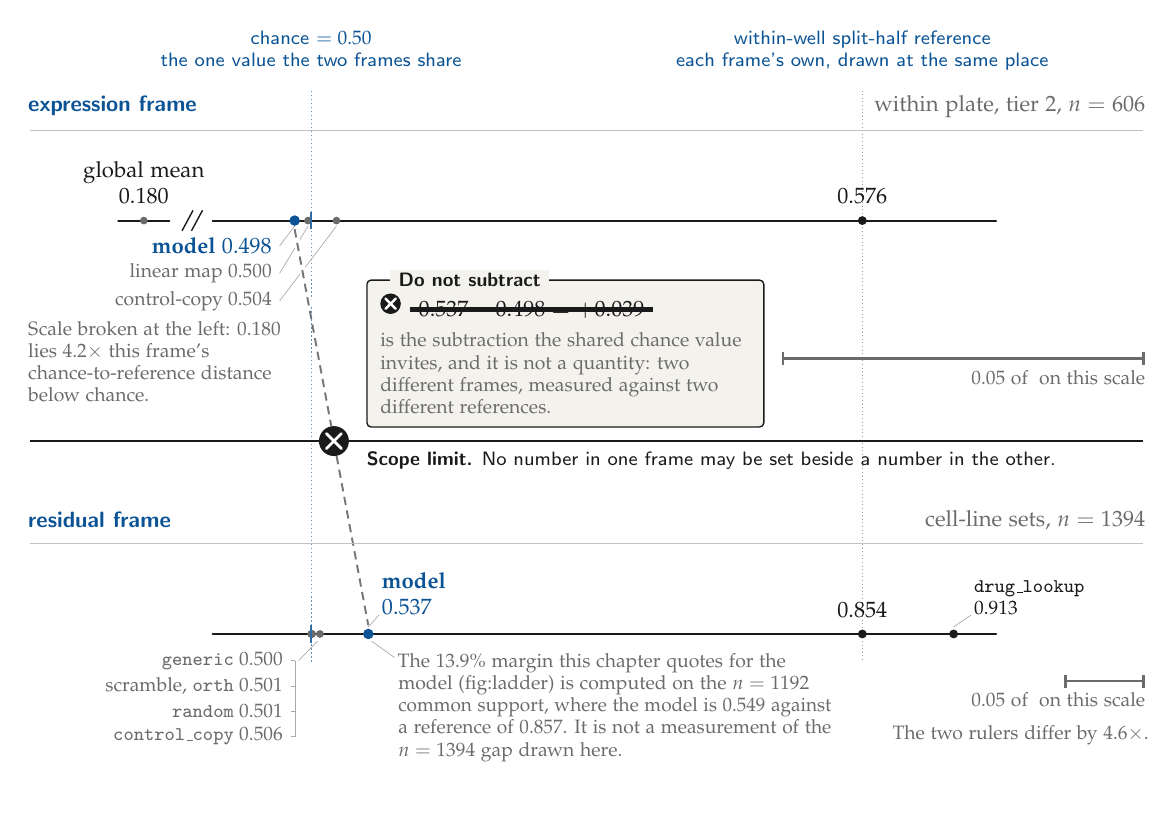
\begin{tikzpicture}[
  x=1cm, y=1cm,
  scaleline/.style={ink, line width=0.7pt, line cap=round},
  guide/.style={rulegrey, densely dotted, line width=0.3pt},
  chanceguide/.style={accent!65, densely dotted, line width=0.45pt},
  leader/.style={rulegrey!85, line width=0.25pt},
  headrule/.style={rulegrey!60, line width=0.3pt},
  hardrule/.style={ink, line width=1.0pt},
  connector/.style={ink!60, densely dashed, line width=0.7pt},
  calib/.style={quietink, line width=0.9pt, line cap=butt},
  fh/.style={font=\sffamily\footnotesize\bfseries, text=accent, inner sep=0pt},
  fhs/.style={font=\footnotesize, text=quietink, inner sep=0pt},
  gh/.style={anchor=north, font=\sffamily\scriptsize, text=accent,
             align=center, inner sep=1pt},
  val/.style={font=\footnotesize, text=ink, align=center, inner sep=1.5pt},
  arm/.style={font=\scriptsize, text=quietink, inner sep=1.5pt},
  armM/.style={font=\footnotesize\bfseries, text=accent, inner sep=1.5pt},
  note/.style={font=\scriptsize, text=quietink, align=flush left, inner sep=0pt},
  noteR/.style={font=\scriptsize, text=quietink, align=flush right, inner sep=0pt},
]

% ---- the bounding box IS the body block; nothing may stick out of it
\path (0.0000,1.60) rectangle (14.2000,11.3000);

% ================ the two alignment anchors
\node[gh] at (3.6000,11.3000) {chance $=0.50$\\ the one value the two frames share};
\node[gh] at (10.6000,11.3000) {within-well split-half reference\\ each frame's own, drawn at the same place};
\draw[chanceguide] (3.6000,10.5000) -- (3.6000,3.2500);
\draw[guide]       (10.6000,10.5000) -- (10.6000,3.2500);

% ================ UPPER SCALE -- expression frame
\node[fh,  anchor=west] at (0.0000,10.30) {expression frame};
\node[fhs, anchor=east] at (14.2000,10.30) {within plate, tier 2, $n=\num{606}$};
\draw[headrule] (0.0300,10.00) -- (14.1700,10.00);
\draw[scaleline] (2.35,8.8500) -- (12.30,8.8500);
\draw[scaleline] (1.15,8.8500) -- (1.80,8.8500);   % the broken stub
\draw[ink, line width=0.5pt] (1.96,8.7200) -- (2.10,8.9800);
\draw[ink, line width=0.5pt] (2.08,8.7200) -- (2.22,8.9800);
\fill[quietink] (1.4750,8.8500) circle (1.4pt);   % global mean, off scale
\fill[quietink] (3.5605,8.8500) circle (1.4pt);   % linear map
\fill[quietink] (3.9220,8.8500) circle (1.4pt);   % control-copy
\fill[ink]      (10.6000,8.8500) circle (1.6pt);   % within-well reference
\fill[accent]   (3.3904,8.8500) circle (1.9pt);   % model
\draw[accent!85, line width=0.5pt] (3.6000,8.7400) -- (3.6000,8.9600);
\node[val, anchor=south] at (1.4750,9.0000) {global mean\\ $0.180$};
\node[val, anchor=south] at (10.6000,9.0000) {$0.576$};
\draw[leader] (3.3904,8.7800) -- (3.20,8.5300);
\node[armM, anchor=east] at (3.16,8.5300) {model\;$0.498$};
\draw[leader] (3.5605,8.7800) -- (3.20,8.1800);
\node[arm, anchor=east] at (3.16,8.1800) {linear map\;$0.500$};
\draw[leader] (3.9220,8.7800) -- (3.20,7.8300);
\node[arm, anchor=east] at (3.16,7.8300) {control-copy\;$0.504$};
\node[note, anchor=north west, text width=3.30cm] at (0.00,7.58) {Scale broken at the left: $0.180$ lies $4.2\times$ this frame's chance-to-reference distance below chance.};
\draw[calib] (9.5900,7.10) -- (14.1700,7.10);
\draw[calib] (9.5900,7.02) -- (9.5900,7.18);
\draw[calib] (14.1700,7.02) -- (14.1700,7.18);
\node[noteR, anchor=north east] at (14.2000,6.96) {$0.05$ of $\NIR$ on this scale};

% ================ the subtraction the figure exists to forbid
\draw[white, line width=2.2pt] (3.3904,8.7400) -- (3.5864,7.7500);
\draw[connector] (3.3904,8.7400) -- (3.8555,6.2400);
\draw[connector] (3.9232,5.8600) -- (4.3259,3.7100);
\node[draw=ink, line width=0.5pt, rounded corners=1.5pt, fill=panelbg, inner sep=0.17cm, text width=4.70cm, anchor=south west, font=\scriptsize, text=quietink, align=flush left] (nosub) at (4.3000,6.2200) {\tikz[baseline=(eq.base)]{ \node[inner sep=0pt, font=\footnotesize, text=ink, anchor=west] (eq) at (0.50,0) {$0.537 - 0.498 = +0.039$}; \draw[ink, line width=1.6pt] ([xshift=-0.10cm]eq.west) -- ([xshift=0.10cm]eq.east); \fill[ink] (0.15,0.075) circle (0.130); \draw[white, line width=0.9pt, line cap=round] (0.085,0.010) -- (0.215,0.140); \draw[white, line width=0.9pt, line cap=round] (0.085,0.140) -- (0.215,0.010); }\\[3pt] is the subtraction the shared chance value invites, and it is not a quantity: two different frames, measured against two different references.};
\node[fill=panelbg, inner xsep=3pt, inner ysep=1pt, anchor=west, font=\sffamily\scriptsize\bfseries, text=ink] at ([xshift=0.30cm]nosub.north west) {Do not subtract};

% ================ the scope limit, drawn as a rule and not as a caption
\draw[hardrule] (0.0300,6.0500) -- (14.1700,6.0500);
\node[anchor=north west, font=\sffamily\scriptsize, text=ink, align=flush left, inner sep=0pt, text width=9.90cm] at (4.30,5.9200) {\textbf{Scope limit.} No number in one frame may be set beside a number in the other.};
% the connector is stopped at the rule, with the panel's own mark
\fill[ink] (3.8894,6.0500) circle (0.190);
\draw[white, line width=1.0pt, line cap=round] (3.7944,5.9550) -- (3.9844,6.1450);
\draw[white, line width=1.0pt, line cap=round] (3.7944,6.1450) -- (3.9844,5.9550);

% ================ LOWER SCALE -- residual frame
\node[fh,  anchor=west] at (0.0000,5.05) {residual frame};
\node[fhs, anchor=east] at (14.2000,5.05) {cell-line sets, $n=\num{1394}$};
\draw[headrule] (0.0300,4.75) -- (14.1700,4.75);
\draw[scaleline] (2.35,3.6000) -- (12.30,3.6000);
\fill[quietink] (3.6000,3.6000) circle (1.4pt);   % generic
\fill[quietink] (3.6113,3.6000) circle (1.4pt);   % scramble_orth
\fill[quietink] (3.6126,3.6000) circle (1.4pt);   % random
\fill[quietink] (3.7118,3.6000) circle (1.4pt);   % control_copy
\fill[ink]    (10.6000,3.6000) circle (1.6pt);   % within-well reference
\fill[ink]    (11.7597,3.6000) circle (1.6pt);   % drug_lookup
\fill[accent] (4.3259,3.6000) circle (1.9pt);   % model
\draw[accent!85, line width=0.5pt] (3.6000,3.4900) -- (3.6000,3.7100);
\draw[leader] (4.3259,3.6900) -- (4.46,3.8400);
\node[val, anchor=south west, align=left, text=accent, font=\footnotesize\bfseries] at (4.44,3.7800) {model\\ $0.537$};
\node[val, anchor=south] at (10.6000,3.7500) {$0.854$};
\draw[leader] (11.7597,3.6900) -- (11.98,3.8400);
\node[arm, anchor=south west, align=left, text=ink] at (11.96,3.7800) {\texttt{drug\_lookup}\\ $0.913$};
\draw[leader] (3.6818,3.5100) -- (3.44,3.26);
\draw[leader] (3.40,3.26) -- (3.40,2.29);
\draw[leader] (3.40,3.2600) -- (3.34,3.2600);
\node[arm, anchor=east] at (3.30,3.2600) {\texttt{generic}\;$0.500$};
\draw[leader] (3.40,2.9400) -- (3.34,2.9400);
\node[arm, anchor=east] at (3.30,2.9400) {scramble, \texttt{orth}\;$0.501$};
\draw[leader] (3.40,2.6200) -- (3.34,2.6200);
\node[arm, anchor=east] at (3.30,2.6200) {\texttt{random}\;$0.501$};
\draw[leader] (3.40,2.3000) -- (3.34,2.3000);
\node[arm, anchor=east] at (3.30,2.3000) {\texttt{control\_copy}\;$0.506$};
\draw[leader] (4.3659,3.5100) -- (4.66,3.30);
\node[note, anchor=north west, text width=5.50cm] at (4.70,3.36) {The $13.9\%$ margin this chapter quotes for the model (\cref{fig:ladder}) is computed on the $n=\num{1192}$ common support, where the model is $0.549$ against a reference of $0.857$. It is not a measurement of the $n=\num{1394}$ gap drawn here.};
\draw[calib] (13.1810,3.00) -- (14.1700,3.00);
\draw[calib] (13.1810,2.92) -- (13.1810,3.08);
\draw[calib] (14.1700,2.92) -- (14.1700,3.08);
\node[noteR, anchor=north east] at (14.2000,2.86) {$0.05$ of $\NIR$ on this scale};
\node[noteR, anchor=north east, text width=3.85cm] at (14.2000,2.44) {The two rulers differ by $4.6\times$.};
\end{tikzpicture}
%
% ---------------------------------------------------------------------------
% READY TO PASTE into Sections/04d-baselines.tex, at sec:res-summary, just after
% the paragraph "The same chance value, two different references".
%
% \begin{figure}[htbp]
% \centering
% \input{figs/two-scales}
% \caption[Two frames, one chance value]{\textbf{The two frames share a chance
% value and nothing else, and the shared value is exactly what makes the mistake
% easy.} Each scale is stretched so that chance falls at the same place in both
% and so that each frame's own within-well split-half precision reference falls
% at the same place as the other's. Nothing else is aligned, so the two frames
% carry different rulers --- the same $0.05$ of $\NIR$ is 4.6 times longer
% above than below --- and that differential stretch is the figure.
% \emph{Upper:} the expression frame, within plate, tier 2, $n = \num{606}$,
% where the model scores $0.498$ against a reference of $0.576$ and is matched by
% a drug-agnostic linear map ($0.500$) and a control-copy ($0.504$); the scale is
% broken at the left because the global mean, $0.180$, lies $4.2\times$ that
% frame's chance-to-reference distance below chance. \emph{Lower:} the residual
% frame, cell-line sets, $n = \num{1394}$, where the model scores $0.537$ against
% a reference of $0.854$, a training-only per-drug lookup reaches $0.913$ above
% that reference, and \texttt{generic}, \texttt{orth}, \texttt{random} and
% \texttt{control\_copy} all fall within $0.006$ of chance, one mark at this
% scale. Both references are within-well split-half precision figures --- two
% disjoint halves of one treated well --- and not biological replicates
% (\cref{sec:methods-data}). Chance is $0.50$ in both under the exchangeability
% condition audited in \cref{sec:res-metrics}, and because it is the one value
% the two frames share it is exactly what makes the struck-out subtraction in the
% middle of the figure easy to perform: $0.537$ and $0.498$ are not two attempts
% at one task, and the difference between them is neither an improvement nor a
% decline. Every value is a pooled mean drawn as a bare marker; no arm shown here
% is quoted with an interval at the pooled level, so none is drawn
% (\cref{tab:allarms}). The $13.9\%$ margin annotated below is computed on the
% $n = \num{1192}$ common support and is not a measurement of the
% $n = \num{1394}$ gap drawn here.}
% \label{fig:two-scales}
% \end{figure}
% ---------------------------------------------------------------------------

\caption[Two frames, one chance value]{\textbf{The two frames share a chance
value and nothing else, and the shared value is exactly what makes the mistake
easy.} Each scale is stretched so that chance falls at the same place in both and
so that each frame's own within-well split-half precision reference falls at the
same place as the other's; nothing else is aligned, so the two frames carry
different rulers --- the same $0.05$ of $\NIR$ is $4.6\times$ longer above than
below --- and that differential stretch is the figure. \emph{Upper:} the
expression frame, within plate, tier 2, $n = \num{606}$, where the model scores
$0.498$ against a reference of $0.576$ and is matched by a drug-agnostic linear
map ($0.500$) and a control-copy ($0.504$); the scale is broken at the left
because the global mean, $0.180$, lies $4.2\times$ that frame's
chance-to-reference distance below chance. \emph{Lower:} the residual frame,
cell-line sets, $n = \num{1394}$, where the model scores $0.537$ against a
reference of $0.854$, a training-only per-drug lookup reaches $0.913$ above that
reference, and \texttt{generic}, \texttt{orth}, \texttt{random} and
\texttt{control\_copy} all fall within $0.006$ of chance, one mark at this scale.
Both references are within-well split-half precision figures --- two disjoint
halves of one treated well --- and not biological replicates
(\cref{sec:methods-data}). Chance is $0.50$ in both under the exchangeability
condition audited in \cref{sec:res-metrics}, and because it is the one value the
two frames share it is exactly what makes the struck-out subtraction in the
middle of the figure easy to perform. Every value is a pooled mean drawn as a
bare marker; no arm shown here is quoted with an interval at the pooled level, so
none is drawn (\cref{tab:allarms}). The $13.9\%$ margin annotated below is
computed on the $n = \num{1192}$ common support and is not a measurement of the
$n = \num{1394}$ gap drawn here.}
\label{fig:two-scales}
\end{figure}

% PLACEMENT ONLY. The ledger was anchored two paragraphs and a scope-limit box
% lower down, past the point where a float 0.82 of the column high can still be
% taken: it was deferred, took a page to itself, and left the three lines that
% close the chapter alone on the page after it. Anchored here, at the sentence
% that announces it -- "What follows is a ledger of the principal comparison
% arms" -- it is offered a page earlier and heads a text page instead. Reading
% order is unchanged: the table still sets before the prose that reads it.
% Chapter 4 previously never \cref'd this table -- the nearest references were in
% ch.5 and the appendix, five and thirty-odd pages away. It is now \cref'd on
% both sides of the float, one page either side: in the frame-defining paragraph
% immediately above (the page before the table sets) and in "What the ledger
% deliberately leaves out" below. Verified page-neutral against a pristine build:
% same section page, same table page, same chapter-end page, same page count.
% ---------------------------------------------------------------------------
\begin{table}[htbp]
\begin{fullwidth}
\begin{threeparttable}
\caption{\textbf{The principal comparison arms on the calibrated metric, by
frame.} Chance is $0.50$ in both; reference rows are within-well split-half
precision figures, not biological replicates (\cref{sec:methods-data}). The final
expression rows show the $204$ conditions clearing the pre-set $0.80$
identifiability threshold, where a drug-agnostic control still matches the model.
Of the scramble strata, \texttt{near} ($0.550$) and \texttt{opposite} ($0.423$)
differ from chance in opposite directions while \texttt{orth} ($0.501$) is
empirically near chance here; because the strata are defined using true residual
geometry, \texttt{orth} is the least contaminated available comparator and not an
independently established null (\cref{sec:res-generalisation}).}
\label{tab:allarms}
\small
\begin{tabular}{llr>{\raggedright\arraybackslash}p{0.30\linewidth}}
\toprule
\thead{Frame} & \thead{Arm} & {\thead{$\NIR$}} & \thead{What it knows} \\
\midrule
\multirow{7}{*}{\shortstack[l]{expression\\(within plate,\\tier 2, $n=606$)}}
 & within-well reference & 0.576 & two disjoint halves of one treated well;
precision, not a replicate \\
 & control-copy & 0.504 & nothing; it reproduces the untreated cell \\
 & linear map & 0.500 & the control cell, no drug \\
 & \textbf{model} & \textbf{0.498} & control cell $+$ drug \\
 & global mean & 0.180 & nothing \\
 & \textbf{model}, identifiable stratum & \textbf{0.768} & the same model, on the
$204$ conditions whose own reference clears $0.80$ \\
 & control-copy, same stratum & 0.766 & nothing, and it matches the model
there \\
\midrule
\multirow{7}{*}{\shortstack[l]{residual\\(cell-line sets,\\$n=1394$)}}
 & within-well reference & 0.854 & two disjoint halves of one treated well; not a
replicate, and on the lookups' support, where it is $0.857$, the lookup exceeds
it \\
 & drug lookup (training-only) & 0.913 & this drug's residual from other cell
lines, on the $n = \num{1192}$ conditions admitting a lookup, where the model
scores $0.549$ \\
 & drug lookup, one line & 0.822 & the same, from one other cell line, same
support \\
 & \textbf{model} & \textbf{0.537} & control cell $+$ drug \\
 & scramble, \texttt{orth} partner & 0.501 & geometry-defined by residual cosine
to the target ($\cos \approx 0$); its own score is \emph{empirically} near chance
here \\
 & scramble, \texttt{opposite} partner & 0.423 & an active treatment, not a
null \\
 & generic response & 0.500 & nothing (the zero vector, by construction) \\
\bottomrule
\end{tabular}
\end{threeparttable}
\end{fullwidth}
\end{table}

\paragraph{The same chance value, two different references} Both use $0.50$ as
chance under the exchangeability condition audited in \cref{sec:res-metrics}.
\Cref{fig:two-scales} puts each frame on its own ruler, scaled so that chance and
that frame's own within-well precision reference fall at the same two places: the
$0.537$ in one frame and
the $0.498$ in the other are not two attempts at one task, and the difference
between them is neither an improvement nor a decline. Read each against its own
reference, the expression-frame model does not clear chance at all, and the
residual-frame model clears it on trained conditions only,
\ci{0.598}{0.549}{0.647} there against \ci{0.533}{0.492}{0.575} and
\ci{0.459}{0.404}{0.514} on the held-out splits, neither distinguishable from
$0.50$ (\cref{sec:res-generalisation}). The pooled $0.537$ is three-quarters
held-out condition, and no arm is quoted with an interval at the pooled level, so
it is quoted as a mean and not as a clearance.


\paragraph{And the margin between them has a support} What separates the frames
is a margin \cref{sec:res-lookup} sizes at $13.9\%$ of the distance from chance
to the reference, computed on the $n = \num{1192}$ common support where the model
scores $0.549$ against a reference of $0.857$, and not on the $n = \num{1394}$
whose $0.537$ and $0.854$ are quoted above.

\begin{scopelimit}[carried into \cref{sec:limitations}]
No number in one frame may be set beside a number in the other. Chance is $0.50$
in both, which is exactly what makes the mistake easy to make; the references
above chance are $0.854$ and $0.576$, and every distance quoted in this chapter is
a distance to its own frame's reference. Within the residual frame the same
applies to supports: $\num{1394}$, $\num{1192}$ and $\num{218}$ select conditions
by different rules, and rows on different supports are not comparable.
\end{scopelimit}

% ---------------------------------------------------------------------------
\paragraph{What the ledger deliberately leaves out} \cref{tab:allarms} omits the
\texttt{near} scramble, a deliberately weak test; \texttt{moa\_lookup}, whose
$n=218$ support is not comparable with the principal rows; the residual-frame
\texttt{control\_copy} and \texttt{random} negatives, which serve the calibration
diagnostic; and the field-attribution arms, whose non-neutral comparators leave
attribution unresolved. The expression-frame control-copy stays because it
carries the identifiable-stratum comparison, and \texttt{orth} and
\texttt{opposite} because their contrast exposes how comparator score depends on
partner geometry.

\paragraph{Five results are estimates, not predictor arms} They are stated
outside the ledger because nothing in it is their comparison set.

\begin{itemize}
\item \textbf{The metric audit.} Of the five metrics graded, $\NIR$ is the only
one whose $\DRF$ is positive, \ci{+0.635}{+0.604}{+0.663} across plates,
\ci{+0.545}{+0.516}{+0.569} within plate, \ci{+0.704}{+0.667}{+0.736} in the
residual frame; the other four are negative and exclude zero. Three,
$\paneltau$, \texttt{spearman\_expr} and $\DEdr$, are inverted rather than merely
uninformative, scoring an uninformative baseline above the positive control;
\texttt{weighted\_r2} sits closest to zero and its sign tracks cell count, so it
carries no directional claim (\cref{sec:res-metrics}).
\item \textbf{Representation and readout.} Drug identity is decodable from the
activations, and the generation readout consults it at one to two per cent of the
preference gap, a fifth or less of the pre-registered material margin, in one
training arm and at one rung of the displacement ladder; the chapter's weakest
load-bearing result (\cref{sec:res-mechanism}).
\item \textbf{Prompt sensitivity.} Re-encoding the target as the drug-specific
residual gives \ci{+0.0898}{+0.0291}{+0.1506} on trained conditions, clustered on
the drug. A budget-matched optimal-transport control clears zero too, at
\ci{+0.0292}{+0.0144}{+0.0441}, so the re-encoding is first in the sequence and
not uniquely responsible (\cref{sec:res-encoding}).
\item \textbf{Transfer.} \ci{\Tcoef = 0.553}{0.514}{0.593}, a cross-context
similarity coefficient and not a variance share (\cref{sec:res-transfer}).
\item \textbf{The channels.} Same-target retrieval is the strongest observed lead
on its restricted support; only that arm clears the relevance margin, on the
cell-line axis on all three constructions and not on the drug axis under either
estimand-correct null, on $18$ annotated drugs of which two are held out. The
arms differ in support, roster, partner count and annotation coverage, so this is
not an identified biological ranking (\cref{sec:res-scope}).
\end{itemize}

\noindent
The distance between the model and the least contaminated available scramble is
the prompt-sensitivity effect this work recovered; the distance between the model
and the lookup is what it did not.


% ===========================================================================
% 05-Limitations.tex. PRESENTATION ONLY. Every number, interval, hedge and
% conclusion is verbatim from v1. ONE \needsaudit, in "Cross-plate absolutes".
% ===========================================================================

\chapter{Limitations and future research directions}
\label{sec:limitations}
\framedecl{ER}

\begin{question}
Every measurement in this thesis was made on one atlas, one checkpoint and one
slice of both. Which of its conclusions are properties of the model, and which
are properties of that slice?
\end{question}

\noindent
A limitation is worth writing down when it changes what a number licenses.

% ===========================================================================
\section{Every result here is scoped, and the scopes differ}

\paragraph{Drug coverage} A study of $106$ drugs can establish that a model uses
the drug it is handed; it cannot describe how drugs in general behave. The
residual analysis uses $\num{620564}$ cells covering $106$ drugs across $50$
cell lines, roughly a tenth of the atlas's drug set, ample for testing
whether the model uses the drug and for measuring transfer but not a population
estimate. Claims about the \emph{distribution} of drug behaviours belong to the
broader characterisation, which used $\num{6628}$ conditions.

\paragraph{Only reproducible conditions} A residual that does not reproduce
between two halves of the same well is not a target anything could learn, so the
residual arm trains on the $50.5\%$ of conditions whose residual does reproduce,
$\num{2523}$ of $\num{4999}$ training conditions kept at $\cos > 0.109$, the
$95$th percentile of a null pairing half A of one condition with half B of
another.\gloss{reliability line}{The half-split cosine threshold above which a
condition's residual counts as reproducible.} The model was taught the
empirically reproducible fraction. Split-half retrieval establishes
discriminability of treated populations under this sampling design and cell
budget; it does not establish predictability from untreated input or
learnability.

A reliability filter might be expected to select \emph{toward}
context-in\-de\-pen\-dent conditions and bias the transfer coefficient upward.
It does the opposite. Unfiltered \ci{0.597}{0.563}{0.632}, filtered
\ci{0.553}{0.514}{0.593}; the filtered value is quoted, because disattenuation
is unstable at the very low reliabilities the filter removes.

That calculation's own filter is the inherited $\cos > 0.2$ line, where the
training set uses $0.109$, so the two estimates bracket the trained-on
population without reproducing it. The generation evaluation mismatches
differently again, applying $0.109$ to \texttt{train} and leaving the held-out
splits unfiltered. That one is load-bearing and is taken up below.

\paragraph{The intervals omit generation variance} The intervals here are
cluster-robust with each condition's score treated as fixed: two-way over
\emph{cell line} and \emph{treated well} on a $\min(G_{\textrm{line}},
G_{\textrm{well}}) - 1$ Student $t$ reference for the headline gaps, reported
again clustered on the \emph{drug}; multiway dyadic for the transfer
coefficient; a one-way clustered bootstrap, unit named, in a few tables.

They capture between-cluster variance and leave out the variance from sampling
the model's predictions. With four sampled generations per condition at temperature
$0.8$ in the residual-frame arms and eight in the expression-frame ones
(\cref{sec:methods-data}), that source is not negligible, and no across-seed
replication of the generation arms was run, deferred or planned. Every interval
quoted from a generation arm covers the sampling of conditions, cell lines and
wells, and stops there.

One measurement \emph{was} repeated across seeds, recorded so it is not mistaken
for the replication that was not run. The activation probe of
\cref{sec:res-mechanism} returned $+0.0197$, $+0.0118$ and $+0.0085$ on three
seeds, each excluding zero. Its spread does not transfer to $\NIR$ and does not
establish a scale for generation variance. Those runs share a checkpoint and
score teacher-forced log-probabilities, so their seed moves the prompts, the
partners and the bootstrap, and leaves both the weights and the sampled
prediction untouched. They are scored on $60$, $240$ and $240$ prompts in that order, so
the largest of the three effects is also the smallest-$n$ one.

\paragraph{No training run was repeated} The seeds above move prompts,
partners and resampling. None of them moves the weights. Every arm here was
trained once, from one base checkpoint under identical hyperparameters
(\cref{tab:trainconfig}), so each dissociation this thesis rests on --- the
residual re-encoding against the standard target, and the optimal-transport
target against both --- compares one training run with one training run. A
second run of the same arm under a different data order would land on a
different checkpoint and score differently, and the size of that difference was
never measured here. It is therefore not covered by any interval in this
document: the intervals quantify sampling over conditions, cell lines and wells,
and a between-arm gap of the size reported would survive or fail a training
replication that nobody has run. The ten-epoch diagnostic varies the horizon and
not the seed, so it bounds undertraining and not run-to-run spread. What this
costs is specific rather than general: the \emph{direction} of the re-encoding
effect is corroborated by the token-divergence measurement, which needs no
model at all, but the \emph{magnitude} of every arm-to-arm difference is an
n-of-one comparison.

\paragraph{A swing that looked like generation variance and was not} Unseeded
generation is the kind of defect that surfaces as an unstable number, and once
it seemed to.

\begin{withdrawn}{seed instability in the held-out-drug control}
Two superseded evaluations of the held-out-drug control returned values of
$\gap$ far enough apart to be recorded as evidence of seed instability. Only one
of the pair survives in the results archive, so the size of the swing is no
longer quotable. The diagnosis was wrong. It named the trigger and missed the
cause.
\end{withdrawn}

Both of the superseded figures are gaps against the \texttt{opposite} swap, which
\cref{sec:res-generalisation} shows is not a null; it carries a term for how far
the \emph{partner} drug was pushed the wrong way, which changes with the
draw.\seealso{\cref{sec:res-generalisation}, where a neutral stratum replaces
\texttt{opposite} as the comparator} On the canonical evaluation the same
control reads $+0.0379$ against \texttt{opposite} and
\ci{-0.0315}{-0.0836}{+0.0206} against the neutral stratum, clustered two-way on
cell line and well.

Two mechanisms were at work, and both are now addressed. \texttt{do\_sample}
advanced from global torch state, so the two arms of a contrast were drawn from
different points of one
stream; each call now seeds its own generator from (condition, arm, batch), and
the comparator has been corrected. The general caution stands regardless; this
swing is no longer evidence for it.

\paragraph{Pseudobulk resolution} Residuals are condition-level pseudobulks over
$\geq 40$ treated cells, so single-cell heterogeneity of the response is not
modelled in this frame. Earlier project results show why: at single-cell
resolution the drug moves a cell less than noise does (SNR $\approx 0.75$,
median $0$ differentially expressed genes at FDR $q<0.05$).

\paragraph{Cross-plate absolutes} Residual-space scores use comparison sets
grouped by cell line, not by plate. The \emph{difference} $\gap$ is leak-immune,
since both arms share the same control cell. The absolute $\NIR$ values are a
different matter.

\cref{sec:methods-residual} argues the grouping is admissible because the
plate-scoped generic has already subtracted each plate's mean response from
truths and predictions alike. But it removes plate structure in expectation
only, and the generic is estimated from a small plate group, so some may survive
in an individual residual. The rescore that would size what survives, regrouping
the generation-free arms within plate, needs no GPU time and was not run.

What exists instead is one-sided. \cref{tab:plateleak} bounds it from
above.\framecue{\Eframe}{the plate-leak audit} In the expression frame with no
generic subtracted, holding the plate constant moves a drug-agnostic
\needsaudit[same construction as the DRF negative control]{mean baseline} from
$0.399$ to $0.161$ and the precision reference from $0.625$ to $0.575$ --- the
yardstick falls with the baseline (\cref{fig:plateleak}), so the leak is not an
offset one side of a comparison could be corrected by.
Residual-frame absolutes should be read within their own frame and never set
beside a within-plate number.

\begin{table}[htbp]
\centering
\begin{threeparttable}
\caption{\textbf{Expression-frame $\NIR$, the leak audit.} A drug-agnostic mean
baseline more than doubles its score when the plate is free to vary. The
precision reference falls once the plate is held constant, because batch
structure was inflating it too.}
\label{tab:plateleak}
\footnotesize
\setlength{\tabcolsep}{6pt}
\begin{tabular}{@{}lrr@{}}
\toprule
\thead{Predictor (drug-agnostic)} & \thead{cross-plate}
  & \thead{within plate} \\
\midrule
mean baseline & 0.399 & \textbf{0.161} \\
control-copy & 0.551 & 0.510 \\
\midrule
precision reference (within-well split-half) & 0.625 & 0.575 \\
fraction of drugs at chance & 43\% & 49\% \\
\bottomrule
\end{tabular}
\begin{tablenotes}[flushleft]\footnotesize
\item A wider diagnostic run than the $n = 606$ tier-2 benchmark the blindness
verdict is stated on, at $n = \num{1163}$ cross-plate and $n = 998$ within
plate. Holding the plate constant costs every condition with no same-plate
comparison set, so the within-plate column is a subset of the cross-plate one
rather than the same conditions rescored.
\item Its within-plate figures therefore sit slightly off \cref{tab:allarms},
control-copy $0.510$ against $0.504$, mean baseline $0.161$ against $0.180$,
precision reference $0.575$ against $0.576$.
\end{tablenotes}
\end{threeparttable}
\end{table}

\begin{figure}[htbp]
\centering
% drawn at 142mm by thesis_v2/figs/plateleak.py, the width of the measure; no
% width= key, so it is placed at scale 1.0 and its type prints at the point
% sizes it was set in. Values in figs/fig-plateleak.json, read from
% RESULTS_cluster/leak_crossplate.json and RESULTS_cluster/leak_sameplate.json,
% tiers.tier2_unseen_drugs.agg, the *_nir_expr entries only.
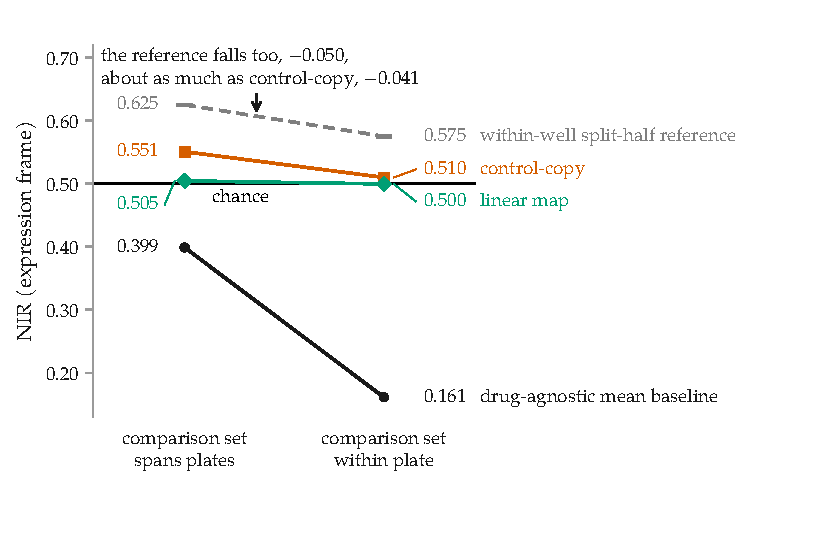
\includegraphics{fig-plateleak}
\caption[Holding the plate constant lowers the reference too]{\textbf{The batch
shortcut inflates the precision reference as well as the baseline, so it is not
an offset that could be subtracted from one side of a comparison.}
Expression-frame $\NIR$, tier 2 unseen drugs, drug-agnostic arms only: the same
audit as \cref{tab:plateleak}, with the linear map read from the same block of
the same two records. Forcing the comparison set within plate collapses a mean
baseline that carries no drug information whatsoever, $0.399$ to $0.161$, and
leaves control-copy close to where it was, $0.551$ to $0.510$ --- but it also
lowers the within-well split-half precision reference, $0.625$ to $0.575$, by
about as much as it lowers control-copy. That reference is the yardstick these
expression-frame numbers are read against, so the leak has no one side to be
corrected on. The two columns are not the same conditions: holding the plate
constant costs every condition with no same-plate comparison set, so the
within-plate column is a \emph{subset} --- $n = 998$ conditions, $46$ drugs,
$41$ cell lines --- of the cross-plate column's $n = \num{1163}$, $50$ drugs and
$43$ cell lines, and each segment joins two scorings of overlapping but unequal
populations rather than one set of conditions rescored. The marks are bare
because neither record carries an interval for these quantities, each entry
being a value and its $n$, and this document draws only $95\%$ bootstrap
intervals clustered over cell lines. The rank-frame variants stored beside these
values are a different frame and are not drawn, and none of the values here may
be set beside a residual-frame number.}
\label{fig:plateleak}
\end{figure}

\paragraph{Frame coverage} The drug-specific residual is
$\lVert\resid\rVert/\lVert\shift\rVert = 0.786$ of the shift against $0.620$
for the generic programme and batch, and the two are essentially orthogonal, the
shift's energy decomposing into residual $0.621$, generic $0.390$ and a cross
term of $-0.011$, summing to $1.000$. The frame covers $62.1\%$ of the shift's
\emph{energy}, a real but not total share, and every result here should be read
within that bound. The generic $39.0\%$ is drug-agnostic and trivially matched,
part of what a drug-agnostic predictor supplies on absolute-accuracy metrics,
though the generic programme is not what saturates $\DEdr$; reversion toward a
central point is (\cref{sec:res-metrics}).

\paragraph{The splits are scored on different populations} The within-well
split-half precision reference differs sharply across the three splits as
scored, $0.956$ on \texttt{train}, $0.824$ on \texttt{unseen\_combo} and $0.836$
on \texttt{unseen\_drug}. The obvious reading is that held-out conditions carry
less recoverable signal. That reading is wrong.

It is the selection asymmetry noted above. \texttt{train} is drawn from a pool
already filtered at the $0.109$ line, and none of its $300$ scored conditions
falls at or below it, while the held-out splits are unfiltered and still contain
conditions whose two halves disagree outright. Impose the training line on all
three and the references agree at $0.955$, $0.961$ and $0.960$, a spread of
$0.006$ where there had been $0.132$ (\cref{fig:splitref}). Matched on
reproducibility, a held-out condition is as recoverable as a trained one.

% The float that stood here (193-249 of the previous revision) is now
% figs/splitref.tex. It moved out of the section for the same reason the
% other reworked figures did -- the drawing carries 70 lines of its own
% rationale, which does not belong in the prose -- and it lost its
% \begin{fullwidth} on the way: it reserved 174mm, drew 150.2mm, and cost
% this page its margin column to show six numbers the caption already states.
% It now draws 132.9mm inside the 142mm measure.
% ===========================================================================
% splitref.tex -- the within-well split-half reference, as the three splits are
% actually scored and with the resolved +0.1086 reliability line imposed on all
% three.
% \input by Sections/05-Limitations.tex. Compiles against thesis_v2/preamble.tex
% and nothing else. Every number in the drawing is written by
% figs/splitref_numbers.py into figs/fig-splitref.json; run that script if the
% source records ever change, and paste its "TikZ dot values" block below.
%
% STALE GENERATOR -- READ BEFORE RE-RUNNING. splitref_numbers.py:57 hardcodes
% REPRO_LINE = 0.109 and its own comment (:54-56) says 0.109 was chosen because
% it "reproduces all three printed values". That is backwards: the line was
% fitted to the prose rather than taken from the definition, and the prose value
% it was fitted to is the one that is wrong. Panel B below is now drawn at the
% resolved +0.1086 line the document actually defines (see THE LINE). Re-running
% the script as it stands will silently revert this file. Set REPRO_LINE
% = 0.1086 there first, and regenerate figs/fig-splitref.json, which still
% records the superseded 0.109 reconstruction.
%
% v1's version sat inline in Sections/05-Limitations.tex at lines 193-249.
% Four things were wrong with it and are fixed here.
%
%   1. IT PAID FOR FULLWIDTH AND DID NOT USE IT. The old float opened
%      \begin{fullwidth} -- 174mm, and by the preamble's own rule the page
%      carrying one may then carry no margin note -- and drew 150.2mm. It shows
%      six numbers, all six of which its own caption already states, so it was
%      buying 32mm of extra measure to repeat the caption. This draws inside the
%      142mm body measure (see MEASURED below) and that page keeps its margin
%      column.
%
%   2. THE RIGHT-HAND BRACE WAS A DEGENERATE GLYPH. Three values spanning
%      0.956-0.961 on an axis running 0.82-0.98 collapse a
%      decorations.pathreplacing brace to about 1.5pt of path, shorter than its
%      own 3.5pt amplitude, and pgf draws the two halves overlapping: it printed
%      as a stray chevron beside "0.006". A brace that renders as a chevron is
%      worse than no brace. Both spans are now square brackets -- a form that
%      degrades gracefully, so the SAME mark is used in both panels and the
%      reader compares 47.8mm of bracket against 1.8mm of bracket directly.
%      Correspondingly the three converging leaders on the right panel's three
%      near-coincident dots are gone: a single block set hard against the
%      cluster lists all three values in the dots' own top-to-bottom order, so
%      it reads as the cluster magnified rather than as a legend.
%
%   3. NEITHER PANEL SAID WHAT WAS ON THE VERTICAL AXIS. The caption called it
%      "the reference" and the drawing named nothing. There is now a rotated
%      axis title naming the estimator and its frame.
%
%   4. THE TRUNCATION WAS SILENT. The axis runs 0.82-0.98 -- 16 points of a
%      100-point scale -- and that truncation is most of why the 0.132 spread
%      looks dramatic. Both panels share the scale, so the before/after
%      comparison is honest, but the reader has to be told. The axis is drawn
%      BROKEN, with 0.50 (chance, the bottom of the NIR scale's meaningful
%      range) marked below the break, and the caption states the range in words.
%
% GEOMETRY. x and y are both 1mm, so every coordinate below is a millimetre and
% the numbers can be checked against the MEASURED reading. \yv maps a reference
% value onto the axis: \lo..\hi spans \H mm.
%
%   spine            x = 7.5, y = 0 (0.82) .. 58 (0.98)
%   break            gap y = -4 .. 0, two slashes across it, stub -8 .. -4
%   panel A          bracket x = 13, dots x = 36, names from 38.5, values to 66
%   divider          x = 68.5
%   panel B          bracket x = 88, dots x = 91.5, value block from x = 94.5
%   gridlines        stop at x = 94, clear of the value block, uniform length
%
% The two brackets sit on OPPOSITE sides of their dot columns and that is
% deliberate. Panel A's is 47.8mm tall and reads as a measure from anywhere;
% panel B's is 1.8mm and would read as a stray mark if it were the 23mm from
% its dots that panel A's is, so it is set hard against them and its label is
% thrown outward instead. Same mark, same weight, same colour; only the side
% differs, and the two lengths stay directly comparable across the divider.
%
% The two lower dots of panel A sit 0.0127 apart, which is 4.62mm here, against
% a \scriptsize line box of 3.35mm -- so both labels sit at their own dot's
% height and NO leader is needed on the left panel either. That clearance is
% why \H is 58 and not the 52 the old version used.
%
% MEASURED, not estimated. figs/_harness_splitref.tex \input s this file against
% the real preamble, captures the float into a box with \caption and \label
% gobbled, and \typeout s \wd. Reading:
%   tikzpicture  377.33pt = 132.90mm wide, 220.73pt = 77.74mm tall
%   \textwidth   404.03pt = 142.00mm
%   fills 93.4% of the measure, 26.70pt = 9.39mm of slack.
% The build's overfull-hbox gate is 0; this figure contributes none. The
% fullwidth version it replaces drew 150.2mm against a 174mm allowance.
%
% NUMBERS. Panel A is read straight from CANONICAL_NUMBERS.json -> ceilings{}.
% Panel B is reconstructed from re_v3.json -> records[] at repro_cos > 0.1086;
% no file in RESULTS_cluster holds those three values. figs/fig-splitref.json
% carries the full provenance, and is STALE: it still describes the superseded
% 0.109 reconstruction (299 / 394 / 111 kept, train 0.955).
%
% THE LINE. 04c-reencoding.tex:212-213 defines it as the measured null's 95th
% percentile, "+0.109, resolving to +0.1086", and the document is consistent at
% 0.1086, not at 0.109:
%   - 04c:220-221  "Of the 300 scored training conditions ... none falls at or
%                  below the resolved +0.1086." The train minimum repro_cos in
%                  re_v3.json is 0.10892294 -- above 0.1086, BELOW 0.109. At
%                  > 0.109 the figure dropped exactly the condition the text
%                  says is not dropped.
%   - 04c:959      "499 conditions sit below the +0.1086 line" on unseen_combo,
%                  i.e. 396 of 895 kept. The source count of records under
%                  0.1086 is exactly 499; under 0.109 it is 501, giving 394.
%   - 04c:957-958  "train is by construction the reliability-surviving
%                  population", so imposing the line on train must not move
%                  train. At 0.1086 it does not: panel B's train is the same
%                  0.9555006 as panel A's, to the last digit. At 0.109 it moved.
% Recomputed from re_v3.json at repro_cos > 0.1086: kept 300 / 396 / 111, means
% 0.9555006 (train), 0.9605642 (unseen_combo), 0.9597734 (unseen_drug).
%
% TWO NUMBERS THIS FIGURE PRINTS THAT THE PROSE CONTRADICTS. Neither is
% arbitrated here; both are reported upward. The figure does not invent a third
% reading of either.
%   (a) train, panel B. Drawn and printed 0.956, the value the resolved line
%       gives. The prose still prints 0.955 at 04c-reencoding.tex:883 and
%       05-Limitations.tex:224, both inherited from the 0.109 reconstruction.
%       Those two sites need the same correction; they are outside this file.
%   (b) the right-hand spread, printed 0.006. Under the old 0.109 line that was
%       max(rounded) - min(rounded) = 0.961 - 0.955, the raw spread being
%       0.00517. Under the resolved line BOTH conventions give 0.005: the raw
%       spread is 0.0050636, and max(rounded) - min(rounded) = 0.961 - 0.956.
%       So 0.006 is no longer derivable at the line the document defines. It is
%       nevertheless what the prose prints in three places
%       (04c-reencoding.tex:884, 05-Limitations.tex:225 and 03-Apparatus.tex:378,
%       the last a table note in the apparatus chapter), so it is left standing
%       here rather than silently changed to 0.005 -- changing it would put the
%       figure at odds with the prose in three places, and the spread is a
%       claim. FLAGGED, NOT FIXED.
% The left-hand 0.132 is the raw spread rounded and is unaffected.
% ===========================================================================
\begin{figure}[htbp]
\centering
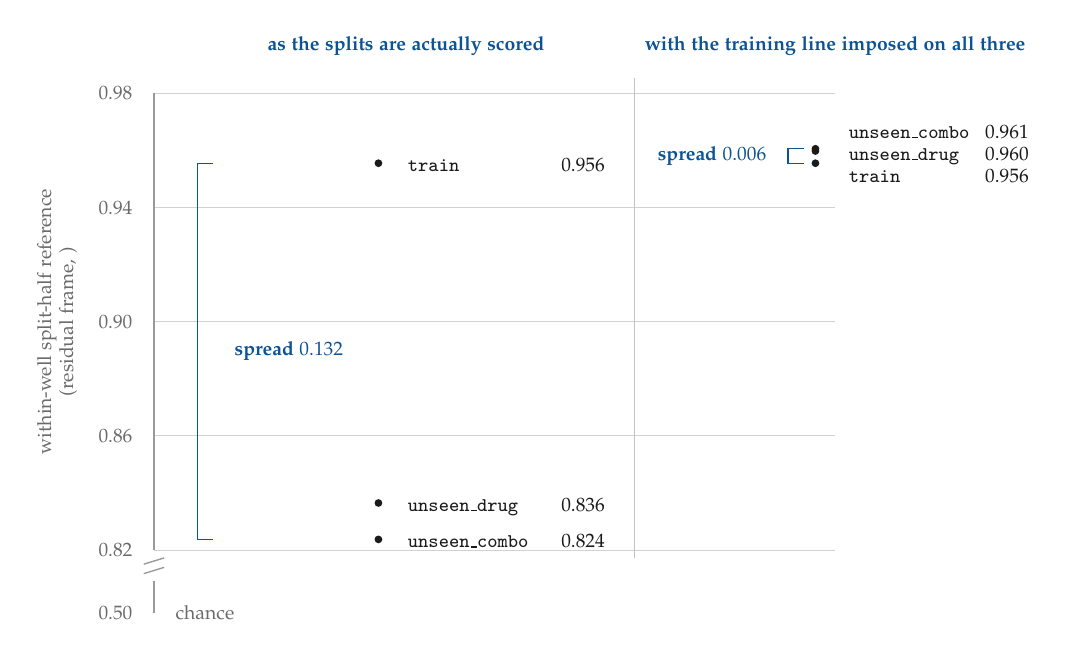
\begin{tikzpicture}[x=1mm, y=1mm, font=\small]
  % --- the constants every coordinate is derived from ----------------------
  \def\lo{0.82}\def\hi{0.98}\def\H{58}
  \newcommand{\yv}[1]{{(#1-\lo)/(\hi-\lo)*\H}}
  \def\ax{7.5}          % spine
  \def\bra{13}\def\dota{36}\def\laba{38.5}\def\vala{66}
  \def\divx{68.5}
  \def\brb{88}\def\dotb{91.5}\def\blk{94.5}
  \def\srf{2}           % bracket serif length, both panels

  \tikzset{
    grid/.style   ={draw=rulegrey!45, line width=0.3pt},
    spine/.style  ={draw=rulegrey, line width=0.5pt},
    tick/.style   ={font=\scriptsize, text=quietink},
    dot/.style    ={fill=ink},
    % text height/depth normalised so a \texttt name and a maths value set at
    % the same y sit on the same baseline; without it Inconsolata's box and the
    % maths box differ by 0.7pt and the three rows print visibly askew.
    lbl/.style    ={font=\scriptsize, text=ink,
                    text height=1.55ex, text depth=0.30ex},
    blk/.style    ={font=\scriptsize, text=ink},
    span/.style   ={draw=accent, line width=0.5pt},
    strong/.style ={font=\scriptsize\bfseries, text=accent}}

  % ---- 1. the shared scale ------------------------------------------------
  % One axis serves both panels; that is the argument, so it is drawn once.
  \foreach \v in {0.82,0.86,0.90,0.94,0.98}{
    \draw[grid] (\ax,\yv{\v}) -- (94,\yv{\v});
    \node[tick, anchor=east] at (\ax-1.5,\yv{\v}) {$\v$};}

  \draw[spine] (\ax,0) -- (\ax,\H);
  % the break, and chance below it. 0.50 is the foot of the NIR scale's
  % meaningful range and it is 32 points below anything drawn, so it is marked
  % past a break rather than pretended onto the plotted span.
  \draw[spine] (\ax,-8) -- (\ax,-4);
  \draw[spine] (\ax-1.3,-3.0) -- (\ax+1.3,-2.2);
  \draw[spine] (\ax-1.3,-1.8) -- (\ax+1.3,-1.0);
  \node[tick, anchor=east] at (\ax-1.5,-8) {$0.50$};
  \node[tick, anchor=west] at (\ax+1.5,-8) {chance};

  \node[rotate=90, anchor=south, font=\scriptsize, text=quietink, align=center]
    at (-1,29) {within-well split-half reference\\(residual frame, $\NIR$)};

  \draw[draw=rulegrey!60, line width=0.4pt] (\divx,-1) -- (\divx,60);

  \node[strong, anchor=south] at (39.5,61.5) {as the splits are actually scored};
  \node[strong, anchor=south] at (94,61.5)
    {with the training line imposed on all three};

  % ---- 2. panel A: the reference as each split is actually scored ---------
  % values: CANONICAL_NUMBERS.json -> ceilings{}
  % Name anchored west at \laba, value anchored EAST at \vala, so the three
  % values line up in a column despite the three split names differing by six
  % characters. Left-setting the whole label leaves them ragged.
  \fill[dot] (\dota,\yv{0.955501}) circle (1.4pt);
  \fill[dot] (\dota,\yv{0.836477}) circle (1.4pt);
  \fill[dot] (\dota,\yv{0.823720}) circle (1.4pt);
  \node[lbl, anchor=west] at (\laba,\yv{0.955501}) {\texttt{train}};
  \node[lbl, anchor=west] at (\laba,\yv{0.836477}) {\texttt{unseen\_drug}};
  \node[lbl, anchor=west] at (\laba,\yv{0.823720}) {\texttt{unseen\_combo}};
  \node[lbl, anchor=east] at (\vala,\yv{0.955501}) {$0.956$};
  \node[lbl, anchor=east] at (\vala,\yv{0.836477}) {$0.836$};
  \node[lbl, anchor=east] at (\vala,\yv{0.823720}) {$0.824$};

  \draw[span] (\bra+\srf,\yv{0.955501}) -- (\bra,\yv{0.955501})
           -- (\bra,\yv{0.823720}) -- (\bra+\srf,\yv{0.823720});
  % 0.889610 and 0.958032 below are the MIDPOINTS of the two spans, used to
  % place each label at the middle of its own bracket. They are geometry, not
  % data, and appear nowhere in fig-splitref.json.
  \node[strong, anchor=west] at (\bra+\srf+1.5,\yv{0.889610}) {spread $0.132$};

  % ---- 3. panel B: the same reference, training line imposed on all three --
  % values: reconstructed from re_v3.json -> records[] at repro_cos > 0.1086,
  % the resolved line of 04c-reencoding.tex:212-213. Kept 300 / 396 / 111.
  % train is 0.955501 -- byte-identical to panel A's train above, because all
  % 300 train conditions clear the line. That identity is the point: the line
  % selects train, so imposing it on train cannot move train.
  \fill[dot] (\dotb,\yv{0.960564}) circle (1.4pt);
  \fill[dot] (\dotb,\yv{0.959773}) circle (1.4pt);
  \fill[dot] (\dotb,\yv{0.955501}) circle (1.4pt);

  % Bracket hard against the dots, opening toward them; label thrown left.
  \draw[span] (\brb+\srf,\yv{0.960564}) -- (\brb,\yv{0.960564})
           -- (\brb,\yv{0.955501}) -- (\brb+\srf,\yv{0.955501});
  % 0.006 is the prose's number, not this panel's: see (b) in the header. The
  % bracket it labels spans 0.0050636, i.e. 0.005.
  \node[strong, anchor=east] at (\brb-1.5,\yv{0.958032}) {spread $0.006$};

  % Three dots 1.8mm apart cannot carry three leaders, and a leader short enough
  % to reach a block set beside them is indistinguishable from a hyphen. So: no
  % leader. One block, hard against the cluster with nothing else within 25mm of
  % it, listing all three in the dots' own top-to-bottom order, so it reads as
  % the cluster magnified rather than as a legend.
  \node[blk, anchor=west] at (\blk,\yv{0.958032})
    {\begin{tabular}{@{}l@{\hspace{2mm}}l@{}}
       \texttt{unseen\_combo} & $0.961$\\
       \texttt{unseen\_drug}  & $0.960$\\
       \texttt{train}         & $0.956$
     \end{tabular}};
\end{tikzpicture}
\caption[The split references, before and after matching]{\textbf{The three
splits do not differ in recoverable signal; they differ in which conditions were
allowed into them.} The vertical axis is the within-well split-half precision
reference --- one half of a condition's cells scored against the other half's
truth, in the residual frame, on the $\NIR$ scale --- and it is
\emph{truncated} to $0.82$--$0.98$, a sixth of the scale; chance is $0.50$,
marked below the axis break and far under everything drawn. Both panels share
that truncated scale, so the two spans may be read against each other. Left,
the reference as each split is actually scored, $0.956$ on \texttt{train}
against $0.824$ and $0.836$ on the held-out splits, a spread of $0.132$. Right,
the same reference with the resolved $+0.1086$ reliability line imposed on all
three, $0.956$, $0.961$ and $0.960$, a spread of $0.006$; at this scale the
three sit inside a bracket two millimetres tall, so they are listed beside the
cluster in
their own order rather than labelled in place. The left-hand spread is a
selection artefact. The markers are bare: no interval is carried for this
reference in the source record, and none is drawn rather than invented.}
\label{fig:splitref}
\end{figure}


\emph{Those conditions carry less signal} is therefore not a reason to discount
a held-out shortfall, and this thesis nowhere uses it as one. What survives is
narrower and binding. The matched-population rescore covered the precision
reference only. The model's own arms were never rescored, so what the held-out
shortfall becomes once the populations agree is not reported here, and the
training-exposure contrast of \cref{sec:res-generalisation} inherits the
mismatch.

% PLACEMENT ONLY. Eight lines and a framed header, and it was splitting five and
% three across the page turn, so the header sat with half its own text and the
% rest arrived under the running head as an unlabelled fragment. 11 lines is the
% box entire.
\needspace{11\baselineskip}%
\begin{scopelimit}[discharges the limit carried from \cref{sec:res-lookup}]
Three selection rules are in force at once, and no result computed under one of
them may be set beside a result computed under another. A raw score read across
the three splits is not answering the same question on each, because the splits
were filtered by different rules. An absolute $\NIR$ computed with the
comparison set grouped by cell line is not comparable with one computed within
plate. And a per-drug lookup is the bar for a drug that was \emph{seen} in
training and is being asked about a new context: no lookup exists for a drug
that never appeared in training, so that regime keeps its own bar, set in
\cref{sec:res-scope}.
\end{scopelimit}

% ===========================================================================
\section{What the unseen-drug arm licenses}

Two defects in the unseen-drug arm must be stated. A third, the comparator, was
found and corrected, and \cref{sec:res-generalisation} reports the arm against
the neutral stratum throughout.

\paragraph{The design leaks the drug's class} Holding out a drug does not
remove everything the model knows about it. The prompt contains
\texttt{Mechanism: \{moa\}}, so a held-out drug still arrives with its class
label. The correct design is leave-one-\emph{mechanism}-out.

The leak is measured, and the measurement is not clean. Scrambling the
\texttt{Mechanism} field alone moves the model's $\NIR$ by
\ci{+0.0303}{-0.0078}{+0.0685} ($n = \num{738}$, clustered on drug and well), an
interval containing zero. That understates the channel; it does not bound it,
because this row's swap partner scores $0.520$, above chance, and a comparator
above chance suppresses the gap (\cref{tab:fieldattribution}, Panel~B). A
mechanism-only lookup is the same measurement from the other side and equally
inconclusive. Pooled over the $n = \num{218}$ conditions on which both are
scored, model $-$ \texttt{moa\_lookup} $=$ \ci{+0.044}{-0.048}{+0.135},
clustered two-way on cell line and well, spans zero, so the comparison settles
nothing in either direction.

On \texttt{unseen\_drug}, the split where it would matter, the mechanism lookup
is ahead of the model by $0.099$ on $44$ conditions; in the contrast's reported
direction, model minus lookup is \ci{-0.099}{-0.222}{+0.008}, clustered on cell
line, spanning zero and far too wide to settle anything. That measurement has no
power at exactly the point where the design defect bites. It is not evidence
that the leak is doing work. The design is wrong, the arm cannot say what the
wrongness cost, and its proper use is as an instrument control.

\paragraph{It is underpowered by construction} The half-width on the
\texttt{unseen\_drug} gap is $\pm 0.052$ clustered two-way on cell line and
well, and $\pm 0.073$ clustered on the drug; the smallest effect detectable at
$80\%$ power is $\approx 0.079$. The largest effect the mechanism channel could
deliver is the distance from chance to \texttt{moa\_lookup}, which scores
$0.552$ pooled across splits against a chance value of $0.500$, so $\approx
0.052$. The arm \emph{cannot} detect the largest effect it could plausibly be
measuring (\cref{fig:power}).

% ===========================================================================
% power.tex -- the unseen-drug arm's detection floor against the largest
% effect the mechanism channel could plausibly deliver.
% \input by Sections/05-Limitations.tex, in "It is underpowered by
% construction". Compiles against thesis_v2/preamble.tex and nothing else;
% no \includegraphics, no external file read at build time.
%
% WHY THIS FIGURE EXISTS. The passage it sits in makes its argument out of
% four numbers delivered in four separate sentences (0.052, 0.073, 0.079,
% 0.052-as-largest-effect). The conclusion -- the arm cannot detect the
% largest effect it could plausibly be measuring -- only follows once all
% four are on one scale. On one scale it is a picture: the bar ends before
% the threshold begins.
%
% ---------------------------------------------------------------------------
% EVERY NUMBER DRAWN, ITS SOURCE, AND THE THESIS SENTENCE IT MUST MATCH.
% Sibling power.json records the same list machine-readably.
%
%  threshold (dashed accent rule)      0.07897560995161473
%      RESULTS_cluster/CANONICAL_NUMBERS.json
%          .detection_limit.detectable_at_80pc_power
%      (same object carries .split = "unseen_drug", .n = 199,
%       .observed = 0.45889838436740604, .half_width = 0.05528292696613031;
%       the observed NIR and that half_width are NOT drawn -- this is a
%       difference axis and 0.4589 is an absolute NIR.)
%      Sections/05-Limitations.tex:310-311 "the smallest effect detectable
%      at $80\%$ power is $\approx 0.079$".                        MATCHES.
%
%  bar length                          0.05201514916327314
%      = 0.5520151491632731 - 0.500
%        RESULTS_cluster/CANONICAL_NUMBERS.json .means_all.moa_lookup
%        = RESULTS_cluster/re_v3.json .means.moa_lookup   (identical to 16 sf)
%        chance 0.500 is a definition: both frames are two-alternative
%        retrievals (preamble/frames.tex, Sections/03-Apparatus.tex).
%      Sections/05-Limitations.tex:311-314 "The largest effect the mechanism
%      channel could deliver is the distance from chance to
%      \texttt{moa\_lookup}, which scores $0.552$ pooled across splits
%      against a chance value of $0.500$, so $\approx 0.052$."      MATCHES.
%      0.552 and 0.500 are absolute NIR values and are therefore stated in
%      the caption only; the drawing carries the difference and nothing else.
%
%  point estimate (filled marker)     -0.03148175705606285
%      CANONICAL_NUMBERS.json .splits.unseen_drug.gap
%      = re_v3.json .means.generalization.unseen_drug.gap
%      Sections/05-Limitations.tex:322 \ci{-0.0315}{-0.1049}{+0.0419};
%      Sections/04c-reencoding.tex:791 table row, same estimate twice. MATCHES.
%
%  inner span (thick)  -0.08358077892636565 .. +0.020617264814239943
%      CANONICAL_NUMBERS.json .splits.unseen_drug.gap_ci_line
%      half-width = (0.020617264814239943 + 0.08358077892636565)/2
%                 = 0.052099021870302796  -> 0.052
%      Sections/05-Limitations.tex:308-310 "$\pm 0.052$ clustered two-way on
%      cell line and well". The key "gap_ci_line" is the JSON's own shorthand;
%      tab:generalisation's note says the interval is two-way cluster-robust
%      over cell lines and wells on min(G_line,G_well)-1 = 27 df, so the
%      figure uses the prose's two-way wording.                     MATCHES.
%
%  outer span (thin)   -0.10487258422550776 .. +0.04190907011338206
%      CANONICAL_NUMBERS.json .splits.unseen_drug.gap_ci_drug
%      half-width = (0.04190907011338206 + 0.10487258422550776)/2
%                 = 0.07339082716944491   -> 0.073
%      Sections/05-Limitations.tex:309-310 "$\pm 0.073$ clustered on the
%      drug"; the same interval is printed at 05:322 and at
%      04c-reencoding.tex:791.                                      MATCHES.
%
%  n = 199
%      CANONICAL_NUMBERS.json .splits.unseen_drug.n
%      Sections/04c-reencoding.tex:726 "$\num{199}$ unseen-drug" and the
%      tab:generalisation row "$199$ ($40$; $10$; $28$)".            MATCHES.
%
%  Both intervals are exactly symmetric about the point estimate: the
%  midpoint of gap_ci_line and the midpoint of gap_ci_drug each equal
%  -0.031481757056062853, i.e. .splits.unseen_drug.gap to 16 significant
%  figures. So "point estimate +- half-width" is the intervals themselves and
%  not a symmetrisation of them; nothing is being smoothed here.
%
% DELIBERATELY ABSENT, per the brief: any absolute NIR value inside the
% drawing (0.4589, 0.552, 0.500, 0.8365); any other split; any p-value; any
% legend (both spans are labelled where they end); any gridline.
%
% ---------------------------------------------------------------------------
% GEOMETRY. x is in NIR-difference units at x=383mm, so every coordinate in
% the source below is the datum itself and cannot drift from it by arithmetic
% done here. y is in mm.
%
%   axis          -0.12 .. +0.12   ->  -45.96mm .. +45.96mm   (91.92mm)
%   left column   44mm of flush-right label + 3mm gutter, east edge -48.96mm
%   total width   44 + 3 + 45.96 + 45.96 = 138.92mm, inside the 142.0mm
%                 measure (404.03pt, preamble.tex:793). Measured on the
%                 harness build: see _harness_power.log "HARNESS tikz width".
%   bar tip       0.05201515 * 383 = 19.92mm
%   threshold     0.07897561 * 383 = 30.25mm
%   -> the bar stops 10.33mm short of the rule. That clearance is the whole
%      argument, so it is stated here as a measured length and not judged by
%      eye; at 142mm it is about 7 per cent of the measure and reads at once.
%
%   rows, y in mm   bar      33.5 (rectangle 30.7..36.3)
%                   estimate 13.5 (inner caps 11.1..15.9, outer 12.0..15.0)
%                   axis      0.0, ticks to -1.4, axis title at -7.6
%   detection rule  -1.4 .. 42.5, its label sitting on top of it at 42.6
%   zero rule       -1.4 .. 16.4 -- see note at the draw itself
%
%   MEASURED on the harness build (_harness_power.log):
%     HARNESS textwidth  = 404.02913pt = 142.00mm
%     HARNESS tikz width = 395.70499pt = 139.07mm   <- 2.93mm inside the
%     HARNESS tikz height= 173.09203pt =  60.83mm      measure, 0 overfull
%   and in the whole-thesis build the only Overfull \hbox in main.log is the
%   pre-existing 1.35pt one in figs/fig-frame.tex, not this file.
%
% COLOUR. accent (#0B5394) is spent on exactly two marks, the bar and the
% detection floor, because those two are the comparison the passage makes.
% The observed estimate is ink, the axis and the zero rule rulegrey, all
% descriptive text quietink and every numeral ink. Nothing is told apart by
% colour that is not also told apart by position, weight or shape: the two
% nested spans differ in thickness and in length, not in hue, and the figure
% survives greyscale printing.
% ===========================================================================
\begin{figure}[htbp]
\centering
\begin{tikzpicture}[
    x=383mm, y=1mm, font=\footnotesize,
    rowlbl/.style  ={text=quietink, align=flush right, text width=44mm,
                     inner sep=0pt, anchor=east, xshift=-3mm},
    ticklbl/.style ={font=\scriptsize, text=quietink, inner sep=0pt,
                     anchor=north},
    axtitle/.style ={font=\scriptsize, text=quietink, inner sep=0pt,
                     anchor=north},
    note/.style    ={text=quietink, inner sep=0pt}]

  % ---- 1. the difference axis ---------------------------------------------
  % Zero, not 0.50, is the reference: this axis carries differences, so the
  % chance level lives inside each quantity's definition and not on the rule.
  \draw[rulegrey, line width=0.5pt] (-0.12,0) -- (0.12,0);
  \foreach \t/\lab in {%
      -0.10/$-0.10$, -0.05/$-0.05$, 0/$0$, 0.05/$+0.05$, 0.10/$+0.10$}{%
    \draw[rulegrey, line width=0.5pt] (\t,0) -- (\t,-1.4);
    \node[ticklbl] at (\t,-2.1) {\lab};}
  \node[axtitle] at (0,-7.6) {difference in $\NIR$\enspace($0$ = no difference)};

  % ---- 2. zero -------------------------------------------------------------
  % The rule stops at 16.4, just under the inner span's label. It does not
  % need to reach the bar row: the bar's own left edge IS x=0 and carries the
  % position up on its own. Running it higher would have to be struck through
  % the "+-0.052" label, which is 46mm wide and must end flush with the inner
  % span's right cap at +0.0206, so it cannot avoid crossing zero. A knocked-
  % out rule reads as a broken line; a shorter one reads as a rule.
  \draw[rulegrey, line width=0.4pt] (0,-1.4) -- (0,16.4);

  % ---- 3. the detection floor ---------------------------------------------
  \draw[accent, line width=0.9pt, dash pattern=on 2.2pt off 1.6pt]
    (0.07897561,-1.4) -- (0.07897561,42.5);
  \node[note, anchor=south east, align=flush right, xshift=-1.0mm]
    at (0.07897561,42.6)
    {smallest effect this arm can\\detect at $80\%$ power,
     \textcolor{ink}{$0.079$}};

  % ---- 4. the largest effect the mechanism channel could deliver ----------
  % It starts at zero because it IS a distance from a null, and it ends
  % where it ends. The dotted arrow is the shortfall: it is drawn without a
  % number on it because the thesis states 0.052 and 0.079 and does not
  % state their difference.
  \fill[accent!20]                (0,30.7) rectangle (0.05201515,36.3);
  \draw[accent, line width=0.7pt] (0,30.7) rectangle (0.05201515,36.3);
  \draw[quietink, line width=0.6pt, dotted, line cap=round,
        -{Latex[length=1.5mm,width=1.3mm]}]
    ([xshift=1.4mm]0.05201515,33.5) -- ([xshift=-0.8mm]0.07897561,33.5);
  \node[rowlbl] at (-0.12,33.5)
    {largest effect the\\mechanism channel\\could deliver\\[0.35ex]
     \textcolor{ink}{$0.052$}};

  % ---- 5. the arm's own estimate, with both cluster keys ------------------
  % Two nested spans, same point estimate, different unit of generalisation.
  % Thin/long = clustered on drug; thick/short = clustered two-way on cell
  % line and well. Told apart by weight and by extent, never by colour.
  % Each label ends FLUSH with the span end it names -- the inner one at its
  % right cap, above; the outer one at its left cap, below -- so the two are
  % separated diagonally and neither needs a legend or a leader line.
  \draw[ink, line width=0.5pt] (-0.10487258,13.5) -- (0.04190907,13.5);
  \draw[ink, line width=0.5pt] (-0.10487258,12.0) -- (-0.10487258,15.0);
  \draw[ink, line width=0.5pt] ( 0.04190907,12.0) -- ( 0.04190907,15.0);
  \draw[ink, line width=1.3pt] (-0.08358078,13.5) -- (0.02061726,13.5);
  \draw[ink, line width=1.0pt] (-0.08358078,11.1) -- (-0.08358078,15.9);
  \draw[ink, line width=1.0pt] ( 0.02061726,11.1) -- ( 0.02061726,15.9);
  \fill[white] (-0.03148176,13.5) circle (2.1pt);
  \fill[ink]   (-0.03148176,13.5) circle (1.6pt);

  \node[note, anchor=south east, align=flush right] at (0.02061726,16.6)
    {$\pm 0.052$ clustered two-way\\on cell line and well};
  % broken over two lines, not one, so that its right edge stops at -0.026
  % and the label clears the zero rule instead of being knocked out of it.
  \node[note, anchor=north west, align=flush left] at (-0.10487258,10.4)
    {$\pm 0.073$ clustered\\on drug};

  \node[rowlbl] at (-0.12,13.5)
    {observed \texttt{unseen\_drug} gap\\($n = 199$)\\[0.35ex]
     \textcolor{ink}{$-0.0315$}};
\end{tikzpicture}
\caption[The detection floor sits above the largest plausible
effect]{\textbf{The bar ends before the threshold begins.} Every quantity
here is a difference in $\NIR$ on one scale; no absolute $\NIR$ is plotted.
The dashed rule is the smallest effect the \texttt{unseen\_drug} arm can
detect at $80\%$ power, $0.079$, on the $n = \num{199}$ conditions that arm
scores. The bar is the largest effect the mechanism channel could deliver ---
the distance from chance to the mechanism-only lookup, which scores $0.552$
pooled across splits against a chance value of $0.500$, so $\approx 0.052$ ---
and it stops short of the rule. Beneath it is the arm's own estimate: model
$\NIR$ minus the geometry-defined \texttt{orth} scramble comparator on the
same conditions, $-0.0315$, drawn with the thick span the $\pm 0.052$
half-width clustered two-way on cell line and well and the thin span the
$\pm 0.073$ half-width clustered on the drug. Both cover zero, and the
half-width on the tighter of the two is itself the size of the bar. The arm
is licensed as an instrument control and is not evidence that unseen-drug
transfer is zero: an effect of the largest size the mechanism channel could
deliver would sit inside that same interval, so what it supplies is the
absence of a contradiction rather than a confirmed null.}
\label{fig:power}
\end{figure}


That cuts both ways, but asymmetrically. As a \emph{control} the arm is not
falsified, since the estimate \ci{-0.0315}{-0.1049}{+0.0419}, clustered on drug,
covers zero. It does not sit \emph{at} zero, being negative and of the same
order as the largest effect the arm could plausibly be measuring, so what it
supplies is the absence of a contradiction. That is why the arm validates the
comparator in \cref{sec:res-generalisation} but cannot argue that unseen-drug
transfer is zero. ``Unseen'' is narrow in a second way too. Pythia-1b's
pretraining is natural-language text in which drug names occur, and the
prompt still supplies \texttt{Mechanism}.

\begin{scopelimit}[carried into \cref{sec:conclusions}]
The \texttt{unseen\_drug} arm is licensed as an instrument control. It is not
evidence that unseen-drug transfer is zero. Its estimate covers zero, but an
effect of the largest size the mechanism channel could deliver would sit inside
that same interval, so what it supplies is the absence of a contradiction rather
than a confirmed null. ``Unseen'' means held out from Tahoe fine-tuning and
nothing wider than that.
\end{scopelimit}

% ===========================================================================
\section{What would settle it}

A limitation earns its place when something could be run to remove it.

\paragraph{The arm to build carefully} The obvious continuation of
\cref{sec:res-scope} is a channel-conditioned prompt that appends protein
targets to the instruction, retrains, and evaluates on a leave-one-mechanism-out
split. We do not recommend building it eagerly.

\cref{sec:res-field} does not resolve \emph{which} span of the prompt is read.
Swapping the drug \emph{name} alone moves the prediction by
\ci{+0.1026}{+0.0625}{+0.1427} ($n = \num{1394}$); swapping the \emph{mechanism}
field alone moves it by \ci{+0.0303}{-0.0078}{+0.0685} ($n = \num{738}$), both
clustered on drug and well. Both swap to an opposite-signature partner, which is
not a null, so each gap carries a comparator term running in opposite directions
across the rows, inflating the name arm, whose partner scores $0.434$, and
suppressing the mechanism arm, whose partner scores $0.520$. Read as each row's
distance from chance the ordering inverts ($+0.0367$ on the name row against
$+0.0506$ on the mechanism subset), so the split between the two spans is
unresolved.

Pending a re-run against the neutral partner, the case against a
target-conditioned prompt rests not on demonstrated mechanism-blindness but on
the size of the readout deficit. On the common support the model covers $13.9\%$
of the distance from chance to the within-well bar that a context-blind lookup
covers entirely, and adding a field to a prompt does not touch that deficit.

Worth building instead is an intervention that makes the drug \emph{causal}
rather than merely present, a learned per-drug modulation of the transformation
from control to treated, so the drug parameterises the computation instead of
sitting in the residual stream as an input the readout can round away. That is a
research architecture, outside the scope of what remained here.

\paragraph{Two channel questions that remain open} Target and mechanism overlap,
so whether target adds anything \emph{over} mechanism is unresolved, and it
matters: the prompt already exposes mechanism, and whether the model reads that
field is itself unsettled. Second, the gate of \cref{sec:res-scope}
measures \emph{similarity transfer}, an unseen drug resembling a seen drug with
the same target. It does not test a \emph{compositional rule}, that a named
target's own pathway moves, which would apply to any drug whose target is named,
including one with no similar drug in training. That claim is the stronger one,
it does not reduce to a lookup, and it is untested.

Both sat behind a defect in the gate itself. The partner pool was not restricted
to training drugs, so a held-out drug's response could be predicted from a
partner that was also held out; the gate has since been re-run with the
restriction in place.\corrmark{the gate's partner pool, restricted and re-run in
\cref{sec:res-scope}} The repair narrowed what may be claimed, and the
clustering axis narrows it again. The target, mechanism and chemistry arms
differ in support, drug set, partner count and annotation coverage, so their
estimates are descriptive and do not identify a biological ranking.

Protein target clears the relevance margin on the cell-line axis, misses it on
the drug axis against both estimand-correct nulls, clearing it there only
against the weaker count-matched one, and rests on $18$ annotated drugs of which
two are held out; mechanism misses its lower bound by $0.0021$ on the cell-line
axis and spans zero on the drug axis; chemistry's interval straddles the margin
on both. Chemistry attenuates under the different-plate construction, but that
construction also changes support and partner availability, so the attenuation
cannot be assigned causally to co-plating. On its restricted support, same-target
retrieval is the strongest observed lead, and stands only as a direction worth
testing. The binding limitation is coverage: $18$ drugs cannot settle it, and
the experiment that would is a target-annotated panel broad enough to cluster
on.

\paragraph{Unseen cell lines} A cell line never seen with any drug is a
different generalisation axis from the held-out wells tested here, and one the
plating design does not compromise in the same way. It asks whether the control
cell's state is used \emph{compositionally} with the
drug.\seealso{\cref{sec:res-transfer}: $\Tcoef$, and what its complement does
not measure}

The transfer coefficient scopes it only loosely. \ci{44.7\%}{40.7\%}{48.6\%} of
the similarity scale $\Tcoef$ is measured on is not shared across the compared
contexts, and no structure was recovered in that unshared part by tests that do
not settle it. That figure is not a drug$\times$cell-line interaction share,
since it mixes cell line, dose, well and estimator (\cref{sec:res-transfer}), so
it bounds what a per-drug constant leaves on the table without establishing that
a new cell line is the axis the remainder lies along.

No consistent per-line direction was found, so the achievable target on a new
cell line plausibly reduces to recalling the drug's per-drug constant, which a
training-only lookup already does at $0.890$ on held-out wells, the nearest
measured analogue of a new context ($0.913$ pooled, inflated on trained
conditions by the well advantage). The axis is less promising than it appeared,
though the argument is weaker than a coefficient-based one.

\paragraph{Objectives that were considered and rejected} Three training
objectives were designed and then set aside on their own mechanics, recorded so
they are not re-litigated.
\begin{itemize}
  \item \textbf{Reinforcement learning with a contrastive reward.} Its
        per-sequence reward keeps the token-dilution ratio out of the gradient,
        attacking a bottleneck the residual encoding has already lifted ($34.6
        \rightarrow 118.2$ differing tokens at cell-line scope, $120.3$ at the
        plate scope the trained build uses). Its reward optimises similarity to
        the true residual, which \texttt{drug\_lookup} already achieves at
        $0.913$ pooled, $0.890$ on held-out wells. Its best case is convergence
        to the lookup.
  \item \textbf{A differentiable profile-level contrastive loss.} The natural
        construction, $\textrm{score}(g) = \sum_i P(\textrm{token}_i =
        g)\,w(i)$, presumes gene $\approx$ token, but $86.9\%$ of the $\num{946}$
        panel genes share a first sub-token under this tokeniser (mean $3.254$
        BPE tokens per gene, only $8$ single-token). Under teacher forcing the
        target \emph{is} the drug-specific residual, so the true prefix
        identifies the drug within a few symbols and the gradient vanishes at
        the readout solution the loss exists to improve on.
  \item \textbf{Loss re-weighting toward differentially expressed genes.}
        A re-weighted cross-entropy against a single target contains no
        negatives, so nothing forces one drug's prediction to differ from
        another's. It leaves the discrimination failure where it was, and that
        failure is
        what the measurements establish, whether or not the readout is also
        blind to direction specifically, which \cref{sec:res-mechanism} declines
        to establish.
\end{itemize}

\paragraph{One model size, and the smallest one} Every result here comes from a
1B-parameter backbone. C2S-Scale releases checkpoints up to Gemma-2 at 27B, and
we tested none of them, so the most predictable question an examiner can ask,
whether it works if the model is bigger, has no answer in this thesis.

The constraint this work points to is not capacity. The target tokens are
overwhelmingly shared across drugs --- only $17\%$ of them differ between two
drugs in the same cell line under the standard target, against $59\%$ under the
residual encoding at cell-line scope and $60\%$ at the plate scope the trained
build uses (\cref{sec:res-encoding}) --- so very little of the training signal
can carry drug identity. That step is a hypothesis about the optimisation; no
token-level loss or gradient attribution was computed, so no fraction of the
gradient is claimed. A larger model receives the same diluted signal from the
same objective, and re-encoding lifted the effect while leaving
capacity untouched, which points away from capacity without establishing what it
points towards. But the re-encoding changed five things at once, aggregation,
control referencing, sign coding and length among them, and a budget-matched
optimal-transport target lifts the effect too, so \cref{sec:res-encoding}
declines to identify the tokenisation as the constraint that binds.

The genuinely different argument for scale is \emph{prior knowledge}. A 27B
model plausibly knows, as a fact about the world, that a named drug inhibits a
named kinase, which a 1B model may lack. \cref{sec:res-field} leaves
unresolved whether the model uses the \emph{mechanism} field it already has, at
\ci{+0.0303}{-0.0078}{+0.0685} ($n = \num{738}$) with a comparator above chance
suppressing the gap, and real pharmacological knowledge is exactly the case
where that might change. Testing it needs only a low-rank adaptation of a
mid-sized checkpoint. We did not run it, and it is the first thing we would run
with more time.

\paragraph{One epoch, and a thin slice of the atlas} Model size is pre-empted
above at some length. Data scale is the other half of that question and it is
not the same one. Fine-tuning saw $\num{620564}$ cells, $\num{600000}$ treated
and $\num{20564}$ control, drawn from the roughly one hundred million
Tahoe-100M holds, covering $106$ drugs of its $\approx\num{1100}$, for one
epoch at one learning rate (\cref{tab:trainconfig}). Under a hundredth of the
atlas was used, and no arm saw any cell twice.

The diluted-signal argument above is a claim about the objective and survives
this: a model trained on ten times the cells receives the same target strings,
of which only $17\%$ of positions differ between two drugs in one cell line
(\cref{sec:res-encoding}), so more data of the same kind does not make the drug
easier to see in the loss. The ten-epoch diagnostic separately rules out
undertraining in the optimisation sense, since validation loss is best at the
first epoch and worse at every epoch reported after it. Neither argument rules out
the possibility that a drug needs to be seen in more cellular contexts than
this sample provides before its response becomes learnable, and that
possibility is \notestablished either way. It is a cheaper experiment than a
larger backbone and it is not one we ran.

\paragraph{The starting checkpoint was never prepared for this task} We
fine-tune from \texttt{C2S-Scale-Pythia-1b-pt}, whose cell-sentence pretraining
corpus is atlas data alone, CELLxGENE and the Human Cell Atlas, with no
perturbation corpus of any kind, and whose released capabilities do not include
perturbation prediction.

That is why the held-out splits are as clean as they are. A drug withheld here
entered neither the fine-tuning data nor the generic that defines its target,
the split being assigned from metadata before any expression was aggregated, so
no Tahoe perturbation response for it can have been memorised. But the failure
we report is then a failure of \emph{this} starting point, and the fair
follow-up is whether a checkpoint already tuned for perturbation prediction
would behave differently.

Within the C2S-Scale line that question cannot be answered from what is public.
The perturbation-specialised model there is a Gemma-3 4B checkpoint that was not
released. Outside that line it is answerable, and we did not answer it.
Tahoe-x1~\cite{tahoex1} is a perturbation-trained foundation model on this same
atlas, public before this thesis was submitted. It is not a cell-sentence model,
so it does not isolate the representation variable, but it is the obvious
external check on whether a readout failure of this kind survives
perturbation-specific pretraining, and it was not run here. That is a gap in
this work, not a gap in the public record.

Every arm starts from the same base and differs only in the variable under test,
with one material exception, the consensus arm, stopped at roughly $60\%$ of an
epoch with its tier-1 $\NIR$ unscoreable (\cref{tab:trainconfig}). The
\emph{comparisons} between arms are therefore unaffected even where the absolute
level is not, and that arm's null is quoted with the qualification wherever it
is used.

\paragraph{Generality} Everything here is one backbone on one atlas in one
representation. Whether the readout-specificity failure belongs to cell-sentence
models specifically, or to autoregressive conditional generation over
transcriptomes generally, is open. The mechanistic protocol of
\cref{sec:res-used} to \cref{sec:res-mechanism} (purified subspace, removal
gate, positive control, matched-norm swap) transfers unchanged to any model
with an accessible residual stream.

% ===========================================================================
% 06-Conclusions.tex. Presentation only; numbers verbatim from v1.
% Terminology, load-bearing: held-out treated WELL, trained CONDITION.
% "treated well" is the glossary's form (\glentry, 00-HowToRead:267) and wins
% over "treatment well" everywhere; this file used the loser three times.
% Never "pairing"; the thesis declines that reading.
% ===========================================================================

\chapter{Prompt sensitivity is established; biological transfer is not}
\label{sec:conclusions}
\framedecl{ER}

\claimlede{Prompt sensitivity to trained drug names is established; biological
transfer is \notestablished, and nothing built here beats the training-only
per-drug lookup on common support.}

\begin{question}
Does a cell-sentence language model fine-tuned on this atlas learn what a
particular drug does to a particular cell? The instrument was a chain built
in order: a metric calibrated before it was trusted, controls a drug-blind
predictor cannot pass, and a bar that needs no model at all. The bar was not
cleared.
\end{question}

\noindent
The win condition, fixed in advance in \cref{sec:introduction}, is that a
conditional model beat the training-only per-drug lookup on common support. Only
then has its access to the untreated cell supplied information a dictionary of
per-drug averages lacks. A split-half reference cannot substitute, because it
cannot separate a drug's characteristic response, which transfers, from this
context's departure from it.

The expression-target checkpoint makes no useful condition-specific predictions.
Residual encoding reveals real sensitivity to trained drug names, but the
checkpoint recovers less than a simple lookup and establishes no transfer to new
drug--context combinations or unseen drugs.

That verdict ends a chain, and no isolated point estimate may leapfrog it.

\begin{scopelimit}[carried out of the thesis; see \cref{sec:limitations}]
One $1$B C2S-Scale Pythia backbone; five canonical fine-tuning arms cold-started
from it, at most one epoch at one learning rate (the consensus arm stopped at
$61.5\%$); no larger checkpoint. A separate ten-epoch residual run tests ordinary
undertraining only through held-out cross-entropy; it is not a sixth behavioural
arm, and no long-run checkpoint was evaluated with $\NIR$. These are
checkpoint-level results, and a limit for conditional generative models in
general is \notestablished by them.
\end{scopelimit}

% ---------------------------------------------------------------------------
\section{Only one of five metrics survived its own calibration}

A negative result is worth no more than the ruler that produced it, and the
field's default ruler failed a test it should have passed. A zero-information
predictor placing every gene at the middle rank scores
\ci{\DEdr=0.999913}{0.999908}{0.999919}, above both the two-cell reference and
the model. Dynamic Range Fraction therefore grades a metric by whether it rewards
a real replicate more than that arm.\seealso{\cref{sec:res-metrics} builds the
audit and reports all five arms}

Only $\NIR$ of the five is positive, returning \ci{+0.635}{+0.604}{+0.663} across
plates over $25$ cell lines and \ci{+0.545}{+0.516}{+0.569} within plate over
$27$, each at Holm $p=0.002$. Three of the other four invert; the weighted $R^2$
variant lies nearest zero with its sign tracking cell count, so no directional
claim is made for it. A residual-frame calibration returns
\ci{+0.704}{+0.667}{+0.736} over $42$ cell lines against a zero-drug-information
control. All are percentile cluster bootstraps without small-sample correction,
clustered on cell line after an earlier artifact clustered on drug
rows;\corrmark{corrected in \cref{sec:res-metrics}} plate stays crossed with cell
line, so they are robust on that axis alone.

What travels is the procedure. A perturbation metric must first show positive
dynamic range against a real replicate and an uninformative predictor; the lookup
is a second such bar, the removal gate a third.

\paragraph{Where this leaves the calibration dispute} Miller et
al.~\cite{miller} argue that miscalibrated metrics can manufacture apparent
failures of deep perturbation models (\cref{sec:lit-dispute}). This thesis
confirms the point, applies it, and still reaches a different verdict. Their
rank-based $\NIR$ survives the audit and the checkpoint is at chance on it, which
bounds their conclusion's extension from genetic perturbation to these chemical
predictions without overturning it.

% ---------------------------------------------------------------------------
\section{In the expression frame the checkpoint is drug-blind}

On the calibrated metric the checkpoint fails useful condition-specific
prediction. Within plate on unseen drugs it scores $0.498$ against $0.504$ for a
control-copy that reproduces the untreated cell and $0.576$ for a within-well
split-half precision reference.

\paragraph{The null is not a failure to measure} A null can always be blamed on
the wells, so the aggregate was re-scored where the wells are demonstrably
adequate. On the $204$ conditions whose own reference clears the pre-set $0.80$
identifiability bar and averages $0.938$, the model reaches $0.768$ and
control-copy $0.766$, a paired difference of \ci{+0.002}{-0.026}{+0.028}.
Split-half retrieval does not prove a drug's response is predictable from an
untreated cell, but at the tested design and cell budget it rules out a failure
to measure distinct treated populations.

\paragraph{Three instruments that fail differently agree} Changing the drug and
mechanism while holding the cell fixed moves the prediction by
\ci{+0.014}{-0.016}{+0.042} on the identifiable subset. Output invariance, which
asks whether changing the drug token changes the generated text at all and not
whether it changes it correctly, returns \ci{0.000}{-0.019}{+0.016} in top-$100$
Kendall $\tau$, bounded at $\leq 0.016$ against $\tau = 0.198$ between two
generations from a byte-identical prompt; the Jaccard version is tighter,
\ci{+0.000}{-0.008}{+0.008}. Forced choice, grading a prediction against its own
condition's truth and against another condition's, returns an own-truth win rate
of $0.48$ against a chance $0.50$ fixed by construction, where the precision
reference reaches $0.67$--$0.83$. Their weaknesses do not overlap, which is why
the agreement carries weight. No drug effect is \shownzero by any of them, and
any effect they miss is too small to support the intended prediction task.

% ---------------------------------------------------------------------------
% Third question of sec:intro-map, restated at the altitude of the other three.
% NB not "The drug is not missing from the computation" and not "Identity is
% read, at very low gain": those are verbatim the beat titles of
% sec:methods-probe and sec:res-mechanism, and duplicate ToC entries read as an
% error. The data branch stays in the drug-blindness section above, where the
% body also puts it (04b-representation.tex:44 defers to sec:res-blind for it);
% the lede below carries it across so all three branches are answered here.
\section{The drug is not absent; it is barely consulted}

The third question of \cref{sec:intro-map} asks where that null comes from: the
drug absent from the data, absent from the model's internal representation, or
present in the representation and not consulted when the model generates. The
re-scoring above rules out the first at the tested design and cell budget.
Behaviour cannot separate the other two, since both predict the same scores, so
the weights were read instead.

\paragraph{The label is not lost before generation} After cell line, plate and
dose are projected out, drug identity becomes more linearly decodable with depth,
reaching $0.88$ at layer $16$ against an $8\%$ chance floor. A later probe suite
asked whether that signal is read; its activation-swap interpretations did not
survive their controls.\corrmark{the swap arm and its failed controls are in
\cref{sec:res-mechanism}} What survives supports only low-gain reading of a
decodable drug label, in one training arm and not another, surviving pooled
multiplicity correction at one displacement rung only and on one of two stored
bootstrap draws; no conclusion rests on it alone.

% ---------------------------------------------------------------------------
\section{Re-encoding produces the first trained-drug effect}

If the drug is in the data and in the activations, the next suspect is the
training target. Standard cell-sentence targets for two drugs in the same context
share $82.7\%$ of their top-$200$ genes, a property of the targets and not a
token-level attribution of the gradient. Residual encoding raises the differing
fraction to $59\%$ at cell-line scope and $60\%$ at the training plate scope.

Against the geometry-defined \texttt{orth} partner, trained conditions score
$+0.0898$, with intervals excluding zero clustered on cell line and well,
\ci{+0.0898}{+0.0382}{+0.1415}, and on drug and well,
\ci{+0.0898}{+0.0291}{+0.1506}. That is the project's first measurable
trained-drug effect.

\paragraph{The comparator is part of the measurement} A prompt replacement is not
automatically a null. The scrambled arm itself scores $0.550$, $0.501$ and
$0.423$ as the partner moves from aligned through orthogonal to anti-aligned, so
a dissimilar lie inflates the apparent benefit of the correct name. The
\texttt{orth} stratum, with the comparator's own score reported, avoids that
inflation without manufacturing an independent null.

\paragraph{The gain identifies a package, not a mechanism} Residual encoding
changes aggregation, control referencing, generic subtraction, sign coding and
sequence length together, and separating them needs a factorial comparison that
was not run. Nor is it uniquely responsible. At the matched \num{1400}-token
budget the optimal-transport arm also clears zero against its orthogonal
comparator, \ci{+0.0292}{+0.0144}{+0.0441}, where its $600$-token estimate
spanned zero. A generation cap can manufacture a null, so any claim about the
residual advantage must retain the budget comparison.

\paragraph{Ordinary undertraining was examined separately} Validation
cross-entropy on the ten-epoch residual diagnostic is best after epoch 1
($1.9199$) and ends at $2.2568$ while training loss keeps falling. The schedule
was stretched, not continued, and no checkpoint from it was scored with $\NIR$;
extending this optimisation does not improve its held-out objective, and no claim
is made that every schedule must fail.

% ---------------------------------------------------------------------------
% NB not "Responding to the drug is not predicting it": verbatim the beat title
% of sec:res-generalisation, and two identical ToC entries read as an error. The
% title below names the effect and the missing transfer instead, so the
% conclusion states the finding rather than echoing the results heading.
\section{The trained-drug effect establishes no transfer}

One question is whether the prediction moves when the drug named in the prompt
changes. The other is whether the prediction is right, moving \emph{toward} the
response of that drug. The trained-condition effect establishes the first for
drugs represented in fine-tuning, and it does not establish biological transfer.

Conditions in held-out treated wells score $+0.0332$, excluding zero clustered
on cell line and well, \ci{+0.0332}{+0.0069}{+0.0594}, but not on drug and well,
\ci{+0.0332}{-0.0031}{+0.0695}. Drug is the axis a transferred residual must
generalise over. That split is largely recombination, with $30$ of its $34$ drugs
and $39$ of its $42$ cell lines in training and $82\%$ of its conditions
recombining a training drug with a training cell line. On genuinely unseen drugs
the gap is \ci{-0.0315}{-0.0836}{+0.0206}, both axes spanning zero. The splits
differ in reliability selection, so their point estimates are not a clean decay
with novelty.

\paragraph{The partner slope measures the trained drugs} It is positive on every
split, but fitted only over scrambled partner prompts, most of which are
themselves trained drugs on the unseen-drug split, and the true target drug is
not a point on that line. Held-out predictions sit near chance when ranked
against other drugs in the same cell line. The map is coarse and
trained-drug-to-residual, not a transferable response model.

% ---------------------------------------------------------------------------
\section{Nothing built here beat the lookup}

A per-drug lookup needs no checkpoint, no prompt and no cell
sentence.\seealso{\cref{sec:res-lookup} scores the full ladder through one
pipeline} It predicts a drug's residual as its mean residual in other cell lines,
fitted from training conditions only.

On the \num{1192} conditions where both are defined it scores $0.913$, the model
$0.549$, the within-well reference $0.857$. It reaches $0.980$ on trained
conditions, $0.890$ on held-out ones, $0.822$ restricted to one other cell line.
Its excess over the split-half reference reflects a many-line average against a
noisy half-sample on a metric compressed near its upper limit, not performance
beyond biological headroom. Nothing conditional built here beats direct retrieval
of the drug's mean residual.

\paragraph{A bar, not a full account} That average is not a full account of the
drug's effect. A disattenuated cross-context transfer coefficient is
\ci{\Tcoef=0.553}{0.514}{0.593}; a fully shared simulated null returns $1.001$
and a structure-matched negative control \ci{-0.008}{-0.036}{+0.020}. About
$45\%$ of the similarity scale on which $\Tcoef$ is measured is not shared across
compared contexts. The lookup's $0.913$ therefore does not mean drug response is
nearly constant; it means $\NIR$ recognises the shared per-drug component and
compresses distinctions near its upper end.

\begin{scopelimit}[carried out of the thesis; see \cref{sec:limitations}]
The unshared part is explicitly \emph{not} a drug-by-cell-line interaction or a
variance share. The estimator mixes cell line, dose, well and target estimation,
was run with \texttt{same\_dose\_only} and \texttt{loo\_generic} off, and still
leaves roughly $0.3$ unshared when dose varies within one cell line. Reading
$1-\Tcoef$ as the learnable opportunity is equally wrong. It is an upper bound on
what the constant leaves unshared under this estimator, not evidence a model can
predict that remainder.
\end{scopelimit}

Two tests looked for learnable structure in that remainder and found none
detectable. Within-line consistency is \ci{-0.0149}{-0.0251}{-0.0050} against
\ci{+0.0003}{-0.0071}{+0.0081} across lines, and a mechanism-matched context test
is null. Neither makes the remainder irreducible. That second quantity has low
split-half reliability and mechanism is heavily confounded with plate, so
resolving it needs more cells per condition or a design crossing mechanism with
plate.

\paragraph{DrEval's lesson, with a vector in place of a scalar} DrEval finds deep
drug-sensitivity models often add little beyond mean drug and cell-line
effects~\cite{dreval}; here the predicted object is a $946$-gene vector, not
scalar potency, and a per-drug mean again dominates. Simple baselines are not
thereby biologically complete. A conditional architecture earns its complexity
only by beating the retrieval component already available from training.

% ---------------------------------------------------------------------------
\section{For an unseen drug, one lead is live on the cell-line axis and nothing
is closed}

No lookup exists for a drug absent from training, so the final gate asks which
shared property could stand in for one, testing three channels with partners
restricted to training conditions.

The gate reports in four states, and the distance between them is the point. A
channel is \textsc{live} when its interval clears the pre-set $0.03$ relevance
margin on the clustering axis the claim rides on, \textsc{closed} when the
interval lies wholly below that margin, and \textsc{inconclusive} otherwise. It
is \textsc{untestable} when the matched control could not be built at all: ``we
could not build the control'' must never be written as
``closed''.\seealso{\cref{sec:res-scope} prints the gate's verdicts beside each
channel's coverage}

\paragraph{The verdicts} Protein target clears the margin under all three
constructions clustered on cell line and well; clustered on drug it clears only
against the weaker count-matched null and falls short against both
estimand-correct nulls. Mechanism excludes zero on the cell-line axis but falls
just below the margin and spans zero on the drug axis. Chemistry is narrower and
unresolved, excluding zero against the plate-matched null on the cell-line axis
but spanning zero in the different-plate construction and under both nulls on the
drug axis.

Cell-line clustering asks whether a channel effect is stable across represented
cellular contexts; drug clustering asks whether it generalises across the
drugs an unseen-drug claim rests on, so target can be live under the first
and inconclusive under the second without contradiction. The three nulls answer
different questions and the arms differ in support and annotation, so their order
is not a biological ranking.

The strongest lead rests on only $18$ target-annotated drugs, two held out.
Protein-target annotation carries transcriptional signal on that mixed-support
arm, but a Leave-Drugs-Out result is \notestablished by it, and mechanism and
chemistry are inconclusive rather than closed. The arm's estimated $80\%$-power
detection threshold is about $0.079$ in $\NIR$, so effects materially smaller
than eight points are not well powered. The next experiment needs enough held-out
drugs, preferably held-out mechanism families, for drug-clustered inference.

\paragraph{Two repairs that must be designed, not assumed} One sentinel token
cannot be expected to map to a transcriptional residual, so a target or mechanism
description is the obvious bridge from an unseen name. It must be read against
the backbone's prior knowledge: holding a drug out of Tahoe fine-tuning does not
erase medicinal-chemistry text from language pretraining. That arm needs matched
description quality, missingness controls, a frozen knowledge probe and enough
held-out drugs for drug-clustered intervals. A larger backbone is a
replication, not a scaling law, unless the family is held fixed, since Pythia-1b
to Gemma-2 changes tokenizer, architecture, corpus and scale together.

% ---------------------------------------------------------------------------
\section{The controls are most of the result}

In a literature where uninformative baselines can score well, a negative result
is worth what its controls are worth. Each surviving claim rests on a control
added after a specific failure. Plate-matched comparison sets followed a
zero-information baseline that improved when plate was free to vary; a
swap-distance sweep followed a weak similar-drug scramble. A removal gate
preceded any ablation null and matched-norm injection any swap interpretation.
Intervals were
clustered on the units the estimand requires, cell line, drug and treated well,
never on cells, and a pre-registered interpretation was allowed to fire its
inconclusive branch.

Claims that failed those controls were withdrawn, and the withdrawals recorded,
not quietly dropped. That record is why the remaining claims can be read at the
strength stated here, and no stronger.

\begin{claim}
On the \num{1192} conditions where both are defined, the training-only per-drug
lookup scores $0.913$ against the model's $0.549$, with the within-well
reference at $0.857$; restricted to a single other cell line it still scores
$0.822$. Residual re-encoding does produce a real trained-condition effect
against the \texttt{orth} partner, with intervals excluding zero on both
clustering axes, and it does not establish transfer: conditions in held-out
treated wells give an interval that excludes zero on the cell-line axis and
spans zero on the drug axis, which is the axis a transferred residual must
generalise over, and on genuinely unseen drugs the gap is
\ci{-0.0315}{-0.0836}{+0.0206}
with both axes spanning zero. No drug effect is \shownzero by any instrument
here; the three that bound it fail differently and agree. Cross-context biology
leaves a real remainder, \ci{\Tcoef=0.553}{0.514}{0.593}, but $1-\Tcoef$ is an
upper bound on what a per-drug constant leaves unshared under this estimator,
not a learnable opportunity. Of the three channels open to a drug with no
lookup, protein target is live on the cell-line axis and inconclusive on the
drug axis on $18$ annotated drugs of which two are held out, mechanism and
chemistry are inconclusive, and none of the three is closed.
\end{claim}


% v2's measure is narrower than v1's \newgeometry{margin=2.5cm}, and two
% entries carry runs TeX cannot break: ref.bib gives PerturBench the
% Scholar-style journal field {arXiv preprint arXiv:2408.10609}, so the
% identifier is set as an italic journal title with no hyphenation point in it.
% At v2's measure that overflowed by 54.8pt (a second entry overflowed by
% 0.6pt). \emergencystretch buys a final line-breaking pass with extra stretch,
% which is enough to move the identifier down a line. 1em is the smallest value
% that clears both; it adds no underfull lines and costs no page. (The absolute
% count this was first measured against, 166, is long stale -- do not re-derive
% anything from it; check the current log.)
%
% Scoped to this call on purpose. ref.bib is a byte-identical copy of v1's and
% stays that way, so the fix cannot live in the entry; and the shared preamble
% keeps its tighter setting for the body text, where a looser last resort would
% change line breaking in prose that is already settled.
\begingroup
\emergencystretch=1em
\printbibliography[heading=bibintoc]
\endgroup

\appendix
% ===========================================================================
% 07-Appendix.tex -- the apparatus chapter.
%
% main.tex issues \appendix before \include-ing this file, so the \chapter
% below numbers as A and its sections as A.1 ... A.6. Every \label here is
% referenced from the body; none may be renamed.
%
% \framedecl PRECEDES each \section deliberately, exactly as \beatsection
% orders them. Declared after the heading it would write the PREVIOUS
% section's frame into the mark that becomes \firstmark on this section's own
% opening page -- the bug documented in preamble.tex section 5.
%
% NO claim environment in this file, deliberately. Every claim block in the
% thesis sits in the Investigation chapter. An appendix records apparatus; it
% reaches no verdict the body has not.
% ===========================================================================

\chapter{Appendix}
\label{sec:appendix}

\noindent
This appendix holds the apparatus the body leans on but does not stop to
justify. Each section states its verdict in its heading. None is a new result;
several are defects that changed one.

% ===========================================================================
\framedecl{R}
\section{The bespoke estimators recover a planted answer, in both directions}
\label{sec:app-planted}

\begin{question}
Three measurements rest on estimators built for the purpose, and a reader has no
prior reason to trust them. The instrument is a world with a known answer
planted in it, run twice, with the effect and without. All three recover what
was planted, and nothing when nothing was.
\end{question}

\noindent
The weight falls on the null direction.\gloss{planted world}{A synthetic run
with the answer built in, no data, no network, one fixed seed.}

% ===========================================================================
\begin{table}[htbp]
\begin{threeparttable}
\caption[Planted-truth recovery]{\textbf{All three estimators recover planted
answers in both directions.} Every row is a synthetic planted-world check, and
none of these numbers comes from the evaluation run or is stored in a result
artifact. The $\Tcoef$ and
$\kappa$-structure rows reproduce from
\texttt{variance\_decomposition.py -{}-selftest}, the channel-gate rows from
\texttt{channel\_gate.py -{}-selftest}. The $\kappa$-structure check must
separate two worlds, within-line consistency exceeding across-line where every
cell line bends what it is given ($+1.17$), the excess vanishing where $\kappa$
is specific to each drug-and-line pairing with no line-level direction
($-0.00$). The lower row of each pair is the null world, the one that rules out
an instrument reporting structure wherever it looks.}
\label{tab:planted}
\small
\begin{tabularx}{\linewidth}{@{}>{\raggedright\arraybackslash}X r@{}}
\toprule
\thead{Planted truth} & \thead{Recovered} \\
\midrule
\multicolumn{2}{@{}l}{\itshape transfer coefficient $\Tcoef$} \\
\quad $\Tcoef = 1.00$ (fully shared) & $0.999$ \\
\quad $\Tcoef = 0.70$ & $0.703$ \\
\quad $\Tcoef = 0.40$ & $0.404$ \\
\addlinespace
\multicolumn{2}{@{}l}{\itshape channel gate, over 24 worlds} \\
\quad a channel that genuinely predicts & $+0.397$ (sd $0.029$) \\
\quad a channel carrying nothing & $-0.016$ (sd $0.091$) \\
\addlinespace
\multicolumn{2}{@{}l}{\itshape $\kappa$-structure} \\
\quad a consistent per-line modulation & $+1.173$ \\
\quad an idiosyncratic interaction & $-0.002$ \\
\bottomrule
\end{tabularx}
\end{threeparttable}
\end{table}

\paragraph{What the transfer-coefficient rows do not show} They are a data-free
unit test whose planted world has cell line as its only unshared axis, so
recovery shows the estimator inverting its own generative model and no more. The
canonical run, computed with \texttt{same\_dose\_only=false},
\texttt{loo\_generic=false} and \texttt{repro\_thr=0.2}, lets cell line, dose,
well and estimator noise all enter one number. On synthetic data calibrated to
its gene dimension, cell counts and empirical noise, the estimator returns
$1.001$, $0.747$ and $0.494$ for planted $\Tcoef$ of $1.00$, $0.75$ and $0.50$.

\begin{scopelimit}[carried into \cref{sec:res-transfer}]
Neither the planted rows nor the calibrated repeat licenses reading
$1 - \Tcoef$ as a drug $\times$ cell-line interaction share. The quantity
measures the fraction not shared across the compared contexts, and in the
canonical run those contexts differ in more than cell line.
\end{scopelimit}

\paragraph{Two of these checks changed the instrument} The count-matched null
originally drew random partners from a pool \emph{excluding} the channel's own
selections, which depletes the null of the partners the channel chose and
anti-correlates the two arms. And the useless-channel gap has a standard
deviation of roughly $0.09$ on one small world, so the original validation,
asserting that a single draw fell within $0.10$, tested luck; it now averages 24
worlds. That same variance is why the channel results are gated on a clustered
interval and not on a point estimate.

\paragraph{A third defect was found after the canonical run} The \emph{retrieval}
pool, whose partners' mean residual forms the prediction, was every retained
condition in the cell line except the target's own drug, so a condition held out
of training could enter the prediction for a held-out drug. That is not what
\cref{sec:res-scope} says the gate was intended to do. The code now restricts
the pool to the split's training conditions, logs its size, and never falls back
silently.

The training subset is
\needsaudit{2{,}523} of a retained total logged as
\needsaudit[the split tally sums differently]{4{,}131} conditions, so the old
pool was around $64\%$ larger than it was entitled to be. What makes it a defect
is that a held-out condition could enter at all, which holds at any tally. Every
channel-gate figure in the main text is from the corrected
re-run\corrmark{The channel gate's retrieval pool, repaired and re-run after the
canonical run. \cref{sec:res-scope}}; the planted worlds are unaffected. The
repair moved the channels in no common direction. Target fell, mechanism rose,
chemistry roughly halved, so the pre-fix figures are not quoted alongside them.

% ===========================================================================
% PLACEMENT ONLY. The global \section reservation is 7\baselineskip, sized in
% preamble.tex section 4 for a ONE-LINE heading plus the opener's three-line
% minimum. This title sets on two lines, so 7 lines cleared the test and then
% left the heading, the beat strip and exactly two lines of the lede at the foot
% of the page, with the rest of the lede and the whole VERDICT banner overleaf.
% 15 lines is the two-line heading plus the entire opener, which is how every
% other section in this appendix sets.
\needspace{15\baselineskip}%
\framedecl{E}
\section{The absent-gene convention does not change the answer}
\label{sec:app-convention}

\begin{question}
A predicted cell sentence lists only the genes it expresses, so some panel genes
reach the scorer with no rank and the scorer invents one. Does the invented rank
decide the result? Two conventions were carried side by side. The choice does
not matter, and it never reaches the metric the canonical results rest on.
\end{question}

\noindent
\texttt{worst} assigns absent genes the last rank $G$; \texttt{francesca}
assigns them a fixed middle rank $G/2$. These are the extremes of the plausible
range, so a convention that mattered anywhere would show up between them.

It does not. Spike-in $\DEdr$ reads $0.952$ under the first and $0.954$ under
the second, and no baseline or positive control scored under both moves by more
than $0.01$. That comparison was a one-off diagnostic, never written to an
artifact, so it is a check that was run and not a reproducible result.

\paragraph{How far the convention reaches} It is an input to the rank-based
scores $\DEdr$, $\paneltau$ and \texttt{nir\_rank}, which fills absent genes at
the last rank like the rest.\seealso{\cref{sec:methods-metrics} for why
\texttt{nir\_rank} never entered the graded family} It does not reach the $\NIR$
figures the canonical results rest on, scored by instruments that never receive
the fill. All body figures use \texttt{worst}.

% ===========================================================================
\framedecl{E}
\section{The swap-distance sweep bounds a large effect, and only in one column}
\label{sec:app-sweep}

\begin{question}
If the scramble control swaps in a drug that behaves like the real one, the null
it produces says nothing. The instrument is an earlier, continuous version of
that control, measuring the scramble gap against swap distance. It bounds a
large effect; it does not establish a null, and only one of its two columns
carries that bound.
\end{question}

\noindent
None of these numbers is canonical.\gloss{swap distance}{How far the swapped-in
drug's response lies from that of the drug it replaced.} This is a
separate, earlier run. Its columns are the single-cell and
optimal-transport checkpoints, not the residual arm; it was scored on the
unseen-drug tier of a different evaluation set; and its swap partners were not
restricted to plate, whereas the canonical run draws within plate. Both
artifacts, \texttt{scramble\_sweep\_single.json} and
\texttt{scramble\_sweep\_T2.json}, record \texttt{max\_new\_tokens=1200},
against the $1400$-token budget of the later optimal-transport result.

% ===========================================================================
\begin{table}[htbp]
\begin{threeparttable}
\caption[Swap-distance sweep]{\textbf{No bin in either model has an interval
excluding zero in this historical $1200$-token run, and the trend correlations
are $\approx 0$.} 200 (drug, swap) pairs over 20 cell lines, $n=40$ per bin. The
single-cell column bounds a large distance effect here. The optimal-transport
column does not carry into the canonical result, where the same checkpoint
clears zero at $1400$ tokens under the within-plate stratified test
(\cref{sec:res-encoding}).}
\label{tab:sweep}
\small
\begin{tabularx}{\linewidth}{@{}%
  >{\raggedright\arraybackslash}X r r@{}}
\toprule
\thead{Bin (swap distance)} & {\thead{single-cell model}} &
  {\thead{optimal-transport model}} \\
\midrule
0, nearest (2.75--4.03) & $-0.046$ & $-0.001$ \\
1 (4.03--4.60) & $+0.060$ & $+0.031$ \\
2 (4.60--4.93) & $-0.006$ & $+0.017$ \\
3 (4.93--5.32) & $-0.004$ & $+0.043$ \\
4, farthest (5.32--6.25) & $-0.019$ & $-0.005$ \\
\addlinespace
trend, corr(distance, $\gap$) & $+0.051$ & $+0.012$ \\
\bottomrule
\end{tabularx}
\end{threeparttable}
\end{table}

% ===========================================================================
\begin{figure}[htbp]
\centering
\begin{tikzpicture}[x=21mm, y=1mm, font=\small]
  % The DOT carries the value, always. Four of the five gaps sit within a few
  % thousandths of zero, so their labels are lifted to one clear row and tied
  % back with a leader. Nothing is repositioned that could be misread as a
  % different number. There are no numeric axis ticks; each strip carries the
  % one reference line its own quantity has, zero for the gap above and chance
  % for the $\NIR$ below, and the lower strip is a DIFFERENT QUANTITY, which is
  % what the divider between the two strips is there to say.
  \def\ur{180}                     % upper strip, mm per unit of the gap
  \def\lz{-52}\def\ls{63}          % lower strip, origin and mm per unit
  \def\lchance{\lz+(0.5-0.326)*\ls}% -41.04mm: $\NIR = 0.50$ on the lower strip
  \newcommand{\liftedgap}[2]{%
    \fill[ink] (#1,{#2*\ur}) circle (1.5pt);
    \draw[rulegrey, line width=0.3pt] (#1,{#2*\ur}) -- (#1+0.08,-14);
    \node[anchor=west, font=\scriptsize, text=ink] at (#1+0.10,-14) {$#2$};}
  % The value label carries a white backdrop because the chance rule runs
  % under this strip: the nearest value, 0.497, sits ON that rule, and a dotted
  % line through its digits is the one way this label could be misread.
  \newcommand{\nirdot}[2]{%
    \fill[quietink] (#1,{\lz+(#2-0.326)*\ls}) circle (1.3pt);
    \node[anchor=west, font=\scriptsize, text=quietink, fill=white, inner sep=1pt]
      at (#1+0.06,{\lz+(#2-0.326)*\ls}) {$#2$};}

  % === upper strip, the scramble gap in the single-cell column ==============
  \node[anchor=west, font=\scriptsize\bfseries, text=accent]
    at (-0.42,29) {$\gap$, single-cell column};
  \draw[ink, line width=0.5pt, densely dotted] (-0.42,0) -- (4.40,0);
  \node[anchor=west, font=\scriptsize\itshape, text=ink] at (4.42,0) {zero};

  % the one bin for which an interval is quoted, drawn as an interval
  \draw[accent!55, line width=1.6pt] (1,{-0.002*\ur}) -- (1,{0.124*\ur});
  \fill[accent] (1,{0.060*\ur}) circle (1.6pt);
  \node[anchor=west, font=\scriptsize, text=accent]
    at (1.08,{0.060*\ur}) {$+0.060$};

  \liftedgap{0}{-0.046}
  \liftedgap{2}{-0.006}
  \liftedgap{3}{-0.004}
  \liftedgap{4}{-0.019}

  % === the divider IS the argument, two quantities, two scales, one x =======
  \draw[rulegrey, line width=0.4pt] (-0.42,-20) -- (4.40,-20);

  % === lower strip, the model's own score, which drifts =====================
  \node[anchor=north west, font=\scriptsize\bfseries, text=quietink]
    at (-0.42,-23) {the model's own $\NIR$ (expression frame) in the same bins,
      on its own scale};
  % The chance line at 0.50 is drawn on EVERY $\NIR$ axis, always
  % (figs/style_v2.py): omitting it, or implying it through the extent of the
  % marks, lets a reader infer a scale that does not exist. Three of these five
  % values sit below it and two above, and nothing else in the drawing says so.
  % Same dotted ink as the zero rule above, because the two are the same kind of
  % thing -- each strip's own single reference -- and drawn BEFORE the marks so
  % the data reads on top of it.
  \draw[ink, line width=0.5pt, densely dotted]
    (-0.42,{\lchance}) -- (4.40,{\lchance});
  \node[anchor=west, font=\scriptsize\itshape, text=ink]
    at (4.42,{\lchance}) {chance};
  \nirdot{0}{0.497}
  \nirdot{1}{0.612}
  \nirdot{2}{0.523}
  \nirdot{3}{0.401}
  \nirdot{4}{0.326}

  % === the one axis the two strips share ====================================
  \foreach \i/\lab in {0/nearest, 1/{}, 2/{}, 3/{}, 4/farthest}{
    \node[anchor=north, font=\scriptsize, text=quietink, align=center]
      at (\i,-58) {\i\\\lab};}
\end{tikzpicture}
\caption[Swap distance and the scramble gap]{\textbf{The one borderline value
sits in an inner bin, and the drift that could have faked a trend is in a
quantity the gap cancels.} Upper strip, the scramble gap in the single-cell
column across the five swap-distance bins of \cref{tab:sweep}; the bar marks the
only bin for which an interval is quoted, \ci{+0.060}{-0.002}{+0.124}. A genuine
dissimilarity effect would be monotone and peak at the right-hand edge, and the
one value approaching zero from above is the second bin of five. Lower strip,
the model's own $\NIR$ in those bins ($0.497$, $0.612$, $0.523$, $0.401$,
$0.326$), falling overall but not monotonically, because drugs far from
everything populate the far bins. The strips are different quantities on
different scales; $\gap$ uses the same drug on both arms, so that drift cancels.
Neither strip is canonical (\texttt{max\_new\_tokens=1200}, $n=40$ per bin).}
\label{fig:app-sweep-bins}
\end{figure}

\paragraph{What the sweep can and cannot support} $n=40$
per bin gives half-widths of $0.06$--$0.10$ in the single-cell column and
$0.03$--$0.06$ in the optimal-transport column, so the sweep excludes a large
effect without establishing a
null.\seealso{\cref{sec:methods-controls} for the stratified scramble
that replaced this design} The later budget-matched result withdraws the
optimal-transport column as evidence of a null, that verdict being
generation-budget dependent and non-null at $1400$ tokens
(\cref{sec:res-encoding}).\corrmark{The optimal-transport column of this sweep,
withdrawn as evidence of a null. \cref{sec:res-encoding}}

\begin{scopelimit}[carried into \cref{sec:res-blind}]
Only the single-cell column remains a bound from this earlier design, and it is
a bound and not a null. At this sample size it excludes a large dissimilarity
effect and leaves a small one open. The optimal-transport column has been
withdrawn as evidence of a null, so nothing in this section rests on it.
\end{scopelimit}

% ===========================================================================
\framedecl{-}
\section{Undertraining is excluded as a trivial explanation, not as a general one}
\label{sec:app-training}

\begin{question}
A negative result invites the objection that the model was simply not trained
enough, and that objection deserves an answer from the logs. Two instruments
give one, what the loss was doing while the learning rate was still large, and
what a much longer schedule does to held-out cross-entropy. Under this schedule,
longer optimisation does not rescue it.
\end{question}

% ===========================================================================
% MOVED HERE from the end of A.4 -- PLACEMENT ONLY. Not one character of the
% figure, its caption or its numbers was changed; only the point of declaration.
%
% It is declared AHEAD of tab:trainconfig deliberately. Both are section-opening
% material, but the figure has a \cref in this section and the table does not:
% tab:trainconfig is a lookup cited only from chapters 4 and 5, so it is free to
% take the later float slot while the figure takes the one nearer its reference.
%
% MEASURED, in this order:
%   declared at the end of A.4 (as it was): float lands p.118, two pages past
%     its \cref on p.116, and the room it leaves under itself on p.118 fits the
%     two \Large lines of the A.5 heading and nothing else -- the heading is
%     stranded at the foot of the page with zero lines below it.
%   declared next to its \cref but still after the table: float still lands
%     p.118. The table, declared earlier, holds the only top slot on p.117.
%   \needspace{10\baselineskip} on the A.5 heading: BYTE-IDENTICAL PDF. It
%     cannot work from the heading's side -- \needspace tests
%     \pagegoal-\pagetotal in the main vertical list, before the deferred float
%     has been contributed to the page, so it reads a full page of room and
%     passes. The float is the cause, so the float is what moves.
%   declared here: float lands p.117, one page from its \cref, and the A.5
%     heading is no longer orphaned. Cost: one page, and p.117 sets the figure
%     with two lines of text under it.
\begin{figure}[htbp]
\begin{fullwidth}
\centering
% drawn at 174mm by thesis_v2/figs/training.py; no width= key, so it is placed
% at scale 1.0 and its type prints at the point sizes it was set in.
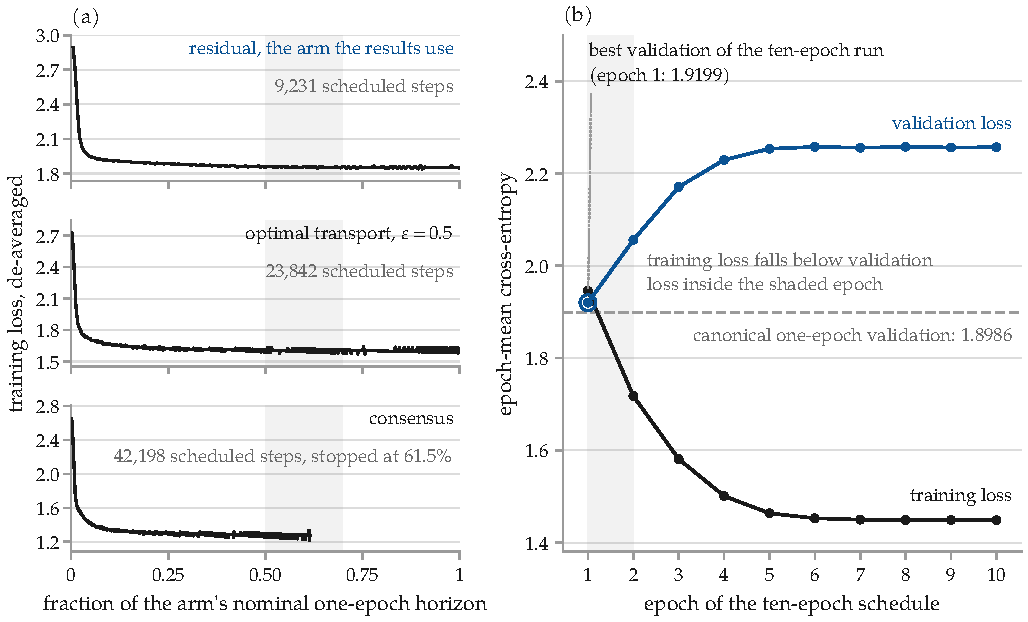
\includegraphics{fig-training}
\caption[The short-run arms flatten; a longer schedule
overfits]{\textbf{The canonical short-run arms flatten, while a
separate longer residual schedule overfits on held-out cross-entropy.}
(a) De-averaged training loss against fraction of the nominal one-epoch horizon,
three target constructions, each on \emph{its own} $y$-axis: absolute losses are
not comparable between arms because their target strings differ, so no shared
scale is offered. The residual and optimal-transport arms complete their epoch;
consensus was scheduled for one but terminated by the wall-clock at $61.5\%$,
where its line stops. Three superseded residual builds are omitted, as is the
single-cell arm, whose training log was not retained. Every arm runs a cosine
schedule annealing to $\approx 0$; the shaded band marks $50$--$70\%$ of the
horizon, where the residual arm's learning rate is still $22$--$52\%$ of its
post-warmup peak of $10^{-5}$ and its de-averaged loss travels only from $1.859$
to $1.854$. (b) Epoch-mean losses for the ten-epoch residual schedule (nominal
horizon $92{,}318$; $92{,}310$ optimizer updates). The ringed point is that
run's best validation loss, at epoch 1. The dashed line is the canonical
one-epoch run's validation loss on the same $3{,}600$-example file, $1.8986$,
which the ten-epoch run does not reach at any epoch. Training loss is above
validation at epoch 1 and below it at epoch 2, so the crossing falls inside the
shaded epoch; where inside it is not logged, and no point is drawn for it. Two
things this figure does not establish: that all possible learning-rate schedules
are ruled out, and that $\NIR$ worsens with additional epochs --- no long-run
checkpoint was scored with $\NIR$.}
\label{fig:training}
\end{fullwidth}
\end{figure}

% ===========================================================================
\begin{table}[htbp]
\begin{threeparttable}
\caption[Training configuration]{\textbf{One base checkpoint, one
hyperparameter set, five arms differing only in target.} Learning rate
$10^{-5}$, batch size 1, gradient accumulation 16, maximum length 8192, bf16,
weight decay 0.01, warmup ratio 0.03 throughout. The consensus arm stopped early
on a flat loss, so it is the $\varepsilon$-ladder's weakest-evidenced endpoint,
and at the residual arm's generation budget against a neutral partner the
optimal-transport endpoint is not null either (\cref{sec:res-encoding}); outside
\cref{tab:epsilon} the ladder's negative rests on the single-cell endpoint
alone. These five arms (\texttt{single\_cell}, \texttt{consensus},
\texttt{ot\_T2}, \texttt{residual}, \texttt{residual\_holdout}) are also the
complete family over which the identity test of \cref{sec:res-mechanism} takes
its multiplicity correction, five arms by up to seven depths and $26$ measured
tests, the family behind the $q$-values quoted there. One qualification attaches
to the residual row. Its step count is the rebuilt target build's, on which the
canonical behavioural results are scored, while the identity test of that arm
ran on the earlier target build.}
\label{tab:trainconfig}
\footnotesize
\begin{tabularx}{\linewidth}{@{}%
  >{\raggedright\arraybackslash}X
  >{\raggedright\arraybackslash}X
  l
  >{\raggedright\arraybackslash}X@{}}
\toprule
\thead{Arm} & \thead{Target} & \thead{Training} & \thead{Note} \\
\midrule
single cell & the observed treated cell & 1 epoch & \\
consensus & group pseudobulk & \textbf{$\approx 60\%$ of an epoch}
  & tier-1 $\NIR$ unscoreable \\
optimal transport (T2) & barycentric, $\varepsilon{=}0.5$
  & 1 epoch, 23{,}842 steps & \\
residual & signed residual & 1 epoch, 9{,}231 steps
  & rebuilt build's step count \\
residual (holdout) & as above, 738 withheld & 1 epoch & \\
\bottomrule
\end{tabularx}
\end{threeparttable}
\end{table}

\begin{scopelimit}[carried into \cref{sec:res-mechanism}]
The residual arm's two measurements are not on the same weights. The step count
recorded above is the rebuilt target build's, which is the build the canonical
behavioural results are scored on, whereas the identity test of that arm ran on
the earlier target build. A behavioural result for that arm and an activation
probe of it therefore come from two different builds, and this qualification
travels with any statement that pairs them.
\end{scopelimit}

\paragraph{How panel (a) must be read} Two properties of the one-epoch logs behind
\cref{fig:training} decide it. The trainer records a
\emph{cumulative} epoch mean, not an instantaneous loss, and that flattens by
arithmetic whatever the model is doing, so every series is de-averaged to its
per-window value before plotting. And the cosine schedule anneals the learning
rate to $\approx 0$ by the end of the epoch, $2.96 \times 10^{-10}$ at the last
logged step against a post-warmup peak of $10^{-5}$, so the final third of each
curve is flat partly because the step size has gone to zero, and is not
independent evidence of anything.

What is load-bearing is the band between $50\%$ and $70\%$ of the epoch, where
the learning rate is still $22$--$52\%$ of peak, enough to move the weights, and
the residual arm's loss has already flattened, travelling only from $1.859$ to
$1.854$. Its final held-out loss, on a matched validation file of $3{,}600$
examples, is $1.8986$ against a training loss of $1.8854$.

\paragraph{Panel (b) tests ordinary longer optimisation directly} Both residual
logs agree on base model and tokenizer,
training and validation files and counts, seed, effective batch, and peak logged
learning rate; weight decay and AdamW betas are not logged and are not claimed
as verified matches (\texttt{training\_adequacy\_}\allowbreak\texttt{long.json}). The ten-epoch run
has a nominal horizon of $92{,}318$ but executes $92{,}310$ optimizer updates,
accumulation resetting at every epoch boundary so that each epoch contributes
$\lfloor147{,}710/16\rfloor=9{,}231$. It is a separate longer schedule, not a
continuation; changing \texttt{num\_epochs} stretches the cosine schedule across
all ten epochs.

The result runs the wrong way for the objection. Validation loss is best at
epoch 1 ($1.9199$), worsens to $2.0559$ and $2.1708$ at epochs 2 and 3, and ends
at $2.2568$, while training loss falls from $1.9456$ to $1.4485$. The canonical
one-epoch run remains better on the same validation file ($1.8986$).

\begin{scopelimit}[carried into \cref{sec:limitations}]
That result does not show that every possible schedule would fail, and no
long-run checkpoint was scored with $\NIR$, so it says nothing about whether
$\NIR$ itself worsens with additional epochs. Together with the one-epoch
traces, it excludes undertraining as a \emph{trivial} explanation, not as a
general one.
\end{scopelimit}

% ===========================================================================
% PLACEMENT ONLY -- MOVED, not edited. This float used to be declared here, at
% the very end of A.4, some 40 lines after the \cref that introduces it. Two
% measured consequences, both gone now that it is declared next to its first
% reference (see the block above \paragraph{Panel (b)}):
%   1. It could not be placed until the builder was already on p.118, two pages
%      past the \cref on p.116.
%   2. Placed at the top of p.118 it left just enough room under itself for the
%      two \Large lines of the A.5 heading and nothing else, stranding that
%      heading at the foot of the page. \needspace cannot repair this from the
%      heading's side: it tests \pagegoal-\pagetotal in the main vertical list,
%      before the deferred float has been contributed to the page, so it reads a
%      full page of room and passes. VERIFIED: \needspace{10\baselineskip} on
%      the A.5 heading produced a byte-identical PDF. The float is the cause and
%      the float is what has to move.
% Neither the figure, its caption, nor one number in either was touched.

% ===========================================================================
\framedecl{-}
\section{Three identity-test designs failed, and each failure is a constraint on the fourth}
\label{sec:app-identity}

\begin{question}
The substitution test the body reports is the fourth design, and the three
before it each produced a result this thesis once quoted as a finding. The
instrument here is the algebra of each failure, what the control arm was
actually doing.
\end{question}

\noindent
All three failures below are failures of the control arm, not of the readout.
\Cref{fig:slab} draws the geometry each of them misses, and its three insets are
the three designs in the order they are argued here.

% ===========================================================================
% slab.tex -- "represented but not consulted", drawn.
% \input by Sections/04b-representation.tex inside \beatsection sec:res-used.
% Compiles against thesis_v2/preamble.tex and nothing else: no \includegraphics,
% no external data, no TikZ library beyond the ones preamble.tex already loads
% (this file uses arrows.meta, calc and decorations.pathreplacing).
%
% EVERY NUMBER DRAWN, AND WHERE IT COMES FROM
% -------------------------------------------
% Source: RESULTS_cluster/workspace_probe.json, key layers.<L>.variance_share,
% over the seven layers the probe ran (2, 4, 6, 8, 9, 12, 16). Config there:
% n_drugs 12, n_per_drug 40, n_dims 10, chance 0.08333. Sibling ledger of the
% exact values drawn: thesis_v2/figs/slab.json.
%
%   quantity            per-layer values (2,4,6,8,9,12,16)              mean
%   context        .701714 .738805 .756182 .749826 .741689 .838166 .838560  0.76642
%   cell_line      .579634 .641342 .665019 .667029 .654599 .567865 .492515  0.60971
%   drug_pure      .035747 .030703 .030347 .029881 .030620 .029807 .033109  0.03146
%
% The two WEDGE AREAS are the only scaled marks in the top panel:
%   context wedge   0.766420 of the disc -> 275.9113 deg
%   V_pure wedge    0.031459 of the disc ->  11.3252 deg
%   unshaded rest   0.202121 of the disc ->  72.7635 deg   (1 - the other two;
%                   the two subspaces are orthogonal, so the shares add and the
%                   remainder is what is left. It carries NO printed number.)
% Sum check: 275.9113 + 11.3252 + 72.7635 = 360.0000.
%
% AGREEMENT WITH THE TEXT (checked, not assumed):
%   04b-representation.tex:341  "stays flat at ~0.03 against ~0.6 for cell line"
%                               -> drawn 0.031 and quoted 0.610.               OK
%   04b-representation.tex:350  "cell line measures 15-22x the purified slab"
%                               -> per-layer ratios 14.9 16.2 19.0 20.9 21.4
%                                  21.9 22.3, i.e. 15-22x to two figures.      OK
%   04b-representation.tex:376  "flat at ~0.03, roughly 5% of the cell line's
%                               ~0.6"                                          OK
%   07-Appendix.tex:446-448     "roughly 99.5% of the control's energy ...
%                               cell-line directions at ~0.6 variance share"   OK
%   07-Appendix.tex:456-457     control delivers 5.3x the perturbation         OK
%   07-Appendix.tex:466         normaliser inflation "+2.75 nats"              OK
%   04b-representation.tex:260  "twelve centred class means span at most eleven
%                               directions"; top TEN kept (pure_drug_dims 10)  OK
% The context subspace's own share, 0.766, appears in NO sentence of the thesis;
% it is a new reading of the same JSON field, and it is labelled as the context
% subspace so it cannot be mistaken for the cell-line 0.61 the text quotes.
%
% INSET 1's ANGLE is a drawn quantity, not a decoration: a direction drawn
% isotropically in 2048 dimensions puts 10/2048 = 0.49% of its energy in a
% ten-dimensional slab, which is the appendix's "roughly 99.5%". An arrow at
% 86 deg to the slab axis has cos^2(86) = 0.0049 of its energy along that axis,
% so the arrow IS the number. Nothing else in the insets is to scale.
%
% LAYOUT NOTES, all forced by a build:
%   * fullwidth = textwidth 142mm + marginparwidth 28mm + marginparsep 4mm
%     = 174mm. Content is kept inside x in [0.00, 17.28]; a text-width block
%     starting at 12.00 must not exceed 5.20cm, because at 5.30cm the node's
%     inner sep pushed the picture 0.75pt over the measure and TeX said so.
%     (The "171mm" in preamble.tex's comment at \newenvironment{fullwidth} is
%     stale arithmetic; the geometry keys give 174mm.)
%   * the slab wedge is 11.3 deg wide and at radius 3cm is 5.9mm across at the
%     rim. Three class means and two arrows do not fit in it at true scale, so
%     the slab's interior is drawn ONCE, magnified, in the dashed panel, with
%     the two leader lines that make it a magnifier. The magnification is the
%     whole reason the size asymmetry can stay true: nothing was enlarged to
%     make a label fit.
%   * insets 2 and 3 repeat the leader-line device into their own small strips,
%     inset 1 does not. That is meaningful and not an inconsistency: failure
%     one happens OUTSIDE the slab and is legible at disc scale, failures two
%     and three happen inside it.
%   * the arm names sit UNDER mu_B and mu_C, not along the arrows. Along the
%     arrows they collided with each other in the wedge between them, because
%     the two displacements share an anchor; and mu_A had to be pushed left of
%     its dot, because directly above it is where Pi(mu_B - mu_A) begins.
% ===========================================================================
\begin{figure}[htbp]
\begin{fullwidth}
\centering
% --- the three wedge angles, computed above, written once --------------------
\newcommand{\slabHalf}{5.6626}     % half of 11.3252 deg  = 0.031459 of the disc
\newcommand{\slabCtxA}{5.6626}     % context wedge starts where the slab ends
\newcommand{\slabCtxB}{281.5739}   % 5.6626 + 275.9113
% --- one disc, drawn at whatever radius is asked for -------------------------
\newcommand{\slabdisc}[1]{%
  \filldraw[fill=panelbg, draw=rulegrey, line width=0.35pt]
    (0,0) -- (\slabCtxA:#1)
    arc[start angle=\slabCtxA, end angle=\slabCtxB, radius=#1] -- cycle;
  \filldraw[fill=accent, draw=accent, line width=0.3pt]
    (0,0) -- (-\slabHalf:#1)
    arc[start angle=-\slabHalf, end angle=\slabHalf, radius=#1] -- cycle;
  \draw[rulegrey, line width=0.5pt] (0,0) circle (#1);}

\begin{tikzpicture}[x=1cm, y=1cm, font=\footnotesize,
                    every node/.style={inner sep=1.6pt}]
  \tikzset{
    lab/.style     ={text=ink, font=\footnotesize},
    quiet/.style   ={text=quietink, font=\scriptsize},
    ttl/.style     ={text=accent, font=\scriptsize\bfseries\sffamily},
    lead/.style    ={draw=rulegrey, line width=0.3pt},
    swaparm/.style ={draw=accent, line width=1.0pt,
                     -{Latex[length=3.4pt,width=2.8pt]}},
    ctrlarm/.style ={draw=ink, line width=1.0pt,
                     -{Latex[length=3.4pt,width=2.8pt]}},
    dot/.style     ={circle, fill=ink, inner sep=0pt, minimum size=3.0pt},
    adot/.style    ={circle, fill=accent, inner sep=0pt, minimum size=3.4pt}}

% ###########################################################################
% # TOP BAND -- the stream, and the slab magnified
% ###########################################################################

  % ---------------- the disc ------------------------------------------------
  \begin{scope}[shift={(3.55,8.50)}]
    \slabdisc{3.0}

    \node[ttl, anchor=south] at (0,3.16)
      {THE 2048-DIMENSIONAL RESIDUAL STREAM};

    % the context subspace, labelled inside its own wedge
    \node[lab, align=center, text width=3.2cm] at (150:1.18)
      {\textbf{context subspace}\\ cell line, plate, dose};

    % the unshaded remainder carries no number
    \node[quiet, align=center, text width=2.1cm] at (318:1.95)
      {the remaining\\ directions};

    % the slab itself, too thin to hold a label
    \node[text=accent, font=\footnotesize, anchor=west]
      at (0:3.14) {$V_{\mathrm{pure}}$};

    % leaders to the magnified panel. Panel corners in OUTER coordinates are
    % (8.15,11.00) and (8.15,5.65); this scope's origin sits at (3.55,8.50).
    \draw[lead] (\slabHalf:3.0)  -- (4.60,2.50);
    \draw[lead] (-\slabHalf:3.0) -- (4.60,-2.85);
  \end{scope}

  % ---------------- the slab, magnified -------------------------------------
  \draw[rulegrey, line width=0.35pt, densely dashed, rounded corners=2pt]
    (8.15,5.65) rectangle (14.10,11.00);

  \node[ttl, anchor=north west] at (8.35,10.86) {THE SLAB, MAGNIFIED};
  \node[quiet, anchor=north west, align=left, text width=5.5cm] at (8.35,10.48)
    {at most ten of the $2048$ directions; $0.031$ of the stream's variance.
     The geometry below is schematic.};

  \coordinate (muA) at (9.40,7.90);
  \coordinate (muB) at ($(muA)+(30:2.05)$);
  \coordinate (muC) at ($(muA)+(-16:2.05)$);

  % equal norm, drawn as the one arc both heads land on
  \draw[rulegrey, line width=0.35pt, densely dashed]
    ($(muA)+(-16:2.05)$) arc[start angle=-16, end angle=30, radius=2.05];
  \node[quiet, anchor=west] at ($(muA)+(7:2.17)$) {identical norm};

  \draw[swaparm] (muA) -- (muB);
  \draw[ctrlarm] (muA) -- (muC);
  \node[lab, rotate=30,  anchor=south, inner sep=3pt]
    at ($(muA)!0.50!(muB)$) {$\Pi(\mu_B-\mu_A)$};
  \node[lab, rotate=-16, anchor=north, inner sep=3pt]
    at ($(muA)!0.50!(muC)$) {$\Pi(\mu_C-\mu_A)$};

  \node[adot] at (muA) {};
  \node[dot]  at (muB) {};
  \node[dot]  at (muC) {};
  \node[lab, anchor=east]       at ($(muA)+(-0.16,-0.06)$) {$\mu_A$};
  \node[lab, anchor=west]       at ($(muB)+(0.10,0.06)$)   {$\mu_B$};
  \node[lab, anchor=west]       at ($(muC)+(0.10,0.06)$)   {$\mu_C$};
  \node[quiet, anchor=west]     at ($(muB)+(0.10,-0.20)$)  {\textsc{swap} arm};
  \node[quiet, anchor=west]     at ($(muC)+(0.10,-0.18)$)  {\textsc{permuted} arm};

  \node[quiet, anchor=north west, align=left, text width=5.5cm] at (8.35,6.95)
    {Equal length is what makes \textsc{permuted} a matched control: same
     anchor, same construction, same norm, wrong drug.};

  % ---------------- the measured shares -------------------------------------
  \node[ttl, anchor=north west] at (14.30,10.86) {VARIANCE SHARE};
  \node[quiet, anchor=north west] at (14.30,10.50) {seven layers, mean};
  \draw[rulegrey, line width=0.4pt] (14.30,10.16) -- (17.25,10.16);
  \node[anchor=north west, text=ink, font=\scriptsize] at (14.30,10.06)
    {\begin{tabular}{@{}l@{\hspace{20pt}}r@{}}
       context & $0.766$\\[1.5pt]
       \textcolor{quietink}{cell line} & \textcolor{quietink}{$0.610$}\\[1.5pt]
       $V_{\mathrm{pure}}$ & \textcolor{accent}{$0.031$}\\
     \end{tabular}};
  \draw[rulegrey, line width=0.4pt] (14.30,8.86) -- (17.25,8.86);
  \node[quiet, anchor=north west, align=left, text width=2.90cm] at (14.30,8.74)
    {Only the wedge areas are drawn to scale. $V_{\mathrm{pure}}$ is
     orthogonal to the context subspace, so the two wedges share no direction.
     Cell line, the positive control, lies inside it, at $15$--$22\times$ the
     slab's share.};

% ###########################################################################
% # the divider
% ###########################################################################
  \draw[rulegrey, line width=0.4pt] (0,5.05) -- (17.25,5.05);
  \node[anchor=north west, font=\scriptsize\itshape, text=quietink]
    at (0,4.99) {three intervention designs failed on this geometry, and each
                 failure is a constraint on the fourth};

% ###########################################################################
% # INSET 1 -- mismatched geometry
% ###########################################################################
  \node[ttl, anchor=north west] at (0,4.60) {ONE\quad MISMATCHED GEOMETRY};

  \begin{scope}[shift={(1.25,2.92)}]
    \slabdisc{1.05}
    % 86 deg to the slab axis: cos^2(86) = 0.0049, i.e. 0.5% of the energy in
    % the slab and 99.5% outside it. The angle IS the number.
    \draw[ctrlarm] (0,0) -- (86:1.32);
    \draw[rulegrey, line width=0.3pt, densely dotted] (86:1.32) -- (0.092,0);
    \draw[accent, line width=1.8pt] (0,0) -- (0.092,0);
    \draw[lead] (0.12,0.02) -- (1.15,0.38);
    \node[quiet, anchor=west] at (0.16,1.15) {control};
  \end{scope}

  \node[quiet, anchor=west, align=left, text width=2.45cm] at (2.45,3.30)
    {its part inside the slab: $0.5\%$ of its energy};

  \node[lab, anchor=north west, align=left, text width=5.20cm] at (0,1.92)
    {The control was drawn in the full $2048$-dimensional stream while the
     intervention acts in at most ten directions, so $\approx 99.5\%$ of its
     energy lay where the hook never reached. ``The swap moves the prediction
     less than noise'' is what that geometry predicts, whatever the readout
     does.};

% ###########################################################################
% # INSET 2 -- ablate-then-add
% ###########################################################################
  \node[ttl, anchor=north west] at (6.00,4.60) {TWO\quad ABLATE-THEN-ADD};

  \begin{scope}[shift={(7.25,2.92)}]
    \slabdisc{1.05}
    \draw[lead] (\slabHalf:1.05)  -- (1.55,1.02);
    \draw[lead] (-\slabHalf:1.05) -- (1.55,-0.68);
  \end{scope}

  \begin{scope}[shift={(8.85,2.85)}]
    % added: an uncentred class mean = the shared global mean + its own part
    \node[quiet, anchor=south west] at (0,1.02) {added: $\mu_B$, uncentred};
    \fill[rulegrey!45] (0,0.84)    rectangle (1.25,1.00);
    \fill[accent]      (1.25,0.84) rectangle (2.00,1.00);
    % removed: the cell's own slab component, carrying the same global mean
    \node[quiet, anchor=south west] at (0,0.48) {removed: $\Pi h$};
    \fill[rulegrey!45] (0,0.30)    rectangle (1.25,0.46);
    \fill[accent]      (1.25,0.30) rectangle (1.70,0.46);
    \draw[rulegrey, line width=0.4pt, decorate,
          decoration={brace, amplitude=3pt, mirror}] (0,0.24) -- (1.25,0.24);
    \node[quiet, anchor=north] at (0.62,0.08) {$\bar m$, shared};
    % what the hook actually delivers
    \node[quiet, anchor=south west] at (0,-0.62) {what the hook delivers};
    \fill[accent] (0,-0.80) rectangle (0.30,-0.64);
    \node[quiet, anchor=west] at (0.40,-0.72) {$\bar m$ cancels};
  \end{scope}

  \node[lab, anchor=north west, align=left, text width=5.20cm] at (6.00,1.92)
    {The hook ablates before it adds, so what is delivered is
     (added $-$ removed), and an uncentred class mean shares its global-mean
     component with the thing removed. Substitution becomes restoration, and
     the control arm --- a real displacement --- delivers $5.3\times$ the
     perturbation.};

% ###########################################################################
% # INSET 3 -- the normaliser
% ###########################################################################
  \node[ttl, anchor=north west] at (12.00,4.60) {THREE\quad THE NORMALISER};

  \begin{scope}[shift={(13.25,2.92)}]
    \slabdisc{1.05}
    \draw[ctrlarm] (0,0) -- (2.2:0.95);
    \draw[lead] (\slabHalf:1.05)  -- (1.20,0.84);
    \draw[lead] (-\slabHalf:1.05) -- (1.20,0.06);
  \end{scope}

  % The four targets are drawn identically on purpose: the normaliser does not
  % know which of them carries identity, and that is the whole failure.
  \begin{scope}[shift={(14.45,2.92)}]
    \node[quiet, anchor=south west] at (0,0.84) {clean $\log P$};
    \draw[rulegrey, line width=0.4pt] (0,0.78) -- (1.70,0.78);
    \draw[rulegrey, line width=0.4pt] (0,0.06) -- (1.70,0.06);
    \foreach \x in {0.20,0.65,1.10,1.55}{
      \fill[ink] (\x,0.78) circle (1.5pt);
      \fill[ink] (\x,0.06) circle (1.5pt);
      \draw[quietink, line width=0.5pt, -{Latex[length=2.6pt,width=2.2pt]}]
        (\x,0.72) -- (\x,0.14);}
    \node[quiet, anchor=north west] at (0,-0.06) {the control arm};
    % anchor=west under rotate=90 puts the START of the string at this point and
    % grows it UPWARD, so the label spans the two rules it measures between
    % instead of hanging below the lower one. Centred at 0.42 it reached y=-0.23
    % and collided with the descender line of "the control arm".
    \node[quiet, rotate=90, anchor=west] at (2.04,0.10) {$+2.75$ nats};
  \end{scope}

  \node[lab, anchor=north west, align=left, text width=5.20cm] at (12.00,1.92)
    {A random direction \emph{inside} the slab inflates the logsumexp
     normaliser by a measured $+2.75$ nats, where the observed class-mean
     displacement does not. Every target is depressed by it, carrying identity
     or not: norm-matched is not disruption-matched.};

  % bounding box, so the picture is exactly the fullwidth measure
  \path (0,0.05) rectangle (17.28,11.75);
\end{tikzpicture}

\caption[The drug slab and the context subspace, by variance
share]{\textbf{The purified drug slab is a thin wedge of the residual stream
beside the context subspace, and each of the three failed identity tests turns
on that geometry.} The disc is the
$2048$-dimensional residual stream at one layer. \emph{The two wedge areas are
the only scaled marks in the figure}, drawn to the measured subspace variance
shares in \texttt{workspace\_probe.json} (twelve drug classes, forty cells
each, chance $0.083$), averaged over the seven probed layers: $0.766$ for the
context subspace of cell line, plate and dose, and $0.031$ for the purified
drug slab $V_{\mathrm{pure}}$. Cell line alone, the positive control, reads
$0.610$ and lies inside the context subspace, so it is quoted as a number
rather than drawn as a third wedge. $V_{\mathrm{pure}}$ is what remains after
the drug slab --- spanned by at most eleven directions, since it is built from
twelve centred class means, of which the top ten are kept --- is orthogonalised
against that context subspace, which is why the two wedges share no direction.
The unshaded remainder closes the disc and carries no number. Everything else
is schematic and has no scale: the slab is $11.3^{\circ}$ wide and cannot hold
three class means at true size, so its interior is magnified, where the
\textsc{swap} and \textsc{permuted} displacements are drawn at equal length
because equal length is what makes \textsc{permuted} a matched control. The one
exception among the insets is inset one's angle, which is drawn true: a
direction drawn isotropically in $2048$ dimensions puts $10/2048$ of its energy
in a ten-dimensional slab, the appendix's $\approx 99.5\%$ lying outside it. No
decode accuracy, layer axis or KL divergence appears here; those are
\cref{fig:mechanism}. The three insets are the failed designs of
\cref{sec:app-identity}.}
\label{fig:slab}
\end{fullwidth}
\end{figure}



\paragraph{Failed design one, mismatched geometry} The first test overwrote drug
A's code with drug B's inside a $\leq 10$-dimensional purified subspace, and
compared the resulting KL against a random vector of identical norm drawn in the
\emph{full} $2048$-dimensional stream. Roughly $99.5\%$ of the control's energy
then lay where the intervention never reached, including the cell-line
directions at $\approx 0.6$ variance share. ``The swap moves the prediction less
than noise'' is what that geometry predicts, whatever the readout does.

\paragraph{Failed design two, ablate-then-add} The second drew the control
inside the subspace, which looked like a repair. The hook ablates
before adding, so what is delivered is (added $-$ removed), and an uncentred
class mean shares its global-mean component with the thing removed. The
substitution arm was then close to a restoration, the control arm a real
displacement. Simulated with no model present, the control delivers $5.3\times$
the perturbation in $100\%$ of draws, predicted gap
$2\langle \mu_B, u\rangle = 9.179$ against an observed $9.162$, with $\mu_B$ the
injected class mean and $u$ the cell's component in the slab. The retracted
result was geometry, not biology.\corrmark{The ablate-then-add identity result,
retracted as an artefact of the hook's own algebra.}

\paragraph{Failed design three, the normaliser} The third injected the
displacement and scored $\Delta \log P(g_B)$ against a norm-matched random
direction, and was confounded the opposite way. A random direction inside the
slab inflates the logsumexp normaliser (measured $+2.75$ nats) where the
observed class-mean displacement does not, so every target is depressed under
the control arm whether or not it carries identity. With the scored target
stripped of all identity information, $36\%$ of the effect still stood.
Norm-matched is not disruption-matched.

That argument also retires the simplest \emph{injection} test, ``how far did the
prediction move''. Distance moved is what norm-matching equalises, so the test
has no power in precisely the world where the readout does read the drug. It
does not reach the behavioural output-invariance instrument of
\cref{sec:methods-controls}, which perturbs the prompt and matches no norms;
that instrument's own limitation, registering whether the generated text moves
and not whether it moves correctly, is stated where it is used.

\paragraph{Three further guards are engineering, not inference} A
\emph{drug-proxy screen} refuses any context label that is a near-bijection with
drug; it caught \texttt{dose\_float} holding a sample identifier in the residual
builders, a label that would have deleted the drug axis had the builders
orthogonalised against it. An \emph{injected-norm diagnostic} reports the
displacement against the cell's centred slab component ($0.69$--$1.40$), so the
injection is the size of the thing it displaces and a null cannot be blamed on a
whisper. A \emph{selftest with teeth} runs three planted worlds
(drug inert, drug read, and drug inert behind a readout sensitive to magnitude
and not direction) through the headline code path, separates them ($-0.042$,
$+1.520$, $-0.010$), and failed four times in development, each failure a real
defect the guard list now covers.

\begin{scopelimit}[carried into \cref{sec:res-mechanism}]
The third planted world is not a normaliser control. Each planted response is a
single token, so nothing diverges, and the state-dependent part of the
normaliser is precisely what the selftest cannot exercise. What separating the
three worlds licenses is the code path the selftest runs them through.
\end{scopelimit}

% ===========================================================================
\framedecl{ER}
\section{The metric exploit is a property of the metric, not of one baseline}
\label{sec:app-selftest}

\begin{question}
A metric audit whose own instrument is untested proves nothing, and the exploit
it turns on was demonstrated with a single construction. The instrument here is
a second, independent zero-information baseline put through the same framework.
It saturates the standard metric too.
\end{question}

\noindent
The self-test does the deterministic things first (a perfect prediction reaches
the metric's maximum, a zero shift and a flat truth return no score), then the
thing that matters. It asserts the exploit under a \emph{second, independent}
zero-information baseline, where a leave-one-out mean scores $\DEdr = 1.000$
while $\NIR$ refuses to place it above chance. The coded assertion is
$\NIR \leq 0.6$; the recorded value is $0.000$.

\paragraph{What that $0.000$ is not} It is not the metric's chance value,
$0.500$ (\cref{sec:methods-metrics}), which is what the generic arm scores in
\cref{tab:lookup} and \cref{tab:allarms}. Nor is it the untied degeneracy that
section describes, since the self-test uses the same half-tie convention as
everything else. It is a property of this construction. The mean of the five
other drugs resembles those five more closely than the held-out one, so it loses
every comparison.

Two unrelated constructions saturate the standard metric, and the discrimination
metric places neither above chance. One would leave the standard metric merely
unlucky; two make the exploit a property of the metric.


% The reference apparatus: symbol table, term glossary, the two measurement
% frames, the three hedge registers, and the record of corrections. MOVED HERE
% FROM THE FRONT. It opened the document until the first full draft, where it
% put ~14 pages of lookup tables between the reader and the first sentence of
% the argument -- the reader met the vocabulary before meeting anything that
% needed it. It is reference, consulted on demand and not read through, so it
% belongs at the back with the other reference matter. The Introduction carries
% a forward pointer to it; nothing in the argument requires reading it first.
% ===========================================================================
% 00-HowToRead.tex -- the reference apparatus. UNNUMBERED, sits after the
% Appendix. MOVED FROM THE FRONT: it is looked up, not read through.
% Contents: the two measurement frames, the three hedge registers, the page
% furniture, the symbol table, the term glossary, the record of corrections.
%
% This is where the vocabulary is fixed, so it is the file that has to be
% right: one referent, one word. drug (never compound, molecule or agent);
% cell line; condition; treated well; shift / generic / residual; prediction;
% prompt; cell sentence. Words the drafts retired keep an entry of their own,
% so a reader who meets one in an older file can find where it went.
%
% NO claim block and NO \claimlede: this chapter reaches no verdict, and it
% introduces, strengthens and weakens nothing. It only fixes the vocabulary.
% Box budget used here: one scopelimit. Cap is three.
% ===========================================================================

\chapter*{Reference apparatus}
% \phantomsection must precede \addcontentsline so the hyperref anchor lands on
% this page, and \label must follow it so nameref picks up "Reference
% apparatus" from \@currentlabelname. 01-Introduction.tex refers here with
% \nameref, not \cref: this is \chapter*, so it owns no counter and cleveref
% would print whatever number was last stepped (a section of Appendix A).
\phantomsection
\addcontentsline{toc}{chapter}{Reference apparatus}
\label{sec:howtoread}
\markboth{REFERENCE APPARATUS}{}
\framedecl{-}

\begin{question}
Every term, symbol and convention that carries weight across more than one
chapter is fixed here, with the record of the six withdrawn claims.
\end{question}

\noindent
Where an interval exists, a number is quoted as a value followed by its
bracketed lower and upper bounds, a two-way cluster-robust $95\%$ interval
unless stated otherwise.\seealso{\cref{fig:timeline} maps the nine beats in
order}

% ---------------------------------------------------------------------------
\section*{Two measurement frames, one chance value}

\noindent
The two frames score different objects against different competitors, and they
both put chance in the same place. Comparing a number from one with a number
from the other is the most expensive misreading available in this
thesis.\framecue{\Eframe\ \Rframe}{in every running head}

In the \Eframe{} \emph{expression frame} the prediction is a cell profile,
scored against other drugs on the same plate. In the \Rframe{} \emph{residual
frame} it is the drug-specific residual, what survives once the generic
programme has been subtracted, scored against other drugs in the same cell
line. In both frames the \emph{comparison set} $J$, the conditions a prediction
is ranked against, fixes chance at $0.50$, and $J$ is declared explicitly at
every score.

\paragraph{Where the trap is} Because chance is $0.50$ in both frames, two
numbers that look alike invite subtraction. They may not be subtracted.
The residual frame's within-well precision reference is $0.854$
where the expression frame's is $0.576$, so the $0.537$ in one frame and the
$0.498$ in the other are not two attempts at one task
(\cref{sec:res-summary}).\seealso{\cref{fig:frames} draws the residual
construction}

\paragraph{How to tell which is in force} Three redundant cues say so. Every
section declares its frame in its opener as a chip, \Eframe{} or
\Rframe{}, shape and word before colour so that the cue survives greyscale; the
running head repeats it on every page; and a margin cue marks any change of
frame inside a section. A head naming no frame asserts nothing in either, as
here and in the apparatus of \cref{sec:methods-data}.

% PLACEMENT ONLY. Six lines and a framed header, splitting four and two across
% the page turn, so the two-line remainder opened the next page with neither the
% header nor a rule above it and read as loose prose. 9 lines is the box entire.
\needspace{9\baselineskip}%
\begin{scopelimit}[carried into every chapter]
A distance to a reference is comparable within a frame and not between frames.
The same restriction holds \emph{within} a frame across
supports: populations selected by different rules are not one population. Where
this thesis quotes two numbers side by side it names the population each was
computed on; where no population is named, they are not being compared.
\end{scopelimit}

% ---------------------------------------------------------------------------
\section*{Three registers of qualification}

\noindent
There are exactly three registers and no fourth.\gloss{register}{The three
kinds: a limit carried forward, a correction on record, and ordinary inline
care.}

\begin{description}[leftmargin=1em, itemsep=0.5ex,
                    font=\normalfont\bfseries]
\glentry{A scope limit}{scopelimit} fences in what a number \emph{licenses}, and
  the reader has to carry it forward. The test: would a later section be
  entitled to say something different if this sentence did not exist? Its tag
  names where the limit carries to.
\glentry{A correction}{correction} marks a withdrawal this thesis makes against
  itself. Six are withdrawn \emph{claims}, indexed in \cref{tab:corrections}, so
  that set is bounded and countable; the rest retract a defective piece of
  apparatus --- a voided control, a mis-resampled interval, a replaced
  instrument, a leaking partner pool. Each mark of either kind stands where the
  withdrawal is argued.
\glentry{Routine qualification}{routine} stays inline and unmarked, in the
  sentence it qualifies, and most of the qualification in this thesis is of this
  kind. It is not a lesser statement for being unmarked, only one the reader
  need not carry anywhere.
\end{description}

\paragraph{Two phrases that are not synonyms} \notestablished and \shownzero
are different statements.
A measurement that fails to separate two arms has established nothing about
their difference. It has not shown the difference to be zero. Where an interval
spans zero, this thesis says which of the two it means.

\paragraph{And two more that are not} Excluding zero is not the same as clearing a
pre-spec\-i\-fied relevance margin, and spanning zero is not evidence of
equivalence. Two margins are pre-registered, on different quantities and
different instruments.

\begin{description}[leftmargin=1em, itemsep=0.5ex,
                    font=\normalfont\bfseries]
\glentry{relevance margin}{relmargin} The pre-set $0.03$, in $\NIR$ units, that
  a channel's interval has to clear on the gate of \cref{sec:res-scope} before
  the channel is called live.
\glentry{materiality margin}{matmargin} The pre-registered $10\%$ of the model's
  own clean preference gap, on the identity test of \cref{sec:res-mechanism}. An
  effect inside it is too small to be called material.
\end{description}

Where a pre-registered margin exists the verdict vocabulary is fixed in advance,
three states plus a fourth for a control that could not be built.

\begin{description}[leftmargin=1em, itemsep=0.5ex,
                    font=\normalfont\bfseries]
\glentry{live}{live} The interval clears the pre-set $0.03$ relevance margin on
  the clustering axis appropriate to the claim. The axis is written into the
  verdict, because the word is not usable without it.
\glentry{closed}{closed} The interval lies wholly below that margin.
\glentry{inconclusive}{inconclusive} Neither. This includes an interval that
  excludes zero but straddles the margin, and it is not equivalence with the
  null.
\glentry{untestable}{untestable} The plate-matched null spans too few cell lines
  to be built here. ``We could not build the control'' must never be written as
  ``closed''.
\end{description}

% ---------------------------------------------------------------------------
\section*{Reading the page}

\noindent
A number a sentence \emph{asserts} goes in the body, always, with its interval,
its comparison set and its reference beside it. A number it merely
\emph{recalls} may go in the margin column, bare, with a pointer to where it was
established.\gloss{margin column}{Definitions, landmark constants, frame cues
and pointers; never an assertion.} Delete every margin note and the body must
still be complete and correctly qualified.

\paragraph{Five shapes} A section \emph{opener} states the question and the
instrument built to answer it, in words, with no numbers; the beat strip that
goes with it is the investigation's nine beats with the current one filled, and
no cell filled means the section is not one of the nine, as here. A \emph{claim
block}, hairlined above and below, carries the verdict in language that could be
shown wrong. \Cref{sec:res-field} closes without one, deliberately: it asks which span
of the prompt the model reads, cannot answer, and ends in the open question. A
\emph{definition} sits in a tinted panel with no rules. A \emph{scope limit} and
a \emph{correction} are the two marked hedge registers above.

\paragraph{The audit flag} A tinted value carrying a raised query mark is a
quantity this draft does not settle and a rerun will; three are open. The prose
around such a value holds whichever way it moves, and where that could not be
done the argument was not made. No such flag should survive into a submitted
copy.

% ---------------------------------------------------------------------------
\section*{Symbols}

\noindent
Fixed for the whole document, never redefined in a section.

\begin{description}[labelwidth=5em, leftmargin=6em, labelsep=0.6em,
                    style=multiline, font=\normalfont, itemsep=0.5ex]
\glentry{$\NIR$}{nir} \emph{Normalised inverse rank.} The fraction of a declared
  comparison set whose truth a prediction resembles less than it resembles its
  own, with ties counted at one half. Chance is $0.50$ under the exchangeability
  condition audited in \cref{sec:res-metrics}.
\glentry{$\DRF$}{drf} \emph{Dynamic range fraction.} Not a performance score but
  a meta-metric. It fixes a scale with an uninformative predictor at zero and a
  perfect predictor at one, then asks how far up that scale a candidate metric
  places a positive control of known quality (the interpolated duplicate in the
  expression frame, a raw split-half in the residual frame,
  \cref{sec:methods-data}).
\glentry{$\DEdr$}{dedr} The field's standard differential-expres\-sion
  delta-cor\-re\-la\-tion, the correlation between predicted and true change
  from control, restricted to the genes with the largest true change.
\glentry{$\paneltau$}{paneltau} Kendall's $\tau$ between predicted and true rank
  over the full $946$-gene panel. It selects no gene subset.
\glentry{$\gap$}{gap} The scramble gap, $\NIR$ of the model minus $\NIR$ of the
  scramble.
\glentry{$\Tcoef$}{tcoef} The disattenuated transfer coefficient, measuring how
  much of a drug's response is shared across cellular contexts. It is a
  similarity coefficient, not a variance share.
\glentry{$\resid$}{resid} The drug-specific residual, $\resid(d,c)$: what is
  left of the shift once the generic programme has been subtracted from it. The
  scored object in \Rframe.
\glentry{$\shift$}{shift} The treated-minus-control shift, $\shift(d,c)$: the
  treated pseudobulk minus its plate-matched control pseudobulk, and nothing
  else. An arithmetic object, not a verdict about the drug.
\glentry{\ENDCELL}{endcell} The registered atomic token that terminates a cell
  sentence.
\glentry{\DOWN}{down} The registered atomic token marking the up\slash down
  boundary in a residual target. Left unregistered it splits into sub-words and
  the boundary ceases to be a clean symbol.
\glentry{\Eframe}{eframe} Page furniture, not a quantity. The expression frame
  is in force here.
\glentry{\Rframe}{rframe} Page furniture, not a quantity. The residual frame is
  in force here.
\end{description}

% ---------------------------------------------------------------------------
\section*{Terms}

\noindent
Defined once, used in that sense everywhere.\seealso{\cref{sec:methods-data}
builds the apparatus these terms name}

\paragraph{One referent, one word} A synonym reads as a second object. These
are the words the drafts converged on, with the ones they gave up.

\begin{description}[leftmargin=1em, itemsep=0.5ex,
                    font=\normalfont\bfseries]
\glentry{drug}{drug} The perturbagen, whatever its chemistry.
  \emph{Compound}, \emph{molecule} and \emph{agent} are not used as synonyms for
  it; \emph{small molecule} appears only where the class of thing the atlas
  contains is what is meant.
\glentry{cell line}{cellline} The biological context. Two words as a noun,
  hyphenated only as a compound adjective, as in \emph{cell-line-specific}. The
  bare \emph{line} stands in where the paragraph has already fixed the referent.
\glentry{shift, generic, residual}{quantities} Three objects, never
  interchangeable: the \emph{shift} is treated minus control, the
  \emph{generic} is the drug-agnostic mean response subtracted from it, and the
  \emph{residual} is what remains. \emph{Response} keeps its ordinary
  biological sense and \emph{effect} its ordinary one; neither stands in for
  the residual.
\glentry{prediction}{prediction} What the model produces and what gets scored.
  \emph{Generation} names the act of decoding and only that. \emph{Output} is
  not used as a noun for it, and survives only inside the
  fixed instrument name \emph{output invariance}, which names a test and not
  the thing predicted.
\glentry{readout}{readout} Two senses, and the surrounding sentence fixes which.
  Biologically, what the sequencing reports. Of the model, the decoding stage
  that turns the residual stream into a sentence, the second term of the
  \emph{representation and readout} distinction \cref{sec:limitations} turns on,
  for which \emph{decoder} is the alternative word. Neither sense names the
  prediction, which is what that stage emits.
\glentry{prompt}{prompt} What the model is given at inference: a cell sentence,
  the drug name, the dose and the mechanism field.
\glentry{profile}{profile} A ranked expression vector. Not a synonym for
  \emph{sentence}, which is the encoding of one cell.
\glentry{sample (retired)}{sample} Earlier drafts used the word for the scored
  unit and for the physical one, which made two objects look like one. Neither
  now: the scored unit is a \emph{condition}, the physical one a \emph{treated
  well}. \emph{Observation} is not used for either.
\glentry{signature (retired)}{signature} Bare \emph{signature} names nothing
  here. \emph{Drug-specific signature} is allowed once, to gloss
  \emph{residual} on first use; after that the word is \emph{residual}.
\end{description}

\paragraph{Units of analysis}

\begin{description}[leftmargin=1em, itemsep=0.5ex,
                    font=\normalfont\bfseries]
\glentry{condition}{condition} A (drug, cell line, plate, dose) tuple. It is the
  unit that gets scored.
\glentry{treated well}{treatsample} The physical treatment assignment. Conditions
  nest inside it, so a well is not itself a condition and the two are not
  counted against each other.
\glentry{batch unit}{batchunit} The pair (cell line, plate), never the plate
  label alone, because plates are numbered within cell line and not globally.
\glentry{pseudobulk}{pseudobulk} The mean expression profile of a group of
  cells. A \emph{control pseudobulk} is the same object over plate-matched DMSO
  cells.
\glentry{dose}{dose} A molar concentration resolved from
  \texttt{drugname\_drugconc}, carried as a concentration and never as a
  unitless float.
\glentry{cell sentence}{cellsentence} A cell written as its expressed panel
  genes in descending order of expression, terminated by \ENDCELL. The encoding
  discards expression magnitudes and retains ranks.
\end{description}

\paragraph{Frames and comparison sets}

\begin{description}[leftmargin=1em, itemsep=0.5ex,
                    font=\normalfont\bfseries]
\glentry{expression frame}{exprframe} Scores a predicted cell profile against
  other drugs on the same plate; conditions grouped by (cell line, plate).
\glentry{residual frame}{residframe} Scores a predicted residual against other
  drugs in the same cell line, after the generic programme is subtracted;
  conditions grouped by cell line.
\glentry{comparison set $J$}{compset} The conditions a prediction is ranked
  against. It fixes chance at $0.50$ in both frames and is declared wherever a
  score is quoted.
\glentry{within-well split-half precision reference}{reference} The score
  obtained when a disjoint cell subset of the same treated well is substituted
  for the prediction, recomputed for every stratum scored. One estimator, not
  several; what varies between settings is the frame, the comparison set and the
  cell budget. It is a sampling-precision estimate, optimistic relative to true
  biological reproducibility: not a biological replicate, and not the maximum
  predictable fraction of biology.
\glentry{ceiling}{ceiling} A shorthand for the reference above, used wherever a
  result is stated as a distance from it. The one exception in this document is
  the $\DRF$ positive control of \cref{sec:res-metrics}, which is not a row of
  \cref{tab:ceilings}.
\glentry{noise ceiling (retired)}{noiseceiling} Earlier drafts joined
  \emph{ceiling} to a word for error, which invited reading the value as a
  bound on achievable performance. It is a two-cell precision estimate. Where
  \cref{sec:res-metrics} needs the quantity it names the construction, the
  $\DRF$ positive control or a row of \cref{tab:ceilings}.
\glentry{identifiability}{identifiability} A property of a single condition, not
  of a drug, and distinct from the aggregate references above. The
  condition's own within-plate split-half $\NIR$ against its plate-mates clears
  $0.8$.
\end{description}

\paragraph{Target construction}

\begin{description}[leftmargin=1em, itemsep=0.5ex,
                    font=\normalfont\bfseries]
\glentry{generic}{generic} The drug-agnostic mean response subtracted to form
  the residual, operationally the mean shift over the other drugs at the stated
  scope. It is conventionally read as the stress and cell-cycle programme common
  to all drugs, a reading used for intuition and nowhere tested.
\glentry{residual target}{residtarget} What remains once the generic is removed.
  Built \emph{split-before-fit} and \emph{leave-one-drug-out}.
\glentry{split-before-fit}{splitfirst} The holdout is fixed from metadata before
  any statistic is estimated, so no held-out target is defined partly by other
  held-out conditions.
\glentry{leave-one-drug-out}{lodo} No condition's generic contains its own drug,
  so the two sides of the split are scored against identically defined targets.
\glentry{scope}{scope} The set of drugs the generic mean is taken over, either
  \texttt{cell\_line} or \texttt{plate}. The choice is consequential.
\glentry{quota}{quota} The explicit per-split sampling rule, used because a
  uniform draw reproduces the pool's proportions and starves the held-out
  splits.
\glentry{training arm}{arm} A model variant differing from the others only in
  its training target or objective; five are used, cold-started from the same
  base checkpoint with identical hyperparameters, so that it is the only
  variable. The bare word \emph{arm} also names any one
  side of a paired comparison (a split, a run, a channel, a baseline), and is
  qualified wherever the surrounding sentence does not fix the sense. An
  unqualified \emph{arm} is not necessarily one of the five.
\end{description}

\paragraph{Baselines, splits and references}

\begin{description}[leftmargin=1em, itemsep=0.5ex,
                    font=\normalfont\bfseries]
\glentry{\texttt{control\_copy}}{controlcopy} The baseline that predicts the
  untreated cell unchanged. It carries zero drug information by construction,
  and it is the actual zero-shift predictor.
\glentry{\texttt{revert\_center}}{revertcenter} A predictor that places every
  gene at the middle rank. It carries no information about drug, cell or
  biology, and it is \emph{not} zero-shift.
\glentry{drug lookup}{druglookup} This drug's mean residual, estimated from
  training conditions in other cell lines. It needs no model, no prompt and no
  checkpoint.
\glentry{\texttt{moa\_lookup}}{moalookup} The same construction over drugs
  sharing this drug's mechanism annotation, on its own narrower support.
\glentry{channel}{channel} An annotated drug property --- protein target,
  mechanism, chemistry --- an unseen drug might be reached through. For a
  channel $X$, a drug's residual is predicted as the mean residual of the other
  drugs in the same cell line sharing property $X$ with it: \texttt{moa\_lookup}
  generalised from mechanism to any annotation. It is called live, closed,
  inconclusive or untestable against a plate-matched null differing in the
  channel alone (\cref{sec:res-scope}).
\glentry{scramble}{scramble} The prompt left byte-identical except that the
  drug name and mechanism are replaced by another drug's, while the control cell
  and the scoring truth are unchanged. It is the only manipulation that isolates
  drug use. Its \texttt{near}, \texttt{orth} and \texttt{opposite} strata are
  fixed by the measured cosine between the partner's residual and the target's,
  so a stratum's neutrality is an empirical property of these data and not a
  consequence of its construction.
\glentry{tiers}{tiers} The three evaluation tiers of the broad
  characterisation, defined by what the training set contained. \emph{Tier 1}:
  the (drug, cell line) pairing was seen, so it measures fit, not
  generalisation. \emph{Tier 2}: the drug never appeared (Leave-Drugs-Out).
  \emph{Tier 3}: drug and cell line were each seen but never together
  (Leave-Pairs-Out).
\glentry{\texttt{train} / \texttt{unseen\_combo} /
  \texttt{unseen\_drug}}{residsplit} The residual arm's own three-part split.
  \texttt{unseen\_}\allowbreak\texttt{combo} is an unseen \emph{well} of a seen
  drug, so it tests
  recombination and not full novelty.
\glentry{held out}{heldout} Held out from Tahoe fine-tuning, with the mechanism
  annotation still supplied in the prompt. Not absent from the model's prior
  world knowledge. Every unseen-drug result must be read under that narrower
  scope.
\end{description}

% ---------------------------------------------------------------------------
\section*{The record of corrections}

\noindent
Six claims that this thesis printed are withdrawn by this thesis.
\Cref{tab:corrections} indexes them, so the set is countable. Each is argued in
full in the section the table names. Corrections to the apparatus rather than to
a claim carry the same margin mark but are not tabulated here; each stands where
the repair is argued.

\begin{table}[!ht]
\begin{threeparttable}
\caption[The six corrections this thesis records against itself]{\textbf{The
six corrections this thesis records against itself.} Each row points at the
place the withdrawal is argued. Three of the six are argued in a numbered box;
the rest in the prose of the section named.}
\label{tab:corrections}
\footnotesize
\begin{tabularx}{\linewidth}{@{}%
  >{\raggedright\arraybackslash}p{0.30\linewidth}
  >{\raggedright\arraybackslash}X
  >{\raggedright\arraybackslash}p{0.11\linewidth}@{}}
\toprule
\thead{The claim withdrawn} & \thead{What killed it} & \thead{Where} \\
\midrule
The stronger mechanistic story earlier drafts told about the activation swap
  & Three substitution designs in turn: a control drawn in the full residual
    stream put almost all its energy where the intervention never acts;
    ablate-then-add turned the substitution arm into a restoration; and a
    norm-matched random direction inflated the normaliser. The retracted result
    was geometry, not biology.
  & \cref{sec:res-mechanism} \\
\addlinespace
The retention argument for a cell-line-scoped generic
  & Both retention figures were computed with a shared control pseudobulk
    subtracted from both halves, which correlates the halves through their
    common control error and favours cell-line scope precisely because the
    cell-line generic is itself less noisy.
  & \cref{sec:methods-residual} \\
\addlinespace
That the optimal-transport arm achieved nothing
  & The generation budget. Scored at the shorter token cap the arm's gap spanned
    zero and was printed as inert; re-run at the budget the residual arm had, it
    does not. The token budget is part of the claim.
  & \cref{sec:res-encoding} \\
\addlinespace
A training-exposure or memorisation advantage on trained conditions
  & Composition. Restricting the comparison to the drugs present in both arms
    reverses the sign, and the two arms are scored on populations selected by
    different rules.
  & \cref{sec:res-generalisation} \\
\addlinespace
That the model reads the drug name and not the mechanism field
  & The comparator. Those arms were scored against an \texttt{opposite}-stratum
    partner, which inflates every gap read against it, and because that is a
    property of the swap partner and not of the target build, it survives the
    re-run.
  & \cref{sec:res-field} \\
\addlinespace
That a swing in the held-out-drug control was evidence of seed instability
  & The comparator, and the draw. Both superseded figures are gaps against the
    \texttt{opposite} swap, which \cref{sec:res-generalisation} shows is not a
    null; and unseeded \texttt{do\_sample} advanced from global torch state, so
    the two arms of a contrast were drawn from different points of one stream.
    The diagnosis named the trigger and missed the cause.
  & \Cref{sec:limitations} \\
\bottomrule
\end{tabularx}
\begin{tablenotes}[flushleft]\footnotesize
\item Withdrawing a claim is not the same as establishing its negation. Each row
records that the evidence offered will not carry the claim, and leaves the
underlying question where the section arguing the withdrawal says it leaves it.
\end{tablenotes}
\end{threeparttable}
\end{table}

The same controls that produced these six shape the surviving design, among
them a zero-information baseline that improved when plate was free to vary; a
swap-distance sweep after a similar-drug scramble proved weak; a removal gate
before any ablation null; matched-norm injection before interpreting a swap;
intervals clustered on the units that repeat, cell line, drug and treated well,
never on cells; and a pre-registered three-state
interpretation whose inconclusive branch was allowed to fire. That record is why
the remaining claims can be read at the strength stated here, and no stronger.


\end{document}
